\documentclass[10pt,a4paper]{extreport}
\usepackage[top=1.0in, bottom=1.0in, left=1.0in, right=1.0in, heightrounded]{geometry}
\usepackage{ryan}
\usepackage[bottom]{footmisc}
\usepackage{pdfpages}

\pagestyle{fancy}
\fancyhf{}
\fancyhead[L]{\nouppercase{\leftmark}}%\slshape
\fancyhead[R]{\thepage}
\renewcommand{\headrulewidth}{0.4pt}
\renewcommand{\arraystretch}{1.5}

\usepackage[
backend=biber,
style=alphabetic,
sorting=anyt
]{biblatex}
\addbibresource{biblio.bib}

\makeglossaries

\newacronym{smo}{SMO}{Singapore Mathematics Olympiad}
\newacronym{h3math}{H3M}{H3 Mathematics}
\newacronym{h2fmath}{H2FM}{H2 Further Mathematics}
\newacronym{mat}{MAT}{Oxford Maths Admissions Test}
\newacronym{putnam}{Putnam}{William Lowell Putnam Mathematics Competition}
\newacronym{imo}{IMO}{International Mathematics Olympiad}
\newacronym{usamo}{USAMO}{United States of America Mathematical Olympiad}
\newacronym{apmo}{APMO}{Asian Pacific Mathematics Olympiad}
\newacronym{australia}{Australia}{Australian Mathematical Olympiad}
\newacronym{cmo}{China}{China Mathematical Olympiad}
\newacronym{canada}{Canada}{Canadian Mathematical Olympiad}
\newacronym{italy}{Italy}{Italian Mathematical Olympiad}
\newacronym{vietnam}{Vietnam}{Vietnam Mathematical Olympiad}
\newacronym{tstst}{USA TSTST}{United States of America Team Selection Test Selection Test}
\newacronym{arml}{ARML}{American Regions Mathematics League}
\newacronym{tripos}{Tripos}{Mathematical Tripos}

\begin{document}
\begin{titlepage}
\title{\sffamily\bfseries Mathematics Olympiad:\\[1ex] A Guidebook}
\author{Ryan Joo Rui An}
\date{}
\end{titlepage}

\maketitle
\pagebreak

\pagenumbering{roman}
\

\vfill

\begin{quote}
\textit{You don't have to be a mathematician to have a feel for numbers.}

\begin{flushright}--- John Forbes Nash, Jr. (1928--2015)\\
American mathematician
\end{flushright}
\end{quote}

\vfill

Copyright \copyright \ 2024 by Ryan Joo Rui An. 
Text licensed under \href{https://creativecommons.org/licenses/by-sa/4.0/}{CC-by-SA-4.0}. Source files licensed under \href{https://choosealicense.com/licenses/gpl-3.0/}{GNU GPL v3}.

This is (still!) an incomplete draft. Please send corrections and comments to \url{ryanjooruian18@gmail.com}, or pull-request at \url{https://github.com/Ryanjoo18/math-olympiad}.

Typeset using \LaTeX.

Last updated \today.
\thispagestyle{empty}
\pagebreak

\setcounter{page}{1}
\section*{About the Author}
\textbf{\sffamily Ryan Joo Rui An} is a dedicated and passionate high school student currently engaged in A Level studies in Singapore. With a strong foundation in mathematics, He has spent over 11 years honing his skills in various mathematics competitions. His journey began at an early age, where he developed a fascination with numbers while doing mental arithmetic. This early interest quickly blossomed into a deep commitment to mathematics, leading him to participate in numerous mathematics olympiads competitions.

The author's (not many) mathematics credentials include:
\begin{itemize}
\item Singapore Mathematics Olympiad 2022 -- 2024: 3 Silver awards
\item Singapore and Asian Schools Math Olympiad 2019 -- 2023: 6 Gold awards, top in Singapore in 2022 -- 2023, top in Malaysia in 2024
\item Singapore International Mathematical and Computational Challenge 2024: Merit award
\item Australian Mathematics Competition 2019 -- 2023: 2 Prize awards, 2 High Distinction awards, best in school in 2023
\item High School Mathematical Contest in Modeling 2023: Honourable mention
\item Hua Lo Geng Secondary School Mathematics Competition 2019: 2nd place
\item Chen Jingrun's Cup Secondary School Mathematics Competition 2019: 1st place
\end{itemize}

Outside of mathematics, the author has a keen interest in playing chess and programming.

The motivation of the writer to write this book was to the author for Mathematics Olympiad competitions by summarising important topics in Mathematics Olympiad, with a focus on SMO, which feature rather challenging problems.

Do reach out to the author at \href{mailto:ryanjooruian18@gmail.com}{ryanjooruian18@gmail.com} if you wish to point out any (glaring) mistakes, or provide comments and suggestions regarding the content and/or formatting of the book.
\pagebreak

\section*{Preface}
This book is divided into the following sections.

%\cref{part:prelim} covers \vocab{preliminary topics}, which are crucial stepping stones for subsequent topics. This includes logic and methods of proofs in \cref{chap:logic-proofs}, and basic set theory in \cref{chap:set-theory}.

%\cref{part:linear-algebra} covers \vocab{linear algebra}, which follows \cite{axler}. \cref{chap:vector-spaces} gives an introduction to vector spaces and subspaces. \cref{chap:finite-dim-vector-spaces} gives an overview of span, linear independence, bases and dimension. \cref{chap:linear-maps} goes through linear maps, kernel and image, matrices, invertibility and isomorphism, as well as products and quotients of vector spaces.

%\cref{part:abstract-algebra} covers \vocab{abstract algebra}, which follows \cite{dummit-foote}. \cref{chap:group-theory} covers group theory.

%\cref{part:real-analysis} covers \vocab{real analysis}, which follows \cite{rudin,apostol}. 

%\cref{part:complex-analysis} covers \vocab{complex analysis}, which follows \cite{ahlfors,lang}. Complex analysis can be viewed as an extension of real analysis, with various overlapping concepts.

%\cref{part:topology} covers \vocab{topology}, which follows \cite{munkres}.

The chapters in this book are structured in the following typical manner. Each chapter begins with a \textbf{theoretical portion}, which starts off with a couple of definitions, followed by theorems, lemmas and propositions built upon the definitions. Each chapter is ended by some \textbf{exercises} accompanied by solutions to them.

The reader is not assumed to have any mathematical prerequisites.
\pagebreak

\tableofcontents
\pagebreak

\listoftheorems[ignoreall,
onlynamed={theorem}]
\pagebreak

\printglossary[type=\acronymtype]
\pagebreak

\pagenumbering{arabic}
\setcounter{page}{1}
\part{Number Theory}
\chapter{Modular Arithmetic}
%https://artofproblemsolving.com/articles/files/SatoNT.pdf}{NT notes -> clear this first
% https://sites.millersville.edu/bikenaga/abstract-algebra-1/modular-arithmetic/modular-arithmetic.pdf
% https://s3.amazonaws.com/aops-cdn.artofproblemsolving.com/resources/articles/olympiad-number-theory.pdf
%\href{https://s3.amazonaws.com/aops-cdn.artofproblemsolving.com/resources/articles/olympiad-number-theory.pdf}{Olympiad Number Theory Through Challenging Problems}
%https://web.math.ucsb.edu/~agboola/teaching/2021/fall/8/liebeck.pdf}{A Concise Introduction to Pure Mathematics, Fourth Edition}

\section{Divisibility}
\begin{definition}[Divisibility]
For integers $a$ and $b$, we say that $a$ \emph{divides} $b$, or that $a$ is a \emph{divisor} (or \emph{factor}) of $b$, or that $b$ is a multiple of $a$, if there exists an integer $c$ such that $b=ca$, and we denote this by $a\mid b$. Otherwise, $a$ does not divide $b$, and we denote this by $a\nmid b$.
\end{definition}

\begin{definition}[Prime]
A positive integer $p$ is a \emph{prime} if the only divisors of $p$ are $1$ and $p$.

If $p^k\mid a$ and $p^{k+1}\nmid a$ where $p$ is prime, i.e. $p^k$ is the highest power of $p$ dividing $a$, then we denote this by $p^k\parallel a$.
\end{definition}

\begin{remark}
If $a$ is a divisor of $b$, then $b$ is also divisible by $-a$, so the divisors of an integer always occur in pairs. To find all the divisors of a given integer, it is sufficient to obtain the positive divisors and then adjoin them to the corresponding negative integers. For this reason, we usually limit ourselves to the consideration of the positive divisors.
\end{remark}

\begin{proposition}
Using the definition above, for integers $a$, $b$, $c$, the following properties hold:
\begin{enumerate}[label=(\roman*)]
\item $a \mid 0$, $1\mid a$, $a \mid a$.
\item $a \mid 1$ if and only if $a = \pm 1$.
\item If $a \mid b$ and $c \mid d$, then $ac \mid bd$.
\item If $a \mid b$ and $b \mid c$, then $a \mid c$.
\item $a \mid b$ and $b \mid a$ if and only if $a = \pm b$.
\item If $a \mid b$ and $b \neq 0$, then $a \le b$.
\item If $a\mid b_1,\dots,a\mid b_n$ , then for any integers $c_1,\dots,c_n$, 
\[a\mid\sum_{i=1}^n b_ic_i.\]
\end{enumerate}
\end{proposition}

\begin{exercise}
Let $a,b\in\ZZ$. Prove that if $a,b>0$ and $a\mid b$, then $a\le b$. 
\end{exercise}

\begin{proof}
Suppose $a,b>0$ and $a\mid b$. Then there exists an integer $k$ such that $b=ak$.

So $k>0$ as $a$ and $b$ are positive.

It follows that $1\le k$, as every positive integer $\ge 1$.

Then $a\le ak$, as multiplying both sides of an inequality by a positive number preserves the inequality.

Hence $a\le b$.
\end{proof}

The following \textbf{divisibility rules} help determine when positive integers are divisible by particular other integers.

\begin{lemma}[Divisibility rules] \ 
\begin{enumerate}[label=(\roman*)]
\item A number is divisible by $2^n$ if and only if its last $n$ digits are divisible by $2^n$.
\item A number is divisible by $3$ if and only if the sum of its digits is divisible by $3$; a number is divisible by $9$ if and only if the sum of its digits is divisible by $9$.
\item A number is divisible by $5^n$ if and only if its last $n$ digits are divisible by $5^n$.
\item A number is divisible by $7$ if and only if partitioning it into 3 digit numbers from the right ($d_3d_2d_1,d_6d_5d_4,\dots$), the alternating sum ($d_3d_2d_1 - d_6d_5d_4 + d_9d_8d_7 - \dots$) is divisible by $7$.
\item A number is divisible by $10^n$ if and only if it has $n$ trailing zeros.
\item A number is divisible by $11$ if and only if the alternating sum of the digits is divisible by $11$.
\item A number is divisible by $13$ if and only if partitioning it into 3 digit numbers from the right ($d_3d_2d_1,d_6d_5d_4,\dots$), the alternating sum ($d_3d_2d_1 - d_6d_5d_4 + d_9d_8d_7 - \dots$) is divisible by 13.
\end{enumerate}
\end{lemma}

\begin{theorem}[Division algorithm]
For all integers $n$ and $d$ with $d>0$, there exists unique integers $q$ and $r$, known as \emph{quotient} and \emph{remainder} respectively, such that
\[n=dq+r, \quad 0\le r<d.\]
\end{theorem}

\begin{theorem}[Fundamental theorem of arithmetic]
Every integer $n>1$ can be expressed as a product of primes in a unique way apart from the order of the prime factors; that is,
\[n={p_1}^{a_1}{p_2}^{a_2}\cdots{p_k}^{a_k}\]
where $p_i$ are prime numbers and $a_i$ are positive integers. 
\end{theorem}

\begin{proof}
We prove this by strong induction. Consider some integer $n > 1$. Either it is prime or it is composite. 

\textbf{Case 1:} If $n$ is prime, we are done. 

\textbf{Case 2:} If $n$ is composite, then there exists an integer $d \mid n$ and $1 < d < n$. Among all such integers $d$, choose the smallest, say $p_1$. Then $p_1$ must be prime. Hence we can write $n = p_1 n_1$ for some integer $n_1$ satisfying $1 < n_1 < n$. This completes the induction.
\end{proof}

\begin{theorem}[Euclid]
There are infinitely many primes.
\end{theorem}

\begin{proof}
We prove by contradiction. Suppose otherwise, that there are a finite number of primes, say $p_1,p_2,\dots,p_n$. Let $N=p_1p_2\cdots p_n+1$. By the fundamental theorem of arithmetic, $N$ is divisible by some prime $p$. This prime $p$ must be among the $p_i$, since by assumption these are all the primes, but $N$ is seen not to be divisible by any of the $p_i$, a contradiction.
\end{proof}

\begin{exercise}
Find all positive integers $d$ such that $d$ divides both $n^2+1$ and $(n+1)^2+1$ for some integer $n$.
\end{exercise}

\begin{solution}
Let $d\mid(n^2+1)$ and $d\mid[(n+1)^2+1]$, or $d\mid(n^2+2n+2)$. Then
\begin{align*}
d&\mid[(n^2+2n+2)-(n^2+1)]\\
d&\mid(2n+1)\\
d&\mid(4n^2+4n+1)\\
d&\mid[4(n^2+2n+2)-(4n^2+4n+1)]\\
d&\mid(4n+7)\\
d&\mid[(4n+7)-2(2n+1)]\\
d&\mid5 
\end{align*}
so $d$ can only be $1$ or $5$. Taking $n=2$ shows that both of these values are achieved.
\end{solution}

\begin{exercise}[\acrshort{imo} 1984 Shortlist]
Suppose that $a_1,a_2,\dots,a_{2n}$ are distinct integers such that the equation
\[(x-a_1)(x-a_2)\cdots(x-a_{2n})-(-1)^n(n!)^2=0\]
has an integer solution $r$. Show that
\[r=\frac{a_1+a_2+\cdots+a_{2n}}{2n}.\]
\end{exercise}

\begin{solution}
Clearly, $r\neq a_i$ for all $i$, and the $r-a_i$ are $2n$ distinct integers, so
\[\absolute{(r-a_1)(r-a_2)\cdots(r-a_{2n})}\ge\absolute{(1)(2)\cdots(n)(-1)(-2)\cdots(-n)}=(n!)^2,\]
with equality if and only if
\[\{r-a_1,r-a_2,\dots,r-a_{2n}\}=\{1,2,\dots,n,-1,-2,\dots,-n\}.\]
Therefore, this must be the case, so
\begin{align*}
&(r-a_1)+(r-a_2)+\cdots+(r-a_{2n})\\
&=2nr-(a_1+a_2+\cdots+a_{2n})\\
&=1+2+\cdots+n+(-1)+(-2)+\cdots+(-n)=0
\end{align*}
and hence
\[r=\frac{a_1+a_2+\cdots+a_{2n}}{2n}.\]
\end{solution}

\begin{exercise}[\acrshort{putnam} 1966]
Let $0<a_1<a_2<\cdots<a_{mn+1}$ be $mn+1$ integers. Prove that you can select either $m+1$ of them no one of which divides any other, or $n+1$ of them each dividing the following one.
\end{exercise}

\begin{solution}
For each $i$, $1\le i\le mn+1$, let $n_i$ be the length of the longest sequence starting with $a_i$ and each dividing the following one, among the integers $a_i,a_{i+1},\dots,a_{mn+1}$. If some $n_i$ is greater than $n$ we are done. Otherwise, by the pigeonhole principle, there are at least $m+1$ values of $n_i$ that are equal. Then, the integers $a_i$ corresponding to these $n_i$ cannot divide each other.
\end{solution}

\begin{theorem}[Prime number theorem]
The \textbf{Riemann Zeta Function} describes the distribution of prime numbers. For a positive real $x$, the function $\pi(x)$ denotes the number of primes less than or equal to $x$.

Then the number of primes not exceeding $x$ is asymptotic to $\dfrac{x}{\ln x}$; that is,
\[\pi(x)\sim\frac{x}{\ln x}.\]
\end{theorem}

\section{GCD and LCM}
\begin{definition}
Let $a,b$ be integers, not both $0$, and $d\in\ZZ^+$. $d$ is the \emph{greatest common divisor} of $a$ and $b$, denoted by $d=\gcd(a,b)$, if and only if 
\begin{enumerate}[label=(\roman*)]
\item $d\mid a$ and $d\mid b$
\item for all $k\in\ZZ^+$, if $k\mid a$ and $k\mid b$ then $k\le d$.
\end{enumerate}

The \emph{lowest common multiple} of $a$ and $b$, denoted by $\lcm(a,b)$, is the \emph{smallest} positive integer $m$ where $a \mid m$ and $b \mid m$.

We say that $a$ and $b$ are \emph{relatively prime} (or coprime) if $\gcd(a,b)=1$.
\end{definition}

Basic properties of GCD:
\begin{itemize}
\item $\gcd(a,b)>0$, whether $a$ and $b$ are positive or negative
\item $\gcd(a,a)=|a|$
\item $\gcd(a,0)=|a|$
\item $\gcd(a,b)=\gcd(-a,b)=\gcd(a,-b)=\gcd(-a,-b)$
\end{itemize}

\begin{lemma}
For positive integers $a$ and $b$,
\[\gcd(a,b)\cdot\lcm(a,b)=ab.\]
\end{lemma}
%https://cs.ioc.ee/cm/NumberTheory1.pdf

\begin{proposition}
For positive integers $a$, $b$ and $m$,
\[\gcd(ma,mb)=m\gcd(a,b),\quad\lcm(ma,mb)=m\lcm(a,b).\]
\end{proposition}

\begin{proposition}
If $d\mid\gcd(a,b)$, then
\[\gcd\brac{\frac{a}{d},\frac{b}{d}}=\frac{\gcd(a,b)}{d}.\]
In particular, if $d=\gcd(a,b)$, then $\gcd(a/d,b/d)=1$; that is, $\frac{a}{d}$ and $\frac{b}{d}$ are relatively prime.
\end{proposition}

\begin{lemma}
Let $c$ and $d$ be integers, not both $0$. If $q$ and $r$ are integers such that $c=dq+r$ then $\gcd(c,d)=\gcd(d,r)$.
\end{lemma}

\begin{proof}
Let $m=\gcd(c,d)$ and $n=\gcd(d,r)$. To prove $m=n$, we will show $m\le n$ and $n\le m$.

We first show $n\le m$. Since $n=\gcd(d,r)$ then $n\mid d$ and $n\mid r$. There exists integers $x$ and $y$ such that $d=nx$ and $r=ny$.

From $c=dq+r$ we have
\[c=(nx)q+ny=n(xq+y)\]
Hence $n\mid c$. Since $n$ is a common divisor of $c$ and $d$, $n\le\gcd(c,d)$ so $n\le m$.

The proof of $m\le n$ is similar and shall be left as an exercise.
\end{proof}

Let $a$ and $b$ be two non-zero integers. Then $a$ and $b$ are said to be \emph{relatively prime} (or coprime) if and only if $\gcd(a,b)=1$.

\begin{lemma}[Euclid's Lemma]\label{lemma:euclid_lemma}
Let $a,b,c$ be any integers. If $a\mid bc$ and $\gcd(a,b)=1$ then $a\mid c$.
\end{lemma}

\begin{proof}
Since $a\mid bc$, $bc=ak$ for some $k\in\ZZ$.

Since $\gcd(a,b)=1$ then $ax+by=1$ for some $x,y\in\ZZ$.
\begin{align*}
cax+cby &= c \\
acx+aky &= c \\
acx+aky &= c \\
a(cx+ky) &= c
\end{align*}
Hence $a\mid c$.
\end{proof}

\begin{proposition}[Sieve of Eratosthenes]
If $p>1$ is an integer and $n\mid p$ for each integer $n$ for which $2\le n\le\sqrt{p}$, then $p$ is prime.
\end{proposition}

\begin{proof}
Prove by contrapositive.

Suppose that $p$ is not prime, so it factors as $p=mn$ for $1<m,n<p$.

Observe that it is not the case that both $m>\sqrt{p}$ and $n>\sqrt{p}$, because if this were true the inequalities would multiply to give $mn>\sqrt{p}\sqrt{p}=p$, which contradicts $p=mn$.

Therefore $m\le\sqrt{p}$ or $n\le\sqrt{p}$. Without loss of generality, say $n\le\sqrt{p}$. Then the equation $p=mn$ gives $n\mid p$, with $1<n\le\sqrt{p}$. Hence it is not true that $n\nmid p$ for each integer $n$ for which $2\le n\le\sqrt{p}$.
\end{proof}

\begin{exercise}
Show that for any positive integer $N$, there exists a multiple of $N$ that consists only of 1s and 0s. Furthermore, show that if $N$ is relatively prime to $10$, then there exists a multiple that consists only of 1s.
\end{exercise}

\begin{solution}
Consider the $N+1$ integers $1,11,111,\dots,\underbrace{111\cdots1}_{N+1\text{ 1s}}$.

When divided by $N$, they leave $N+1$ remainders. By the pigeonhole principle, two of these remainders are equal, so the difference in the corresponding integers, an integer of the form $111\cdots000$, is divisible by $N$.

If $N$ is relatively prime to $10$, then we may divide out all powers of $10$, to obtain an integer of the form $111\cdots1$ that remains divisible by $N$.
\end{solution}

The \emph{Euclidean Algorithm} is an efficient method to determine the gcd of two numbers. It makes use of the following properties:
\begin{itemize}
\item $\gcd(a,0) = a$
\item $\gcd(a,b) = \gcd(a \mod b,b)$
\end{itemize}

The Euclidean Algorithm may be described as follows: Let $a$ and $b$ be two integers whose greatest common divisor is desired. WLOG $a\ge b>0$.

The first step is to apply the Division Algorithm to $a$ and $b$ to obtain
\[a = q_1b + r_1 \quad 0 \le r_1 < b\]

In the case where $r_1 = 0$, then $b \mid  a$ and $\gcd(a,b) = b$. When $r_1 \neq 0$, divide $b$ by $r_1$ to obtain integers $q_2$ and $r_2$ satisfying
\[b = q_2r_1 + r_2 \quad 0 \le r_2 < r_1\]

If $r_2 = 0$, we stop; otherwise, proceed as before to obtain
\[r_1 = q_3r_2 + r_3 \quad 0 \le r_3 < r_2\]

This division process continues until some zero remainder appears, say at the $(n+1)$-th step where $r_{n+1}$ is divided by $r_n$ Note that this process will stop eventually as the strictly decreasing sequence $b > r_1 > r_2 > \dots > r_{n+1} > r_{n+2} = 0$ cannot contain more than $b$ integers.

The result is the following sequence of equations (or operations):
\begin{align*}
a &= q_1b + r_1 & 0 \le r_1 < b \\
b &= q_2r_1 + r_2 & 0 \le r_2 < r_1 \\
r_1 &= q_3r_2 + r_3 & 0 \le r_3 < r_2 \\
\vdots \\
r_{n-2} &= q_nr_{n-1} + r_n & 0 \le r_n < r_{n-1} \\
r_{n-1} &= q_{n+1} r_n + 0
\end{align*}

Hence $\gcd(a,b)=\gcd(b,r_1)=\cdots=\gcd(r_n,0)=r_n$. 

\begin{exercise}
Find $\gcd(682,264)$.
\end{exercise}

\begin{solution}
\begin{align*}
682 &= 3\times264-110 \\
264 &= 2\times110+44 \\
110 &= 2\times44+22 \\
44 &= 2\times22+0
\end{align*}
Hence $\gcd(682,264)=\boxed{22}$.
\end{solution}

\begin{exercise}
Let $n$ be a positive integer, and let $S$ be a subset of $n+1$ elements of the set $\{1,2,\dots,2n\}$. Show that
\begin{enumerate}[label=(\alph*)]
\item There exist two elements of $S$ that are relatively prime, and
\item There exist two elements of $S$, one of which divides the other.
\end{enumerate}
\end{exercise}

\begin{solution} \
\begin{enumerate}[label=(\alph*)]
\item There must be two elements of $S$ that are consecutive, and thus, relatively prime.
\item Consider the greatest odd factor of each of the $n+1$ elements in $S$. Each is among the $n$ odd integers $1,3,\dots,2n-1$. By the pigeonhole principle, two must have the same greatest odd factor, so they differ (multiplication-wise) by a power of $2$, and so one divides the other.
\end{enumerate}
\end{solution}

\begin{exercise}[Russian Mathematics Olympiad 1951]
The positive integers $a_1,a_2,\dots,a_n$ are such that each is less than $1000$, and $\lcm(a_i,a_j)>1000$ for all $i,j$, $i\neq j$. Show that
\[\sum_{i=1}^{n}\frac{1}{a_i}<2.\]
\end{exercise}

\begin{solution}

\end{solution}

\begin{theorem}[Dirichlet's theorem]
If $a$ and $b$ are relatively prime positive integers, then the arithmetic sequence $a,a+b,a+2b,\dots$ contains infinitely many primes.
\end{theorem}

\section{Arithmetic Functions}
Let $n={p_1}^{a_1}{p_2}^{a_2}\cdots{p_k}^{a_k}$.
\begin{lemma}
Number of factors of $n$ is given by
\begin{equation}
\tau(n)=\prod_{i=1}^k(a_i+1).
\end{equation}
\end{lemma}

\begin{lemma}
Sum of factors of $n$ is given by
\begin{equation}
d(n)=\prod_{i=1}^k\brac{1+p_i+\cdots+{p_i}^{a_i}}.
\end{equation}
\end{lemma}

\begin{lemma}
Number of positive integers less than $n$ which are coprime to $n$ is given by
\begin{equation}
\phi(n)=n\prod_{i=1}^k\brac{1-\frac{1}{p_i}},
\end{equation}
where $\phi(n)$ is known as the \textbf{totient function}.
\end{lemma}

\section{Congruence}
\begin{definition}[Congruence]
Let $a,b,n$ be integers with $n>0$. Then we say $a$ and $b$ are \emph{congruent} modulo $n$, or $a$ is congruent to $b$ modulo $n$, denoted by $a\equiv b\pmod n$, if and only if $n\mid a-b$ (or $a=b+nk$ for some integer $k$).
\end{definition}

Properties of congruence\footnote{these properties can be proven during the definition of congruence.}
\begin{itemize}
\item \textbf{Reflexive}: for every integer $a$, $a \equiv a \pmod n$.
\item \textbf{Symmetric}: for all integers $a$ and $b$, if $a \equiv b \pmod n$ then $b \equiv a \pmod n$.
\item \textbf{Transitive}: for all integers $a$, $b$ and $c$, if $a \equiv b \pmod n$ and $b \equiv c \pmod n$ then $a \equiv c \pmod n$.
\end{itemize}

For all integers $a$, $b$, $c$, $d$ and $n$, with $n>1$, if $a \equiv b \pmod n$ and $c \equiv d \pmod n$, then
\begin{itemize}
\item $a+c \equiv b+d \pmod n$ (preserve addition)
\item $ac \equiv bd \pmod n$ (preserve multiplication)
\item $a+k \equiv b+k \pmod n$ for every $k\in\ZZ$
\item $ka \equiv kb \pmod n$ for every $k\in\ZZ$
\item $a^m \equiv b^m \pmod n$ for every $m\in\ZZ^+$ (preserve power)
\end{itemize}

\begin{exercise}
Prove that if $a\equiv b\pmod n$ and $c\equiv d\pmod n$, then $ac\equiv bd\pmod n$.
\end{exercise}
\begin{proof}
Given $a\equiv b\pmod n$. So $a=b+nk$ for some integer $k$.

Given $c\equiv d\pmod n$. So $c=d+nh$ for some integer $h$.

Hence 
\[ac=(b+nk)(d+nh)=bd+n(dk+bh+nkh)\]
Let $q=dk+bh+nkh$. Since $ac=bd+nq$ for some integer $q$, hence $ac\equiv bd\pmod n$.
\end{proof}

\subsection{Some theorems}
\begin{theorem}[Fermat's little theorem]
For prime $p$ and $p\nmid a$,
\begin{equation}
a^{p-1} \equiv 1 \pmod p 
\end{equation}
\end{theorem}

\begin{proof}
The idea is that if we write down the sequence of numbers
\[\{a,2a,3a,\dots,(p-1)a\}\]
and reduce each one modulo $p$, the resulting sequence turns out to be a rearrangement of
\[\{1,2,3,\dots,p-1\}.\]

To show this, we just need to show the elements in the first sequence are all different $\mod p$: we want to show $k_1\not\equiv k_2\pmod p \implies k_1a\not\equiv k_2a\pmod p$.

We prove by contrapositive: suppose $k_1a\equiv k_2a \pmod p$. Since $\gcd(a,p)=1$, we can do cancellation to give $k_1\equiv k_2\pmod p$. Hence proven.

Thus if we multiply together the numbers in each sequence, the results must be identical modulo $p$:
\[a\times 2a\times 3a\times \cdots \times (p-1)a\equiv 1\times 2\times 3\times \cdots \times (p-1) \pmod p\]
Collecting together the a terms yields
\[a^{p-1}(p-1)!\equiv (p-1)!\pmod p.\]
Since $\gcd(p,(p-1)!)=1$, we can cancel $(p-1)!$ on both sides to give $a^{p-1}\equiv 1\pmod p$.
\end{proof}

\begin{exercise}
If $n\in\NN$ and $\gcd(n,35)=1$, prove that $n^{12} \equiv 1 \pmod {35}$.
\end{exercise}
\begin{proof}
By Fermat's Little Theorem,
\[n^4 \equiv 1 \pmod 5 \iff n^{12} \equiv 1 \pmod 5\]
\[n^6 \equiv 1 \pmod 7 \iff n^{12} \equiv 1 \pmod 7\]
Hence $n^{12} \equiv 1 \pmod {35}$
\end{proof}

The following theorem generalises Fermat's Little Theorem:

\begin{theorem}[Euler's totient theorem]
For coprime $a$ and $n$, 
\begin{equation}
a^{\phi(n)} \equiv 1 \pmod n
\end{equation}
\end{theorem}
\pagebreak

\section{Modular Inverse}
For coprime $a$ and $n$, there exists an inverse of $a \pmod n$. In other words, there exists an integer $b$ such that 
\[ab \equiv 1 \pmod n.\]
$b$ is known as the \emph{inverse} of $a$ modulo $n$.

\begin{proof}
Since $\gcd(a,n)=1$, we have $ab+nm=1$ for some $b,m\in\ZZ$.

So $ab+nm \equiv 1 \pmod n$. Since $nm \equiv 0 \pmod n$, we get $ab \equiv 1 \pmod n$.
\end{proof}

We can find the modular inverse by reversing the Euclidean algorithm.

\begin{exercise}
Solve the following modular equation.
\[7x \equiv 1 \pmod {26}\]
\end{exercise}
\begin{solution}
Compute GCD and keep the tableau:
\[\gcd(26,7) = \gcd(7,5) = \gcd(5,2) = \gcd(2,1) = \gcd(1,0) = 1\]

Solve the equations for $r$ in the tableau:
\begin{align*}
26 &= 3(7) + 5 \\
7 &= 1(5) + 2 \\
5 &= 2(2) + 1
\end{align*}

Back substitute the equations:
\begin{align*}
1 &= 5 - 2 \times (7 - 1 \times 5) \\
&= (-2) \times 7 + 3 \times 5 \\
&= (-2) \times 7 + 3 \times (26 - 3 \times 7) \\
&= 3 \times 26 + (-11) \times 7
\end{align*}

Modular inverse of $7 \pmod {26}$ is $-11 \pmod {26} = 15$. Hence $x = 26k + 15$ for $k\in\ZZ$.
\end{solution}

\begin{lemma}[Uniqueness of modular inverse]
The modular inverse is unique.
\end{lemma}

\begin{proof}
Assume $x$ has two modular inverses $b$ and $c$ mod $n$. Then $xb\equiv1\pmod n$ and $xc\equiv1\pmod n$.

Thus
\[b\equiv1b\equiv(xc)b\equiv(xb)c\equiv1c\equiv c\pmod n\]
\end{proof}

\begin{theorem}[Wilson's theorem] 
For odd prime $p$, 
\begin{equation} (p-1)! \equiv -1 \pmod p \end{equation}
\end{theorem}

\begin{proof}
Each $a\in\{1,2,\dots,p-1\}$ has an inverse a$^\prime\in\{1,2,\dots,p-1\}$ modulo $p$, that is $aa^\prime\equiv1\pmod p$. This inverse is unique and it follows that $(a^\prime)^\prime=a$.

If $a=a^\prime$ then $1\equiv aa^\prime=a^2\pmod p$. We have seen that this necessitates $a\equiv\pm1\pmod p$ and so $a=1$ or $a=p-1$. In the product $(p-1)!=1\times2\times3\times\cdots\times(p-2)\times(p-1)$ we pair off each term, save for $1$ and $p-1$ with its inverse modulo $p$. We thus get $(p-1)!\equiv1\times(p-1)\equiv-1\pmod p$.
\end{proof}

\begin{theorem}[Chinese remainder theorem]
Given $k$ pairwise coprime positive integers $n_i$ and arbitrary integers $a_i$, the system of simultaneous congruences 
\begin{align*} 
x &\equiv a_1 \pmod {n_1} \\ 
x &\equiv a_2 \pmod {n_2} \\ 
&\vdots \\ 
x &\equiv a_k \pmod {n_k} 
\end{align*} 
has a unique solution modulo $n_1 n_2 \cdots n_k$.
\end{theorem}
\begin{proof}
We first prove the case where $i=2$. Let $n_1=p,n_2=q$.

Let $p_1\equiv p^{-1}\pmod q$ and $q_1\equiv q^{-1}\pmod p$. These must exist since $p$ and $q$ are coprime.

We claim that if $y$ is an integer such that
\[y\equiv aqq_1+bpp_1 \pmod {pq}\]
then $y$ satisfies 
\begin{align*}
y &\equiv aqq_1 \pmod p \\
y &\equiv a \pmod p
\end{align*}
Similarly,
\begin{align*}
y &\equiv bpp_1 \pmod q \\
y &\equiv b \pmod q
\end{align*}
Since $y\equiv a\pmod p$ and $y\equiv b\pmod q$, then $y$ is a solution for $x$. QED.

To prove the general case, we define
\[b_i=\frac{N}{n_i}\]
where $N=n_1\cdots n_k$ and
\[{b_i}^\prime\equiv {b_i}^{-1}\pmod{n_i}\]
By a similar argument as before,
${\displaystyle x=\sum_{i=1}^na_ib_i{b_i}^\prime\pmod N}$ is a unique solution.
\end{proof}

\begin{exercise}
Find the set of values of $n$ that satisfy the following system of modular equations.
\[\begin{cases}
n \equiv 4 \pmod 5 \\
n \equiv 5 \pmod 9 \\
n \equiv 3 \pmod {11}
\end{cases}\]
\end{exercise}
\begin{solution}
From the first equation, let $n=4+5x$. Substituting this into the second equation gives $4+5x \equiv 5 \pmod 9$, which reduces to $x \equiv 2 \pmod 9$.

Let $x=2+9y$. Substituting this into the third equation gives $14+45y \equiv 3 \pmod {11}$, which reduces to $y \equiv 0 \pmod {11}$. 

Let $y=0+11z$. Substituting expressions for $x$ and $y$ into $n=4+5x$ gives $n=14+495z$. Hence the set of values are $\{z\in\ZZ \mid 14+495z\}$.

\begin{remark}
To check our answer, using the Chinese Remainder Theorem, we can see that there is indeed a unique solution modulo $5 \times 9 \times 11 = 495$.
\end{remark}
\end{solution}

\begin{exercise}
Solve the following linear system of congruences:
\[\begin{cases}
x \equiv 1\pmod 2 \\
x \equiv 2\pmod 3 \\
x \equiv 3\pmod 5 \\
x \equiv 4\pmod 7
\end{cases}\]
\end{exercise}
\begin{solution}
$N=2\times3\times5\times7=210$.

\end{solution}
\pagebreak

\section{Orders Modulo A Prime}
%https://web.evanchen.cc/handouts/ORPR/ORPR.pdf
\subsection{Order}
\begin{definition}
Let $p$ be a prime and take $a \not\equiv 0 \pmod p$. The \emph{order} of $a \pmod p$ is defined to be the smallest positive integer $m$ such that 
\[a^m \equiv 1 \pmod p.\]
\end{definition}

\begin{remark}
This order is clearly finite because Fermat's Little Theorem tells us $a^{p-1} \equiv 1 \pmod p$, id est, the order of $a$ is at most $p-1$.
\end{remark}

\begin{example}
Here are some examples of each $a \pmod {11}$ and $a \pmod {13}$.
\begin{table}[H]
\centering
\begin{tabular}{c|cc}
$a$ & $\mod 11$ & $\mod 13$ \\
\hline
1 & 1 & 1 \\
2 & 10 & 12 \\
3 & 5 & 3 \\
4 & 5 & 6 \\
5 & 5 & 4 \\
6 & 10 & 12 \\
7 & 10 & 12 \\
8 & 10 & 4 \\
9 & 5 & 3 \\
10 & 2 & 6 \\
11 & & 12 \\
12 & & 2 \\
\end{tabular}
\end{table}
\end{example}

One observation you might make about this is that it seems that the orders all divide $p-1$. Obviously if $m\mid p-1$, then $a^{p-1}\equiv1\pmod p$ as well. The miracle of orders is that the converse of this statement is true in an even more general fashion.

\begin{theorem}[Fundamental theorem of orders]
Suppose $a^N \equiv 1 \pmod p$. Then the order of $a \pmod p$ divides $N$.
\end{theorem}

\subsection{Primitive Roots}

\pagebreak

\section{Quadratic Residues}
\begin{definition}[Quadratic residue]
Let positive integer $m>1$, integer $a$ relatively prime to $m$. If $x^2\equiv a\pmod m$ has a solution, then we say that $a$ is a \emph{quadratic residue} of $m$. Otherwise, we say that $a$ is a quadratic non-residue.
\end{definition}

\begin{proposition} \
\begin{enumerate}[label=(\roman*)]
\item $n^2 \equiv 0/1 \pmod 3$
\item $n^2 \equiv 0/1 \pmod 4$
\item $n^2 \equiv 0/1/4 \pmod 5$
\item $n^2 \equiv 0/1/4 \pmod 8$
\end{enumerate}
\end{proposition}

\begin{proposition}
If $p$ is an odd prime, the residue classes of $0^2,1^2,\dots,(\frac{p-1}{2})^2$ are distinct and give a complete list of the quadratic residues modulo $p$. So there are $\frac{p-1}{2}$ residues and $\frac{p-1}{2}$ non-residues.
\end{proposition}

\begin{proof}
They give a complete list because $x^2$ and $(p-x)^2$ are congruent mod $p$. To see that they are distinct, note that 
\begin{align*}
x^2 \equiv y^2 \pmod p
&\iff p \mid x^2-y^2 \\
&\iff p \mid (x+y)(x-y) \\
&\iff p \mid x+y \text{ or } p \mid x-y
\end{align*}
which is impossible if $x$ and $y$ are two different members of the set $\{0,1,\dots,\frac{p-1}{2}\}$.
\end{proof}

We now introduce a convenient notation to indicate if $a$ is a quadratic residue mod $p$.

\begin{definition}[Legendre symbol]
For any integer $a$ and odd prime $p$, we define the \emph{Legendre symbol} as such:
\[\leg{a}{p}=
\begin{cases}
    0 & p \mid a \\
	1 & a\text{ is a non-zero quadratic residue modulo }p\\
	-1 & a\text{ is a non-quadratic residue modulo }p
\end{cases}\]
\end{definition}

\begin{theorem}[Euler's criterion]
Let $p$ be an odd prime, and integer $a$ relatively prime to $p$. Then
\[\leg{a}{p}\equiv a^{\frac{p-1}{2}}\pmod p\]
\end{theorem}

\begin{proof}
If the congruence $x^2\equiv a\pmod p$ has a solution, then $a^\frac{p-1}{2}\equiv x^{p-1}\equiv1\pmod p$, by Fermat's Little Theorem.

If the congruence $x^2\equiv a\pmod p$ has no solution, then for each $i$ ($1\le i\le p-1$), there is a unique $j\neq i$ ($1\le j\le p-1$), such that $ij\equiv a$. Therefore, all the integers from $1$ to $p-1$ can be arranged into $\frac{p-1}{2}$ such pairs. Taking their product,
\[a^\frac{p-1}{2}\equiv1\cdot2\cdots(p-1)\equiv(p-1)!\equiv-1\pmod p\]
by Wilson's Theorem.
\end{proof}

\begin{proposition}[Multiplicity]
For prime $p$ and integers $a$, $b$ not divisible by $p$,
\[\leg{a}{p} \leg{b}{p} = \leg{ab}{p}\]
\end{proposition}

\begin{proof}
This follows from Euler's Criterion.

1b) is a direct consequence of 1a), although there is in fact a way to prove this directly
:
The nontrivial deduction is that the product of two nonquadratic residues must be a quadratic residue
:
First note that the proof in 1a) actually provided a proof for 1c)
:
Now that I think about it, this feels strange because we are still referring to the proof of 1a)
The thing is that, if we know 1c), then we can show 1b)
\end{proof}

\begin{proposition}
For odd prime $p$, then there are an equal number of non-zero quadratic residues and non-quadratic residues modulo $p$.
\end{proposition}

\begin{theorem}[Gauss' lemma]
For odd prime $p$ and integer $a$ where $p \nmid a$,
\[\leg{a}{p} = (-1)^n\]
where $n$ is the number of integers $0 < k < \frac{p}{2}$ such that $k \cdot a$ belongs to the congruence class $m \pmod p$ where $\frac{p}{2} < m < p$.
\end{theorem}

\begin{theorem}[Second supplementary law]
For odd prime $p$,
\[\leg{2}{p} = (-1)^{\frac{p^2-1}{8}}\]
\end{theorem}

\begin{theorem}[Eisenstein's lemma]
For distinct odd primes $p$ and $q$,
\begin{equation}
\leg{q}{p} = (-1)^\alpha
\end{equation}
where
\[\alpha = \sum_{k=1}^{\frac{p-1}{2}}\floor{\frac{kq}{p}}\]
\end{theorem}

\begin{theorem}[Law of quadratic reciprocity]
For distinct odd primes $p$ and $q$, 
\begin{equation}
\leg{p}{q} \leg{q}{p} = (-1)^{\frac{p-1}{2}\cdot\frac{q-1}{2}}
\end{equation}
\end{theorem}

\begin{proof}
Evaluate the product $a \cdot 2a \cdots \frac{p-1}{2}a \pmod p$ in two different ways. By rearranging terms, we get
\[a^\frac{p-1}{2} \brac{\frac{p-1}{2}}!\]
But the product can also be evaluated by noticing that each of the distinct integers in Gauss's lemma is either $x$ or $p-x$ for $1 \le x \le \frac{p-1}{2}$, and showing that each of the $x$'s is distinct. Multiplying them together modulo $p$ gives $(\frac{p-1}{2})!$ multiplied by $n$ minus signs due to the number of $p-x$ terms of which there are $n$, hence the sign is $(-1)^n$. The result follows by Euler's criterion and cancelling the $(\frac{p-1}{2})!$.
\end{proof}

Special cases
\begin{itemize}
\item $\brac{\dfrac{-1}{p}} = (-1)^{\frac{p-1}{2}}$
\item $\brac{\dfrac{2}{p}} = (-1)^{\frac{p^2-1}{8}}$
\item $\brac{\dfrac{-3}{p}} = \begin{cases}
    1 & \quad p=1\pmod 6 \\
    -1 & \quad p=5\pmod 6
\end{cases}$
\item $\brac{\frac{5}{p}} = \begin{cases}
    1 & \quad p=1,9\pmod {10} \\
    -1 & \quad p=3,7\pmod {10}
\end{cases}$
\end{itemize}
\pagebreak

\section*{Exercises}
\begin{prbm}[\acrshort{smo} Open 2018 Q18]
\end{prbm}

\begin{prbm}[\acrshort{smo} Open 2018 Q21]
Determine the largest value of the expression $2^{k_1}+2^{k_2}+\cdots+2^{k_{498}}$, where for each $i=1,2,\dots,498$, $k_i$ is an integer, $1\le k_i\le507$, and $k+1+k_2+\cdots+k_{498}=507$.
\end{prbm}

\begin{solution}

\end{solution}

\begin{prbm}[\acrshort{smo} Open 2017 Q23]
\end{prbm}

\begin{prbm}[\acrshort{smo} Open 2016 Q18]
\end{prbm}

\begin{prbm}[\acrshort{smo} Open 2016 Q19]
\end{prbm}

\begin{prbm}[\acrshort{smo} Open 2013 Q15]
\end{prbm}

\begin{prbm}[\acrshort{smo} Open 2013 Q17]
\end{prbm}

\begin{prbm}[\acrshort{smo} Open 2006 Q18]
Find the largest integer $n$ such that $n$ is a divisor of $a^5-a$ for all integers $n$.
\end{prbm}

\begin{solution}
Factorising,
\[a^5-a=a(a-1)(a+1)(a^2+1).\]
It is clear that $2\mid a^5-a$ and $3\mid a^5-a$. We can show that $5\mid a^5-a$ by considering the five cases of $a\equiv i\pmod5$, $i=0,1,2,3,4$. Thus $30\mid a^5-a$. When $a=2$, we have $a^5-a=30$. Thus the maximum $n$ is $30$.
\end{solution}
\pagebreak

\begin{prbm}[\acrshort{smo} Open 2005 Q1]
Find the last three digits of $9^{100}-1$.
\end{prbm}

\begin{solution}
\[9^{100}-1=(1-10)^{100}-1=1-\binom{100}{1}10^1+\cdots+\binom{100}{100}10^{100}-1=1000k\]
for some integer $k$. Thus the last three digits are $000$.
\end{solution}

\begin{prbm}[\acrshort{imo} 2023 P1]
Determine all composite integers $n>1$ that satisfy the following property: if $d_1, d_2, \dots, d_k$ are all the positive divisors of $n$ with $1=d_1<d_2<\cdots<d_k=n$, then $d_i$ divides $d_{i+1}+d_{i+2}$ for every $1\le i \le k-2$.
\end{prbm}

\begin{solution}
If $n$ has at least $2$ prime divisors, WLOG let $p<q$ be the smallest two of these primes. Then the ordered tuple of divisors is of the form $(1,p,p^2,\dots,p^a,q\dots,n)$ for some integer $a\ge 1$.

To prove this claim, note that $p$ is the smallest prime that divides $n$, so it is the smallest divisor not equal to $1$, meaning the first $2$ divisors are $1$ and $p$. Furthermore, the smallest divisor of $n$ that is not equal to a power of $p$ (i.e. not equal to $(1,p,p^2\dots)$ is equal to $q$. This is because all other divisors either include a prime $z$ different from both $q$ and $p$, which is larger than $q$ (since $q$ and $p$ are the smallest two prime divisors of $n$), or don’t include a different prime $z$. In the first case, since $z>q$, the divisor is larger than $q$. In the second case, all divisors divisible by $q^2$ are also larger than $q$, and otherwise are of the form $p^x \cdot q^1$ or $p^x$ for some non-negative integer $x$. If the divisor is of the form $p^x$, then it is a power of $p$. If it is of the form $p^x \cdot q^1$, the smallest of these factors is $p^0 \cdot q^1 = q$. Therefore, (in the case where $2$ or more primes divide $n$) the ordered tuple of divisors is of the form $(1,\,  p,p^2 \dots,p^a,q \dots,n)$ for some integer $a\geq 1$, since after each divisor $p^x$, the next smallest divisor is either $p^{x+1}$ or simply $q$.

If $a\geq 2$, the condition fails. This is because $p^{a-1} \nmid p^a + q$, since $p^a$ is divisible by $p^{a-1}$, but $q$ is not since it is a prime different from $p$. If $a=1$, then $p^{a-1}=p^0=1$, which does divide $q$. Therefore $a$ must equal $1$ for the condition to be satisfied in this case. However, we know that the ordered list of divisors satisfies $d_i \cdot d_{k+1-i}=n$, meaning since the first $3$ divisors are $(1, p, q)$, then the last $3$ divisors are $(\frac{n}{q}, \frac{n}{p}, n)$, so $(\frac{n}{q})$ must divide $(\frac{n}{p} + n)$. The fraction $\frac{(\frac{n}{p} + n)}{(\frac{n}{q})} = \frac{(\frac{1}{p} + 1)}{(\frac{1}{q})} = (\frac{q}{p}) + q$ which is clearly not an integer since $q$ is an integer, but $\frac{q}{p}$ is not an integer, so $(\frac{q}{p}) + q$ is not an integer. Therefore the condition fails specifically for the final $3$ divisors in the list in this case, meaning $n$ can never have $2$ or more prime divisors.

When $n=p^x$, it is easy to verify this works for all primes $p$ and all $x\ge 2$, since $p^y \mid (p^{y+1} + p^{y+2})$, and the divisors are ordered as $1, p, p^2, \dots, p^x$.
\end{solution}

\begin{prbm}[\acrshort{australia} 2020 Q2]
Amy and Ben play the following game. Initially, there are three piles, each containing $2020$ stones. The players take turns to make a move, with Amy going first. Each move consists of choosing one of the piles available, removing the unchosen pile(s) from the game, and then dividing the chosen pile into $2$ or $3$ non-empty piles. A player loses the game if they
are unable to make a move.

Prove that Ben can always win the game, no matter how Amy plays.
\end{prbm}

\begin{solution}
Call a pile \emph{perilous} if the number of stones in it is one more than a multiple of three, and \emph{safe} otherwise. Ben has a winning strategy by ensuring that he only leaves Amy perilous piles. Ben wins because the number of stones is strictly decreasing, and eventually Amy will be left with two or three piles each with just one stone.

To see that this is a winning strategy, we prove that Ben can always leave Amy with only perilous piles, and that under such circumstances, Amy must always leave Ben with at least one safe pile.

On Amy's turn, whenever all piles are perilous it is impossible to choose one such perilous pile and divide it into two or three perilous piles by virtue of the fact that $1+1\not\equiv1\pmod3$ and $1+1+1\not\equiv1\pmod3$. Thus Amy must leave Ben with at least one safe pile.

On Ben's turn, whenever one of the piles is safe, he can divide it into two or three piles, each of which are safe, by virtue of the fact that $2\equiv1+1\pmod3$ and $0\equiv1+1+1\pmod 3$.
\end{solution}

\begin{prbm}[\acrshort{canada} 1969 P7]
Show that there are no integers $a,b,c$ for which 
\[a^2+b^2-8c=6.\]
\end{prbm}

\begin{solution}
Using quadratic residues, all perfect squares are equivalent to $0,1,4\pmod8$. Hence, the problem statement is equivalent to $a^2+b^2\equiv 6\pmod8$. It is impossible to obtain a sum of $6$ with two of $0,1,4$, so our proof is complete.
\end{solution}

\begin{prbm}[\acrshort{italy} 2011] 
Given that $p$ is a prime number, find integer solutions to 
\[n^3 = p^2 - p - 1.\] 
\end{prbm}

\begin{solution}
It is easy to see that $n < p$.
\begin{align*}
p^2 - p &= n^3 + 1\\
p(p-1) &= (n+1)(n^2-n+1)
\end{align*}
Since $p$ is prime, $p \mid n+1$ or $p \mid n^2 - n + 1$.

\textbf{Case 1:} $p \mid n+1$

Since  $n < p$, thus $n+1 \le p$. Hence, $n+1=p$.
Substituting this into the original equation gives us 
\[n^3 = n^2 + n - 1\] 
\[(n-1)^2(n+1) = 0\] 
\[n = 1\]
$\therefore\:(n,p) = (1,2)$.

\textbf{Case 2:} $p \mid n^2 - n + 1$

Let $n^2 - n + 1 = kp$ where k is a positive integer. Then 
\begin{align*}
p(p-1) &= (n+1)(n^2-n+1)\\
&= kp(n+1)\\
p-1 &= k(n+1) \\
p &= kn + k + 1\\
n^2-n+1 &= k(kn+k+1) \\
n^2-n(1+k^2)-(k^2+k-1) &= 0
\end{align*}

Taking discriminant, 
\[\Delta = (1+k^2)^2 + 4(k^2+k-1) = k^4+6k^2+4k-3\]
which is a perfect square.

Let $f(k) = k^4+6k^2+4k-3$.

We find that $k=3$ via trial and error, then $n=11$, $p=37$.

For $k \ge 4$, we can prove that $f(k)$ is not a perfect square; in fact, $f(k)$ lies between two consecutive perfect squares, as shown below:
\[(k^2+3)^2 < f(k) < (k^2+4)^2\]
which can be easily shown by expanding the terms.

$\therefore\:(n,p) = (11,37)$
\end{solution}

\begin{prbm}[\acrshort{usamo} 2003]
Prove that for every positive integer $n$ there exists an $n$-digit number divisible by $5^n$ all of whose digits are odd.
\end{prbm}

\begin{solution}
This is immediate by induction on $n$. For $n = 1$ we take $5$; moving forward if $M$ is a
working $n$-digit number then exactly one of
\begin{align*}
N_1 &= 10^n + M \\
N_3 &= 3 \cdot 10^n + M \\
N_5 &= 5 \cdot 10^n + M \\
N_7 &= 7 \cdot 10^n + M \\
N_9 &= 9 \cdot 10^n + M
\end{align*}
is divisible by $5^{n+1}$; as they are all divisible by $5^n$ and $\dfrac{N_k}{5^n}$ are all distinct.
\end{solution}

\begin{prbm}[Albania 2009]
Find all the natural numbers $m,n$ such that $1+5 \cdot 2^m=n^2$.
\end{prbm}

\begin{solution}
We have $5\cdot 2^m=(n-1)(n+1) \implies n-1=2^k \text{ or } n+1=2^k$

\textbf{Case 1:} $n-1=2^k$

This implies $n+1=2^k+2$

But $5\mid2^k+2$, $2^k+2=2^t\cdot 5 \implies t=1, k=3 \implies n=9,m=4$

\textbf{Case 2:} $n+1=2^k$ 

This implies $n-1=2^k-2$. 
But $5\mid2^k-2$, $2^k-2=2^t\cdot 5 \implies t=1,2^k=12$ which has no integer solution for $k$.

$\therefore\:(m,n)=(4,9)$ is a unique solution.
\end{solution}

\begin{prbm}[NJC \acrshort{h3math} 2019 Prelim Q4]
Let $p$ be a prime number. Show that 
\[\binom{2p}{p} \equiv 2 \pmod p\]
\end{prbm}

\begin{solution}
We first express $\binom{2p}{p}$ as
\[\binom{2p}{p} = \frac{(2p)!}{p!p!} = \frac{(2p)(2p-1)(2p-2)\cdots(p+1)}{(p)(p-1)(p-2)\cdots1}\]
Note that $2p$ and $p$ will cancel each other out to give 2. We hence need to prove the remaining thing is congruent to $1 \pmod p$.
\[\frac{(2p-1)(2p-2)\cdots(p+1)}{(p-1)(p-2)\cdots1} = \binom{2p-1}{p-1}\]
which is an integer, so 
\[(p-1)!\mid(2p-1)(2p-2)\cdots(p+1).\]
We can hence write
\[(2p-1)(2p-2)\cdots(p+1)=k(p-1)! \quad k\in\ZZ^+\]
Note that since $p$ is prime, 
\[(p+1)(p+2)\cdots(2p-1) \equiv (1)(2)\cdots(p-1) = (p-1)! \pmod p\]
Hence, 
\[p\mid (2p-1)(2p-2)\cdots(p+1)-(p-1)! \implies p\mid k(p-1)!-(p-1)!=(k-1)(p-1)!\]
Since $p$ is prime, $\gcd(p,(p-1)!)=1$ which implies $p\mid k-1$ or $k \equiv 1 \pmod p$.

The rest follows easily.
\end{solution}

\begin{prbm}[\acrshort{imo} 1988 P6]
Let $a$ and $b$ be positive integers such that $ab+1$ divides $a^2+b^2$. Show that $\dfrac{a^2+b^2}{ab+1}$ is the square of an integer.
\end{prbm}

\begin{solution}
We proceed by way of contradiction, using a method known as \textbf{Vieta Jumping}.

WLOG, let $a\ge b$ and fix $c$ to be the nonsquare positive integer such that such that $\frac{a^2+b^2}{ab+1}=c,$ or $a^2+b^2=c(ab+1).$ Choose a pair $(a, b)$ out of all valid pairs such that $a+b$ is minimized. Expanding and rearranging,\[P(a)=a^2+a(-bc)+b^2-c=0.\]This quadratic has two roots, $r_1$ and $r_2$, such that\[(a-r_1)(a-r_2)=P(a)=0.\]WLOG, let $r_1=a$. By Vieta's, $\textbf{(1) } r_2=bc-a,$ and $\textbf{(2) } r_2=\frac{b^2-c}{a}.$ From $\textbf{(1)}$, $r_2$ is an integer, because both $b$ and $c$ are integers.

From $\textbf{(2)},$ $r_2$ is nonzero since $c$ is not square, from our assumption.

We can plug in $r_2$ for $a$ in the original expression, because $P(r_2)=P(a)=0,$ yielding $c=\dfrac{r^2_2+b^2}{r_2b+1}$. If $c>0,$ then $r_2b+1>0,$ and $r_2b+1\neq0$, and because $b>0$, $r_2$ is a positive integer.

We construct the following inequalities: $r_2=\dfrac{b^2-c}{a}<a,$ since $c$ is positive. Adding $b$, $r_2+b<a+b$, contradicting the minimality of $a+b$.
\end{solution}

\begin{prbm}[\acrshort{arml} 2019 P7]
Compute the least positive integer $n$ such that the sum of the digits of $n$ is five times the sum of the digits of $n+2019$.
\end{prbm}

\begin{solution}
Let $S(n)$ denote the sum of the digits of $n$, so that solving the problem is equivalent to solving $S(n)=5S(n+2019)$.

Using the fact that $S(n)\equiv n\pmod 9$ for all $n$, it follows that
\begin{align*}
n&\equiv5(n+2019)\equiv5(n+3)\pmod 9\\
4n&\equiv-15\pmod 9\\
n&\equiv3\pmod 9.
\end{align*}
Then $S(n+2019)\equiv6\pmod 9$. In particular, $S(n+2019)\ge6$ and $S(n)\ge5\cdot6=30$. The latter inequality implies $n\ge3999$, which then gives $n+2019\ge6018$. Thus if $n+2019$ were a four-digit number, then $S(n+2019)\ge7$. Moreover, $S(n+2019)$ can only be $7$, because otherwise, $S(n)=5S(n+2019)\ge40$, which is impossible (if $n$ has four digits, then $S(n)$ can be no greater than $36$). So if $n+2019$ were a four-digit number, then $S(n+2019)=7$ and $S(n)=35$. But this would imply that the digits of $n$ are $8, 9, 9, 9$ in some order, contradicting the assumption that $n+2019$ is a four-digit number. On the other hand, if $n+2019$ were a five-digit number such that $S(n+2019)\ge6$, then the least such value of $n+2019$ is $10005$, and indeed, this works because it corresponds to $\boxed{n=7986}$, the least possible value of $n$.
\end{solution}

\begin{prbm}
Let $a,b$ be integers, not both $0$. Prove that $\gcd(a+b,a-b)\le\gcd(2a,2b)$.
\end{prbm}

\begin{proof}
Direct proof.

Let $e=\gcd(a+b,a-b)$. Then $e\mid(a+b)$ and $e\mid(a-b)$. So
\[ e\mid(a+b)+(a-b) \implies e\mid 2a \]
and
\[ e\mid(a+b)-(a-b) \implies e\mid 2b \]
This implies $e$ is a common divisor of $2a$ and $2b$. So $e\le\gcd(2a,2b)$.
\end{proof}

\begin{prbm}[Division Algorithm]
Let $c$ and $d$ be integers, not both $0$. If $q$ and $r$ are integers such as $c=dq+r$, then $\gcd(c,d)=\gcd(d,r)$.
\end{prbm}

\begin{proof}
Let $m=\gcd(c,d)$ and $n=\gcd(d,r)$. To prove $m=n$, we will show $m\le n$ and $n\le m$.

\begin{enumerate}[label=(\roman*)]
\item Show $n\le m$

Since $n=\gcd(d,r)$, $n\mid d$ and $n\mid r$. There exists integers $x$ and $y$ such that $d=nx$ and $r=ny$.

From $c=dq+r$, we have $c=(nx)q+ny=n(xq+y)$ thus $n\mid c$. $n$ is a common divisor of $c$ and $d$, so $n\le\gcd(c,d)$. Hence $n\le m$.

\item Show $m\le n$

This is left as an exercise.
\end{enumerate}
\end{proof}

\begin{prbm}[Euclid's Lemma]
Let $a,b,c$ be any integers. If $a\mid bc$ and $\gcd(a,b)=1$, then $a\mid c$.
\end{prbm}

\begin{proof}
Since $a\mid bc$, $bc=ak$ for some $k\in\ZZ$.

Since $\gcd(a,b)=1$,
\begin{align*}
ax+by&=1 \quad \text{for some } x,y\in\ZZ \\
cax+cby&=c \\
acx+aky&=c \\
a(cx+ky)&=c
\end{align*}
thus $a\mid c$.
\end{proof}

\begin{prbm}
Let $a$ and $b$ be integers, not both $0$. Show that $\gcd(a,b)$ is the smallest possible positive linear combination of $a$ and $b$. (i.e. There is no positive integer $c<\gcd(a,b)$ such that $c=ax+by$ for some integers $x$ and $y$.)
\end{prbm}

\begin{proof}
Prove by contradiction.

Suppose there is a positive integer $c<\gcd(a,b)$ such that $c=ax+by$ for some integers $x$ and $y$.

Let $d=\gcd(a,b)$. Then $d\mid a$ and $d\mid b$, and hence $d\mid ax+by$. This means $d\mid c$.

Since $c$ is positive, this implies $\gcd(a,b)=d\le c$. This contradicts $c<\gcd(a,b)$.

Hence we conclude that there is no positive integer $c<\gcd(a,b)$ such that $c=ax+by$ for some integers $x$ and $y$.
\end{proof}

\chapter{Diophantine Equations}
\begin{definition}
A \emph{Diophantine equation} is a polynomial equation with $2$ or more integer unknowns.
\end{definition}

\section{Linear Diophantine Equations}
A \emph{linear Diophantine equation} is an equation with 2 or more integer unknowns and the integer unknowns are each to at most degree of 1. Linear Diophantine equation in two variables takes the form of 
\[ax+by=c\]
where $x,y\in\ZZ$ and $a,b,c$ are integer constants. $x$ and $y$ are unknown variables.

Such equations can be solved completely, and the first known solution was constructed by Brahmagupta, which makes use of the Euclidean algorithm, as we will see later.

\subsection{Homogeneous Linear Diophantine Equations}
A special case of linear Diophantine equations is \emph{homogeneous linear Diophantine equations}, i.e. when $c=0$, which take the form
\[ax+by=0\]
where $x,y\in\ZZ$. Note that $(x,y)=(0,0)$ is a solution, known as the \emph{trivial solution} for this equation.

Homogeneous linear Diophantine equations can be easily solved: If $d=gcd(a,b)$, then the complete family of solutions to the above equation is
\[x=\frac{b}{d}k,\quad y=-\frac{a}{d}k\]
for $k\in\ZZ$.

\begin{exercise}
Solve the homogeneous linear Diophantine equation
\[6x+9y=0\]
where $x,y\in\ZZ$.
\end{exercise}
\begin{solution}
Note that $\gcd(6,9)=3$. Hence the solutions are
\[x=\frac{9k}{3}=3k \quad \text{and} \quad y=-\frac{6k}{3}=-2k\]
with $k\in\ZZ$.
\end{solution}

\subsection{Non-homogeneous Linear Diophantine Equations}
We can use the following steps to solve non-homogeneous linear Diophantine equations (of the form $ax+by=c,\:x,y\in\ZZ$).

\begin{enumerate}
\item Determine $\gcd(a,b)$.

Let $d=\gcd(a,b)$. For smaller $a,b$ you can simply determine $d$ by manually checking factors of $a$ and $b$; for larger $a,b$ use the Euclidean algorithm to determine $d$.

\item Check that $d\mid c$. 

If YES, continue on. If NO, stop as there are no solutions.

\item Find a particular solution to $ax+by=c$.

by first finding $x_0$ and $y_0$ such that $ax+by=d$. Suppose $x=cdx0$ and $y=cdy0$.

\item Use a change of variables.

Let $u=x-cdx0$ and $v=y-cdy0$, then we will see that $au+bv=0$ (important to check your results).

\item Solve $au+bv=0$.

That is: $u=-\frac{b}{d}m$ and $v=\frac{a}{d}m$, $m\in\ZZ$.
  
\item Substitute for $u$ and $v$.

Thus the general solutions are $x-cdx0=-bdm
  and  y-cdy0=adm$, or $(x,y)=()$, $m\in\ZZ$.
\end{enumerate}

A Diophantine equation in the form $ax+by=c$ is known as a linear combination. There will always be an infinite number of solutions when $\gcd(a,b)=1$ and $\gcd(a,b)\mid c$.

\begin{theorem}[Bezout's lemma]
For non-zero integers $a$ and $b$, let $d=\gcd(a,b)$. Then there exists integers $s$ and $t$ that satisfy
\[sa+tb=d.\] 
\end{theorem}

An important case of Bezout's Lemma is when $a,b$ are coprime:
\[ax+by=1, x,y\in\ZZ \iff a,b \text{ coprime}\]

\begin{exercise}
Find integers $x$ and $y$ that satisfy \[102x+38y=2.\] 
\end{exercise}

\begin{solution}
Apply the extended Euclidean algorithm on $a$ and $b$ to calculate $\gcd(a,b)$:
\begin{align*}
102 &= 2 \times 38 + 26\\
38 &= 1 \times 26 + 12\\
26 &= 2 \times 12 + 2\\
12 &= 6 \times 2 + 0\\
6 &= 3 \times 2 + 0
\end{align*}
Work backwards and substitute the numbers from above:
\begin{align*}
2 &= 26 - 2 \times 12\\
&= 3 \times 26 - 2 \times 38\\
&= 3 \times 102 - 8 \times 38
\end{align*}
Hence $x=3$, $y=-8$.
\end{solution}

All solutions of linear Diophantine equations:
\begin{theorem}
If $(x_0,y_0)$ is a solution of $ax + by = n$, then all solutions are given by 
\[\{(x,y)\mid x = x_0 + bt, y = y_0 - at,t \in \ZZ\}\]
\end{theorem}

For three variables in the equation $ax + by + cz = d$, this is the equation of a plane, instead of a line.

\subsection{Chicken Mcnugget Theorem}
\begin{theorem}[Chicken mcnugget theorem]
For coprime $m$ and $n$, the largest impossible sum of $m$ and $n$ (i.e. largest number not expressable in the form $mx+ny$ for non-negative integer $x$ and $y$) is $mn-m-n$.
\end{theorem}

\begin{proof}
Because the equation is symmetric, WLOG assume that $n\ge m$.

Assume that $mn-m-n=mx+ny$. Taking $\mod m$, we arrive at
\[ny\equiv-n\pmod m \implies y\equiv-1 (mod m)\]
This implies that $y\ge m-1$, however, this gives
\[mx+ny\ge mx+mn-m>mn-m-n\]
which is a contradiction. Now, we prove that
\[mn-m-n+k=mx+ny, \quad k\in\{1,2,3,\dots,m\}.\]
The reason for this is that for $k=k_1>m$, then we can repeatedly add $m$ to the reduced value of $k_1 \mod m$ until we reach $k_1$. Our goal is to prove that for every $k$, there exists an $x$ such that
\begin{itemize}
\item $x$ is an integer.
\item $x$ is a non-negative integer.
\end{itemize}

Taking the equation $\mod m$ brings us to 
\[n(y+1)\equiv k\pmod m \implies y\equiv kn^{-1}-1\pmod m\]
Using this value of $y$ produces the first desired outcome. For the second, we must have $mn-m-n+k-ny\ge0$. For $y=m-y_0$ and $m\ge y_0\ge 2$, we get
\[mn-m-n+k-ny=(y_0-1)n-m+k>0.\]
For $y_0=1$, we have
\[y\equiv-1\pmod m \implies kn^{-1}-1\equiv-1\pmod m \implies k\equiv0\pmod m\]
Therefore, $k=m$, and we get
\[mn-m-n+k-ny=mn-m-n+m-n(m-1)=0 \implies x=0\]
Therefore, we have proven our desired statement, and we are done.
% https://artofproblemsolving.com/wiki/index.php/Chicken_McNugget_Theorem
\end{proof}
\pagebreak

\section{Pythagorean Triples}
\begin{definition}[Pythagorean triple]
A \emph{Pythagorean triple} is a triplet $(a,b,c)$, where $a,b,c$ are positive integers that satisfy $a^2+b^2=c^2$.
\end{definition}

The smallest and best-known Pythagorean triple is $(a,b,c)=(3,4,5)$. The right triangle having these side lengths is sometimes called the $3-4-5$ triangle.

In fact, all Pythagorean triples can be expressed in the form of 
\[a=k(m^2-n^2) \quad b=k(2mn) \quad c=k(m^2+n^2)\]

\begin{exercise}
Prove that there is one and only one Pythagorean triple $(a,b,c)$ such that $a,b,c$ are consecutive integers.
\end{exercise}
\begin{solution}
We need to prove two parts: existence (``one'') and uniqueness (``only one'').

\textbf{Existence:}

Take $(a,b,c)=(3,4,5)$, which indeed satisfies $a^2+b^2=c^2$.

\textbf{Uniqueness:}

Suppose $a,b,c$ are consecutive. Then $b=a+1$ and $c=a+2$. By Pythagoras' theorem we have 
\[a^2+(a+1)^2=(a+2)^2\]
which simplifies down to $(a-3)(a+1)=0$, so $a=3$ or $a=-1$. Since Pythagorean triple consists of positive integers, $a$ can only be $3$.
\end{solution}

\begin{exercise}
Prove that there are infinitely many Pythagorean triples.
\end{exercise}
\begin{solution}
This is an existential statement. We prove this by construction.

Suppose $(a,b,c)$ is a Pythagorean triple (Pythagorean triples exist, one example being $(a,b,c)=(3,4,5)$ as shown earlier). Then $a^2+b^2=c^2$.

Let $k$ be any positive integer. Note that
\[(ka)^2+(kb)^2=k^2a^2+k^2b^2=k^2(a^2+b^2)=k^2c^2=(kc)^2.\]
Thus $(ka,kb,kc)$ is also a Pythagorean triple.

Since there are infinitely many $k$, we have infinitely many Pythagorean triples $(ka,kb,kc)$.
\end{solution}

\section{Pell's Equation}
\begin{theorem}[Pell's equation] 
If $n>0$ is not a perfect square, then the equation 
\[x^2-ny^2=1\]
has infinitely many solutions.
\end{theorem}
Note that $(x,y)=(1,0)$ is a trivial solution.

Steps:
\begin{enumerate}
	\item Find one non-trivial solution $(x,y)$.
	\item Let $\alpha^n = (x+y\sqrt{d})^n$ where $n=2,3,\dots$. The coefficients of the integer and square root give us the values of $x$ and $y$ respectively.
\end{enumerate}

\begin{exercise}
Find positive integers $x$ and $y$ that satisfy
\[x^2-2y^2=1.\] 
\end{exercise}

\begin{solution}
We first observe that $(x,y)=(3,2)$ is a solution.
\begin{align*}
\alpha &= (3+2\sqrt{2}) \\
\alpha^n &= (3+2\sqrt{2})^n
\end{align*}
For $n=2$,
\begin{align*}
\alpha^2 &= (3+2\sqrt{2})^2 \\&= 17 + 12\sqrt{2}
\end{align*}
From this, we deduce that another solution is $(x,y)=(17,12)$.

Simply repeat the above method to find further solutions.
\end{solution}

\begin{theorem}[Fermat's last theorem]
For $n>2$, there are no non-zero solutions to 
\[a^n+b^n=c^n.\]
\end{theorem}

\begin{proof}
Refer to Andrew Wiles's proof.
\end{proof}
\part{Algebra}
\chapter{Basic Algebra}
\section{Algebraic Manipulation}
This book assumes the reader should be familiar with basic algebraic manipulation.

Some common \textbf{factorisation} techniques include
\begin{itemize}
\item Difference of squares:
\[ a^2-b^2=(a+b)(a-b) \]
\item Sum of squares:
\[ a^2+b^2=(a+b)^2-2ab \]
\item Sum of cubes:
\[ a^3+b^3=(a+b)(a^2-ab+b^2) \]
\item Difference of cubes:
\[ a^3-b^3=(a-b)(a^2+ab+b^2) \]
\item Generalised formulae:
\[ a^n-b^n=(a-b)(a^{n-1}+a^{n-2}b+\cdots+ab^{n-2}+b^{n-1}) \quad \forall n\in\NN \]
\[ a^n+b^n=(a+b)(a^{n-1}-a^{n-2}b+\cdots-ab^{n-2}+b^{n-1}) \quad \forall \text{ odd } n\in\NN \]
\item Generalised expansion of square:
\[ (a_1+a_2+\cdots+a_n)^2=(a_1^2+a_2^2+\cdots+a_n^2)+(2a_1a_2+\cdots+2a_1a_n)+(2a_2a_3+\cdots+2a_2a_n)+\cdots+2a_{n-1}a_n \]
or, written succintly,
\[\brac{\sum_{i=1}^n a_i}^2=\sum_{i=1}^n a_i^2+2\sum_{i<j}a_ia_j\]
\item Useful ones:
\[ a^3+b^3+c^3-3abc=(a+b+c)(a^2+b^2+c^2-ab-bc-ca) \]
\end{itemize}

\begin{exercise}
Evaluate the expression
\[ (2+1)(2^2+1)(2^4+1)\cdots(2^{2^{10}}+1)+1. \]
\end{exercise}

\begin{solution}
By using the formula $(a-b)(a+b)=a^2-b^2$ repeatedly, we have 
\begin{align*}
&(2+1)(2^2+1)(2^4+1)\cdots(2^{2^{10}}+1)+1 \\
&= (2-1)(2+1)(2^2+1)(2^4+1)\cdots(2^{2^{10}}+1)+1 \\
&= ((2^{2^{10}})^2-1)+1=\boxed{2^{2048}}
\end{align*}
Note the trick here: to multiply the expression by $(2-1)$
\end{solution}

\begin{exercise}
Given that the real numbers $x$, $y$ and $z$ satisfy the system of equations
\[ \begin{cases}
x+y+z=6 \\
x^2+y^2+z^2=26 \\
x^3+y^3+z^3=90
\end{cases} \]
Find the values of $xyz$ and $x^4+y^4+z^4$.
\end{exercise}

\begin{solution}
$(x+y+z)^2=(x^2+y^2+z^2)+2(xy+yz+zx)$ implies that $xy+yz+zx=5$.

Since $x^3+y^3+z^3-3xyz=(x+y+z)[(x^2+y^2+z^2)-(xy+yz+zx)]$, $xy+yz+zx=\boxed{-12}$.

Further, by completing squares,
\begin{align*}
x^4+y^4+z^4 &= (x^2+y^2+z^2)^2-2(x^2y^2+y^2z^2+z^2x^2) \\
&= (x^2+y^2+z^2)^2-2[(xy+yz+zx)^2-2(xy^2z+yz^2x+x^2yz)] \\
&= (x^2+y^2+z^2)^2-2[(xy+yz+zx)^2-2xyz(x+y+z)]=\boxed{338}
\end{align*}
\end{solution}

Sometimes it is useful to look out for terms or expressions that are always positive or negative.

\begin{exercise}[\acrshort{vietnam} 1962]
Prove that
\[\frac{1}{\frac{1}{a}+\frac{1}{b}}+\frac{1}{\frac{1}{c}+\frac{1}{d}}\le\frac{1}{\frac{1}{a+c}+\frac{1}{b+d}},\]
for all positive real numbers $a,b,c,d$.
\end{exercise}

\begin{solution}
We prove that
\[\frac{1}{\frac{1}{a+c}+\frac{1}{b+d}}-\brac{\frac{1}{\frac{1}{a}+\frac{1}{b}}+\frac{1}{\frac{1}{c}+\frac{1}{d}}}\ge0.\]
A straightforward summing up and simplification show that this is equivalent to
\[\frac{a^2d^2-2abcd+b^2c^2}{(a+b+c+d)(a+b)(c+d)}\ge0,\]
which is always true, as the denominator is positive, and the numerator is $(ad-bc)^2\ge0$.

The equality occurs if and only if $ad=bc$.
\end{solution}

Since $(a-b)^2\ge0$, we have $a^2+b^2\ge2ab$. Adding $a^2+b^2$ to both sides gives us
\begin{equation}
2(a^2+b^2)\ge(a+b)^2
\end{equation}
Expanding this to three and four variables,
\begin{equation}
3(a+b+c)^2\ge(a+b+c)^2
\end{equation}
and
\begin{equation}
4(a^2+b^2+c^2+d^2)\ge(a+b+c+d)^2
\end{equation}
\begin{remark}
This can be easily seen by applying Titu's Lemma.
\end{remark}
The above equations are useful in finding the minimum value of $a^2+b^2$ given $a+b$, or finding the maximum value of $a+b$ given $a^2+b^2$.
\pagebreak

\section{Polynomials}
%AOPS 2 chap 6
A \vocab{polynomial}, in terms of the variable $x$, takes the form of 
\[ f(x)=a_nx^n+a_{n-1}x^{n-1}+\cdots+a_1x+a_0 \]
where $a_i$ are the \vocab{coefficients}, $a_0$ is the \vocab{constant term}. The highest power $n$ is the \vocab{degree} of the polynomial denoted by $\deg f(x)$.

\subsection{Finding Roots of Polynomials}
Suppose we are given the polynomial $f(x)$ and asked to find the solutions to $f(x)=0$. We call these solutions \textbf{roots} of the polynomials.

\begin{theorem}[Quadratic formula] 
For $a,b,c\in\RR$, $a\neq0$, the quadratic equation $ax^2+bx+c=0$ has solutions 
\begin{equation} x_{1,2}=\frac{-b\pm\sqrt{b^2-4ac}}{2a} \end{equation}
\end{theorem}

\begin{proof}
The proof is quite simple; it can be done by completing the square.
\end{proof}

Let $\Delta$ denote the \vocab{discriminant}, then $\Delta=b^2-4ac$.
\begin{itemize}
\item For $\Delta < 0$, the $2$ roots are complex and conjugates to each other.
\item For $\Delta=0$, the $2$ roots are real and repeated.
\item For $\Delta > 0$, the $2$ roots are real and distinct.
\end{itemize}

Unfortunately, no quick and easy method like the quadratic formula exists to solve general polynomials. We do have some helpful hints to do.

\begin{theorem}[Division algorithm]
If $f(x)$ and $D(x)$ are polynomials where $Q(x)\neq0$ and $\deg D(x)<\deg f(x)$, then
\[f(x)=D(x)Q(x)+R(x).\]
\end{theorem}

\begin{theorem}[Remainder theorem] 
If the polynomial $f(x)$ is divided by $x-c$, then the remainder is $f(c)$.
\end{theorem}

\begin{theorem}[Factor theorem]
Let $f(x)$ be a polynomial. $f(c)=0$ if and only if $x-c$ is a factor of $f(x)$.
\end{theorem}

We can generalise the above:

\begin{theorem}[Linear factorisation theorem]
If $f(x)=a_n x^n+a_{n-1} x^{n-1}+\dots+a_1 x+a_0$, where $n \ge 1, a_n \neq 0$, then
\[ f(x)=a_n (x-c_1)(x-c_2) \dots (x-c_n) \]
where $c_1, c_2, \dots c_n$ are complex numbers. 
\end{theorem}

\begin{exercise}[MA$\theta$ 1990]
$P(x)$ is a polynomial with real coefficients. When $P(x)$ is divided by $x-1$, the remainder is $3$. When $P(x)$ is divided by $x-2$, the remainder is $5$. Find the remainder when $P(x)$ is divided by $x^2-3x+2$.
\end{exercise}

\begin{solution}
We write
\[P(x)=(x^2-3x+2)q(x)+r(x),\]
where $r(x)$ is the desired remainder.

Since $\deg r(x)<\deg(x^2-3x+2)$, we can write $r(x)=ax+b$ for some constants $a$ and $b$. From the given information, we know $P(1)=3$ and $P(2)=5$. Since $x^2-3x+2=0$ for $x=2$ and $x=1$, we put these values in our equation for $P(x)$, yielding
\begin{align*}
0\cdot q(1)+r(1)&=a+b=P(1)=3\\
0\cdot q(2)+r(2)&=2a+b=P(2)=5.
\end{align*}
Solving this system, we find $(a,b)=(2,1)$, so the remainder is $2x+1$.
\end{solution}

\begin{theorem}[Fundamental theorem of algebra]
A polynomial of degree $n>0$, with real or complex coefficients, has $n$ complex roots (some may be repeated).
\end{theorem}

A polynomial equation of degree $n$ has $n$ roots, counting multiple roots (multiplicities) separately.

Imaginary roots occur in conjugate pairs; if $a+bi$ is a root ($b \neq 0$), then the imaginary number $a-bi$ is also a root.

For the \emph{rational} roots of a polynomial, there is a method we can use to narrow the search.

\begin{theorem}[Rational root theorem]
For any polynomial $f(x)=a_nx^n+a_{n-1}x^{n-1}+\cdots+a_0$ with integer coefficients, all rational roots are of the form $\frac{p}{q}$, where $p \mid a_0$ and $q \mid a_n$.
\end{theorem}

\begin{proof}
Let $\frac{p}{q}$ be a rational roots of the polynomial $f(x)$, where $p$ and $q$ are relatively prime positive integers. Since $\frac{p}{q}$ is a root, we have
\[f\brac{\frac{p}{q}}=a_n\brac{\frac{p}{q}}^n+a_{n-1}\brac{\frac{p}{q}}^{n-1}+\cdots+a_0=0.\]
Multiplying by $q^n$ gives
\[a_np^n+a_{n-1}p^{n-1}q+\cdots+a_1pq^{n-1}+a_0q^n=0.\]
Now look at this equation modulo $p$. The first $n$ terms on the left will become $0$ since theya re multiples of $p$, so we have
\[a_np^n+a_{n-1}p^{n-1}q+\cdots+a_1pq^{n-1}+a_0q^n\equiv a_0q^n\pmod p\equiv0\pmod p\]
Thus $a_0q^m\equiv0\pmod p$, so $p\mid a_0q^n$. Since $p$ and $q$ are relatively prime, it follows that $p\mid a_0$.

By the same argument, we can evaluate the sum mod $q$ to show that $q\mid a_np^n$. Thus $q\mid a_n$ and our proof is complete.
\end{proof}

There are a few more guides to tell us where to look for roots. The first is Descartes' Rule of Signs.

\begin{theorem}[Descartes' rule of signs]
To count how many positive and negative roots there are, we count sign changes.

The number of sign changes in the coefficients of $f(x)$ (meaning we list the coefficients from first to last and count how many times they change from positive to negative) tells us the maximum number of positive roots the polynomial has, and the number of sign changes in the coefficients of $f(-x)$ gives us the maximum number of negative roots the polynomial has.
\end{theorem}

\begin{example}
For
\[f(x)=3x^5+2x^4-3x^2+2x-1,\]
there are at most 3 positive roots and at most 2 negative roots (since $f(x)=-3x^5+2x^4-3x^2-2x-1$).
\end{example}

\begin{theorem}[Lagrange interpolation formula]
The polynomial $Q$ that solves $Q(a_0)=1, Q(a_1)=0, Q(a_2)=0, \dots, Q(a_n)=0$ is
\[ \frac{(x-a_1)(x-a_2)\cdots(x-a_n)}{(a_0-a_1)(a_0-a_2)\cdots(a_0-a_n)}. \]
We can take a linear combination of these types of polynomials to create a polynomial where $f(a_0)=b_0, f(a_1)=b_1, \dots, f(a_n)=b_n$.
\end{theorem}

\begin{theorem}[Gauss's lemma]
If a polynomial with integer coefficients can be factored with rational coefficients, then it can also be factored with integer coefficients.
\end{theorem}

\subsection{Coefficients and Roots}
The coefficients of a polynomial are directly related to the sum and product of the roots.

\begin{theorem}[Vieta's relations]
For polynomial $f(x)=a_n x^n+a_{n-1} x^{n-1}+\dots+a_1 x+a_0$ with complex coefficients with roots $r_1, r_2, \dots, r_n$, 
\begin{equation}
\begin{split}
r_1+r_2+\dots+r_n &= -\frac{a_{n-1}}{a_n} \\
r_1 r_2+r_2 r_3+\dots+r_{n-1} r_n &= \frac{a_{n-2}}{a_n} \\
&\vdots \\
r_1 r_2 \cdots r_n &= (-1)^n \frac{a_0}{a_n}
\end{split}
\end{equation}
\end{theorem}

\subsection{Combinatorial Nullstellensatz}
Let 
\[ f(x)=cx^d+\cdots \]
be a polynomial with degree $d$. For any set $S$ such that $|S|>d$, there will be an element $a\in S$ such that
\[ f(a)\neq0. \]

More generally, let
\[ f(x_1,x_2,\dots,x_k)=cx_1^{d_1}x_2^{d_2}\cdots x_k^{d_k}+\cdots \]
where $c$ is non-zero be a polynomial with total degree $d_1+d_2+\cdots+d_k$. Then for any sets $S_1,\dots,S_k$ such that $|S_1|>d_1, \dots, |S_k|>d_k$, there exists $a_1\in S_1, \dots, a_k\in S_k$ such that
\[ f(a_1,\dots,a_k)\neq0. \]

\subsection{Transforming Polynomials}
AOPS Volume 2 pg62

\subsection{Newton's Sums}
Newton sums give us a clever and efficient way of finding the sums of roots of a polynomial raised to a power.

Consider a polynomial $f(x)$ of degree $n$,
\[f(x) = a_nx^n + a_{n-1}x^{n-1} + \cdots + a_1x + a_0.\]
Let $f(x)=0$ have roots $x_1,x_2,\ldots,x_n$. Let $S_k$ be the sum of the $k$-th powers of the roots of $f(x)$; that is,
\[S_k = x_1^k + x_2^k + \cdots + x_n^k.\]
\textbf{Newton's sums} tell us that
\begin{align*}
a_nS_1 + a_{n-1}&=0\\
a_nS_2 + a_{n-1}S_1 + 2a_{n-2}&=0\\
a_nS_3 + a_{n-1}S_2 + a_{n-2}S_1 + 3a_{n-3}&=0\\
&\vdots\\
a_nS_k+a_{n-1}S_{k-1}+\cdots+a_{n-k+1}S_1+k\cdot a_{n-k}&=0
\end{align*}
(Define $a_j = 0$ for $j<0$.)
\pagebreak

\section{Absolute Value Equations}
Common problem-solving techniques:
\begin{itemize}
    \item Squaring both sides
    \item Casework: solve each case for $x$
    \item Sketching graph
\end{itemize}

\begin{exercise}
Find all real values of $x$ such that \[ |x+2|+|2x+6|+|3x-3|=12. \]
\end{exercise} 

\begin{solution}
The three turning points are at $x=-2$, $x=-3$ and $x=1$. Hence we just need to check the following cases:
\begin{itemize}
\item $x\le3$
\item $-3<x\le-2$
\item $-2<x\le1$
\item $x>1$
\end{itemize}
Solving all the cases gives us $\boxed{x=-\dfrac{5}{2},\:x=\dfrac{7}{6}}$
\end{solution}

\begin{exercise}
How many real solutions $x$ are there to the equation $x|x|+1=3|x|$?
\end{exercise}

\begin{solution}
Two cases: either $x \ge 0$ and $x^2+1=3x$, or $x < 0$ and $-x^2+1=-3x$. The first case has solutions $\dfrac{3\pm\sqrt{5}}{2}$ which are both positive. The second case has solutions $\dfrac{3\pm\sqrt{13}}{2}$ and only one of these is negative. So there are $\boxed{3}$ solutions in total.
\end{solution}
\pagebreak

\section{Logarithms}
Properties of logarithms
\begin{enumerate}
\item $\log_ab^n=n\log_ab$
\item $\log_ab+\log_ac=\log_abc$
\item $\log_ab-\log_ac=\log_a\dfrac{b}{c}$
\item $\dfrac{\log_ab}{\log_ac}=\log_cb$
\item $\log_{a^n}b^n=\log_ab$
\end{enumerate}

One useful identity is the chain rule for logarithms:
\[ (\log_ab)(\log_bc)=\log_ca \]
which can be easily proven by changing of base.

\begin{exercise}
Find the sum
\[ \log\frac{1}{2}+\log\frac{2}{3}+\log\frac{3}{4}+\cdots+\frac{99}{100}. \]
\end{exercise}
\begin{solution}
Using the sum of logarithms,
\[ S=\log\brac{\frac{1}{2}\cdot\frac{2}{3}\cdot\frac{3}{4}\cdots\frac{99}{100}}=\log\frac{1}{100}=\log10^{-2}=\boxed{-2} \]
\end{solution}

Another useful property is 
\[ x^{\log_xy}=y \]
\pagebreak

\section*{Exercises}
\begin{prbm}
Solve the equation
\[ x^5+(x+1)^5+(x+2)^5+\cdots+(x+1998)^5=0. \]
\end{prbm}

\begin{solution}
Let $u=x+999$ to get $(u-999)^5+(u-998)^5+ \dots + (u+998)^5+(u+999)^5$. Note that when $(u-a)^5+(u+a)^5=10 a^4 u + 20 a^2 u^3 + 2 u^5$ for all $a$, but when $u=0$ this expression is always equal to $0$. We can apply this for all $a=0$ to $a=999$ to make all the terms $0$, thus $u=0$ and $\boxed{x=-999}$.
\end{solution}

\begin{prbm}
Let $a, b, c$ be distinct non-zero real numbers such that
\[ a+\frac{1}{b}=b+\frac{1}{c}=c+\frac{1}{a}. \]
Prove that $|abc|=1$.
\end{prbm}

\begin{proof}
From the given conditions it follows that
\[ a-b=\frac{b-c}{bc} \quad b-c=\frac{c-a}{ca} \quad c-a=\frac{a-b}{ab}. \]
Multiplying the above equations gives $(abc)^2=1$, from which the desired result follows.
\end{proof}
\pagebreak

\begin{prbm}[\acrshort{smo} 2014 (Junior) Q16]
If $m$ and $n$ are positive real numbers satisfying the equation $m+4\sqrt{mn}-2\sqrt{m}-4\sqrt{n}+4n=3$, find the value of $\dfrac{\sqrt{m}+2\sqrt{n}+2014}{4-\sqrt{m}-2\sqrt{n}}$.
\end{prbm}
\begin{solution}
Grouping the expression as $m+4\sqrt{mn}+4n-2\brac{\sqrt{m}+2\sqrt{n}}-3=0$ becomes 
\[ \brac{\sqrt{m}+2\sqrt{n}}^2-2\brac{\sqrt{m}+2\sqrt{n}}-3=0 \]
which is factorised as $\brac{\sqrt{m}+2\sqrt{n}-3}\brac{\sqrt{m}+2\sqrt{n}+1}=0$ which gives $\sqrt{m}+2\sqrt{n}=3$ or $-1$ (rejected). Hence $\sqrt{m}+2\sqrt{n}=3$.

Substituting this into the given expression gives $\boxed{2017}$.
\end{solution}
\pagebreak

\begin{prbm}[\acrshort{smo} Open 2005 Q19]
Let $x$ and $y$ be positive integers such that
\[ \frac{100}{151}<\frac{y}{x}<\frac{200}{251}. \]
What is the minimum value of $x$?
\end{prbm}

\begin{solution}
The inequality can be transformed to
\[ \frac{302}{200}y>x>\frac{251}{200}y. \]
The minimum $y$ such that $\brac{\dfrac{251}{200}y,\dfrac{302}{200}y}$ contains an integer is $y=2$ and when $y=2$, the only integer it contains is $3$. Hence the answer is $3$.
\end{solution}
\pagebreak

\begin{prbm}[\acrshort{smo} Open 2006 Q2]
Given that $p$ and $q$ are integers that satisfy the equation
\[ 36x^2-4(p^2+11)x+135(p+q)+576=0, \]
find the value of $p+q$.
\end{prbm}

\begin{solution}
By Vieta's, we have
\[ p+q=\frac{p^2+11}{9} \quad \text{and} \quad pq=\frac{135(p+q)+576}{36}. \]
Solving simultaneously gives $p=13$ and $p+q=20$.
\end{solution}
\pagebreak

\begin{prbm}[\acrshort{australia} 2020 Q1]
Determine all pairs $(a,b)$ of non-negative integers such that
\[ \frac{a+b}{2}-\sqrt{ab}=1. \]
\end{prbm}

\begin{solution}
Reorganising the equation we get 
\[ 2\sqrt{ab}=a+b-2 \]
thus after squaring:
\[ 4ab=a^2+b^2+4+2ab-4a-4b. \]
Hence 
\[ 0=a^2+b^2+4-2ab-4a-4b=(a-b)^2+4(1-a-b), \]
so $4$ divides $(a-b)^2$. It follows that $a-b$ is even and hence $1-a-b$ is odd. Thus $a-b=4k+2$ for some $k$. Then $(2k+1)^2=a+b-1=2b+4k+1$, and so $b=2k^2$ and $a=2k^2+4k+2=2(k+1)^2$.
\end{solution}
\pagebreak

\begin{prbm}
Let $\alpha,\beta,\gamma,\delta$ be the roots of $x^4-8x^3+24x^2-42x+16=0$. Given
\[ \brac{\frac{2}{\sqrt[4]{\alpha}+\sqrt[4]{\beta}+\sqrt[4]{\gamma}}+\frac{2}{\sqrt[4]{\beta}+\sqrt[4]{\gamma}+\sqrt[4]{\delta}}+\frac{2}{\sqrt[4]{\alpha}+\sqrt[4]{\beta}+\sqrt[4]{\delta}}+\frac{2}{\sqrt[4]{\delta}+\sqrt[4]{\gamma}+\sqrt[4]{\alpha}}}^2=\frac{a\sqrt{b}}{c} \]
where $a,b,c$ are pairwise coprime. Find the value of $a+b+c$.

\textbf{Hint:} Vieta's Relation
\end{prbm}
\begin{solution}
The given quartic equation is simply $(x-2)^4=10x$. so we get the stuff as $\left(\sum_{\mathrm{cyc}} \frac{2\cdot \sqrt[4]{10}}{2-\alpha}\right)^2$ this is just $4\sqrt{10} \cdot \left(\frac{f^\prime(2)}{f(2)}\right)^2$ , where $f(x)$ is the given polynomial and $\frac{f^\prime(2)}{f(2)}=\frac{1}{2}$. 

Hence our answer is $\boxed{\sqrt{10}}$.
\end{solution}
\pagebreak

\begin{prbm}[\acrshort{tripos} 1878]
If $x+y+z=0$, show that 
\[ \brac{\frac{y-z}{x}+\frac{z-x}{y}+\frac{x-y}{z}} \brac{\frac{x}{y-z}+\frac{y}{z-x}+\frac{z}{x-y}}=9 \]
\end{prbm}

\begin{proof}
We have 
\begin{align*}
\brac{\frac{y-z}{x}+\frac{z-x}{y}+\frac{x-y}{z}}\frac{x}{y-z}
&= 1+\frac{x}{y}\cdot\frac{z-x}{y-z}+\frac{x}{z}\cdot\frac{x-y}{y-z} \\
&= 1+\frac{xz(z-x)+xy(x-y)}{yz(y-z)} \\
&= 1+\frac{x(z^2-zx+xy-y^2)}{yz(y-z)} \\
&= 1+\frac{x}{yz}(x-y-z) \\
&= 1+\frac{2x^2}{yz} \quad \because y+z=-x
\end{align*}
Therefore
\[ \brac{\frac{y-z}{x}+\frac{z-x}{y}+\frac{x-y}{z}} \brac{\frac{x}{y-z}+\frac{y}{z-x}+\frac{z}{x-y}}=3+2\frac{x^3+y^3+z^3}{xyz}=3+6=9 \]
for, since $x+y+z=0$, $x^3+y^3+z^3-3xyz=0$.
\end{proof}
\pagebreak

\begin{prbm}[SSSMO 2000]
For any real numbers $a$, $b$ and $c$, find the smallest possible value that the following expression can take:
\[ 3a^2+27b^2+5c^2-18ab-30c+237 \]
\end{prbm}

\begin{proof}
By completing squares, the above expression can be rewritten as
\[ 3(a-3b)^2+5(c-3)^2+192 \ge 192 \]
The value 192 is obtainable when $a=3b$, $c=3$. 

Hence the smallest possible value is \boxed{192}.
\end{proof}

\begin{remark}
The technique of completing squares is an important tool in determining the extreme values of polynomials.
\end{remark}
\pagebreak

\begin{prbm}[GERMANY]
Given that $m^{15}+m^{16}+m^{17}=0$, solve for $m^{18}$.
\end{prbm}

\begin{solution}
Factorising gives us 
\[ m^{15}(m^2+m+1)=0. \]
Either $m^{15}=0$ which implies $m=0$ so $m^{18}=0$, or $m^2+m+1=0$ where multiplying $m-1$ on both sides gives $(m-1)(m^2+m+1)=0 \implies m^3-1=0 \implies m^3=1$.

Hence $m^{18}=(m^3)^6=\boxed{1}$.
\end{solution}
\pagebreak

\begin{prbm}
Given that for positive real number $a$,
\[ \brac{\frac{5}{x}}^{\log_a 25}=\brac{\frac{3}{x}}^{\log_a 9} \]
\end{prbm}

\begin{solution}
Taking log base $a$ at both sides,
\begin{align*}
\log_a\brac{\frac{5}{x}}^{\log_a 25} &= \log_a\brac{\frac{3}{x}}^{\log_a 9} \\
\log_a 25 \times \log_a\brac{\frac{5}{x}} &= \log_a 9 \times \log_a\brac{\frac{3}{x}} \\
2\log_a 5 \times (\log_a 5-\log_a x) &= 2\log_a 3 \times (\log_a 3 - \log_a x)
\end{align*}

Let $p=\log_a 5$, $q=\log_a 3$. The equation can be rewritten as 
\[ 2(p-q)(p+q)=2(p-q) \times \log_a x \]
Dividing $2(p-q)$ for both sides, $p+q=\log_ax\implies \boxed{x=15}$.
\end{solution}
\pagebreak

\begin{prbm}
Consider the following expression. Find all possible real roots.
\[ \frac{1}{x^2-10x-29}+\frac{1}{x^2-10x-45} - \frac{2}{x^2-10x-69}=0 \]
\end{prbm}

\begin{solution}
Since the given equation looks quite complicated to solve, we try the substitution method. Let $a=(x-5)^2$, then the equation can be rewritten as
\[ \frac{1}{a-54}+\frac{1}{a-70} - \frac{2}{a-94}=0 \]
Solving quadratically gives us $\boxed{x=13}$ or $\boxed{x=-3}$.
\end{solution}
\pagebreak

\begin{prbm}[DOKA]
Given that $f(x)=\dfrac{x}{x-3}$,  $f^8(x)=\dfrac{x}{ax+b}$, where $a$ and $b$ are integers. Find $a$ and $b$.
\end{prbm}

\begin{solution}
Observe that 
\begin{align*}
f(x) &= \frac{x}{x-p} \\
f^2(x) &= \frac{x}{(1-p)x+p^2} \\
f^3(x) &= \frac{x}{(1-p+p^2)x-p^3} \\
f^4(x) &= \frac{x}{(1-p+p^2-p^3)x+p^4}
\end{align*}
Suppose $f^n(x)=\dfrac{x}{a_nx-b_n}$, 
\[ a_n=(-3)^0+(-3)^1+\cdots+(-3)^{n-1} \]
\[ b_n=(-3)^n \]
Hence $\boxed{a=-1640}$ and $\boxed{b=6561}$.
\end{solution}
\pagebreak

\begin{prbm}[Oxford MAT 2022]
Find the constant term of the expression
\[\brac{x+1+\frac{1}{x}}^4\]
\end{prbm}

\begin{solution}
We calculate the square of $(x+1+x^{-1})$ first;
\[ x^2+2x+1+2x^{-1}+x^{-2} \]
Now if we were to square this expression, the constant term independent of $x$ would be
\[ 2(x^2)(x^{-2})+2(2x)(2x^{-1})+32 \]
Most of the terms have a factor of 2 because they occur in either order. This sum is $2+8+9=\boxed{19}$.
\end{solution}
\pagebreak

\begin{prbm}[Oxford MAT]
How many real solutions $x$ are there to the following equation?
\[ \log_2(2x^3+7x^2+2x+3)=3\log_2(x+1)+ 1 \]
\end{prbm}

\begin{solution}
We can use laws of logarithms to write the right-hand side of the given equation as
\[ \log_2 (2x^3+6x^2+6x+2). \]

Since $\log_2x$ is an increasing function for $x > 0$, we can compare the arguments of the logarithms, provided that both are positive. This gives the polynomial equation
\[ 2x^3+7x^2+2x+3=2x^3+6x^2+6x+2 \]
which rearranges to $x^2-4x+1=0$, which has $\boxed{2}$ real solutions. We should check that $2x^3+7x^2+2x+3$ is positive for these roots, but it definitely is because the roots of the quadratic are both positive and all the coefficients of the cubic are positive.
\end{solution}
\pagebreak

\begin{prbm}[CHINA 1979]
Given that $x^2-x+1=0$, find the value of $x^{2015}-x^{2014}$. 
\end{prbm}

\begin{solution}
Multiplying both sides by $x+1$,
\[ (x^2-x+1)(x+1)=0 \implies x^3+1=0 \implies x^3=-1 \]
Substituting this into the given expression,
\[ x^{2015} - x^{2014}=x^{2014} (x-1)=x^{2014} \cdot x^2=x^{2016}=(x^3)^{672}=(-1)^6=\boxed{1} \]
\end{solution}
\pagebreak

\begin{prbm}[DOKA]
For a positive integer $n$, we have the polynomial
\[ \brac{2+\frac{x}{2}}\brac{2+\frac{2x}{2}}\brac{2+\frac{3x}{2}}\cdots\brac{2+\frac{nx}{2}}=a_0+a_1x+a_2x^2+\cdots+a_nx^n \]
where $a_0,\dots,a_n$ are the coefficients of the polynomial. Find the smallest possible value of $n$ if $2a_0+4a_1+8a_2+\cdots+2^{n+1}a_n-(n+1)!$ is divisible by 2020.
\end{prbm}

\begin{solution}
By comparing the coefficients of $x^n$,
\[ \brac{\frac{1}{2}}\brac{\frac{2}{2}}\brac{\frac{3}{2}}\cdots\brac{\frac{n}{2}}=\frac{n!}{2^n}=a_n. \]
Now if we let $x=2$, notice that
\begin{align*}
(2+1)(2+2)(2+3)\cdots(2+n) &= a_0+a_1(2)+a_2(2)^2+a_3(2)^3+\cdots+a_n(2)^n \\
(3)(4)(5)\cdots(n+2) &= a_0+2a_1+4a_2+8a_3+\cdots+2^na_n \\
\frac{(n+2)!}{2} &= a_0+2a_1+4a_2+8a_3+\cdots+2^na_n \\
(n+2)! &= 2a_0+4a_1+8a_2+\cdots+2^{n+1}a_n
\end{align*}
Therefore
\[ 2a_0+4a_1+8a_2+\cdots+2^{n+1}a_n-(n+1)!=(n+2)!-(n+1)!=(n+1)!(n+1) \]
which is divisible by 2020.

Smallest possible $n$ is when $(n+1)!$ is divisible by 2020. 
Hence $n+1=101$ gives $\boxed{n=100}$.
\end{solution}
\pagebreak

\begin{prbm}
Consider the sequence of real numbers $\{a_n\}$ is defined by $a_1=\dfrac{1}{1000}$ and $a_{n+1}=\dfrac{a_n}{na_n-1}$ for $n\ge 1$. Find the value of $\dfrac{1}{a_{2020}}$.
\end{prbm}

\begin{solution}
\[ \frac{1}{a_{n+1}}=\frac{na_n-1}{n}=n-\frac{1}{a_n} \]
Listing out terms,
\begin{align*}
\frac{1}{a_{2020}} &= 2019 - \frac{1}{a_{2019}} \\
-\frac{1}{a_{2019}} &= -2018+\frac{1}{a_{2018}} \\
\frac{1}{a_{2018}} &= 2017 - \frac{1}{a_{2017}} \\
\vdots& \\
\frac{1}{a_4} &= 3 - \frac{1}{a_3} \\
-\frac{1}{a_3} &= -2+\frac{1}{a_2} \\
\frac{1}{a_2} &= 1-\frac{1}{a_1}=1-1000
\end{align*}
Thus $\dfrac{1}{a_{2020}}=2019-2018+2017-2016+\cdots+3-2+1-1000=\boxed{10}$.
\end{solution}
\pagebreak

\begin{prbm}[\acrshort{smo} 2014 (Senior) Q2]
Find, with justification, all positive real numbers $a,b,c$ satisfying the system of equations
\[ a\sqrt{b}=a+c, \quad b\sqrt{c}=b+a, \quad c\sqrt{a}=c+b. \]
\end{prbm}

\begin{solution}
Adding the three equations, we have
\[ a\sqrt{b}+b\sqrt{c}+c\sqrt{a}=2a+2b+2c \]
and factorising yields
\[ a\brac{\sqrt{b}-2}+b\brac{\sqrt{c}-2}+c\brac{\sqrt{a}-2}=0. \]
Thus $a=b=c=0$ (rejected) or $\sqrt{b}-2=\sqrt{c}-2=\sqrt{a}-2$ which gives $\boxed{a=b=c=4}$.
\end{solution}

\begin{prbm}
Let $x,y,z$ be positive real numbers, such that $x+y+z=1$ and $xy+yz+zx=\dfrac{1}{3}$. Find the value of 
\[ \frac{4x}{y+1}+\frac{16y}{z+1}+\frac{64z}{x+1}. \]
\end{prbm}

\begin{solution}
Dividing the two equations, we have
\[ \frac{x+y+z}{xy+yz+zx}=\frac{1}{\frac{1}{3}} \]
and after cross multiplication 
\[ 3xy+3yz+3zx=x+y+z. \]
Upon factorising
\[ x(3y-1)+y(3z-1)+z(3x-1)=0. \]
We arrive at $x=y=z=\dfrac{1}{3}$. Substituting these values into the above expression gives $\boxed{21}$.
\end{solution}

\begin{prbm}[\acrshort{smo} Open 2018 Q11]
Find the shortest distance from the point $(22,21)$ to the graph with equation $x^3+1=y(3x-y^3)$.
\end{prbm}

\begin{solution}
The equation can be expanded as $x^3+1-3xy+y^3=0$ which by observation is ``symmetric''. Substituting $x=y$ we have $x^3+1-3x^2+x^3=0$ which upon solving gives $(x,y)=(1,1)$ or $\brac{-\dfrac{1}{2},\dfrac{1}{2}}$.

Since $(1,1)$ is nearer to $(22,21)$ than $\brac{-\dfrac{1}{2},\dfrac{1}{2}}$, the shortest distance is
\[ \sqrt{(22-1)^2+(21-1)^2}=\boxed{29}. \]
\end{solution}
\pagebreak

\begin{prbm}
Let $a,b,c$ be non-zero real numbers such that $a+b+c=0$ and
\[ 28(a^4+b^4+c^4)=a^7+b^7+c^7. \]
Find $a^3+b^3+c^3$.
\end{prbm}
\begin{proof}
We use two lemmas.

\begin{lemma}
For $a+b+c=0$, 
\begin{equation*}\tag{1}
2(a^4+b^4+c^4)=(a^2+b^2+c^2)^2
\end{equation*}
\end{lemma}
\begin{proof}
We prove this by direct expansion.
\begin{align*}
2(a^4+b^4+c^4) &= 2[a^4+b^4+(a+b)^4] \\
&= 4(a^4+2a^3b+3a^2b^2+2ab^3+b^4) \\
&= 4(a^2+ab+b^2)^2 \\
&= (a^2+b^2+c^2)^2
\end{align*}
\end{proof}

\begin{lemma}
For $a+b+c=0$,
\begin{equation*}\tag{2}
4(a^7+b^7+c^7)=7abc(a^2+b^2+c^2)^2
\end{equation*}
\end{lemma}
\begin{proof}
This is a restatement of $(a+b)^7-a^7-b^7=7ab(a+b)(a^2+ab+b^2)^2$.
\end{proof}

Dividing (2) by (1) gives us
\[ \frac{2(a^7+b^7+c^7)}{a^4+b^4+c^4}=7abc \implies abc=8 \]
Hence $a^3+b^3+c^3=3abc=\boxed{24}$.
\end{proof}
\pagebreak

\begin{prbm}
Find all the real solution pairs $(x,y)$ that satisfy the system
\begin{equation*}\tag{1}
\frac{1}{\sqrt{x}}+\frac{1}{2\sqrt{y}}=(x+3y)(3x+y)
\end{equation*}
\begin{equation*}\tag{2}
\frac{1}{\sqrt{x}}-\frac{1}{2\sqrt{y}}=2(y^2-x^2)
\end{equation*}
\end{prbm}

\begin{solution}
Let $a=\sqrt{x}$ and $b=\sqrt{y}$. The two equations become
\begin{equation*}\tag{3}
\frac{1}{a}+\frac{1}{2b}=(a^2+3b^2)(3a^2+b^2)
\end{equation*}
\begin{equation*}\tag{4}
\frac{1}{a}-\frac{1}{2b}=2(b^4-a^4)
\end{equation*}
Adding the two equations above, we obtain
\[ \frac{2}{a}=(3a^4+10a^2b^2+3b^4)+(2b^4-2a^4). \]
Thus we get
\begin{equation*}\tag{5}
1=5a^4b+10a^2b^3+b^5.
\end{equation*}
By adding (5) and (6), we obtain $3=(a+b)^5$. Similarly, by subtracting (6) from (5), we obtain $1=(a-b)^5$. It is now easy to deduce that
\[ a=\frac{1+\sqrt[5]{3}}{2}\text{ and }b=\frac{\sqrt[5]{3}-1}{2}. \]
Consequently, we obtain
\[ x=\brac{\frac{1+\sqrt[5]{3}}{2}}^2\text{ and }y=\brac{\frac{\sqrt[5]{3}-1}{2}}^2. \]
\end{solution}

% https://www.youtube.com/watch?v=zWtGOjfm29Q
\pagebreak

\begin{prbm}
Find all pairs of integers $(x,y)$ such that
\[ x^3+y^3=(x+y)^2. \]
\end{prbm}

\begin{solution}
Since $x^3+y^3=(x+y)(x^2-xy+y^2)$, all pairs of integers $(n,-n)$ where $n\in\ZZ$ are solutions.

Suppose that $x+y\neq0$. Then the equation becomes
\[ x^2-xy+y^2=x+y, \]
i.e.
\[ x^2-(y+1)x+y^2-y=0. \]
Considering the above as a quadratic equation in $x$, we calculate the discriminant
\[ \Delta=y^2+2y+1-4y^2+4y=-3y^2+6y+1. \]
Solving for $\Delta\ge0$ yields
\[ \frac{3-2\sqrt{3}}{3}\le y\le\frac{3+2\sqrt{3}}{3}. \]
Thus the possible values for $y$ are $0$, $1$, and $2$, which lead to the solutions $(1,0)$, $(0,1)$, $(1,2)$, $(2,1)$, and $(2,2)$.

Therefore the integer solutions of the equation are $(x,y)=(1,0),(0,1),(1,2),(2,1),(2,2),(n,-n)$ for all $n\in\ZZ$.
\end{solution}
\pagebreak

\begin{prbm}
Find all pairs of integers $(a,b)$ such that the polynomial $ax^{17}+bx^{16}+1$ is divisible by $x^2-x-1$.
\end{prbm}

\begin{solution}
Let $p$ and $q$ be the roots of $x^2-x-1=0$. By Vieta’s theorem, $p+q=1$ and $pq=-1$. Note that $p$ and $q$ must also be the roots of $ax^{17}+bx^{16}+1$. Thus
\[ ap^{17}+bp^{16}=-1 \quad \text{and} \quad aq^{17}+bq^{16}=-1. \]
Multiplying the first of these equations by $q^{16}$ and the second one by $p^{16}$, and using the fact that $pq=-1$, we find
\begin{equation*}\tag{1}
ap+b=-q^{16} \quad \text{and} \quad aq+b=-p^{16}.
\end{equation*}
Thus
\[ a=\frac{p^{16}-q^{16}}{p-q}=(p^8+q^8)(p^4+q^4)(p^2+q^2)(p+q). \]
Since
\begin{align*}
p+q &= 1, \\
p^2+q^2 &= (p+q)^2-2pq=1+2=3, \\
p^4+q^4 &= (p^2+q^2)^2-2p^2q^2=9-2=7, \\
p^8+q^8 &= (p^4+q^4)^2-2p^4q^4=49-2=47,
\end{align*}
It follows that $a=1\cdot3\cdot7\cdot47=987$.

Likewise, eliminating $a$ in (1) gives
\begin{align*}
-b&=\frac{p^{17}-q^{17}}{p-q}\\
&=p^{16}+p^{15}q+p^{14}q^2+\cdots+q^{16}\\
&=(p^{16}+q^{16})+pq(p^{14}+q^{14})+p^2q^2(p^{12}+q^{12})+\cdots+p^7q^7(p^2+q^2)+p^8q^8\\
&=(p^{16}+q^{16})-(p^{14}+q^{14})+\cdots-(p^2+q^2)+1.
\end{align*}
For $n\ge1$, let $k_{2n}=p^{2n}+q^{2n}$. Then $k_2=3$ and $k_4=7$, and
\begin{align*}
k_{2n+4}&=p^{2n+4}+q^{2n+4}\\
&=(p^{2n+2}+q^{2n+2})(p^2+q^2)-p^2q^2(p^{2n}+q^{2n})\\
&=3k_{2n+2}-k_{2n}
\end{align*}
for $n\ge3$. Then $k_6=18$, $k_8=47$, $k_{10}=123$, $k_{12}=322$, $k_{14}=843$, $k_{16}=2207$.

Hence
\[ -b=2207-843+322-123+47-18+7-3+1=1597 \]
or
\[ (a,b)=(987,-1597). \]
\end{solution}
\pagebreak

\begin{prbm}
Let $x,y,z$ be complex numbers such that $x+y+z=2$, $x^2+y^2+z^2=3$, and $xyz=4$. Evaluate
\[ \frac{1}{xy+z-1}+\frac{1}{yz+x-1}+\frac{1}{zx+y-1}. \]
\end{prbm}

\begin{solution}
Let $S$ be the desired value. Note that
\[ xy+z-1=xy+1-x-y=(x-1)(y-1). \]
Likewise, 
\[ yz+x-1=(y-1)(x-1) \]
and
\[ zx+y-1=(z-1)(x-1). \]
Hence
\begin{align*}
S&=\frac{1}{(x-1)(y-1)}+\frac{1}{(y-1)(z-1)}+\frac{1}{(z-1)(x-1)}\\
&=\frac{x+y+z-3}{(x-1)(y-1)(z-1)}=\frac{-1}{(x-1)(y-1)(z-1)}\\
&=\frac{-1}{xyz-(xy+yz+zx)+x+y+z-1}\\
&=\frac{-1}{5-(xy+yz+zx)}.
\end{align*}
But
\[ 2(xy+yz+zx)=(x+y+z)^2-(x^2+y^2+z^2)=1. \]
Therefore $\boxed{S=-\dfrac{2}{9}}$.
\end{solution}
\pagebreak

\begin{prbm}[\acrshort{usamo} 1978]
Given that the real numbers $a$, $b$, $c$, $d$, $e$ satisfy simultaneously the relations
\[ a+b+c+d+e=8 \quad \text{and} \quad a^2+b^2+c^2+d^2+e^2=16, \]
determine the maximum and the minimum value of $a$.
\end{prbm}

\begin{solution}
Since the total of $b,c,d,e$ is $8-a$, their average is $x=\dfrac{8-a}{4}$. Let
\[ b=x+b_1, \quad c=x+c_1, \quad d=x+d_1, \quad e=x+e_1. \]
Then $b_1+c_1+d_1+e_1=0$ and
\[ 16=a^2+4x^2+b_1^2+c_1^2+d_1^2+e_1^2\ge a^2+4x^2=a^2+\frac{(8-a)^2}{4} \]
or
\[ 0\ge5a^2-16a=a(5a-16). \]
Therefore $0\le a\le\dfrac{16}{5}$, where $a=0$ if and only if $b=c=d=e=2$ and $a=\dfrac{16}{5}$, and $a=\dfrac{16}{5}$ if and only if $b=c=d=e=\dfrac{6}{5}$.
\end{solution}
\pagebreak

\begin{prbm}
Let $a$ and $b$ be given real numbers. Solve the system of equations
\begin{align*}
\frac{x-y\sqrt{x^2-y^2}}{\sqrt{1-x^2+y^2}}&=a\\
\frac{y-x\sqrt{x^2-y^2}}{\sqrt{1-x^2+y^2}}&=b
\end{align*}
for real numbers $x$ and $y$.
\end{prbm}

\begin{solution}
Let $u=x+y$ and $v=x-y$. Then
\[ 0<x^2-y^2=uv<1, \quad x=\frac{u+v}{2}, \quad y=\frac{u-v}{2}. \]
Adding the two equations and subtracting the two equations in the original system yields the new system
\begin{align*}
u-u\sqrt{uv}&=(a+b)\sqrt{1-uv}\\
v+v\sqrt{uv}&=(a-b)\sqrt{1-uv}
\end{align*}
Multiplying the above two equations yields
\[ uv(1-uv)=(a^2-b^2)(1-uv), \]
hence $uv=a^2-b^2$. It follows that
\[ u=\frac{(a+b)\sqrt{1-a^2+b^2}}{1-\sqrt{a^2-b^2}} \quad \text{and} \quad v=\frac{(a-b)\sqrt{1-a^2+b^2}}{1+\sqrt{a^2-b^2}}, \]
which in turn implies that
\[ (x,y)=\brac{\frac{a+b\sqrt{a^2-b^2}}{\sqrt{1-a^2+b^2}},\frac{b+a\sqrt{a^2-b^2}}{\sqrt{1-a^2+b^2}}}, \]
whenever $0<a^2-b^2<1$.
\end{solution}
\pagebreak

\begin{prbm}
Find all real numbers $x$ for which
\[ 10^x+11^x+12^x=13^x+14^x. \]
\end{prbm}

\begin{solution}
It is easy to check that $x=2$ is a solution. We claim that it is the only one. In fact, dividing by $13^x$ on both sides gives
\[ \brac{\frac{10}{13}}^x + \brac{\frac{11}{13}}^x + \brac{\frac{12}{13}}^x = 1 + \brac{\frac{14}{13}}^x. \]
The LHS is a decreasing function of $x$ and the RHS is an increasing function of $x$.

Therefore their graphs can have at most one point of intersection.
\end{solution}

\begin{remark}
More generally,
\[ a^2+(a+1)^2+\cdots+(a+k)^2=(a+k+1)^2+(a+k+2)^2+(a+2k)^2 \]
for $a=k(2k+1)$, $k\in\NN$.
\end{remark}
\pagebreak

\begin{prbm}[Korean Mathematics Competition 2000]
Find all real numbers $x$ satisfying the equation
\[ 2^x+3^x-4^x+6^x-9^x=1. \]
\end{prbm}

\begin{solution}
Setting $2^x=a$ and $3^x=b$, the equation becomes
\[ 1+a^2+b^2-a-b-ab=0. \]
Multiplying both sides of the equation by $2$ and completing the square gives
\[ (1-a)^2+(a-b)^2+(b-1)^2=0. \]
Therefore $1=2^x=3^x$, and $x=0$ is the only solution.
\end{solution}

\chapter{Inequalities}
% https://web.williams.edu/Mathematics/sjmiller/public_html/161/articles/Riasat_BasicsOlympiadInequalities.pdf
% https://artofproblemsolving.com/wiki/index.php/Inequality
For Mathematics Olympiad competitions, you are only required to apply these inequalities; hence the proofs of the following inequalities will not be included in this book.

\section{AM--GM Inequality}
The most well-known and frequently used inequality is the Arithmetic mean--Geometric mean inequality, also known as the AM--GM inequality. The inequality simply states that the arithmetic mean is greater than or equal to the geometric mean.

\subsection{General AM--GM Inequality}
The \vocab{arithmetic mean} (AM) of $n$ non-negative real variables is given by
\[ A(n)=\frac{a_1+a_2+\cdots+a_n}{n}. \]
The \vocab{geometric mean} (GM) of $n$ non-negative real variables is given by
\[ G(n)=\sqrt[n]{a_1a_2\cdots a_n}. \]

\begin{theorem}[AM--GM inequality]
\[ A(n)\ge G(n), \]
or
\begin{equation}
\frac{a_1+a_2+\cdots+a_n}{n} \ge \sqrt[n]{a_1a_2\cdots a_n}.
\end{equation} 
Equality holds iff $a_1=a_2=\cdots=a_n$. 
\end{theorem}

\begin{exercise}
For real numbers $a, b, c$ prove that
\[ a^2+b^2+c^2 \ge ab+bc+ca. \]
\end{exercise}

\begin{proof}
By AM--GM inequality, we have
\begin{align*}
a^2+b^2 &\ge 2ab \\
b^2+c^2 &\ge 2bc \\
c^2+a^2 &\ge 2ca
\end{align*}
Adding the three inequalities and then dividing by 2 we get the desired result. Equality holds if and only if $a=b=c$.
\end{proof}

\begin{exercise}
Let $a_1,a_2,\dots,a_n$ be positive real numbers such that $a_1a_2\cdots a_n=1$. Prove that
\[ (1+a_1)(1+a_2)\cdots(1+a_n) \ge 2^n. \]
\end{exercise}

\begin{proof}
By AM--GM,
\begin{align*}
1+a_1 &\ge 2\sqrt{a_1} \\
1+a_2 &\ge 2\sqrt{a_2} \\
&\vdots \\
1+a_n &\ge 2\sqrt{a_n} \\
\end{align*}
Multiplying the above inequalities and using the fact $a_1a_2\cdots a_n=1$ we get our desired result. Equality holds if and only if $a_i=1$ for $i=1,2,\dots,n$.
\end{proof}

\begin{exercise}
Let $a, b, c$ be non-negative real numbers. Prove that
\[ (a+b)(b+c)(c+a) \ge 8abc. \]
\end{exercise}

\begin{proof}
By AM--GM,
\begin{align*}
a+b &\ge 2\sqrt{ab} \\
b+c &\ge 2\sqrt{bc} \\
c+a &\ge 2\sqrt{ca}
\end{align*}
Multiplying the above inequalities gives us our desired result. Equality holds if and only if $a=b=c$.
\end{proof}

\begin{exercise}
Let $a, b, c > 0$. Prove that
\[ \frac{a^3}{bc}+\frac{b^3}{ca}+\frac{c^3}{ab} \ge a+b+c. \]
\end{exercise}

\begin{proof}
By AM--GM we deduce that
\begin{align*}
\frac{a^3}{bc}+b+c &\ge 3a \\
\frac{b^3}{ca}+c+a &\ge 3b \\
\frac{c^3}{ab}+a+b &\ge 3c
\end{align*}
Adding the three inequalities we get our desired result.
\end{proof}

\begin{exercise}
Let $a, b, c$ be positive real numbers. Prove that
\[ ab(a+b)+bc(b+c)+ca(c+a) \ge \sum_\text{cyc} ab\sqrt{\frac{a}{b}(b+c)(c+a)}. \]
\end{exercise}
\begin{proof}
By AM--GM,
\begin{align*}
&2ab(a+b)+2ac(a+c)+2bc(b+c) \\
&= ab(a+b)+ac(a+c)+bc(b+c)+ab(a+b)+ac(a+c)+bc(b+c) \\
&= a^2(b+c)+b^2(a+c)+c^2(a+b)+(a^2b+b^2c+ca^2)+(ab^2+bc^2+ca^2) \\
&\ge a^2(b+c)+b^2(a+c)+c^2(a+b)+(a^2b+b^2c+c^2a)+3abc \\
&= a^2(b+c)+b^2(a+c)+c^2(a+b)+ab(a+c)+bc(a+b)+ac(b+c) \\
&= \brac{a^2(b+c)+ab(a+c)}+\brac{b^2(a+c)+bc(a+b)}+\brac{c^2(a+b)+ac(b+c)} \\
&\ge 2\sqrt{a^3b(b+c)(c+a)}+2\sqrt{b^3c(c+a)(a+b)}+2\sqrt{c^3a(a+b)(b+c)} \\
&= 2ab\sqrt{\frac{a}{b}(b+c)(c+a)}+2bc\sqrt{\frac{b}{c}(c+a)(a+b)}+2ca\sqrt{\frac{c}{a}(a+b)(b+c)}
\end{align*}
Equality holds if and only if $a=b=c$.
\end{proof}

\begin{exercise}[Nesbitt's inequality]
For positive real numbers $a, b, c$ prove that
\[ \frac{a}{b+c}+\frac{b}{c+a}+\frac{c}{a+b} \ge \frac{3}{2} \]
\end{exercise}
\begin{proof}
Our inequality is equivalent to
\[ 1+\frac{a}{b+c}+1+\frac{b}{c+a}+1+\frac{c}{a+b} \ge \frac{9}{2} \]
or 
\[ (a+b+c)\brac{\frac{1}{b+c}+\frac{1}{c+a}+\frac{1}{a+b}} \ge \frac{9}{2} \]
Using AM--GM, we have
\[ \frac{(b+c)+(c+a)+(a+b)}{3} \ge \sqrt[3]{(b+c)(c+a)(a+b)} \]
and 
\[ \frac{\frac{1}{b+c}+\frac{1}{c+a}+\frac{1}{a+b}}{3} \ge \frac{1}{\sqrt[3]{(b+c)(c+a)(a+b)}} \]
\end{proof}

\begin{exercise}
For positive real numbers $p,q,r$, find the minimum of 
\[ \frac{p+q}{r}+\frac{q+r}{p}+\frac{r+p}{q}. \]
\end{exercise}

\begin{solution}
We split the expression up first into 
\[ \frac{p}{r}+\frac{q}{r}+\frac{r}{p}+\frac{q}{p}+\frac{p}{q}+\frac{r}{q} \]
Now we pair up terms as such:
\[ \brac{\frac{p}{r}+\frac{r}{p}}+\brac{\frac{q}{r}+\frac{r}{q}}+\brac{\frac{q}{p}+\frac{p}{q}} \]
Applying AM--GM to each pair, the result follows easily.
\end{solution}

\begin{exercise}
Show that $A$, the maximum area of a triangle $XYZ$ with a fixed perimeter $P$, happens when the triangle is equilateral. You may use the Heron's formula which states that $A$, the area of a triangle is
\[ A=\sqrt{\frac{P}{2}\brac{\frac{P}{2}-x}\brac{\frac{P}{2}-y}\brac{\frac{P}{2}-z}} \]
where $x,y,z$ are the lengths of the sides of the triangle.
\end{exercise}

\begin{proof}
Using the AM--GM inequality,
\[ \brac{\frac{P}{2}-x}\brac{\frac{P}{2}-y}\brac{\frac{P}{2}-z}\le\brac{\frac{\frac{P}{2}-x+\frac{P}{2}-y+\frac{P}{2}-z}{3}}^3=\brac{\frac{P}{6}}^3. \]
Hence the maximum area is $\displaystyle A=\sqrt{\frac{P}{2}\brac{\frac{P}{6}}^3}=\frac{P^2}{12\sqrt{3}}$ and occurs when $\displaystyle\frac{P}{2}-x=\frac{P}{2}-y=\frac{P}{2}-z$, i.e. $x=y=z$ which means that the triangle is equilateral.
\end{proof}

\subsection{Weighted AM--GM Inequality}
The weighted version of the AM--GM inequality follows from the original AM--GM inequality. 
\begin{theorem}[Weighted AM--GM inequality]
For positive real $a_1,a_2,\dots,a_n$ and positive integers $\omega_1,\omega_2,\dots,\omega_n$, by AM--GM,
\begin{equation}
\frac{\omega_1a_1+\omega_2a_2+\cdots+\omega_na_n}{\omega_1+\omega_2+\cdots+\omega_n} \ge \brac{a_1^{\omega_1}a_2^{\omega_2}\cdots a_n^{\omega_n}}^\frac{1}{\omega_1+\omega_2+\cdots+\omega_n}
\end{equation}
\end{theorem}

Or equivalently in symbols
\[ \frac{\sum\omega_ia_i}{\sum\omega_i} \ge \brac{\prod a_i^{\omega_i}}^\frac{1}{\sum\omega_i} \]

\begin{exercise}
Let $a, b, c$ be positive real numbers such that $a+b+c=3$. Show that
\[ a^bb^cc^a \le 1 \]
\end{exercise}
\begin{proof}
Notice that
\[ 1=\frac{a+b+c}{3} \ge \frac{ab+bc+ca}{a+b+c} \ge (a^bb^cc^a)^\frac{1}{a+b+c} \]
which implies $a^bb^cc^a \le 1$.
\end{proof}

\subsection{Other mean quantities}
For non-negative real $a_1,a_2,\dots,a_n$, the \vocab{harmonic mean} (HM) is given by
\[ H(n)=\frac{1}{\frac{1}{a_1}+\frac{1}{a_2}+\cdots+\frac{1}{a_n}} \]

For non-negative real $a_1,a_2,\dots,a_n$, the \vocab{quadratic mean} (QM) is given by
\[ Q(n)=\frac{\sqrt{{a_1}^2+{a_2}^2+\cdots+{a_n}^2}}{n} \]

Relating AM, GM, HM, and SM, we have the following inequality:
\[ Q(n) \ge A(n) \ge G(n) \ge H(n) \]

\subsection{Murihead's inequality}
Suppose we have two sequences $x_1\ge x_2\ge\cdots\ge x_n$ and $y_1\ge y_2\ge\cdots\ge y_n$ such that
\[ x_1+x_2+\cdots+x_n=y_1+y_2+\cdots+y_n, \]
and for $k=1,2,\dots,n-1$,
\[ x_1+x_2+\cdots+x_k\ge y_1+y_2+\cdots+y_k, \]
Then we say that $(x_n)$ \emph{majorises} $(y_n)$, written $(x_n)\succ(y_n)$.

Using the above, we have the following theorem.

\begin{theorem}[Muirhead’s inequality]
For positive real $a_1,a_2,\dots,a_n$, and $(x_n)$ majorises $(y_n)$,
\begin{equation}
\symsum a_1^{x_1}\cdots a_n^{x_n}\ge\symsum a_1^{y_1}\cdots a_n^{y_n}
\end{equation}
\end{theorem}

\section{Cauchy--Schwarz and H\"{o}lder’s Inequalities}
\begin{theorem}[Cauchy--Schwarz's inequality]
For real $a_1, a_2, \dots, a_n$ and $b_1, b_2, \dots, b_n$, 
\begin{equation}
({a_1}^2+{a_2}^2+\cdots+{a_n}^2)({b_1}^2+{b_2}^2+\cdots+{b_n}^2) \ge (a_1 b_1+a_2 b_2+\cdots+a_n b_n)^2
\end{equation} 
Written compactly,
\[ \brac{\sum_{i=1}^na_ib_i}^2 \le \brac{\sum_{i=1}^n{a_i}^2}\brac{\sum_{i=1}^n{b_i}^2} \]
Equality holds iff $\dfrac{a_1}{b_1}=\dfrac{a_2}{b_2}=\cdots=\dfrac{a_n}{b_n}$. 
\end{theorem}

\begin{proof}
Let $\vb{v}=\begin{pmatrix} a_1\\a_2\\\vdots\\a_n \end{pmatrix}$ and $\vb{u}=\begin{pmatrix} b_1\\b_2\\\vdots\\b_n \end{pmatrix}$ for real $a_1,a_2,\dots,a_n$ and $b_1,b_2,\dots,b_n$. Note that the inequality holds trivially for $\vb{v}=\vb{0}$.

Let $\lambda\in\RR$. Since $|\vb{u}-\lambda\vb{v}|\ge0$,
\begin{align*}
(\vb{u}-\lambda\vb{v})\cdot(\vb{u}-\lambda\vb{v}) &\ge 0 \\
\vb{u}\cdot\vb{u}-\lambda\vb{v}\cdot\vb{u}-\lambda\vb{u}\cdot\vb{v}+\lambda^2\vb{v}\cdot\vb{v} &\ge 0 \\
(\vb{v}\cdot\vb{v})\lambda^2-(2\vb{u}\cdot\vb{v})\lambda+(\vb{u}\cdot\vb{u}) &\ge 0
\end{align*}
This is a quadratic function in $\lambda\in\RR$, hence the discriminant must be less than or equal to zero. Thus
\begin{align*}
(2\vb{u}\cdot\vb{v})^2-4(\vb{v}\cdot\vb{v})(\vb{u}\cdot\vb{u}) &\le 0 \\
(\vb{u}\cdot\vb{v})^2 &\le |\vb{u}|^2|\vb{v}|^2 \\
\brac{\sum_{k=1}^n a_kb_k}^2 &\le \brac{\sum_{k=1}^n {a_k}^2}\brac{\sum_{k=1}^n {b_k}^2}
\end{align*}
\end{proof}

\begin{theorem}[Titu's lemma]
For positive real $a_1, a_2, \dots, a_n$ and $b_1, b_2, \dots, b_n$, 
\begin{equation}
\frac{{a_1}^2}{b_1}+\frac{{a_2}^2}{b_2}+\cdots+\frac{{a_n}^2}{b_n} \ge \frac{(a_1+a_2+\cdots+a_n)^2}{b_1+b_2+\cdots+b_n}
\end{equation} 
Equality holds iff $\dfrac{a_1}{b_1}=\dfrac{a_2}{b_2}=\cdots=\dfrac{a_n}{b_n}$. 
\end{theorem}

\begin{proof}
Substitute $a_i=\dfrac{x_i}{\sqrt{y_i}}$ and $b_i=\sqrt{y_i}$.
\end{proof}

Generalising Cauchy--Schwarz to integrals, 
\begin{equation}
\brac{\int_a^bf(t)g(t)\dd{t}}^2\le\brac{\int_a^b[f(t)]^2\dd{t}}\brac{\int_a^b[g(t)]^2\dd{t}}
\end{equation}

\begin{proof}
For all $x\in\RR$,
\begin{align*}
\brac{xf(t)+g(t)}^2 &\ge 0 \\
\end{align*}
\end{proof}

\begin{theorem}[H\"{o}lder's inequality]
For positive real $a_1, a_2, \dots, a_n$ and $b_1, b_2, \dots, b_n$, and positive real $p$, $q$ that satisfy $\frac{1}{p}+\frac{1}{q}=1$, 
\begin{equation} 
\left(\sum_{i=1}^{n} {a_i}^p\right)^{\frac{1}{p}} \left(\sum_{i=1}^{n} {b_i}^q\right)^{\frac{1}{q}} \ge \sum_{i=1}^{n} a_ib_i 
\end{equation}
\end{theorem}

\begin{remark}
Cauchy--Schwarz is a special case of H\"{o}lder, when $p=q=2$.
\end{remark}

\section{Rearrangement and Chebyshev's Inequalities}
\begin{theorem}[Chebyshev's inequality]
For real $a_1\ge\dots\ge a_n$ and $b_1\ge\dots\ge b_n$,
\begin{equation}
\frac{a_1b_1+\cdots+a_nb_n}{n} \ge \frac{a_1+\cdots+a_n}{n} \frac{b_1+\cdots+b_n}{n}\ge\frac{a_1b_n+\cdots+a_nb_1}{n}
\end{equation}
\end{theorem}

\begin{theorem}[Rearrangement inequality]
For real $a_1\ge\dots\ge a_n$ and $b_1\ge\dots\ge b_n$, for any permutation $\sigma$ of $\{1,\dots,n\}$, 
\begin{equation}
\sum_{i=1}^n a_ib_i \ge \sum_{i=1}^n a_ib_{\sigma(i)} \ge \sum_{i=1}^n a_ib_{n+1-i}
\end{equation}
\end{theorem}

\section{Other Useful Strategies}
\begin{theorem}[Triangle inequality]
For real $a_1, a_2, \dots , a_n$, 
\begin{equation}
|a_1|+|a_2|+\cdots+|a_n| \ge |a_1+a_2+\cdots+a_n| 
\end{equation} 
Equality holds iff $a_1, a_2, \cdots, a_n$ are all non-negative.
\end{theorem}

\subsection{Schur's Inequality}
\begin{theorem}[Schur's inequality]
For non-negative real $a,b,c$ and $n>0$, 
\begin{equation}
a^n (a-b)(a-c)+b^n (b-c)(b-a)+c^n (c-a)(c-b) \ge 0 
\end{equation} 
Equality holds iff either $a=b=c$ or when two of $a,b,c$ are equal and the third is $0$.
\end{theorem}

\begin{proof}
WLOG, let ${a\ge b\ge c}$. 
Note that 
\begin{align*}
    &a^n(a-b)(a-c)+b^n(b-a)(b-c) \\
    &= a^n(a-b)(a-c)-b^n(a-b)(b-c) \\
    &= (a-b)(a^n(a-c)-b^n(b-c))
\end{align*}
Clearly, $a^n\ge b^n \ge 0$, and $a-c \ge b-c \ge 0$. Thus, 
\[ (a-b)(a^n(a-c)-b^n(b-c)) \ge 0 \implies a^n(a-b)(a-c)+b^n(b-a)(b-c) \ge 0 \]
However, $c^n(c-a)(c-b) \ge 0$, and thus the proof is complete.
\end{proof}

When $n=1$, we have the well-known inequality:
\[a^3+b^3-c^3+3abc \ge a^2 b+a^2 c+b^2 a+b^2 c+c^2 a+c^2 b\]
When $n=2$, an equivalent form is:
\[a^4+b^4+c^4+abc(a+b+c) \ge a^3 b+a^3 c+b^3 a+b^3 c+c^3 a+c^3 b\]

\subsection{Jensen's Inequality}
A real function defined on $(a,b)$ is said to be \vocab{convex} if for all $x,y\in(a,b)$,
\[ f\brac{\frac{x+y}{2}}\le f(x)+f(y). \]
If the opposite inequality holds, then $f$ is said to be \vocab{concave}.

Properties
\begin{itemize}
\item If $f(x)$ and $g(x)$ are convex functions on $(a,b)$, then so are $h(x)=f(x)+g(x)$ and $M(x)=\max\{f(x),g(x)\}$.
\item If $f(x)$ and $g(x)$ are convex functions on $(a,b)$ and if $g(x)$ is non-decreasing on $(a,b)$, then $h(x)=g(f(x))$ is convex on $(a,b)$.
\end{itemize}

\begin{theorem}[Jensen's inequality]
Let a real-valued function $f$ be convex on the interval $I$. Let $x_1, \dots, x_n \in I$ and $\omega_1, \dots, \omega_n \ge 0$. Then we have 
\begin{equation}
\frac{\omega_1f(x_1)+\omega_2f(x_2)+\cdots+\omega_nf(x_n)}{\omega_1+\omega_2+\cdots+\omega_n} \ge f\brac{\frac{\omega_1x_1+\omega_2x_2+\cdots+\omega_nx_n}{\omega_1+\omega_2+\cdots+\omega_n}}
\end{equation}
If $f$ is concave, the direction of the inequality is flipped.

In particular, if we take the weights $\omega_1=\omega_2=\cdots=\omega_n=1$, we get the inequality
\[ \frac{f(x_1)+f(x_2)+\cdots+f(x_n)}{n} \ge f\brac{\frac{x_1+x_2+\cdots+x_n}{n}}. \]
\end{theorem}

If $f$ is concave, the inequality is reversed.

\begin{exercise}
Let $a,b,c>0$. Prove that
\[ a^ab^bc^c\ge\brac{\frac{a+b+c}{3}}^{a+b+c}. \]
\end{exercise}

\begin{proof}
Consider the function $f(x)=x\ln x$. Verify that $f^{\prime\prime}(x)=\dfrac{1}{x}>0$ for all $x\in\RR^+$. Thus $f$ is convex in $\RR^+$ and by Jensen's inequality we conclude that
\[ f(a)+f(b)+f(c)\ge3f\brac{\frac{a+b+c}{3}} \iff \ln a^a+\ln b^b+\ln c^c\ge3\ln\brac{\frac{a+b+c}{3}}^{a+b+c}, \]
which is equivalent to
\[ \ln(a^ab^bc^c)\ge\ln\brac{\frac{a+b+c}{3}}^{a+b+c} \]
as desired.
\end{proof}

\subsection{Minkowski's Inequality}
\begin{theorem}[Minkowski's inequality]
For positive real $a_1,\dots,a_n$ and $b_1,\dots,b_n$ and $p > 1$,
\begin{equation}
\brac{\sum_{i=1}^n{a_i}^p}^{\frac{1}{p}}+\brac{\sum_{i=1}^n{b_i}^p}^{\frac{1}{p}} \ge \brac{\sum_{i=1}^n(a_i+b_i)^p}^{\frac{1}{p}}
\end{equation}
\end{theorem}

\begin{theorem}[Generalised Minkowski's inequality]
Let $a_{ij}\ge0$ for $i=1,\dots,n$ and $j=1,\dots,m$ and let $p>1$, then
\begin{equation}
\sqbrac{\sum_{i=1}^n\brac{\sum_{j=1}^ma_{ij}}}^\frac{1}{p} \le \sum_{j=1}^m\brac{\sum_{i=1}^n{a_{ij}}^p}^\frac{1}{p}
\end{equation}
\end{theorem}

\begin{theorem}[Bernoulli's inequality]
For $x>-1,x\neq0$ and integer $n>1$,
\begin{equation}
(1+x)^n > 1+nx
\end{equation}
\end{theorem}

\subsection{Ravi Transformation}
Suppose that $a, b, c$ are the side lengths of a triangle. Then positive real numbers $x, y, z$ exist such that $a=x+y$, $b=y+z$ and $c=z+x$.

To verify this, let $s$ be the semi-perimeter. Then denote $z=s-a$, $x=s-b$, $y=s-c$ and the conclusion is obvious since $s-a=\dfrac{b+c-a}{2}>0$ and similarly for the others.

\begin{exercise}
Let $a,b,c$ be the lengths of the sides of a triangle. Prove that
\[ \sqrt{3\brac{\sqrt{ab}+\sqrt{bc}+\sqrt{ca}}}\ge\sqrt{a+b-c}+\sqrt{b+c-a}+\sqrt{c+a-b}. \]
\end{exercise}

\begin{proof}
Let $x,y,z>0$ such that $a=x+y$, $b=y+z$, $c=z+x$. Then the above inequality is equivalent to 
\[ 3\cycsum\sqrt{(x+y)(x+z)}\ge2\brac{\cycsum\sqrt{x}}^2. \]
From Cauchy,
\begin{align*}
3\cycsum\sqrt{(x+y)(x+z)}
&\ge3\cycsum\brac{y+\sqrt{zx}}\\
&\ge2\cycsum y+4\cycsum\sqrt{zx}\\
&=2\brac{\cycsum\sqrt{x}}^2
\end{align*}
\end{proof}

\subsection{Normalisation}
Homogeneous inequalities can be \vocab{normalised} e.g. applied restrictions with homogeneous expressions in the variables

For example, to show that $a^3+b^3+c^3-3abc\ge0$, assume that, WLOG, $abc=1$ or $a+b+c=1$ etc. The reason is explained below.

Suppose that $abc=k^3$. Let $a=ka^\prime$, $b=kb^\prime$, $c=kc^\prime$. This implies $a^\prime b^\prime c^\prime=1$, and our inequality becomes $a^{\prime3}+b^{\prime3}+c^{\prime3}-3a^\prime b^\prime c^\prime\ge0$, which is the same as before. Therefore the restriction $abc=1$ doesn't change anything of the inequality. Similarly one might also assume $a+b+c=1$.

\subsection{Homogenisation}
\vocab{Homogenisation} is the opposite of normalisation. It is often useful to substitute $a=\frac{x}{y}$, $b=\frac{y}{z}$, $c=\frac{z}{x}$, when the condition $abc=1$ is given. Similarly when $a+b+c=1$ we can substitute $a=\frac{x}{x}+y+z$, $b=\frac{y}{x}+y+z$, $c=\frac{z}{x}+y+z$ to homogenise the inequality.

\begin{exercise}
If $a,b,c>0$ and $a+b+c=1$, prove that $a^2+b^2+c^2+1\ge 4(ab+bc+ca)$.
\end{exercise}

\begin{proof}
So all the terms except for the $1$ are of the second degree. We substitute $a+b+c$ for $1$. The inequality still gives a non-homogeneous inequality. So instead we square the condition to make it second degree and get\[a^2+b^2+c^2+2(ab+bc+ca)=1\]Now plugging this for $1$ in the inequality and simplifying gives $a^2+b^2+c^2\ge ab+bc+ca$, which is well-known by the Rearrangement Inequality.
\end{proof}
\pagebreak

\section*{Exercises}
\begin{prbm}[\acrshort{h3math} 2018 Q3]
A triangle has sides of length $a$, $b$, $c$ units. In each of the following cases, prove that there is a triangle having sides of the given lengths.
\begin{enumerate}[label=(\alph*)]
\item $\dfrac{a}{1+a}$, $\dfrac{b}{1+b}$ and $\dfrac{c}{1+c}$ units.
\item $\sqrt{a}$, $\sqrt{b}$ and $\sqrt{c}$ units.
\item $\sqrt{a(b+c-a)}$, $\sqrt{b(c+a-b)}$ and $\sqrt{c(a+b-c)}$ units.
\end{enumerate}
\end{prbm}

\begin{solution}
To prove that there is a triangle having sides of the given lengths, prove that the sum of lengths of any two sides is greater than length of third side.
\begin{enumerate}[label=(\alph*)]
\item WLOG, assume that $a\le b\le c$. By monotonicity of the function $y=\dfrac{x}{1+x}$, $x>0$, we have $\dfrac{a}{1+a}\le\dfrac{b}{1+b}\le\dfrac{c}{1+c}$.

It remains to be shown that $\dfrac{a}{1+a}+\dfrac{b}{1+b}>\dfrac{c}{1+c}$, as the remaining other triangle inequalities are trivially true.
\begin{align*}
\frac{a}{1+a}+\frac{b}{1+b} &\ge \frac{a}{1+b}+\frac{b}{1+b} \\
&= \frac{a+b}{1+b} \\
&> \frac{c}{1+b} \quad \text{[using triangle inequality on triangle with sides $a,b,c$]} \\
&\ge \frac{c}{1+c}
\end{align*}

\item WLOG, assume that $a\le b\le c$. By monotonicity of the function $y=\sqrt{x}$, $x>0$, we have $\sqrt{a}\le\sqrt{b}\le\sqrt{c}$.

It remains to be shown that $\sqrt{a}+\sqrt{b}>\sqrt{c}$, as the remaining other triangle inequalities are trivially true.
\begin{align*}
\brac{\sqrt{a}+\sqrt{b}}^2 &= a+b+2\sqrt{ab} \\
&> c+2\sqrt{ab} \quad \text{[using triangle inequality on triangle with sides $a,b,c$]} \\
&> c+0=c
\end{align*}

\item WLOG, we only need to show that $\sqrt{a(b+c-a)}+\sqrt{b(c+a-b)}>\sqrt{c(a+b-c)}$ due to the symmetricity of the terms involved.
\begin{align*}
&a(b+c-a)+b(c+a-b)>c(a+b-c) \\
\iff &ab+ac-a^2+bc+ab-b^2>ac+bc-c^2 \\
\iff &c^2-a^2+2ab-b^2>0 \\
\iff &c^2-(a-b)^2>0 \\
\iff &(c+a-b)(c-a+b)>0
\end{align*}
By triangle inequality, $c+a-b>0$ and $c-a+b>0$.
\end{enumerate}
\end{solution}
\pagebreak

\begin{prbm}[\acrshort{h3math} 2016 Q3] \
\begin{enumerate}[label=(\roman*)]
\item For some positive integer $n$, let $x_1\le x_2\le\cdots\le x_n$ and $y_1\le y_2\le\cdots y_n$ be real numbers.

By considering the sum of all $n^2$ terms of the form $(x_i-x_j)(y_i-y_j)$, prove that
\[ \sum_{i=1}^nx_iy_i\ge\frac{1}{n}\brac{\sum_{i=1}^nx_i}\brac{\sum_{i=1}^ny_i}. \]
\hfill \textbf{[5]}

\item Let a triangle have angles $A,B,C$ and let the lengths of the opposite sides be $a$, $b$ and $c$.

By applying the result of part (i), prove that
\[ aA+bB+cC\ge\frac{1}{3}\pi(a+b+c). \]
\hfill \textbf{[4]}

\item Let $a,b,c$ be three positive numbers such that $a^2+b^2+c^2=1$. By applying the result of part (i) with $\{x_i\}=\crbrac{\dfrac{a+b}{c},\dfrac{c+a}{b},\dfrac{b+c}{a}}$, find the minimum possible value of 
\[ \frac{(a+b)(a^2+b^2)}{c}+\frac{(c+a)(c^2+a^2)}{b}+\frac{(b+c)(b^2+c^2)}{a}. \]
\hfill \textbf{[7]}
\end{enumerate}
\end{prbm}

\begin{solution} \
\begin{enumerate}[label=(\roman*)]
\item We have
\begin{align*}
&\sum_{i=1}^n\sum_{j=1}^n(x_i-x_j)(y_i-y_j) \\
&= \sum_{i=1}^n\sum_{j=1}^n(x_iy_i-x_jy_i-x_iy_j+x_jy_j) \\
&= \sum_{i=1}^n\brac{nx_iy_i-y_i\sum_{j=1}^nx_j-x_i\sum_{j=1}^ny_j+\sum_{j=1}^nx_jy_j} \\
&= 2n\sum_{i=1}^nx_iy_i-2\sum_{i=1}^nx_i\sum_{i=1}^ny_i
\end{align*}
Also,
\begin{align*}
\sum_{i=1}^n\sum_{j=1}^n(x_i-x_j)(y_i-y_j)
&=\sum_{i=j}(x_i-x_j)(y_i-y_j)+\sum_{i\neq j}(x_i-x_j)(y_i-y_j) \\
&= 0+\sum_{i<j}(x_i-x_j)(y_i-y_j)+\sum_{i>j}(x_i-x_j)(y_i-y_j) \\
&= 0+\sum(\le0)(\le0)+\sum(\ge0)(\ge0) \\
&\ge0
\end{align*}
Combining both results,
\begin{align*}
&2n\sum_{i=1}^nx_iy_i-2\sum_{i=1}^nx_i\sum_{i=1}^ny_i-2\sum_{i=1}^nx_i\sum_{i=1}^ny_i\ge0 \\
&2n\sum_{i=1}^nx_iy_i\ge2\sum_{i=1}^nx_i\sum_{i=1}^ny_i \\
\sum_{i=1}^nx_iy_i\ge\frac{1}{n}\sum_{i=1}^nx_i\sum_{i=1}^ny_i
\end{align*}

\item Let $x_1=a,x_2=b,x_3=c$, and $y_1=A,y_2=B,y_3=C$, and without loss of generality let $a\le b\le c$.

Otherwise or in short we assign the $x$'s in ascending length order, the objective is to show that (i) can be applied and apply it to show the result in (ii).

\textbf{Case 1}: 

\item 
\end{enumerate}
\end{solution}
\pagebreak

\begin{prbm}[\acrshort{h3math}]
If $a,b,c$ are sides of a triangle, show that
\[ \frac{a}{b+c-a}+\frac{b}{a+c-b}+\frac{c}{a+b-c}\ge3. \]
\end{prbm}

\begin{solution}
Let $x=a+b-c$, $y=a+c-b$, $z=b+c-a$, which are all positive by triangle inequality.

Thus we have $a=\dfrac{x+y}{2}$, $b=\dfrac{x+z}{2}$, $c=\dfrac{y+z}{2}$.

Substituting these in gives us
\begin{align*}
\frac{a}{b+c-a}+\frac{b}{a+c-b}+\frac{c}{a+b-c}
&= \frac{x+y}{2z}+\frac{x+z}{2y}+\frac{y+z}{2x} \\
&= \frac{1}{2}\brac{\frac{x}{z}+\frac{y}{z}+\frac{x}{y}+\frac{z}{y}+\frac{y}{x}+\frac{z}{x}} \\
&\ge \frac{1}{2}\cdot6\sqrt[6]{1}=3
\end{align*}
\end{solution}
\pagebreak

\begin{prbm}[HCI \acrshort{h3math} Prelim 2020 Q7] \
\begin{enumerate}[label=(\alph*)]
\item Given positive reals $a$, $b$, $c$, prove that 
\[ \frac{(a+1)^3}{b}+\frac{(b+1)^3}{c}+\frac{(c+1)^3}{a} \ge \frac{81}{4}. \]

\item Given $x,y,z\ge 1$, $\dfrac{1}{x}+\dfrac{1}{y}+\dfrac{1}{z}=2$, prove that
\[ \sqrt{x+y+z} \ge \sqrt{x-1}+\sqrt{y-1}+\sqrt{z-1}. \]

\item Given that $a+b+c+d=3$ and $a^2+2b^2+3c^2+6d^2=5$, prove that $1\le a\le 2$.
\end{enumerate}
\end{prbm}

\begin{solution} \
\begin{enumerate}[label=(\alph*)]
\item Applying AM-GM gives us
\[ \frac{(a+1)^3}{b}+\frac{(b+1)^3}{c}+\frac{(c+1)^3}{a} \ge \frac{3(a+1)(b+1)(c+1)}{\sqrt[3]{abc}} \]
We note the denominator is a cube root and hence we want to get the numerator to be a product of cube roots containing $a$, $b$ and $c$ so that they cancel out. To do so, split each term in the bracket into three terms and apply AM-GM on the numerator:
\begin{align*}
\frac{3(a+1)(b+1)(c+1)}{\cbrt{abc}} 
&= \frac{3(a+\frac{1}{2}+\frac{1}{2})(b+\frac{1}{2}+\frac{1}{2})(c+\frac{1}{2}+\frac{1}{2})}{\cbrt{abc}} \\
&\ge \frac{81\cbrt{\frac{a}{4}}\cbrt{\frac{b}{4}}\cbrt{\frac{c}{4}}}{\cbrt{abc}}=\frac{81}{4}
\end{align*}

\item The expression is certainly odd, as we would usually expect some squares in a Cauchy. We note that if we square both sides, we get something that better resembles a Cauchy inequality.

We construct the inequality 
\[ (x+y+z)\brac{\frac{x-1}{x}+\frac{y-1}{y}+\frac{z-1}{z}} \ge \brac{\sqrt{x-1}+\sqrt{y-1}+\sqrt{z-1}}^2 \]
where
\[ \frac{x-1}{x}+\frac{y-1}{y}+\frac{z-1}{z}=3 - \brac{\frac{1}{x}+\frac{1}{y}+\frac{1}{z}}=3-2=1 \]
so applying Cauchy gives us the desired result.

\item Since the desired result concerns the variable $a$, we naturally try to express the remaining variables in terms of $a$. 

We hence yield
\[ b+c+d=3-a \]
and
\[ 2b^2+3c^2+6d^2=5-a^2 \]

Note that since both the sum of variables and the sum of the squares of said variables are given, it is an indication that Cauchy is the way to go for this question.

Applying Cauchy,
\[ (2b^2+3c^2+6d^2)(18+12+6) \ge (6b+6c+6d)^2 \]

Substituting in the relevant expressions gives us $36(5-a^2)\ge (18-6a)^2$ which is a fairly easy inequality to solve.
\end{enumerate}
\end{solution}
\pagebreak

\begin{prbm}[\acrshort{smo} Open 2020 Q24]
Let $x$, $y$, $z$ and $w$ be real numbers such that $x+y+z+w=5$. Find the minimum value of $(x+5)^2+(y+10)^2+(z+20)^2+(w+40)^2$. 
\end{prbm}

\begin{solution}
By Cauchy--Schwarz,
\[ 4(a^2+b^2+c^2+d^2)\ge(a+b+c+d)^2. \]
Substituting $a=x+5$, $b=y+10$, $c=z+20$, $d=w+40$ gives us
\[ 4\brac{(x+5)^2+(y+10)^2+(z+20)^2+(w+40)^2}\ge(x+5+y+10+z+20+w+40)^2 \]
from which we can work out the answer of $\boxed{1600}$.
\end{solution}
\pagebreak

\begin{prbm}[\acrshort{imo} 1995]
Let $a, b, c$ be positive real numbers such that $abc=1$. Prove that
\[ \frac{1}{a^3(b+c)}+\frac{1}{b^3(c+a)}+\frac{1}{c^3(a+b)} \ge \frac{3}{2} \]
\end{prbm}

\begin{solution}
Let $x=\dfrac{1}{a}$, $y=\dfrac{1}{b}$, $z=\dfrac{1}{c}$. Then by the given condition we obtain $xyz=1$. Note that
\[ \cycsum\frac{1}{a^3(b+c)}=\cycsum\frac{1}{\frac{1}{x^3}\brac{\frac{1}{y}+\frac{1}{z}}}=\cycsum\frac{x^2}{y+z} \]
Now by Cauchy--Schwarz,
\[ \cycsum\frac{x^2}{y+z}\ge\frac{(x+y+z)^2}{2(x+y+z)}=\frac{x+y+z}{2} \]
and by AM--GM,
\[ \frac{1}{2}(x+y+z)\ge\frac{3}{2}\sqrt[3]{xyz}=\frac{3}{2} \]
Hence proven.
\end{solution}
\pagebreak

\begin{prbm}
Prove that for all $n \in \NN$,
\[ \sqrt{1^2+1}+\sqrt{2^2+1}+\cdots+\sqrt{n^2+1}\ge\frac{n}{2}\sqrt{n^2+2n+5}. \]
\end{prbm}

\begin{solution}
Define the function $f(x)=\sqrt{x^2+1}$. Observe that for $x\to\infty$, we have $f(x)\to|x|$, so the graph is convex.

Applying Jensen's inequality with reals $x_1=1,x_2=2,\dots,x_n=n$,
\begin{align*}
\frac{f(x_1)+f(x_2)+\cdots+f(x_n)}{n} &\ge f\brac{\frac{x_1+x_2+\cdots+x_n}{n}} \\
\frac{f(1)+f(2)+\cdots+f(n)}{n} &\ge f\brac{\frac{1+2+\cdots+n}{n}} \\
\frac{\sqrt{1^2+1}+\sqrt{2^2+1}+\cdots+\sqrt{n^2+1}}{n} &\ge f\brac{\frac{n(n+1)/2}{n}}\\&= f\brac{\frac{n+1}{2}}=\frac{1}{2}\sqrt{n^2+2n+5}
\end{align*}
\end{solution}
\pagebreak

\begin{prbm}
Given that $a,b>0$ and $ab(a+b)=2000$, find the minimum value of 
\[ \frac{1}{a}+\frac{1}{b}+\frac{1}{a+b}. \]
\end{prbm}
\begin{solution}
Using AM--GM, 
\begin{align*}
a+b &\ge 2\sqrt{ab} \\
\brac{\frac{a+b}{2}}^2 &\ge ab \\
\brac{\frac{a+b}{2}}^2(a+b) &\ge ab(a+b) \\
\frac{(a+b)^3}{4} &\ge 2000 \\
a+b &\ge 20
\end{align*}

Using AM--GM,
\begin{align*}
\frac{1}{a}+\frac{1}{b}+\frac{1}{a+b}
&= \frac{1}{2a}+\frac{1}{2a}+\frac{1}{2b}+\frac{1}{2b}+\frac{1}{a+b} \\
&\ge 5\sqrt[5]{\frac{1}{16}\frac{a+b}{a^2b^2(a+b)^2}} \\
&\ge 5\brac{\frac{1}{20}}=\boxed{\frac{1}{4}}
\end{align*}

Equality holds if and only if $\dfrac{1}{2a}=\dfrac{1}{2b}=\dfrac{1}{a+b}$, or $a=b=10$.
\end{solution}
\pagebreak

\begin{prbm}[\acrshort{usamo} 2012]
Find all integers $n \ge 3$ such that among any $n$ positive real numbers $a_1, a_2, \dots, a_n$ with 
\[ \text{max}(a_1, a_2, \dots, a_n) \le n \cdot \text{min}(a_1, a_2, \dots , a_n), \]
there exist three that are the side lengths of an acute triangle.
\end{prbm}

\begin{solution}
We claim that $n\ge 13$ are all the satisfying positive integers.

WLOG, let $a_1\le a_2\le\hdots\le a_n$. Three positive real numbers $a\le b \le c$ are the side lengths of an acute triangle iff $a^2+b^2>c^2$. 

Thus, if our $n$ positive real numbers contain no such triple, we must have $a_i^2+a_j^2 \le a_k^2$ for all $i<j<k$. 

We have the following claim:

\begin{lemma}
Let $S=\{a_1, a_2, \hdots, a_n\}$ be a set of $n\ge 3$ positive real numbers, where $a_1\le a_2\le\hdots\le a_n$. If $S$ contains no three numbers that are side lengths of an acute triangle, we have $a_i\ge F_i\cdot a_1^2$ for all $1\le i\le n$, where $F_i$ is the $i$-th Fibonacci number.
\end{lemma}

\begin{proof}
If $n=3$, we must have $a_1^2+a_2^2\le a_3^2$. And since $a_1^2\le a_2^2$ and $a_3^2\ge a_1^2+a_2^2\ge 2a_2^2$, the claim holds for $n=3$.

Assume that the claim holds for all $t\le n$. Consider a set $S$ of $n+1$ real numbers such that $a_1\le a_2\le\hdots\le a_{n+1}$ and $S$ contains no three numbers that are side lengths of an acute triangle. Then, we must have
\begin{align*}
a_1^2+a_2^2&\le a_3^2\\
a_2^2+a_3^2&\le a_4^2\\		
&\vdots\\
a_{n-1}^2+a_{n}^2&\le a_{n+1}^2.
\end{align*}

Since the statement holds for all $t\le n$, we have $a_i\ge F_i\cdot a_1^2$ for all $1\le i\le n$. 
Thus, $a_{n+1}^2\ge a_{n-1}^2+a_{n}^2\ge F_{n-1}\cdot a_1^2+F_n\cdot a_1^2=F_{n+1}\cdot a_1^2$. QED
\end{proof}

Now, if $n\ge 13$, we have $a_n\ge F_n\cdot a_1^2$. However, since $\text{max}(a_1,a_2,\dots,a_n) \le n \cdot\text{min}(a_1,a_2, \dots,a_n)$, we have $n\cdot a_1\ge a_n$, or $a_n^2\ge n^2\cdot a_1^2$. But for all $n\ge 13$, we have $n^2<F_n$, hence $a_n\ge F_n \cdot a_1^2>n^2a_1^2\ge a_n$, which is absurd. Thus for all $n\ge 13$, we will always have three numbers that are side lengths of an acute triangle.

For $n\le 12$, the set $S=\{\sqrt{F_i}t\mid 1\le i\le n,\,t\in\RR^+,\, F_i\text{ is the }i\text{-th Fibonacci number}\}$ satisfies that it contains no three numbers that are side lengths of an acute triangle.
\end{solution}
\pagebreak

\begin{prbm}[\acrshort{imo} 2000]
Let $ a, b, c$ be positive real numbers so that $abc=1$. Prove that
\[ \brac{a-1+\frac{1}{b}} \brac{b-1+\frac{1}{c}} \brac{c-1+\frac{1}{a}} \le 1. \]
\end{prbm}

\begin{solution}
Let $a=\dfrac{x}{y}, b=\dfrac{y}{z}, c=\dfrac{z}{x}$, then
\[ \prod_{cyc}(x-y+z)\le xyz \iff (x^3+y^3+z^3)+3xyz \ge \sum_{cyc}x^2y+\sum_{cyc}x^2z \]
This holds by Schur's inequality.
\end{solution}
\pagebreak

\begin{prbm}[\acrshort{imo} 1964]
Let $a,b,c$ be the side lengths of a triangle. Prove that
\[ a^2(b+c-a)+b^2(c+a-b)+c^2(a+b-c)\le3abc. \]
\end{prbm}

\begin{solution}
The inequality can be written as 
\[ (a+b-c)(b+c-a)(c+a-b)\le abc. \]
Let $a=x+y$, $b=y+z$ and $c=z+x$. Then the above inequality becomes $8xyz\le(x+y)(y+z)(z+x)$ which is obvious by AM--GM.
\end{solution}
\pagebreak

\begin{prbm}[\acrshort{cmo} 2007 Q1]
Given complex numbers $a,b,c$, let $|a+b|=m$, $|a-b|=n$, and suppose $mn\neq0$. Prove that
\[ \max\{|ac+b|,|a+bc|\}\ge\frac{mn}{\sqrt{m^2+n^2}}. \]
\end{prbm}

\begin{solution}
We have
\begin{align*}
\max\{|ac+b|,|a+bc|\}
&\ge\frac{|b||ac+b|+|a||a+bc|}{|b|+|a|}\\
&\ge\frac{|b(ac+b)-a(a+bc)|}{|a|+|b|}\\
&=\frac{|b^2-a^2|}{|a|+|b|}\\
&\ge\frac{|b+a||b-a|}{\sqrt{2\brac{|a|^2+|b|^2}}}.
\end{align*}
Since
\[ m^2+n^2=|a-b|^2+|a+b|^2=2\brac{|a|^2+|b|^2}, \]
we get
\[ \max\{|ac+b|,|a+bc|\}\ge\frac{mn}{\sqrt{m^2+n^2}} \]
as desired.
\end{solution}
\pagebreak

\begin{prbm}
Show that 
\[ \sum_{k=1}^{n}a_k^2 \ge a_1 a_2+a_2a_3+\cdots+a_{n-1}a_n+a_na_1 \]
\end{prbm}

\begin{solution}
Multiply both sides by $2$,
\[ 2\sum_{k=1}^{n}a_{k}^{2}\ge 2(a_{1}a_{2}+a_{2}a_{3}+\cdots+a_{n-1}a_{n}+a_{n}a_{1}) \]
Subtracting each side by the RHS, 
\[ (a_1-a_n)^2+(a_2-a_1)^2+(a_3-a_2)^2+\cdots+(a_n-a_{n-1})^2\ge 0 \]
which is always true.
\end{solution}
\pagebreak

\begin{prbm}[MACEDONIA 2016] % Macedonia National Olympiad
For $n \ge 3$, $a_1, a_2, \dots , a_n \in \mathbb{R}^{+}$ satisfy \[ \frac{1}{1+{a_1}^4}+\frac{1}{1+{a_2}^4}+\cdots+\frac{1}{1+{a_n}^4}=1. \]
Prove that 
\[ a_1 a_2 \cdots a_n \ge (n-1)^{\frac{n}{4}}. \]
\end{prbm}

\begin{solution}
Let $b_i={a_i}^4$ where $b_i \ge 0$. 
The given condition becomes \[ \frac{1}{1+b_1}+\frac{1}{1+b_2}+\cdots+\frac{1}{1+b_n}=1. \]
and we want to prove \[ b_1 b_2 \cdots b_n \ge (n-1)^n.\]

Let $t_i=\dfrac{1}{1+b_i}$. Rewriting the given condition gives us \[ t_1+t_2+\cdots+t_n=1.\] 
and we want to prove \[ \frac{1-t_1}{t_1} \frac{1-t_2}{t_2} \cdots \frac{1-t_n}{t_n} \ge (n-1)^n. \]

Using AM-GM, we have 
\begin{align*}
\frac{1-t_1}{t_1} \frac{1-t_2}{t_2} \cdots \frac{1-t_n}{t_n}
&= \frac{t_2+t_3+\dots+t_n}{t_1} \frac{t_1+t_3+\dots+t_n}{t_2} \cdots \frac{t_1+t_2+\dots+t_{n-1}}{t_n} \\
&\ge \frac{(n-1)(t_2  t_3 \cdots t_n)^\frac{1}{n-1}}{t_1} \frac{(n-1)(t_1  t_3 \cdots t_n)^\frac{1}{n-1}}{t_2} \cdots \frac{(n-1)(t_1  t_2 \cdots t_{n-1})^\frac{1}{n-1}}{t_n} \\
&= (n-1)^n
\end{align*}
\end{solution}
\pagebreak

\begin{prbm}[Canada 1969]
Show that if $\dfrac{a_1}{b_1}=\dfrac{a_2}{b_2}=\dfrac{a_3}{b_3}$ and $p_1,p_2,p_3$ are not all zero, then 
\[ \left(\frac{a_1}{b_1} \right)^n=\frac{p_1{a_1}^n+p_2{a_2}^n+p_3{a_3}^n}{p_1{b_1}^n+p_2{b_2}^n+p_3{b_3}^n}\]
for every positive integer $n$.
\end{prbm}

\begin{solution}
Instead of proving the two expressions equal, we prove that their difference equals zero.

Subtracting the LHS from the RHS, 
\[ \frac{p_1{a_1}^n+p_2{a_2}^n+p_3{a_3}^n}{p_1{b_1}^n+p_2{b_2}^n+p_3{b_3}^n}-\frac{{a_1}^n}{{b_1}^n}=0\]

Finding a common denominator, the numerator becomes 
\begin{align*}
&{b_1}^n (p_1{a_1}^n+p_2{a_2}^n+p_3{a_3}^n) - {a_1}^n(p_1{b_1}^n+p_2{b_2}^n+p_3{b_3}^n) \\
&= p_2({a_2}^n {b_1}^n - {a_1}^n {b_2}^n)+p_3({a_3}^n {b_1}^n - {a_1}^n {b_3}^n)=0
\end{align*}
(The denominator is irrelevant since it never equals zero)

From $\dfrac{a_1}{b_1}=\dfrac{a_2}{b_2}$, we have 
\[ {a_1}^n {b_2}^n={a_2}^n {b_1}^n \]

Similarly, from $\dfrac{a_1}{b_1}=\dfrac{a_3}{b_3}$, we have 
\[ {a_1}^n {b_3}^n={a_3}^n {b_1}^n \]

Hence, ${a_2}^n {b_1}^n - {a_1}^n {b_2}^n={a_3}^n {b_1}^n - {a_1}^n {b_3}^n=0$ and our proof is complete.
\end{solution}
\pagebreak

\begin{prbm}[\acrshort{arml} 1987]
If $a,b,c$ are positive and $a+b+c=6$, show that
\[ \brac{a+\frac{1}{b}}^2+\brac{b+\frac{1}{c}}^2+\brac{c+\frac{1}{a}}^2\ge\frac{75}{4}. \]
\end{prbm}

\begin{solution}
%https://math.stackexchange.com/questions/4836474/correct-application-of-am-gm-in-inequality-problem
\end{solution}
%https://math.stackexchange.com/questions/4886935/prove-the-inequality-1x21y21z2-ge-64-if-xy-yz-zx-9
\pagebreak

\begin{prbm}[Jensen's inequality]
Let $f$ be a convex function over an interval $I$. Given $x_i\in I$ and real values $t_i\ge0$ with $\sum_{i=1}^nt_i=1$, for $1,2,\dots,n$, show that 
\[ f\brac{\sum_{i=1}^nt_ix_i}\le\sum_{i=1}^nt_if(x_i). \]
\end{prbm}

\begin{solution}
Prove by induction. Let $P(n)$ be the statement that $\displaystyle f\brac{\sum_{i=1}^nt_ix_i}\le\sum_{i=1}^nt_if(x_i)$ with the given conditions supplied by the question.

Base cases: $P(1)$ is trivial with $f(x_1)\le f(x_1)$, and $P(2)$ is true by the definition of convexity for $f$ [recall that $f$ being convex is defined as $f\brac{tx_1+(1-t)x_2}\le tf(x_1)+(1-t)f(x_2)$].

Assume the relation holds for $n=k$ for some positive integer $k$. Then we have
\begin{align*}
f\brac{\sum_{i=1}^{k+1}t_ix_i} &= f\brac{t_{k+1}x_{k+1}+\sum_{i=1}^kt_ix_i} \\
&= f\brac{t_{k+1}x_{k+1}+(1-t_{k+1})\frac{1}{1-t_{k+1}}\sum_{i=1}^kt_ix_i} \\
&\le t_{k+1}f(x_{k+1})+(1-t_{k+1})f\brac{\frac{1}{1-t_{k+1}}\sum_{i=1}^nt_ix_i} \quad \text{[use result for $n=2$]} \\
&= t_{k+1}f(x_{k+1})+(1-t_{k+1})f\brac{\sum_{i=1}^k\frac{t_i}{1-t_{k+1}}x_i} \\
&\le t_{k+1}f(x_{k+1})+(1-t_{k+1})\sum_{i=1}^k\frac{t_i}{1-t_{k+1}}f(x_i) \quad \text{[use induction hypothesis]} \\
&= t_{k+1}f(x_{k+1})+\sum_{i=1}^kt_if(x_i)=\sum_{i=1}^{k+1}t_if(x_i)
\end{align*}
\end{solution}
\pagebreak

\begin{prbm}
Prove that
\[ \frac{1}{2}\cdot\frac{3}{4}\cdots\frac{2n-1}{2n}<\frac{1}{\sqrt{3n}} \]
for all positive integers $n$.
\end{prbm}

\begin{solution}
We prove a stronger statement:
\[ \frac{1}{2}\cdot\frac{3}{4}\cdots\frac{2n-1}{2n}\le\frac{1}{\sqrt{3n-1}}. \]
We use induction.

For $n=1$, the result is evident.

Suppose the statement is true for some positive integer $k$, i.e.
\[ \frac{1}{2}\cdot\frac{3}{4}\cdots\frac{2k-1}{2k}<\frac{1}{\sqrt{3k-1}}. \]
Then
\[ \frac{1}{2}\cdot\frac{3}{4}\cdots\frac{2k-1}{2k}\cdot\frac{2k+1}{2k+2}<\frac{1}{\sqrt{3k+1}}\cdot\frac{2k+1}{2k+2}. \]
In order for the induction step to pass it suffices to prove that
\[ \frac{1}{\sqrt{3k+1}}\cdot\frac{2k+1}{2k+2}<\frac{1}{\sqrt{3k+4}}. \]
This reduces to
\[ \brac{\frac{2k+1}{2k+2}}^2<\frac{3k+1}{3k+4}, \]
i.e.
\[ (4k^2+4k+1)(3k+4)<(4k^2+8k+4)(3k+1), \]
i.e.
\[ 0<k, \]
which is evident. Our proof is complete.
\end{solution}

\chapter{Functional Equations}
% https://web.evanchen.cc/handouts/FuncEq-Intro/FuncEq-Intro.pdf
\section{Introduction}
\begin{definition}[Function]
Let $X$ and $Y$ be sets. A \vocab{function} $f:X\to Y$ is an assignment of a value in $Y$ for each $x \in X$; we denote this value $f(x) \in Y$.
\end{definition}

Let $f:X\to Y$ be a function. The set $X$ is called the \vocab{domain}, and $Y$ the \vocab{codomain}. A couple definitions which will be useful:

\begin{definition}[Injectivity]
A function $f:X\to Y$ is \vocab{injective} if $f(x)=f(y) \iff x=y$. (Sometimes also called \textit{one-to-one}.)
\end{definition}

\begin{definition}[Surjectivity]
A function $f:X\to Y$ is surjective if for all $y \in Y$, there is some $x \in X$ such that $f(x)=y$. (Sometimes also called \textit{onto}.)
\end{definition}

\begin{definition}[Bijectivity]
A function is \vocab{bijective} if it is both injective and surjective.
\end{definition}

An equation containing an unknown function is called a \vocab{functional equation}. A typical functional equation problem will ask you to find all functions satisfying a certain property. For such problems, you must prove \emph{both} directions. In fact, I recommend structuring the opening lines of your solution as follows:

\begin{solution}
The answer is $f(x)=kx, k\in\RR$. It's easy to see that these functions satisfy the given equation.

We now show these are the only solutions ...
\end{solution}

\section{Heuristics}
At the beginning of a problem:
\begin{itemize}
\item Figure out what the answer is. For many problems, plug in $f(x)=kx+c$ and find which $k$ and $c$ work. It may also be worth trying general polynomial functions.
\item Make obvious optimisations (like scaling or shifting).
\item Plug in $x=y=0$, $x=0$ into the givens, et cetera. See what the most simple substitutions give first.
\end{itemize}

Once you have done these obvious steps, some other things to try:
\begin{itemize}
\item The battle cry “DURR WE WANT STUFF TO CANCEL”. Plug in things that make lots of terms cancel or that make lots of terms vanish (think $x=y=0$).
\item Watch for opportunities to prove injectivity or surjectivity, for example using isolated parts.
\item Watch for bumps in symmetry and involutions.
\item For equations over $\NN$, $\ZZ$, or $\QQ$, induction is often helpful. It can also be helpful over $\RR$ as well. The triggers for induction are the same as any other olympiad problem: you can pin down new values to previous ones.
\item It may help to rewrite the function in terms of other functions.
\end{itemize}

Here are three more tricks that are frequently useful.
\begin{itemize}
\item Tripling an involution. 

If you know something about $f(f(x))$, try applying it $f(f(f(x)))$ in different ways. For example, if we know that $f(f(x))=x+2$, then we obtain $f^3(x)=f(x+2)=f(x)+2$.

\item Isolated parts.

When trying to obtain injective or surjective, watch for ``isolated'' variables or parts of the equation. For example, suppose you have a condition like
\[ f(x+2xf(y)^2)=yf(x)+f(f(y)+1) \]
(I made that up). Noting that $f\equiv0$ works, assume $f$ is not zero everywhere. Then by taking $x_0$ with $f(x_0)\neq0$, one obtains $f$ is injective. (Try putting in $y_1$ and $y_2$.)

Proving surjectivity can often be done in similar spirit. For example, suppose
\[ f(f(y)+xf(x))=y+f(x)^2. \]
By varying $y$ with $x$ fixed we get that $f$ is surjective, and thus we can pick $x_0$ so that $f(x_0)=0$ and go from there. Surjectivity can be especially nice if every y is
wrapped in an f, say; then each f(y) just becomes replace by an arbitrary real.

\item Exploiting ``bumps'' in symmetry.

If some parts of an equation are symmetric and others are not, swapping $x$ and $y$ can often be helpful. For example, suppose you have a condition like
\[ f(x+f(y))+f(xy)=f(x+1)f(y+1)-1 \]
(again I made that up). This equation is ``almost symmetric'', except for a ``bump'' on the far left where $f(x+f(y))$ is asymmetric. So if we take the equation with $x$ and $y$ flipped and then eliminate the common terms, we manage to obtain
\[ f(x+f(y))=f(y+f(x)). \]
If we have shown $f$ is injective, we are even done! So often these “bumps” are what let you solve a problem. (In particular, don’t get rid of the bumps!)
\end{itemize}

Some other small tricks I should mention:
\begin{itemize}
\item Often, you’ll get something like $f(x)^2=x^2$. When this happens, make sure you do not automatically assume $f(x)=x$ for each $x$; this type of equality holds only for each individual $x$.
\item Check the solutions work! Don’t get a 6 unnecessarily after solving the problem just because you forget this trivial step.
\end{itemize}

\begin{exercise}
If $f\brac{x^2f(y)}=x^2y$, find $f(2000)$.
\end{exercise}
\begin{solution}
We guess $f(x)=x$, which in fact works. Hence $f(2000)=\boxed{2000}$.
\end{solution}

\begin{exercise} 
Let $a \neq 1$. Solve the equation 
\[ a f(x)+f\left(\frac{1}{x}\right)=ax \] 
where the domain of $f$ is the set of all non-zero real numbers. 
\end{exercise} 

\begin{solution}
Replacing $x$ by $x^{-1}$, we get \[ a f\brac{\frac{1}{x}}+f(x)=\frac{a}{x} \] We therefore have \[ (a^2-1)f(x)=a^2 x-\frac{a}{x} \] and hence \[ \boxed{f(x)=\frac{a^2 x-\frac{a}{x}}{a^2-1}}. \]
\end{solution}

\section{Cauchy's Functional Equation Over $\QQ$}
For this section, all functions are $f:\QQ\to\QQ$.
\begin{exercise}[Cauchy's functional equation]
Find all functions $f:\QQ\to\QQ$ such that
\[ f(x+y)=f(x)+f(y) \]
holds for each $x,y \in \QQ$.
\end{exercise}
\begin{solution}
First put $y=0$:
\[ f(x+0)=f(x)+f(0) \implies f(0)=0 \]
Then put $y=-x$:
\[ f(x-x)=f(x)+f(-x) \implies f(-x)=-f(x) \quad \forall x \in \QQ \]
Then, by repeated application of the original equation to expand the right side of $f(nx)=f(x+x+\cdots+x)$ we get
\[ f(nx)=nf(x) \quad \forall x \in \QQ, \forall n \in \NN \]
By substituting $x=\frac{1}{n}$:
\[ f\brac{\frac{1}{n}}=\frac{1}{n}f(1) \quad \forall n \in \NN \]
Combining the two equations above with $x=\frac{1}{m}$, we get:
\[ f\brac{\frac{n}{m}}=nf\brac{\frac{1}{m}}=\frac{n}{m}f(1) \quad \forall m,n \in \NN \]
Using $f(-x)=-f(x$) and multiplying the equation above by $-1$, we get
\begin{align*}
-f\brac{\frac{n}{m}} &= -\frac{n}{m}f(1) \\
f\brac{-\frac{n}{m}} &= \brac{-\frac{n}{m}}f(1) \quad \forall m,n \in \NN \\
f(q) &= qf(1) \quad \forall q \in \QQ
\end{align*}
Thus, we have found that $f(x)=cx \forall x \in \QQ$ and some constant $c \in \RR$. It is obvious that this family of functions is indeed a solution of $f(x+y)=f(x)+f(y)$ for rational $x$ and $y$. More generally, it is easy to show that $\boxed{f(\alpha q)=qf(\alpha) \forall q \in \QQ, \alpha \in \RR}$.
\end{solution}

\section{Cauchy's Functional Equation Over $\RR$}
\pagebreak

\section*{Exercises}
% https://imomath.com/index.cgi?page=functionalEquationsProblemsWithSolutions
\begin{prbm}[\acrshort{smo} Open 2005 Q9]
The function $f(n)$ is defined for all positive integer $n$ and take on non-negative integer values such that $f(2)=0$, $f(3)>0$ and $f(9999)=3333$. Also, for all $m$ and $n$,
\[ f(m+n)-f(m)-f(n)=0 \text{ or } 1. \]
Determine $f(2005)$.
\end{prbm}

\begin{solution}
The given relation implies that 
\[ f(m+n)\ge f(m)+f(n). \]
Putting $m=n=1$ we obtain $0=f(2)\ge2f(1)\ge0$. Thus $f(1)=0$. Next,
\[ f(3)=f(2+1)=f(2)+f(1)+x=x, \quad \text{where $x=0$ or $1$}. \]
Since $f(3)>0$, it follows that $f(3)=1$. Since
\[ f(\brac{3(m+1)}\ge f(3m)+f(3), \]
it follows, by induction, that $f(3n)\ge n$ for all $n$. Also, it follows that $f(3k)>k$ for some $k$, then $f(3m)>m$ for all $m\ge k$.

So since $f(3\times3333)=f(9999)=3333$, it follows that $f(3n)=n$ for $n\le 3333$. In particular $f(3\times2005)=2005$. Consequently, 
\[ 2005=f(3\times2005)\ge f(2\times2005)+f(2005)\ge3f(2005) \]
and so $f(2005)\le\frac{2005}{3}<669$. On the other hand.
\[ f(2005)\ge f(2004)+f(1)=f(3\times668)=668. \]
Therefore $f(2005)=668$.
\end{solution}

\begin{prbm}[\acrshort{smo} Open 2005 Q12]
A function $f:\NN\to\NN$ satisfies
\[ f(m+n)=f\brac{f(m)+n} \]
for all $m,n\in\NN$, and $f(6)=2$. Also, no two of the values $f(6)$, $f(9)$, $f(12)$ and $f(15)$ coincide. How many three-digit positive integers $n$ satisfy $f(n)=f(2005)$?
\end{prbm}

\begin{solution}
Since 
\[ f(6+n)=f\brac{f(6)+n}=f(2+n) \quad \text{for all $n$}, \]
the function $f$ is periodic with period $4$ starting from $3$ onwards.

Now $f(6),f(5),f(4),f(3)$ are four distinct values. Thus in every group of $4$ consecutive positive integers greater than 3, there is exactly one that is mapped by $f$ to $f(2005)$.

Since the collection of three-digit positive integers can be divided into exactly $225$ groups of $4$ consecutive integers each, there are $225$ three-digit positive integer $n$ that satisfies $f(n)=f(2005)$.
\end{solution}

\begin{prbm}[\acrshort{smo} Open 2005 Q13]
Let $f$ be a real-valued function so that
\[ f(x,y)=f(x,z)-2f(y,z)-2z \]
for all real numbers $x$, $y$ and $z$. Find $f(2005,1000)$.
\end{prbm}

\begin{solution}
Setting $x=y=z$, we see that
\[ f(x,x)=f(x,x)-2f(x,x)-2x \implies f(x,x)=-x\quad\forall x. \]
Setting $y=x$ gives
\[ f(x,x)=f(x,z)-2f(x,z)-2x \implies f(x,z)=x-2z\quad\forall x,z. \]
Therefore, $f(2005,1000)=5$.
\end{solution}

\begin{prbm}[\acrshort{smo} Open 2006 Q3]
A function $f$ is such that $f:\RR\to\RR$ where
\[ f(xy+1)=f(x)f(y)-f(y)-x+2 \]
for all $x,y\in\RR$. Find $10f(2006)+f(0)$.
\end{prbm}

\begin{solution}
By interchanging $x$ and $y$, we have
\[ f(yx+1)=f(y)f(x)-y+2 \implies f(x)=y=f(y)+x. \]
Let $y=0$. Then $f(x)=f(0)+x$. Putting $x=y=0$, we get
\[ f(0)+1=f(1)=f(0)f(0)-f(0)+2 \implies \brac{f(0)-1}^2=0 \implies f(0)=1. \]
Thus $100f(2006)+f(0)=20071$.
\end{solution}

\begin{prbm}[\acrshort{smo} Open 2006 Q9]
Suppose $f$ is a function satisfying $f(x+x^{-1})=x^6+x^{-6}$, for all $x\neq0$. Determine $f(3)$.
\end{prbm}

\begin{solution}
Let $y=x+x^{-1}$. Factoring the RHS,
\begin{align*}
f(y) &= x^6+\frac{1}{x^6} \\
&= \brac{x^2+\frac{1}{x^2}}\brac{x^4-1+\frac{1}{x^4}} \\
&= \brac{\brac{x+\frac{1}{x}}^2-2}\brac{\brac{x^2+\frac{1}{x^2}}^2-3} \\
&= \brac{\brac{x+\frac{1}{x}}^2-2}\brac{\brac{\brac{x+\frac{1}{x}}^2-2}^2-3} \\
&= (y^2-2)\brac{(y^2-2)^2-3}
\end{align*}
Therefore $f(3)=322$.
\end{solution}

\begin{prbm}[\acrshort{smo} Open 2020 Q7]
Given that $f:\RR\to\RR$ such that
\[ f(a^2-b^2)=(a-b)\brac{f(a)+f(b)}. \]
For all numbers $a$ and $b$ and that $f(1)=\dfrac{1}{101}$. Find the value of $\sum_{k=1}^{100}f(k)$.
\end{prbm}
\begin{solution}
Our first guess is $f(x)$, since $a^2-b^2=(a-b)(a+b)$. But upon looking at $f(1)=\dfrac{1}{101}$, we have $f(x)=\dfrac{x}{101}$.

Hence we evaluate
\[ \sum_{k=1}^{100}f(k)=\frac{1}{101}+\frac{2}{101}+\cdots+\frac{100}{101}=\frac{1}{101}\brac{\frac{100\times101}{2}}=\boxed{50}. \]
\end{solution}

\begin{prbm}[\acrshort{smo} Open 2021 Q6]
Consider all the polynomials $P(x,y)$ in two variables such that $P(0,0)=2020$ and for all $x$ and $y$, $P(x,y)=P(x+y,y-x)$. Find the largest possible value of $P(1,1)$.
\end{prbm}

\begin{solution}
Starting with $P(x,y)=P(x+y,y-x)$, $P(0,1)=P(1,1)$.

Then $P(0,1)=P\brac{-\frac{1}{2},\frac{1}{2}}$ and $P\brac{-\frac{1}{2},\frac{1}{2}}=P\brac{-\frac{1}{2},0}$ and $P\brac{-\frac{1}{2},0}=P\brac{-\frac{1}{4},-\frac{1}{4}}$.

Then $P\brac{-\frac{1}{4},-\frac{1}{4}}=P\brac{-\frac{1}{4},0}$ and $P\brac{-\frac{1}{4},0}=P\brac{-\frac{1}{8},-\frac{1}{8}}$ and it will converge to $P(0,0)$. Thus $P(1,1)=P(0,0)=\boxed{2020}$.
\end{solution}
\pagebreak

\begin{prbm}[\acrshort{imo} 2019 Shortlist A1]
Determine all functions $f:\ZZ\to\ZZ$ such that, for all integers $a$ and $b$, 
\[ f(2a)+2f(b)=f(f(a+b)).\]
\end{prbm}

Most solutions to this problem first prove that $f$ must be linear, before determining all linear functions satisfying the above equation.

\begin{solution}
First, we substitute $a=0$ to get$$f(0)+2f(b)=f(f(b)).$$It follows that$$f(f(a+b))=2f(a+b)+f(0),$$so we have$$2f(a+b)+f(0)=f(2a)+2f(b).$$Substituting $a=1$ (the motivation is that, since $f(x)$ takes the integers to the integers, it might be useful to relate $f(x+1)$ with $f(x)$) yields$$2f(b+1)+f(0)=f(2)+2f(b).$$Rearranging this a little bit, we get$$f(b+1)-f(b)=\frac{f(2)-f(0)}{2}.$$Clearly, $\frac{f(2)-f(0)}{2}$ is constant, so it follows that $f(x)$ is linear.

Now, we let $f(x)=gx+h.$ Substituting this back, we find that either $g=h=0$ or $g=2.$

Hence, we have $\boxed{f(x)=2x+h,h\in\ZZ}$, or $\boxed{f \equiv 0}.$
\end{solution}

\begin{prbm}[\acrshort{imo} 2015]
Solve the functional equation
\[ f(x+f(x+y))+f(xy)=x+f(x+y)+yf(x)\]
for $f:\RR\to\RR$.
\end{prbm}

\begin{solution}
Let $P(x,y)$ denote the assertion. Then, $P(0,y)$ gives $f(f(y))+f(0)=f(y)+yf(0)$. Therefore, $y=0$ gives $f(f(0))=0$ and $y=f(0)$ gives $2f(0)=f(0)^2$. This implies $f(0)=0$ or $f(0)=2$.

Case 1: $f(0)=2$

Then, $f(2)=0$ and $f(f(y))=f(y)+2y-2$. This implies $f$ is injective and $f(y)=y$ if and only if $y=1$. Now, $P(x,1)$ gives $f(x+f(x+1))=x+f(x+1)$, so $f(x+1)=1-x$. Therefore, $f(x)=2-x$. This works because both sides are equal to $y+2-xy$.

Case 2: $f(0)=0$

Then, $f(f(y))=f(y)$. Now, $P(f(k),k-f(k))$ gives$$f(2f(k))+f(f(k)(k-f(k)))=2f(k)+(k-f(k))f(k)$$and $P(f(k),0)$ gives
$$f(2f(k))=2f(k).$$This means that $f(f(k)(k-f(k)))=(k-f(k))f(k)$. Therefore, $P(k-f(k),f(k))$ gives
$$f(k)+f(f(k)(k-f(k)))=f(k)+(k-f(k))f(k)=k-f(k)f(k-f(k)),$$so$$(k-f(k))(f(k)-1)=-f(k-f(k)).$$Therefore, if $f(a)-a=f(b)-b\neq0$, then $f(a)=f(b)$, so $a=b$. Since $P(1,-1)$ gives $f(1)+f(-1)=1-f(1)$ and $P(-1,1)$ gives $f(-1)+f(-1)=-1+f(-1)$, we get $f(-1)=-1$ and $f(1)=1$. Now, $P(1,y)$ gives $f(1+f(1+y))-(1+f(1+y))+f(y)-y=0$, so if $g(x)=f(x)-x$, then $g(y)=-g(1+f(1+y))$. If $g(y)\neq0$, then $g(y)=-g(1+f(1+y))=g(1+f(1+1+f(1+y)))$, so $y-1=f(f(y+1)+2)$. Therefore, $f(y-1)=y-1$. If $f(y+1)\neq y+1$, then $f(y)=y$, contradiction. Therefore, $f(y+1)=y+1$, so $f(y+3)=y-1$, which implies $f(y+2)=y+2$. However, $P(1,y+2)$ gives $f(y)-y+f(y+2)-(y+2)=0$, contradiction since $f(y+2)=y+2$ but $f(y)\neq y$. Therefore, we must have $f(y)=y$ for all $y$, which works since both sides are equal to $2x+y+xy$.

Therefore, the only solutions are $\boxed{f(x)=x}$ and $\boxed{f(x)=2-x}$.
\end{solution}

\begin{prbm}[China 2016]
Find all functions $f:\ZZ\to\ZZ,$ such that for $\forall m,n\in\ZZ$,
\[ f(f(m+n))=f(m)+f(n).\]
\end{prbm}

\begin{solution}
Let $a=f(0)$ and $c=f(1)-f(0)$
$f(m)+f(1)=f(f(m+1))=f(m+1)+f(0)$ and so $f(m+1)=f(m)+c$ and so $f(x)=cx+a$

Plugging this back into the original equation, we get
$\boxed{\text{S1: }f(x)=0\quad\forall x\in\ZZ}$, which indeed fits

$\boxed{\text{S2: }f(x)=x+a\quad\forall x\in\ZZ}$, which indeed fits, whatever is $a\in\ZZ$
\end{solution}

\begin{prbm}[\acrshort{vietnam} 2006 B]
Find all real continuous functions $f(x)$ satisfying
\[f(x-y)f(y-z)f(z-x)+8=0,\]
for all real $x,y,z$.
\end{prbm}

\begin{solution}
Let $P(x,y,z):f(x-y)f(y-z)f(z-x)+8=0$.

\[P\brac{\frac{t}{2},-\frac{t}{2},0}:f(t)\cdot f\brac{-\frac{t}{2}}^2+8=0\]
shows that $f(t)<0$ for all $t$. Then we can write $f(x)=-2^{g(x)}$, where $g(x)$ is a function we have to find.

Now the given equation becomes
\begin{equation*}\tag{1}
g(x-y)+g(y-z)+g(z-x)=3.
\end{equation*}
Put $u=x-y$, $v=y-z$, then $z-x=-(u+v)$. Also denoting $h(x)=g(x)-1$ we get
\begin{equation*}\tag{2}
h(u)+h(v)=-h(-u-v).
\end{equation*}
Note that for $u=v=0$ and $u=x,v=0$ we have $h(0)=0$ and $h(-x)=-h(x)$, respectively, and hence (2) can be written as
\[h(u)+h(v)=h(u+v)\]
which is the Cauchy equation, which has all solutions $h(t)=Ct$ with $C\in\RR$. Then $g(x)=Ct+1$ and $f(x)=-2^{Cx+1}$.

Conversely, by direct verification we see that the obtained functions satisfy the requirement of the problem. Thus the solutions are
\[f(x)=-2^{Cx+1},\]
where $C$ is an arbitrary real constant.
\end{solution}

\chapter{Sequences and Series}
\section{Summation Series}
\begin{equation} \sum_{i=1}^{n} i=\frac{n(n+1)}{2} \end{equation}
\begin{equation} \sum_{i=1}^{n} i^2=\frac{n(n+1)(2n+1)}{6} \end{equation}
\begin{equation} \sum_{i=1}^{n} i^3=\left[\frac{n(n+1)}{2}\right]^2 \end{equation}
\begin{proof}
These can be proven using mathematical induction.
\end{proof}

\section{Arithmetic and Geometric Progressions}
\subsection{Arithmetic Progression}
An \vocab{arithmetic progression} (AP) is a sequence where the next term is a constant addition/subtraction of the previous term.

For a particular term,
\[ a_n=a+(n-1)d \]
where $a$ is the first term, $d$ is the common difference.

The series is given by
\[ S_n=\frac{[a+a+(n-1)d]n}{2}=\frac{n}{2}[2a+(n-1)d]. \]

\subsection{Geometric Progression}
A \vocab{geometric progression} (GP) is a sequence where the next term is a constant product of the previous term.

For a particular term,
\[ a_n=ar^{n-1} \]
where $a$ is the first term, $r$ is the common ratio.

The series is given by
\[ S_n=\frac{a\brac{1-r^n}}{1-r} \quad \text{or} \quad \frac{a\brac{r^n-1}}{r-1} \]
where the former formula is preferred for $|r|<1$, and the latter for $|r|>1$.

If the sequence is convergent with $|r|<1$, then the sum to infinity exists, given by
\[ S_\infty=\frac{a}{1-r}. \]

\section{Telescoping Sums}
A \emph{telescoping sum} is a sum in which subsequent terms cancel each other, leaving only initial and final terms. For example,
\begin{align*}
S &= \sum_{i=1}^{n-1} (a_i-a_{i+1})	
\\&= (a_1-a_2)+(a_2-a_3)+...+(a_{n-2}-a_{n-1})+(a_{n-1}-a_n)	
\\&= a_1-a_n	
\end{align*}

\begin{exercise}
Evaluate the following sum: 
\[ \frac{1}{\sqrt{1}+\sqrt{2}}+\frac{1}{\sqrt{2}+\sqrt{3}}+\cdots+\frac{1}{\sqrt{99}+\sqrt{100}}. \] 
\end{exercise}

\begin{solution}
\begin{align*} \frac{1}{\sqrt{n+1}+\sqrt{n}} &= \frac{\sqrt{n+1}-\sqrt{n}}{(\sqrt{n+1}+\sqrt{n})(\sqrt{n+1}-\sqrt{n})} \\&= \sqrt{n+1}-\sqrt{n} \end{align*}
Doing this for each fraction gives us \[ (\sqrt{2}-\sqrt{1})+(\sqrt{3}-\sqrt{2})+\cdots+(\sqrt{100}-\sqrt{99})=\sqrt{100}-\sqrt{1}=9 \]
\end{solution}

\begin{exercise} 
Evaluate the following sum:
\[ \sum_{n=1}^{2015} \frac{1}{n^2+3n+2}. \] 
\end{exercise}

\begin{solution}
A common method is to use partial fractions which will cancel each other out.
\[ \frac{1}{n^2+3n+2}=\frac{1}{n+1}-\frac{1}{n+2} \]
\begin{align*}
\sum_{n=1}^{2015} \left( \frac{1}{n+1}-\frac{1}{n+2} \right)
&= \left(\frac{1}{2}-\frac{1}{3}\right)+\left(\frac{1}{3}-\frac{1}{4}\right)+\cdots+\left(\frac{1}{2016}-\frac{1}{2017}\right) \\
&= \frac{1}{2}-\frac{1}{2017}=\frac{2015}{4034}
\end{align*}
\end{solution}

\section{Power Series}
The \vocab{Taylor series} is given by 
\begin{equation}
f(x)=\sum_{n=0}^{\infty} \frac{f^{(n)}(a)}{n!} (x-a)^n
\end{equation} 

The \vocab{Maclaurin series} is a special case of Taylor Series, where $a=0$; that is, 
\begin{equation}
f(x)=\sum_{n=0}^{\infty} \frac{f^{(n)}(0)}{n!} x^n
\end{equation}

The power series below can be easily computed:
\begin{equation} e^x=1+x+\frac{x^2}{2!}+\frac{x^3}{3!}+\cdots \end{equation}
\begin{equation} \sin x=x - \frac{x^3}{3!}+\frac{x^5}{5!} - \frac{x^7}{7!}+\cdots \end{equation}
\begin{equation} \cos x=1 - \frac{x^2}{2!}+\frac{x^4}{4!} - \frac{x^6}{6!}+\cdots \end{equation}
\begin{equation} \ln (1+x)=x - \frac{x^2}{2}+\frac{x^3}{3} - \frac{x^4}{4}+\cdots \end{equation}
\begin{equation} \frac{1}{1-x}=1+x+x^2+x^3+\cdots \end{equation}
\begin{equation} \frac{1}{(1-x)^2}=1+2x+3x^2+4x^3+\cdots \end{equation}

\section*{Exercises}
\begin{prbm}[\acrshort{smo} Open 2013 Q1]
Evaluate the sum
\[ \frac{1}{1\times2\times3}+\frac{1}{2\times3\times4}+\cdots+\frac{1}{100\times101\times102}. \]
\end{prbm}

\begin{solution}

\end{solution}

SMO Open 2011 Q25

\part{Geometry}
% TO READ: https://web.evanchen.cc/textbooks/tr011ey.pdf
\chapter{Synthetic Geometry}
Otherwise mentioned, let $\triangle ABC$ denote a triangle, $[ABCD]$ denote area of polygon $ABCD$.

\section{Angles}
The reader should be familiar with terms such as \vocab{segment}, \vocab{endpoint}, \vocab{midpoint}, \vocab{ray}, \vocab{origin}, \vocab{line}, \vocab{collinear}.

\subsection{Phantom Points}

\pagebreak

\section{Triangle}
\subsection{Triangle centres}
Although there are many triangle centres, we will only be concerned with the following more important ones.

\begin{enumerate}
\item \vocab{Centroid} $G$: intersection of medians
\item \vocab{circumcentre} $O$: centre of the circle which passes through vertices of the triangle
\item \vocab{Incentre} $I$: intersection of the internal angle bisectors, which is also the centre of the unique circle inside the triangle tangent to all three sides
\item \vocab{Excentre} $J$: centre of the circle which is tangent to sides of the triangle but lies outside the triangle
\item \vocab{Orthocentre} $H$: intersection of altitudes
\end{enumerate}

[to include figures]

Along with triangle centres, there are some associated inscribed triangles.

\begin{enumerate}
\item \vocab{Intouch triangle}: the triangle whose vertices are the contact points of the incircle with the sides of $ABC$
\item \vocab{Medial triangle}: the triangle whose vertices are the midpoints of the sides of $ABC$
\item \vocab{Orthic triangle}: the triangle whose vertices are the feet of the altitudes
\end{enumerate}

[to include figures]

We shall outline some important properties of triangle centres.

\begin{proposition}
Medians cut triangle into 6 parts of equal area.
\end{proposition}

\begin{proposition}
Centroid $G$ divides medians into segments of ratio $2:1$.
\end{proposition}

\begin{proposition}
Circumcentre
Extended sine rule
\[ \frac{a}{\sin A}=\frac{b}{\sin B}=\frac{c}{\sin C}=2R. \]
\end{proposition}

\begin{proposition}
Excentres, excircles
\end{proposition}

\begin{proposition}
If $\triangle ABC$ is acute, then the incentre of the orthic triangle of $\triangle ABC$ is the orthocentre $H$.
\end{proposition}

\begin{proof}
[to include figure]

Let $\theta = \angle EAH$. Since $\angle ADC = 90^\circ$, we have that $\theta = 90^\circ-\angle C$. The quadrilateral $EAFH$ is cyclic and, in fact $E$ and $F$ lie on the circle with diameter $AH$. Since $EH$ subtends $\theta$ as well as $\angle EFH$ on this circle, so $\angle EFH = \theta = 90^\circ-\angle C$. The same argument (with $A$ instead of $B$) shows that $\angle DFH = 90^\circ-\angle C$. Hence $\angle EFH = \angle DFH$, i.e. the line $HF$ bisects $\angle EFD$. By the same reasoning $HD$ bisects $\angle EDF$ and $HE$ bisects $\angle FED$.
\end{proof}

If $\triangle ABC$ is obtuse, then the incentre of the orthic triangle of $\triangle ABC$ is the obtuse vertex.

\begin{proposition}
For any acute $\triangle ABC$ and any $\triangle DEF$, $\triangle DEF$ is the orthic triangle of $\triangle ABC$ if and only if $A$, $B$, and $C$ are the excentres of $\triangle DEF$.
\end{proposition}

\begin{proof}
First, we show that the orthic triangle leads to the excentres. Let $D$, $E$, and $F$ be on $\overline{AB}$, $\overline{BC}$, and $\overline{CA}$, respectively. Because $ADEB$ is cyclic, $\angle EDC = \angle A$. Likewise, $\angle BDF = \angle A$ as well. Then because $\angle BDF + \angle D + \angle EDC = 180^{\circ}$, $\angle A + \angle D + \angle A = 180^{\circ}$ and so $\angle D = 180^{\circ}-2\angle A$.

Thus, the exterior angle of $\angle D$ is $2\angle A$. But $\angle BDF = \angle EDC = \angle A$, so $\overline{BC}$ bisects the exterior angle of $\angle D$. Similarly, $\overline{CA}$ and $\overline{AB}$ bisect the exterior angles of $\angle E$ and $\angle F$ respectively. Thus, the intersections of $\overline{AB}$, $\overline{BC}$, and $\overline{CA}$ (namely $A$, $B$, and $C$) are the excentres of $\triangle DEF$, and we are halfway finished.

Next, we show that the excentres lead to the orthic triangle. Let $A$, $B$, and $C$ be the $D$-excentre, $E$-excentre, and $F$-excentre of $\triangle DEF$, and let $H$ be the incentre of $\triangle DEF$. $A$ is equidistant from $\overline{DE}$ and $\overline{FE}$, so $A$ is on $\overline{DH}$; as a result, $\overline{AH}$ is an internal angle bisector of $\angle D$.

We know that $\angle ADE = \frac{1}{2} \angle D$ and because $C$ is an $F$-excentre of $\triangle DEF$, $\angle EDC = 90^{\circ}-\frac{1}{2} \angle D$. Thus, $\angle ADC = 90^{\circ}$, and because $D$ is on $\overline{BC}$, $D$ is the foot of the altitude from $A$ of $\triangle ABC$. Similarly, $E$ and $F$ are feet of the altitudes from $B$ and $C$, respectively. Then $\triangle DEF$ is the orthic triangle of $\triangle ABC$, and we are done.
\end{proof}

In the obtuse case, the two vertices with acute angles and the orthocentre of $\triangle ABC$ are the excentres.

\begin{remark}
This lemma makes frequent appearances in olympiad geometry. Problems written in either excentres or the orthic triangle can often be solved by shifting perspective to the other, via the medium of this lemma. Also, note the converse works as well.
\end{remark}

\begin{proposition}
Point where angle bisector of A meets perp bisector of BC lies on circumcircle of $ABC$. This point is also the centre of circle passing through $B,C,I,J_A$.
\end{proposition}

\begin{proposition}[Incentre--excentre lemma]
Given any $\triangle ABC$ with incenter $I$ and $A$-excenter $I_A$, let $L$ be the midpoint of arc ${BC}$ on the triangle's circumcenter. Then, the theorem states that $L$ is the center of a circle through $I$, $B$, $I_A$, and $C$.
\end{proposition}

\begin{proof}
Let $A = \angle BAC$, $B = \angle CBA$, $C = \angle ACB$, and note that $A$, $I$, $L$ are collinear (as $L$ is on the angle bisector). We are going to show that $LB = LI$, the other cases being similar. First, notice that\[\angle LBI = \angle LBC + \angle CBI = \angle LAC + \angle CBI = \angle IAC + \angle CBI = \frac{1}{2} A + \frac{1}{2} B.\]However,\[\angle BIL = \angle BAI + \angle ABI = \frac{1}{2} A + \frac{1}{2} B.\]Hence, $\triangle BIL$ is isosceles, so $LB = LI$. The rest of the proof proceeds along these lines.
\end{proof}

\begin{remark}
The incenter/excenter lemma makes frequent appearances in olympiad geometry. Along with the larger lemma, two smaller results follow: first, $A$, $I$, $L$, and $I_A$ are collinear, and second, $I_A$ is the reflection of $I$ across $L$. Both of these follow easily from the main proof.
\end{remark}

\subsection{Right triangle}
\begin{theorem}[Pythagoras' theorem]
Given $\triangle ABC$ where the right angle is at $C$,
\begin{equation}
a^2+b^2=c^2
\end{equation}
\end{theorem}

Using similar triangles, we can deduce
\begin{equation}
\frac{1}{h^2}=\frac{1}{a^2}+\frac{1}{b^2}
\end{equation}
where $h$ is the perpendicular distance from $C$ to $a$.

\subsection{Congruency and Similarity}
Triangle similarity - AA, SAS, SSS, RHS
\begin{enumerate}
\item Two angles match.
\item Two sides have lengths in the same ratio, and the angle between those two sides matches.
\item Three sides have lengths in the same ratio.
\item The triangles are right-angled and the ratio between one side and hypotenuse is the same.
\end{enumerate}

Triangle congruence - SSS, ASA, SAS, SAA

Same conditions but check that one corresponding side matches.

\subsection{Theorems}
\begin{theorem}[Viviani's Theorem]
The sum of the distances from any interior point to the sides of an equilateral triangle equals the length of the triangle's altitude. 
\end{theorem}

\begin{proof}
The core idea of the proof is to find the relationship between the area and the height of the triangle. Given $\triangle ABC$ is an equilateral triangle with height $h$ and side length $a$. Let $P$ denote an arbitrary point within the triangle.

Let $s$, $t$ and $u$ be the distances from $P$ to $BC$, $CA$ and $AB$ respectively. 
% https://www.plmgss.moe.edu.sg/files/2020%20SMPF%20-%20Vivianis%20Theorem%20and%20Related%20Problems.pdf
\end{proof}

\begin{theorem}[Carnot's theorem]
Given $\triangle ABC$. $P$ lies in the interior of the triangle. $D$, $E$ and $F$ denote the foots of perpendicular from $P$ to sides $BC$, $CA$ and $AB$ respectively. Then we have
\begin{equation}
AE^2+BD^2+CF^2=AF^2+BE^2+CD^2
\end{equation}
\end{theorem}

\begin{figure}[H]
\centering
\begin{asy}
import graph; size(8cm); real lsf=0.5; pen ds=black; real xmin=-8,xmax=6,ymin=-3.25,ymax=6.65; 
 
pair A=(-4.56,4.51), B=(-6.66,-0.65), C=(0.82,-0.61), P=(-3.44,1.09), D=(-3.4307875321704313,-0.6327314841292536), F=(-5.594937942234079,1.9670096276534044); 
draw(A--B--C--cycle); 
draw(P--D); draw(P--(-2.18,2.49)); draw(P--F);
label("$A$",A,N*lsf); label("$B$",B,SW*lsf); label("$C$",C,SE*lsf); dot(P,ds); label("$P$",P,E*lsf); label("$D$",D,S*lsf); label("$E$",(-2.18,2.49),E*lsf); label("$F$",F,NW*lsf); 
clip((xmin,ymin)--(xmin,ymax)--(xmax,ymax)--(xmax,ymin)--cycle); 
\end{asy}
\end{figure}

\begin{proof}
By Pythagoras' Theorem, we have
\begin{align*}
PC^2-CF^2 &= PF^2 \\
PA^2-AF^2 &= PF^2
\end{align*}
This gives us
\begin{equation*} \tag{1}
PC^2-PA^2 = CF^2-AF^2
\end{equation*}
Similarly, we have
\begin{equation*} \tag{2}
PA^2-PB^2 = AE^2-BE^2
\end{equation*}
\begin{equation*} \tag{3}
PB^2-PC^2 = BD^2-CD^2
\end{equation*}

Adding (1), (2) and (3) gives us our desired outcome.
\end{proof}

\begin{theorem}[Angle bisector theorem]
Given $\triangle ABC$. Let the angle bisector of $\angle A$ intersect $BC$ at point $D$. Then we have
\begin{equation}
\frac{BD}{CD}=\frac{AB}{AC}
\end{equation}
\end{theorem}

\begin{figure}[H]
\centering
\begin{asy}
import graph; size(6cm); real lsf=0.5; pen dps=linewidth(0.7)+fontsize(12); defaultpen(dps); pen ds=black; real xmin=-12.4,xmax=10.9,ymin=-5.33,ymax=4.86; 
pair A=(-7.71,2.58), B=(-9.19,-1.85), C=(-2.29,-1.83), D=(-6.56,-1.84);
draw(A--B--C--cycle); draw(A--D); 
label("$A$",A,N*lsf); label("$B$",B,SW*lsf); label("$C$",C,SE*lsf); label("$D$",D,S*lsf); 
clip((xmin,ymin)--(xmin,ymax)--(xmax,ymax)--(xmax,ymin)--cycle); 
\end{asy}
\end{figure}

\begin{definition}
A \vocab{Fermat point} is a point in a triangle (with no angle greater than $120\degree$) such that the sum of the distances from the vertices to the point is minimal.
\end{definition}

One of the methods to construct the Fermat point -- which is provided by Fermat -- is as follows:
\begin{itemize}
\item Draw an equilateral triangle on any of the 2 sides of the triangle.
\item For each new vertex of the equilateral triangles draw a line from the new vertex joining to the original triangles opposite vertex.
\item The points intersect at the Fermat point.
\end{itemize}

\begin{figure}[H]
\centering
\begin{asy}
import graph; size(8cm); real lsf=0.5; pen ds=black; real xmin=-12.4,xmax=11.0,ymin=-5.33,ymax=4.86; 
pair A=(-1.77,1.11), B=(-2.58,-0.88), C=(0.98,-0.88), D=(-0.80,-3.97), F=(-3.91,0.81), P=(-1.56,0); 
draw(A--B--C--cycle); draw(B--D--C--cycle); draw(B--F--A--cycle); draw((1.33,2.51)--A--C--cycle); 
draw(F--C,red); draw((1.33,2.51)--B,red); draw(A--D,red); 
label("$A$",A,N*lsf); label("$B$",B,SW*lsf); label("$C$",C,SE*lsf); label("$E$",(1.33,2.51),NE*lsf); label("$D$",D,S*lsf); label("$F$",F,NW*lsf); dot(P,ds); label("$P$",P,E*lsf); 
clip((xmin,ymin)--(xmin,ymax)--(xmax,ymax)--(xmax,ymin)--cycle); 
\end{asy}
\end{figure}

% https://mathworld.wolfram.com/FermatPoints.html

\begin{theorem}[Stewart's theorem] 
Given $\triangle ABC$. If cevian $AD$ with length $d$ divides $BC$ into segments of lengths $m$ and $n$, we have
\begin{equation}
cnc+bmb=dad+man.
\end{equation}
\end{theorem}

You will usually use this theorem to find the lengths of angle bisectors and medians.

\begin{proof}
Since $\cos\angle ADB=-\cos\angle ADC$ (because the angles are supplementary), we can relate all the given lengths using cosine rule:
\[ \cos\angle ADB=\frac{c^2-d^2-m^2}{-2dm}=-\frac{b^2-d^2-n^2}{-2dn}=-\cos\angle ADC \]
Multiplying both sides by $-2mnd$,
\[ c^2n-d^2n-nm^2=-b^2m+d^2m+n^2m. \]
Rearranging this, we have
\[ c^2n+b^2m=d^2(m+n)+mn(m+n) \]
and notice that $m+n=BC=a$.
\end{proof}

\begin{figure}[H]
    \centering
    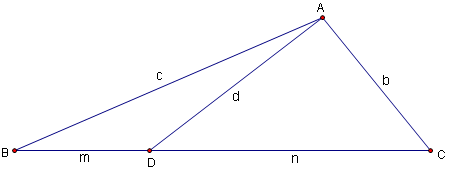
\includegraphics[width=9cm]{images/Stewarts_theorem.png}
\end{figure}

\begin{corollary}[Apollonius's Theorem (Pappus's Median Theorem)]
Given $\triangle{ABC}$. $AD$ is median from $A$ to $BC$. Then
\[AD^2=\frac{2b^2+2c^2-a^2}{4}.\]
\end{corollary}

\subsection{Ceva and Menelaus}
We will specifically look at these two theorems because they are of utmost importance in olympiad.

\begin{theorem}[Ceva's theorem] 
Given $\triangle ABC$. Point $P$ inside the triangle. Continue lines $AP$, $BP$ and $CP$ to intersect $BC$, $CA$ and $AB$ at $D$, $E$ and $F$ respectively. Then
\begin{equation}
\frac{AF}{FB}\times\frac{BD}{DC}\times\frac{CE}{EA}=1.
\end{equation} 
\end{theorem}

\begin{figure}[H]
\centering
\begin{asy}
size(6cm);
import math;
import graph;
pair A,B,C,D,E,F;
A = (0.3,0.8); B = (0,0); C = (1,0);
label("$A$",A,N);
label("$B$",B,SW);
label("$C$",C,SE);

draw(A--B--C--A);
D = (B+C)/2;
E = (A+C)/2;
F = (A+B)/2;
label("$D$",D,S);
label("$E$",E,NE);
label("$F$",F,NW);
draw(A--D);
draw(B--E);
draw(C--F);
\end{asy}
\end{figure}

\begin{theorem}[Menelaus' theorem]
Given $\triangle ABC$. A transversal intersects $BC$, $AC$ and $AB$ at points $D$, $E$ and $F$ respectively. Then we have
\begin{equation} \frac {AF}{FB} \times \frac {BD}{DC} \times \frac {CE}{EA} = 1 \end{equation} 
\end{theorem}

\begin{figure}[H]
    \centering
    \begin{tikzpicture}
    \coordinate[label=240:$C$] (C) at (0,0) {};
    \coordinate[label=below:$B$] (B) at (5,0) {};
    \coordinate[label=above:$A$] (A) at (2,4) {};
    \coordinate[label=-60:$D$] (D) at (9,0) {};
    \coordinate[label=135:$E$] (E) at (1,2) {};
    \draw (A) -- (B);
    \draw (C) -- (D);
    \draw (A) -- (C);
    \draw (D) -- (E);
    \node [label=80:$F$] at (4,1.33) {};
    \end{tikzpicture}
\end{figure}
\pagebreak

\subsection{Area of triangle}
Let $[ABC]$ denote the area of $\triangle ABC$.

\begin{proposition}
\begin{equation}
[ABC]=\frac{ah_a}{2}
\end{equation}
\end{proposition}

\begin{proposition}
\begin{equation}
[ABC]=\frac{1}{2}ab\sin C
\end{equation}
\end{proposition}

\begin{proof}
Observe that using trigonometry, we have $h_a=b\sin C$.
\end{proof}

\begin{proposition}
\begin{equation}
[ABC] = \frac{abc}{4R} 
\end{equation}
\end{proposition}

\begin{proof}
From sine rule, we have $\sin C=\dfrac{c}{2R}$. Substituting this into the above equation.
\end{proof}

\begin{proposition}
\begin{equation}
[ABC] = sr
\end{equation}
where $s$ denotes the semiperimeter, $r$ denotes the radius of incircle.
\end{proposition}

\begin{theorem}[Heron's formula]
Given $\triangle ABC$,
\begin{equation}
[ABC]=\sqrt{s(s-a)(s-b)(s-c)} 
\end{equation} 
where $s$ denotes the semiperimeter.
\end{theorem}

\begin{proof}
Our objective is to find the area of a triangle from just its three sides.

Since we know how to relate the angles of a triangle to the sides, we use $[ABC]=\frac{1}{2}ab\sin C$. Since $\sin C=\sqrt{1-\cos^2C}$, we have
\begin{align*}
[ABC] &= \frac{ab}{2}\sqrt{1-\cos^2C} \\
&= \frac{ab}{2}\sqrt{1-\frac{(c^2-a^2-b^2)^2}{4a^2b^2}} \quad \text{by cosine rule} \\
&= \sqrt{\frac{4a^2b^2-(c^2-a^2-b^2)^2}{16}} \\
&= \sqrt{\frac{(2ab-c^2+a^2+b^2)(2ab+c^2-a^2-b^2)}{16}} \\
&= \sqrt{\frac{[(a+b)^2-c^2][c^2-(a-b)^2]}{16}} \\
&= \sqrt{\frac{(a+b-c)(a+b+c)(a-b+c)(-a+b+c)}{16}} \\
&= \sqrt{s(s-a)(s-b)(s-c)}
\end{align*}
\end{proof}

\begin{equation}
[ABC]=2R^2\sin A\sin B\sin C
\end{equation}

\begin{proof}

\end{proof}

\section{Quadrilaterals}
\begin{theorem}[British flag theorem] 
If $ABCD$ is a rectangle and $P$ is a point inside of it, then we have 
\[ PA^2+PC^2=PB^2+PD^2 \] 
\end{theorem}

\begin{figure}[H]
    \centering
    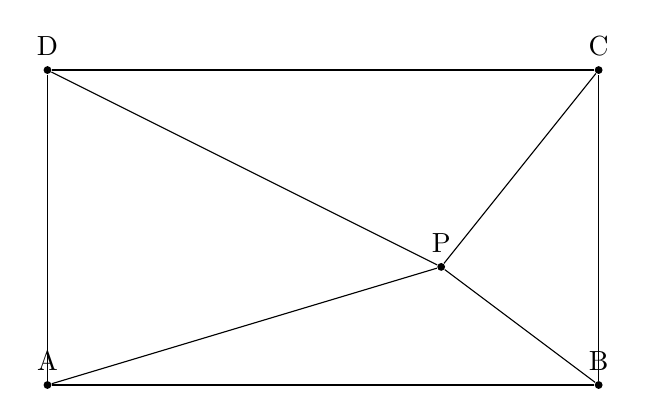
\begin{tikzpicture}[dot/.style={circle,inner sep=1pt,fill,label={#1},name=#1},
  extended line/.style={shorten >=-#1,shorten <=-#1},
  extended line/.default=1cm]
        \node [dot=A] at (0,0) {};
        \node [dot=B] at (7,0) {};
        \node [dot=C] at (7,4) {};
        \node [dot=D] at (0,4) {};
        \node [dot=P] at (5,1.5) {};
        \draw (A) -- (B) -- (C) -- (D) -- (A);
        \draw (P) -- (A);
        \draw (P) -- (B);
        \draw (P) -- (C);
        \draw (P) -- (D);
    \end{tikzpicture}
\end{figure}

\begin{proof}
This can be easily proven using Pythagoras' Theorem.
\end{proof}
\pagebreak

\section{Circle}
% https://yufeizhao.com/olympiad/cyclic_quad.pdf
The reader should be familiar with basic circle terminology, such as \vocab{centre}, \vocab{radius}, \vocab{chord}, \vocab{diameter}, \vocab{tangent}, \vocab{secant}, \vocab{arc}, \vocab{sector}, \vocab{segment}, and \vocab{circumference}.

\subsection{Angles}
\begin{itemize}
\item Angle subtended at the centre of a circle by a chord is twice the angle subtended on the circumference.
\item All angles subtended by a fixed chord in the same segment of a circle are equal.
\end{itemize}

\subsection{Cyclic Quadrilaterals}
Unlike triangles, not all quadrilaterals can be inscribed in a circle. Those which can be are known as \vocab{cyclic quadrilaterals}. Such quadrilaterals have the following special properties:
\begin{itemize}
\item Sum of opposite angles in a cyclic quadrilaterals is always $180\degree$.
\item When we draw the diagonals of a cyclic quadrilaterals, we form four pairs of equal inscribed angles.
\end{itemize}

% AOPS book 2 - Chapter 4 (pg 33)

Angle chasing and cyclic quadrilaterals
\begin{theorem}[Ptolemy's theorem]
Given a cyclic quadrilateral $ABCD$, the product of lengths of diagonals is equal to the sum of products of lengths of the pairs of the opposite sides: 
\begin{equation}
AC \cdot BD = AB \cdot CD + AD \cdot BC 
\end{equation} 
\end{theorem}

\begin{figure}[H]
\centering
\begin{asy}
import graph; size(6cm); real lsf=0.5; real xmin=-12.650403526770004,xmax=10.832004349475627,ymin=-7.279059049128651,ymax=2.9172496339779594; 
pair A=(-4.722835236346583,1.9593464813112522), B=(-0.13581566098455275,2.055853491787133), C=(1.9952034907831915,-3.715500660891391), D=(-6.4478295435721815,-4.230092924079331); 
draw(A--B--C--D--cycle); 
draw(A--C); draw(B--D);
draw(circle((-2.3441952074649755,-2.0386768685399885),4.652109101574643));
label("$A$",A,NW*lsf); label("$B$",B,NE*lsf); label("$C$",C,SE*lsf); label("$D$",D,SW*lsf); 
clip((xmin,ymin)--(xmin,ymax)--(xmax,ymax)--(xmax,ymin)--cycle);  
\end{asy}
\end{figure}

\begin{theorem}[Ptolemy's inequality]
For four points $A, B, C, D$ in the plane,
\begin{equation}
AB \cdot CD + BC \cdot DA \ge AC \cdot BD
\end{equation}
where equality holds if and only if $ABCD$ is a cyclic quadrilateral with diagonals $AC$ and $BD$ (or a trivial case where $A$, $B$, $C$ and $D$ are collinear.
\end{theorem}

\begin{proof}
We construct a point $P$ such that the triangles $APB$ and $DCB$ are similar and have the same orientation. This means that
\begin{equation} \tag{1}
BD = \frac{BA \cdot DC}{AP}
\end{equation}

But since this is a spiral similarity, we also know that the triangles $ABD$ and $PBC$ are also similar, which implies that
\begin{equation} \tag{2}
BD = \frac{BC \cdot AD}{PC}
\end{equation}

By the triangle inequality, we have $AP + PC \ge AC$. Multiplying both sides of the inequality by $BD$ and using equations $(1)$ and $(2)$ gives us
\[ BA \cdot DC + BC \cdot AD \ge AC \cdot BD \]

which is the desired inequality. Equality holds iff $A$, $P$, $C$ are collinear. But since the triangles $BAP$ and $BDC$ are similar, this would imply that the angles $BAC$ and $BDC$ are congruent, i.e. that $ABCD$ is a cyclic quadrilateral.
\end{proof}

\begin{theorem}[Brahmagupta's formula] 
Given a cyclic quadrilateral $ABCD$, 
\begin{equation}
[ABCD]=\sqrt{(s-a)(s-b)(s-c)(s-d)} 
\end{equation}
where $s$ denotes the semiperimeter.
\end{theorem}
\pagebreak

\subsection{Power of a Point} % https://cs.stanford.edu/~rayyli/static/contest/lectures/Ray%20Li%20pop.pdf
\textbf{Power of a point} is a frequently used tool in Olympiad geometry.

\begin{theorem}[Power of a point]
Let $\Gamma$ be a circle, and $P$ be a point. Let a line through $P$ meet $\Gamma$ at points $A$ and $B$, and another line through $P$ meet $\Gamma$ at points $C$ and $D$. Then 
\begin{equation}
PA \cdot PB = PC \cdot PD
\end{equation} 
\end{theorem}

\begin{figure}[H]
    \centering
    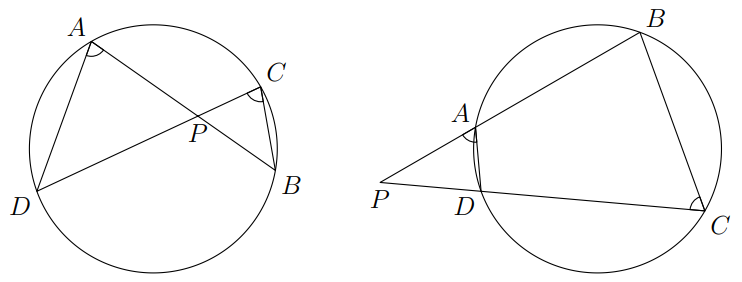
\includegraphics[width=12cm]{images/Power_of_a_point.png}
\end{figure}

\begin{proof}
There are two configurations to consider, depending on whether $P$ lies inside the circle or outside the circle.

When $P$ lies inside the circle, we have $\angle PAD = \angle PCB$ and $\angle APD = \angle CPB$, so triangles $PAD$ and $PCB$ are similar. Hence $\dfrac{PA}{PD} = \dfrac{PC}{PB}$. Rearranging, we get $PA \cdot PB = PC \cdot PD$.

When $P$ lies outside the circle, we have $\angle PAD = \angle PCB$ and $\angle APD = \angle CPB$, so again triangles $PAD$ and $PCB$ are similar. We get the same result in this case.
\end{proof}

As a special case, when $P$ lies outside the circle and $C=D$ ($PC$ is a tangent), we have \begin{equation} PA \cdot PB = PC^2 \end{equation}

\begin{figure}[H]
    \centering
    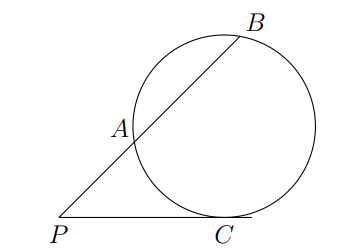
\includegraphics[width=6cm]{images/Power_of_a_point2.png}
\end{figure}
\pagebreak

\begin{theorem}[Converse to power of a point]
Let $A, B, C, D$ be four distinct points. Let lines $AB$ and $CD$ intersect at $P$. Assume that either (1) $P$ lies on both line segments $AB$ and $CD$, or (2) $P$ lies on neither line segments. Then $A, B, C, D$ are concyclic if and only if $PA \cdot PB = PC \cdot PD$.
\end{theorem}

\begin{proof}
The expression $PA \cdot PB = PC \cdot PD$ can be rearranged as $\dfrac{PA}{PD} = \dfrac{PC}{PB}$. In both configurations described in the statement of the theorem, we have $\angle APD = \angle CPB$. It follows by angles and ratios that triangles $APD$ and $CPB$ are similar.

Thus $\angle PAD = \angle PCB$. In both cases this implies that $A$, $B$, $C$ and $D$ are concyclic.
\end{proof}

\begin{definition}
Suppose that $\Gamma$ has centre $O$ and radius $r$. We say that the \vocab{power} of point $P$ with respect to $\Gamma$ is
\[ OP^2-r^2. \]
\end{definition}

Let line $PO$ meet $\Gamma$ at points $A$ and $B$, so that $AB$ is a diameter. We will use \emph{directed lengths}, meaning that for collinear points $P, A, B$, an expression such as $PA \cdot PB$ is assigned a positive value if $PA$ and $PB$ point in the same direction, and a negative value if they point in opposite directions. Then
\[ PA \cdot P B = (PO + OA)(PO + OB) = (PO-r)(PO+r) = PO^2-r^2, \]
which is the power of $P$. So the power of a point theorem says that this quantity equals to $PC \cdot PD$, where $C$ and $D$ are the intersections with $\Gamma$ of any line through $P$.

By convention, the power of $P$ is negative when $P$ is inside the circle, and positive when $P$
is outside the circle. When $P$ is outside the circle, the power equals to the square of the length
of the tangent from $P$ to the circle.

\begin{figure}[H]
    \centering
    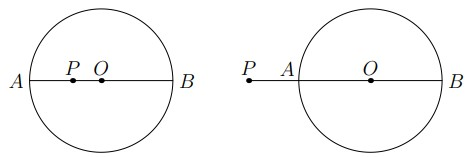
\includegraphics[width=8cm]{images/Power_of_a_point3.jpg}
\end{figure}

Let $\Gamma_1$ and $\Gamma_2$ be two circles with different centres $O_1$ and $O_2$, and radii $r_1$ and r$_2$ respectively.

\begin{definition}
The \vocab{radical axis} of $\Gamma_1$ and $\Gamma_2$ is the set of points with equal powers with respect to both circles.
\[ {PO_1}^2-{r_1}^2 = {PO_2}^2-{r_2}^2 \]
which can be represented as 
\[ pow(P, \Gamma_1) = pow(P, \Gamma_2). \]
\end{definition}

\begin{lemma}
The radical axis is a line perpendicular to the line connecting the circles' centres.
\end{lemma}

\begin{proof}
We first prove two lemmas.
\begin{lemma}
Let $P$ be a point in the plane, and let $P'$ be the foot of the perpendicular from $P$ to $O_1O_2$. Then \[ pow(P, \Gamma_1)-pow(P, \Gamma_2) = pow(P', \Gamma_1)-pow(P', \Gamma_2). \]
\end{lemma}
The proof of the lemma is an easy application of the Pythagorean Theorem.

\begin{lemma}
There is a unique point $P$ on line $O_1O_2$ such that $pow(P, O_1) = pow(P, O_2)$.
\end{lemma}

Proof: First show that $P$ lies between $O_1$ and $O_2$ via proof by contradiction, by using a bit of inequality theory and the fact that $O_1O_2 > r_1 + r_2$. Then, use the fact that $O_1P + PO_2 = O_1O_2$ (a constant) to prove the lemma.

The first lemma shows that every point on the plane can be equivalently mapped to a line on $O_1O_2$. The second lemma shows that only one point in this mapping satisfies the given condition. Combining these two lemmas shows that the radical axis is a line perpendicular to $\ell$, hence proved.
\end{proof}

When $\Gamma_1$ and $\Gamma_2$ intersect, the intersection points $A$ and $B$ both have a power of $0$ with respect to either circle, so $A$ and $B$ must lie on the radical axis. This shows that the radical axis \emph{coincides with the common chord} when the circles intersect.

To show that some point lies on the radical axis or the common chord, we can show that the point has \emph{equal powers with respect to the two circles}.

\begin{figure}[H]
    \centering
    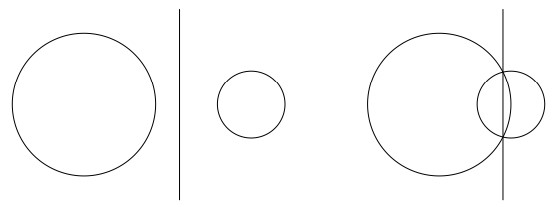
\includegraphics[width=10cm]{images/Radical_axis.jpg}
    \caption{Radical axis}
\end{figure}

\begin{figure}[H]
    \centering
    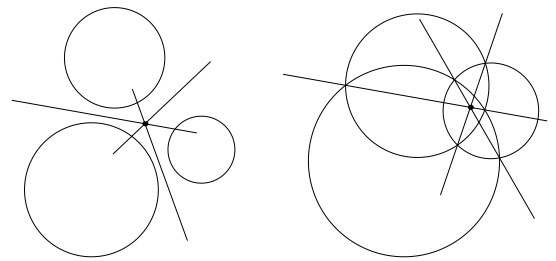
\includegraphics[width=10cm]{images/Radical_center.jpg}
    \caption{Radical centre}
\end{figure}

\begin{theorem}[Radical axis theorem]
Given three circles, no two concentric, the three pairwise radical axes (which are non-parallel) are concurrent, at a point known as the radical centre.
\end{theorem}

\begin{proof}
Denote the three circles by $\Gamma_1, \Gamma_2, \Gamma_3$, and denote the radical axes of $\Gamma_i$ and $\Gamma_j$ by $\ell_{ij}$.

Suppose that the radical axes are not all parallel. Let $\ell_{12}$ and $\ell_{13}$ meet at $X$. Since $X$ lies on $\ell_{12}$, it has equal powers with respect to $\Gamma_1$ and $\Gamma_2$. Since X lies on $\ell_{13}$, it has equal powers with respect to $\Gamma_1$ and $\Gamma_3$. Therefore, $X$ has equal powers with respect to all three circles, and hence it must lie on $\ell_{23}$ as well.
\end{proof}

\subsection{Theorems}
\begin{theorem}[Hamilton's theorem]
For $\triangle ABC$ with circumcentre $O$ and orthocentre $H$,
\[ \overrightarrow{OH} = \overrightarrow{OA} + \overrightarrow{OB} + \overrightarrow{OC} \]
\end{theorem}

\begin{theorem}[Euler line]
Circumcentre $O$, the centroid $G$ and the orthocentre $H$ are collinear. We also have
\[GH=2OG\]
and
\[OI^2=R^2-2Rr.\]
\end{theorem}

\begin{figure}[H]
\centering
\begin{asy}
import graph; size(8cm); real lsf=0.5; pen dps=linewidth(0.7)+fontsize(10); defaultpen(dps); pen ds=black; real xmin=-10.190749488267803,xmax=2.1327044306677894,ymin=-5.404837089903882,ymax=2.8163349988738835; 
pair A=(-5.649772389356279,1.9593464813112522), B=(-7.46244948857524,-2.6753392837372125), C=(-0.42710735249361875,-2.0393655406135887), G=(-4.513109743475047,-0.9184527810131827), H=(-5.466468833129196,-0.06841527263166719), O=(-4.03643019864797,-1.3434715352039406); 
draw(A--B--C--cycle);  draw(circle((-4.036430198647971,-1.3434715352039408),3.675796495256074)); draw((xmin,-0.8916236469616956*xmin-4.942448149628765)--(xmax,-0.8916236469616956*xmax-4.942448149628765),red); 
label("$A$",A,N*lsf); label("$B$",B,SW*lsf); label("$C$",C,E*lsf); dot(G,linewidth(4.pt)+ds); label("$G$",G,NE*lsf); dot(H,linewidth(4.pt)+ds); label("$H$",H,NE*lsf); dot(O,linewidth(4.pt)+ds); label("$O$",O,NE*lsf); 
clip((xmin,ymin)--(xmin,ymax)--(xmax,ymax)--(xmax,ymin)--cycle);  
\end{asy}
\end{figure}

\begin{theorem}[Nine-point circle]
The midpoints of each side of the triangle, the feet of each altitude, and the midpoints of the line segments from each vertex to the orthocentre, all lie on a single circle.
\end{theorem}

The centre of this circle lies on the Euler line, at the midpoint between the orthocentre and circumcentre.

The radius of this circle is half the circumradius of the triangle.

\begin{figure}[H]
\centering
\begin{asy}
import graph; size(8cm); real lsf=0.5; pen ds=black; real xmin=-9.29991987799322,xmax=4.227854476335946,ymin=-2.582016893191067,ymax=3.3073835513057874; 
pair A=(-4.3010727599189025,2.646623812442647), B=(-6.237341479539152,-1.782075918603663), C=(1.0133669173366817,-1.8026745220038782), D=(-4.313669818746617,-1.787540894912733), F=(-5.081333386332044,0.8619851456466379), G=(-2.6119872811012352,-1.7923752203037706), H=(-1.6438529212911104,0.4219746452193843), I=(-5.269207119729027,0.43227394691949195); 
draw(A--B--C--cycle); 
draw(A--D); draw(B--(-3.2595890330248367,1.7746839480662215)); draw(C--F); draw(circle((-3.458037931575361,-0.10366039891128645),1.8887984146430965),red); 
label("$A$",A,N*lsf); label("$B$",B,SW*lsf); label("$C$",C,SE*lsf); dot(D,ds); label("$D$",D,SW*lsf); dot((-3.2595890330248367,1.7746839480662215),ds); label("$E$",(-3.2595890330248367,1.7746839480662215),NE*lsf); dot(F,ds); label("$F$",F,NW*lsf); dot(G,ds); label("$G$",G,SE*lsf); dot(H,ds); label("$H$",H,NE*lsf); dot(I,ds); label("$I$",I,W*lsf); 
clip((xmin,ymin)--(xmin,ymax)--(xmax,ymax)--(xmax,ymin)--cycle); 
\end{asy}
\end{figure}

\begin{theorem}[Simson line]
Let $P$ be a point on the circumcircle of $\triangle ABC$. Points $D,E,F$ are the feet of the perpendicular bisectors from $P$ to sides (or the extensions of) $AB,AC,BC$ respectively. Then $D,E,F$ are collinear.
\end{theorem}

\begin{figure}[H]
\centering
\begin{asy}
import graph; size(8cm); real lsf=0.5; pen ds=black; real xmin=-11.67954538469208,xmax=9.668098139167585,ymin=-4.858791244160047,ymax=4.410580285936885;
pair A=(-3.0618387621655723,3.2139886884152817), B=(-5.142297705587335,-1.379499869832753), C=(1.7170372266844143,-1.338302663032322), P=(-1.8556455955550775,-3.79185012983495), D=(-5.489473189178031,-2.1460358385528), F=(-1.8702522152840195,-1.3598479449660663); 
draw(A--B--C--cycle); 
draw(circle((-1.71982057252597,-0.16171080952667127),3.6326794410915353)); draw(B--D,dashed); draw(P--D); draw(P--F); draw(P--(1.0693209211634036,-0.7212970444110164)); draw(D--(1.0693209211634036,-0.7212970444110164),red); 
label("$A$",A,N*lsf); label("$B$",B,W*lsf); label("$C$",C,E*lsf); dot(P,ds); label("$P$",P,S*lsf); dot(D,ds); label("$D$",D,W*lsf); dot((1.0693209211634036,-0.7212970444110164),ds); label("$E$",(1.0693209211634036,-0.7212970444110164),NE*lsf); dot(F,ds); label("$F$",F,N*lsf); 
clip((xmin,ymin)--(xmin,ymax)--(xmax,ymax)--(xmax,ymin)--cycle);  
\end{asy}
\end{figure}

\begin{proof}
Proof of existence: It suffices to show that $\angle NMP+\angle PML=180\degree$. 

$PCAB$ is a cyclic quadrilateral, so $\angle PBA+\angle ACP=\angle PBN+\angle ACP=180\degree$. $PMNB$ is a cyclic quadrilateral (since $\angle PMB=\angle PNB=90\degree$), so $\angle PBN+\angle NMP=180\degree$. Hence $\angle NMP=\angle ACP$. Now $PLCM$ is cyclic, so $\angle PML=\angle PCL=180\degree-\angle ACP$.

Therefore $\angle NMP+\angle PML=\angle ACP+(180\degree-\angle ACP)=180\degree$.
\end{proof}

We now prove some properties regarding the Simson line.

The Simson line of a vertex of the triangle is the altitude of the triangle dropped from that vertex, and the Simson line of the point diametrically opposite to the vertex is the side of the triangle opposite to that vertex.
If P and Q are points on the circumcircle, then the angle between the Simson lines of P and Q is half the angle of the arc PQ. In particular, if the points are diametrically opposite, their Simson lines are perpendicular and in this case the intersection of the lines lies on the nine-point circle.

\begin{lemma}
Let $ABC$ be a triangle with orthocentre $H$ and circumcircle $\odot(ABC)$. Suppose $P\in\odot(ABC)$. Let $\gamma$ be Simson's line of $P$ wrt $ABC$.

Prove that $\gamma$ bisects $PH$.
\end{lemma}

\begin{proof}
Let $PA,PB,PC$ be the projections of $P$ on the sides $BC,AC,AB$; let $Q$ be the intersection between $AH$ and the Simson's line of $P$. We want to show that $HQ=PP_A$. If we call $H_A$ the symmetric of $H$ with respect to the $BC$ side, we have that $HA$ lies on the circumcircle of $ABC$, so, in order to prove that $HQ=PP_A$, it is sufficient to show that $PP_AQH_A$ is an isosceles trapezoid. Let $\theta=\widehat{P_C P_A B}=\widehat{P_B P_A C}$. Since $PP_AP_CB$ and $PP_ACP_B$ are cyclic quadrilaterals, we have $\theta=\widehat{P_C P B}=\widehat{P_B P C}$, too.

Now:
\[\widehat{P_A Q H_A}=\frac{\pi}{2}-\theta,\]
and:
\[\widehat{P H_A Q}=\widehat{P H_A A}=\widehat{P B A}=\widehat{P B P_C}=\frac{\pi}{2}-\theta.\]
Since $PP_A$ and $QH_A$ are both ortogonal to $BC$, $PP_AQH_A$ is an isosceles trapezoid and we have $PP_A=QH$.
\end{proof}

Given two triangles with the same circumcircle, the angle between the Simson lines of a point P on the circumcircle for both triangles does not depend of P.

\begin{theorem}[Miquel's theorem]
Let $ABC$ be a triangle, and let $X, Y, Z$ be points on lines $BC, CA, AB$ respectively. Assume that the six points $A, B, C, X, Y, Z$ are all distinct. Then the circumcircles of triangles $AYZ, BZX, CXY$ pass through a common point.
\end{theorem}

\begin{figure}[H]
\centering
\begin{asy}
import graph; size(8cm); real lsf=0.5; pen ds=black; real xmin=-10.647193519393634,xmax=4.272620939998431,ymin=-3.1737370566747436,ymax=3.3046034322717803; 
pair A=(-4.681638029546153,2.7008962037190067), B=(-6.535512335565544,-1.7072049239270888), C=(-0.08814947129810388,-1.666007717126658), X=(-5.45557620465073,0.8606432095814611), Y=(-2.506653486956552,0.6331978941719494), Z=(-3.2603364974088445,-1.6862772827887074), D=(-3.2431897895257977,-0.11518658185591212); 
draw(A--B--C--cycle); 
draw(circle((-3.93804793471393,1.3053008916287092),1.5813325090761299)); draw(circle((-4.903125898654128,-0.8827091442329125),1.8287916147406886)); draw(circle((-1.6790880103434862,-0.9178959325207675),1.758054799284159)); 
label("$A$",A,N*lsf);label("$B$",B,SW*lsf); label("$C$",C,SE*lsf); label("$X$",X,W*lsf); label("$Y$",Y,NE*lsf); label("$Z$",Z,S*lsf); dot(D,ds); label("$D$",D,N*lsf); 
clip((xmin,ymin)--(xmin,ymax)--(xmax,ymax)--(xmax,ymin)--cycle); 
\end{asy}
\end{figure}

\begin{proof}
The proof involves angle chasing.
\end{proof}

Generalising, the circumcircles of the four triangles in a cyclic quadrilateral are concurrent.
\pagebreak

\section*{Exercises}
\begin{prbm}[\acrshort{smo} Open 2005 Q2]
Circles $C_1$ and $C_2$ have radii $3$ and $7$ respectively. The circles intersect at distinct points $A$ and $B$. A point $P$ outside $C_2$ lies on the line determined by $A$ and $B$ at a distance of $5$ from the center of $C_1$. Point $Q$ is chosen on $C_2$ so that $PQ$ is tangent to $C_2$ at $Q$. Find the length of the segment $PQ$.
\end{prbm}

\begin{solution}
The point $P$ lies on the radical axis of $C_1$ and $C_2$, namely $AB$, and hence has equal power with respet to both circles. Thus $PQ^2=5^2-3^2=16$.
\end{solution}
\pagebreak

\begin{prbm}[\acrshort{smo} Open 2005 Q10]
It is known that the three sides of a triangle are consecutive positive integers and the largest angle is twice the smallest angle. Find the perimeter of this triangle.
\end{prbm}

\begin{solution}
Let $\angle C=2\angle A$ and $CD$ the bisector of $\angle C$. Let $BC=x-1$, $CA=x$, $AB=x+1$. Then $\triangle ABC\sim\triangle CBD$, which implied
\[ \frac{BD}{BC}=\frac{BC}{AB}\implies BD=\frac{(x-1)^2}{x+1} \]
and
\[ \frac{CD}{AC}=\frac{CB}{AB}\implies AD=CD=\frac{x(x-1)}{x+1}. \]
Since $AB=AD+BD$, we have
\[ \frac{x(x-1)}{x+1}+\frac{(x-1)^2}{x+1}=x+1. \]
The only positive solution to this equation is $x=5$. Hence the perimeter is $15$.
\end{solution}
\pagebreak

\begin{prbm}[\acrshort{mat} 2022]
100 circles all share the same centre, the $n$-th circle named as $C_n$. For each whole number $n$ between 1 and 99 inclusive, a tangent to circle $C_n$ intersects circle $C_{n+1}$ at two points, separated by a distance of 2.

Given that $C_1$ has radius 1, what is the radius of $C_{100}$?
\end{prbm}

\begin{solution}
The relationship between circle $C_n$ of radius $r_n$ and circle $C_{n+1}$ of radius $r_{n+1}$ is shown below.

\begin{figure}[H]
\centering
\begin{asy}
size(6cm);
draw(circle((0,0),5));
draw(circle((0,0),3));
dot((0,0));
dot((3,4));
draw((0,0)--(3,4));
label("$r_{n+1}$",(0,0)--(3,4),NW);
dot((3,0));
draw((0,0)--(3,0));
label("$r_n$",(0,0)--(3,0),S);
draw((3,4)--(3,-4));
label("$1$",(3,4)--(3,0),E);
label("$1$",(3,-4)--(3,0),E);
\end{asy}
\end{figure}

The tangent is perpendicular to the radius, so there is a right-angled triangle with hypotenuse $r_{n+1}$ and other sides $r_n$ and $1$. By Pythagoras, we have 
\[ {r_{n+1}}^2 = {r_n}^2 + 1. \]
Since ${r_1}^2 = 1$, we have ${r_2}^2 = 2$ and ${r_3}^2 = 3$ and so on, up to ${r_{100}}^2 = 100$, so the radius of $C_{100}$ is 10.
\end{solution}
\pagebreak

\begin{prbm}[\acrshort{tstst} P5]
Let $ABC$ be a triangle with incentre $I$. Let $D$ be a point on side $BC$ and let $\omega_B$ and $\omega_C$ be the incircles of $\triangle ABD$ and $\triangle ACD$, respectively. Suppose that $\omega_B$ and $\omega_C$ are tangent to segment $BC$ at points $E$ and $F$, respectively. Let $P$ be the intersection of segment $AD$ with the line joining the centers of $\omega_B$ and $\omega_C$. Let $X$ be the intersection point of lines $BI$ and $CP$ and let $Y$ be the intersection point of lines $CI$ and $BP$. Prove that lines $EX$ and $FY$ meet on the incircle of $\triangle ABC$.
\end{prbm}

\begin{solution}
(homothety): Let $Z$ be the diametrically opposite point on the incircle. We claim this is the desired intersection.

\begin{figure}[H]
\centering
\begin{asy}
import geometry; import graph; import olympiad;

size(8cm); pair A = dir(110); pair B = dir(210); pair C = dir(330);

draw(A--B--C--cycle,red); draw(incircle(A, B, C),  lightblue);

pair D = 0.35*B+0.65*C; draw(A--D, red);

pair I_B = incentre(A, B, D); pair I_C = incentre(A, C, D); pair E = foot(I_B, B, C); pair F = foot(I_C, B, C);

draw(incircle(A, B, D), heavygreen); draw(incircle(A, C, D), heavygreen); pair I = incentre(A, B, C);

pair P = extension(I_B, I_C, A, D); draw(I_B--I_C, heavygreen);

pair X = extension(B, I, C, P); pair Y = extension(C, I, B, P); pair Z = extension(E, X, F, Y); draw(B--I--C, red); draw(X--C, dotted+heavygreen); draw(Y--B, dotted+heavygreen); draw(E--Z--F, dashed+heavygreen);

pair T = extension(B, C, I_B, I_C); draw(I_C--T, dotted+heavygreen); draw(C--T, dotted+red); pair W = foot(I, B, C);

dot("$A$", A, dir(A)); dot("$B$", B, dir(270)); dot("$C$", C, dir(270)); dot("$D$", D, dir(D)); dot("$I_B$", I_B, dir(170)); dot("$I_C$", I_C, dir(30)); dot("$E$", E, dir(E)); dot("$F$", F, dir(F)); dot("$I$", I, dir(90)); dot("$P$", P, dir(250)); dot("$X$", X, dir(160)); dot("$Y$", Y, dir(20)); dot("$Z$", Z, dir(140)); dot("$T$", T, dir(T)); dot("$W$", W, dir(W));
\end{asy}
\end{figure}

Note that:
$P$ is the insimilicenter of $\omega_B$ and $\omega_C$
$C$ is the exsimilicenter of $\omega$ and $\omega_C$.
Thus by Monge theorem, the insimilicenter of $\omega_B$ and $\omega$ lies on line $CP$.

This insimilicenter should also lie on the line joining the centers of $\omega$ and $\omega_B$, which is $\overline{BI}$, hence it coincides with the point $X$. So $X \in \overline{EZ}$ as desired.
\end{solution}

\begin{solution}
(harmonic): Let $T = \overline{I_B I_C} \cap \overline{BC}$, and $W$ the foot from $I$ to $\overline{BC}$. Define $Z = \overline{FY} \cap \overline{IW}$. Because $\angle I_B D I_C = 90^{\circ}$, we have\[ -1 = (I_B I_C; PT) \overset{B}{=} (I I_C; YC) 	\overset{F}{=} (I\infty; ZW) \]So $I$ is the midpoint of $\overline{ZW}$ as desired.
\end{solution}

\begin{solution}
(outline, barycentric, Andrew Gu): Let $AD = t$, $BD = x$, $CD = y$ (so with Stewart). We then have $D = (0:y:x)$ and so\[ \overline{AI_B} \cap \overline{BC} = \left( 0 : y + \frac{tx}{c+t} : \frac{cx}{c+t} \right) \]hence intersection with $BI$ gives $I_B = (ax : cy+at : cx)$. Similarly, $I_C = (ay : by : bx+at)$.

Then, we can compute\[ P = \left( 2axy : y(at+bx+cy) : x(at+bx+cy) \right) \]since $P \in \overline{I_B I_C}$, and clearly $P \in \overline{AD}$. Intersection now gives\begin{align*} 	X &= \left( 2ax : at+bx+cy : 2cx \right) \\ 	Y &= \left( 2ay : 2by : at+bx+cy \right). \end{align*}From here one can check that the antipode\[ Q = \left( 4a^2 : -a^2+2ab-b^2+c^2 : -a^2+2ac-c^2+b^2 \right) \]lies on each of lines $EX$ and $FY$ (using Stewart's Theorem).
\end{solution}
\pagebreak

\begin{prbm}[\acrshort{australia} 2024 P2]
Let $ABCD$ be a cyclic quadrilateral. Point $P$ is on line $CB$ such that $CP=CA$and $B$ lies between $C$ and $P$. Point $Q$ is on line $CD$ such that $CQ=CA$ and $D$ lies between $C$ and $Q$. Prove that the incentre of triangle $ABD$ lies on line $PQ$.
\end{prbm}

\begin{proof}
Let $PQ$ intersect the angle bisector of $\angle{BAC}$ at $I'$. $APBI'$ is cyclic since $\angle{BPI'}=\frac{\angle{A}}{2}=\angle{PAI'}$. Then, $\angle{I'BA}=\angle{I'PA}=\frac{\angle{QCA}}{2}=\frac{\angle{B}}{2}$ so $I'=I$ and we are done.
\end{proof}

\chapter{Analytic Geometry}
\section{Trigonometry}
% https://www.ams.org/books/prb/025/prb025-endmatter.pdf
% https://mathematicalolympiads.files.wordpress.com/2012/08/103-trigonometry-problems-titu-andreescu-zuming-feng.pdf
\vocab{Trigonometric functions} describe how the ratio of lengths vary according to the angle between the lengths.

For a triangle $\triangle ABC$ with $\angle C=90\degree$, we define \vocab{sine} as
\begin{equation}
\sin A=\frac{a}{c}
\end{equation}
and \vocab{cosine} as
\begin{equation}
\cos A=\frac{b}{c}.
\end{equation}
We define \vocab{tangent} as the ratio of sine and cosine; that is,
\begin{equation}
\tan A=\frac{\sin A}{\cos A}=\frac{a}{b}.
\end{equation}
We also define the reciprocals of the above trigonometric functions: \vocab{cosecant}, \vocab{secant} and \vocab{cotangent} are the reciprocals of sine, cosine and tangent respectively.
\begin{equation}
\cosec A=\frac{1}{\sin A}
\end{equation}
\begin{equation}
\sec A=\frac{1}{\cos A}
\end{equation}
\begin{equation}
\cot A=\frac{1}{\tan A}
\end{equation}

\subsection{Pythagorean identities}
The following equation is known as the \vocab{Pythagorean identity}.
\begin{equation}\label{pythagorean_identity}
\sin^2 A + \cos^2 A = 1
\end{equation}
\begin{proof}
\[ \sin^2A+\cos^2A=\brac{\frac{a}{c}}^2+\brac{\frac{b}{c}}^2=\frac{a^2+b^2}{c^2} \]
By Pythagoras' Theorem, for a right-angled triangle, $a^2+b^2=c^2$. Hence we have our desired result.
\end{proof}
The following two equations are corollaries of \cref{pythagorean_identity}; they can be easily derived and shall be left as an exercise for the reader.
\[ \tan^2 A + 1 = \sec^2 A \]
\[ 1 + \cot^2 A = \cosec^2 A \]

\begin{exercise}
Compute $\sin^25\degree+\sin^210\degree+\cdots+\sin^290\degree$.
\end{exercise}
\begin{solution}
\begin{align*}
&\sin^25\degree+\sin^210\degree+\cdots+\sin^290\degree \\
&= (\sin^25\degree+\sin^285\degree) + \cdots + (\sin^240\degree+\sin^250\degree)+\sin^245\degree+\sin^290\degree \\
&= (\sin^25\degree+\cos^25\degree) + \cdots + (\sin^240\degree+\cos^240\degree)+\frac{1}{2}+1 \\
&= 8(1)+\frac{1}{2}+1 \\
&= \boxed{9\frac{1}{2}}
\end{align*}
\end{solution}

\begin{exercise}
Evaluate
\[ \tan10\degree\tan20\degree\tan30\degree\cdots\tan80\degree. \]
\end{exercise}
\begin{solution}
Writing this in terms of sines and cosines, we have
\[ \frac{\sin10\degree\sin20\degree\sin30\degree\cdots\sin80\degree}{\cos10\degree\cos20\degree\cos30\degree\cdots\cos80\degree}. \]
Applying $\sin x=\cos(90\degree-x)$ to each term in the numerator, we get
\[ \frac{\cos80\degree\cos70\degree\cos60\degree\cdots\cos10\degree}{\cos10\degree\cos20\degree\cos30\degree\cdots\cos80\degree}=\boxed{1} \]
\end{solution}

\subsection{Addition formulae}
\[ \sin (A \pm B) = \sin A \cos B \pm \cos A \sin B \]
\[ \cos (A \pm B) = \cos A \cos B \mp \sin A \sin B \]
\[ \tan (A \pm B) = \frac{\tan A \pm \tan B}{1 \mp \tan A \tan B} \]

\subsubsection{Double-angle formulae}
\[ \sin 2A = 2 \sin A \cos A \]
\[ \begin{split}
\cos 2A &= \cos^2 A-\sin^2 A \\
&= 2 \cos^2 A-2 \\
&= 2-2 \sin^2 A
\end{split} \]
\[ \tan 2A = \frac{2 \tan A}{1-\tan^2 A} \]

\subsubsection{Triple-angle formulae}
\[ \sin 3A = 3 \sin A-4 \sin^3 A \]
\[ \cos 3A = 4 \cos^3 A- 3 \cos A \]
\[ \tan 3A = \frac{3\tan A-\tan^3A}{1-3\tan^2A} \]

\subsubsection{Half-angle formulae}
The following formulae are corollaries of the double angle formulae:
\[ \sin \frac{A}{2} = \pm \sqrt{\frac{1-\cos A}{2}} \]
\[ \cos \frac{A}{2} = \pm \sqrt{\frac{1+\cos A}{2}} \]

\subsubsection{Multiple-angle formulae}
To generalise, multiple-angle formulae are given by
\[ \sin nA = \sum_{k=0}^n \binom{n}{k} \cos^kA \sin^{n-k}A \sin\frac{n-k}{2}\pi \]
\[ \cos nA = \sum_{k=0}^n \binom{n}{k} \cos^kA \sin^{n-k}A \cos\frac{n-k}{2}\pi \]

\subsubsection{Sum to product}
The sum-to-product formulae can be derived from the addition formulae.
\[ \sin A + \sin B = 2 \sin \frac{A+B}{2} \cos \frac{A-B}{2} \]
\[ \sin A-\sin B = 2 \cos \frac{A+B}{2} \sin \frac{A-B}{2} \]
\[ \cos A + \cos B = 2 \cos \frac{A+B}{2} \cos \frac{A-B}{2} \]
\[ \cos A-\cos B = -2 \sin \frac{A+B}{2} \sin \frac{A-B}{2} \]

\subsubsection{Product to sum}
The product-to-sum formulae can be, in turn, simply observed from the sum-to-product formulae.
\[ \sin A \cos B = \frac{1}{2}\sqbrac{\sin(A+B)+\sin(A-B)} \]
\[ \cos A\sin B=\frac{1}{2}\sqbrac{\sin(A+B)-\sin(A-B)} \]
\[ \cos A\cos B = \frac{1}{2}\sqbrac{\cos(A+B)+\cos(A-B)} \]
\[ \sin A\sin B = -\frac{1}{2}\sqbrac{\cos(A+B)-\cos(A-B)} \]

\subsection{R-formula}
It is rather difficult to immediately the amplitude of some function of a combination of trigonometric functions, given by $f(x)=a\sin\theta+b\cos\theta$. To do so, we combine the two trigonometric functions using the \vocab{R-formula}.
\[ a \sin \theta \pm b \cos \theta = \sin (\theta \pm \alpha) \]
\[ a \cos \theta \mp b \cos \theta = \cos (\theta \pm \alpha) \]
where $R = \sqrt{a^2 + b^2}$,
$\alpha = \tan^{-1} \dfrac{b}{a}$ where $0 < \alpha < \frac{\pi}{4}$.

\subsection{Sine and Cosine Rules}
\begin{theorem}[Sine rule] 
Given $\triangle ABC$,
\begin{equation}
\frac{a}{\sin A}=\frac{b}{\sin B}=\frac{c}{\sin C}=2R
\end{equation} 
where $R$ denotes the circumradius of $\triangle ABC$.
\end{theorem}

\begin{theorem}[Cosine rule]
Given $\triangle ABC$,
\begin{equation}
c^2=a^2+b^2-2ab\cos C
\end{equation} 
\end{theorem}

\begin{exercise}[Pythagorean inequality]
Use the law of cosines to justify the statement that if $a$, $b$ and $c$ are the sides of triangle $\triangle ABC$ and $a\le b\le c$, then $\triangle ABC$ is acute if $a^2+b^2>c^2$ and obtuse if $a^2+b^2<c^2$.
\end{exercise}
\begin{proof}
From the law of cosines,
\[ \cos C=\frac{c^2-a^2-b^2}{-2ab}. \]
If $c^2<a^2+b^2$, then the numerator of RHS is negative, so $\cos C$ is positive and $\angle C$ is acute. Similarly, if $c^2>a^2+b^2$, $\cos C$ is negative and $\angle C$ is obtuse.
\end{proof}
\pagebreak

\section{Hyperbolic Functions}
\subsection{Basics}
The three main hyperbolic functions are:
\begin{equation}
\sinh x = \frac{e^x-e^{-x}}{2}
\end{equation}
\begin{equation}
\cosh x = \frac{e^x+e^{-x}}{2}
\end{equation}
\begin{equation}
\tanh x = \frac{e^x-e^{-x}}{e^x+e^{-x}} = \frac{e^{2x}-1}{e^{2x}+1}
\end{equation}

It is easy to see that
\[ \sinh x + \cosh x = e^x \]

\subsection{Reciprocals and Inverses}
Again these functions all have their inverse functions:
\begin{equation}
\sinh^{-1} x = \arsinh x = \ln(x+\sqrt{x^2+1})
\end{equation}
$\arsinh x$ has domain $x \ge 1$.

\begin{equation}
\cosh^{-1} x = \arcosh x = \ln(x+\sqrt{x^2-1})
\end{equation}
$\arcosh x$ has domain $x \ge 1$.

\begin{equation}
\tanh^{-1} x = \artanh x = \frac{1}{2}\ln(1+x)-\frac{1}{2}\ln(1-x)
\end{equation}
$\artanh x$ has domain $-1<x<1$.

As well as their reciprocal functions:
\begin{equation}
\cosech x = \frac{1}{\sinh x}
\end{equation}
\begin{equation}
\sech x = \frac{1}{\cosh x}
\end{equation}
\begin{equation}
\coth x = \frac{1}{\tanh x}
\end{equation}

\subsection{Identities}
Hyperbolic function identities have very similar forms to the trigonometric identities. 

However there is one key difference outlined in \vocab{Osborn's rule}: all the identities for the hyperbolic functions are exactly the same as the trigonometric identities, except whenever a product of two $\sinh$ functions is present we put a minus sign in front. For example if a trigonometric formula involved a $\sin^2x$, then the corresponding hyperbolic formula would contain a $-\sinh^2x$ instead.

\begin{table}[H]
\centering
\begin{tabular}{c|c}
\hline\hline
Trigonometric & Hyperbolic \\
\hline
$\cos^2\theta + \sin^2\theta = 1$ & $\cosh^2x-\sinh^2x = 1$ \\
$\sin(A \pm B) = \sin A \cos B \pm \cos A \sin B$ & $\sinh(A \pm B) = \sinh A \cosh B \pm \cosh A \sinh B$ \\
$\cos(A \pm B) = \cos A \cos B \mp \sin A \sin B$ & $\cosh(A \pm B) = \cosh A \cosh B \mp \sinh A \sinh B$ \\
$\cos 2\theta = \cos^2\theta-\sin^2\theta$ & $\cosh 2\theta = \cosh^2\theta + \sinh^2\theta$ \\
$\sin 2\theta = 2 \sin\theta \cos\theta$ & $\sinh 2\theta = 2 \sinh\theta \cosh\theta$ \\
$1 + \tan^2\theta = \sec^2\theta$ & $1-\tanh^2\theta = \sech^2\theta$ \\
$1 + \cot^2\theta = \cosec^2\theta$ & $1-\coth^2\theta =-\cosech^2\theta$ \\
\hline\hline
\end{tabular}
\end{table}
\pagebreak

\section{Cartesian Geometry}
\subsection{Basics}
The coordinate plane is determined by two \vocab{axes} -- a horizontal $x$-axis and a vertical $y$-axis; both axes intersect at a point called the \vocab{origin}. Each point in the coordinate plane can be specified by an ordered pair of numbers $(x,y)$.

The \vocab{gradient} of a line with points $(x_1, y_1)$ and $(x_2, y_2)$ is given by
\begin{equation}
m = \frac{y_2-y_1}{x_2-x_1}
\end{equation}

Given gradient $m$ and $y$-intercept $c$, a line can be represented in the point-slope form:
\begin{equation}
y=mx+c
\end{equation}

Given gradient $m$ and a point on the line $(x_1,y_1)$, a line also can be represented as
\begin{equation}
y-y_1=m(x-x_1)
\end{equation}

For two parallel lines, they have the same gradients.

For two perpendicular lines, the product of the gradients is $-1$.

Distance between two points $(x_1,y_1)$ and $(x_2,y_2)$ is given by
\begin{equation}
d=\sqrt{(x_1-x_2)^2+(y_1-y_2)^2}
\end{equation}
which follows easily from Pythagoras' Theorem.

The distance from a point $(m,n)$ to the line $Ax+By+C=0$ is given by
\[ d=\frac{Am+Bn+C}{\sqrt{A^2+B^2}} \]

The distance between two parallel lines $Ax+By+C_1=0$ and $Ax+By+C_2=0$ is given by
\[ d=\frac{|C_2-C_1|}{\sqrt{A^2+B^2}} \]

Using the \vocab{shoelace formula}, the area of a polygon is given by


The reflection of point/line about line

\subsection{Conic Sections}
%Definitions and basic properties of conic sections - refer to F maths
%AOPS book 2 Chap 5
\vocab{Conic sections} are the family of curves obtained by intersecting a cone with a plane. This intersection can take different forms according to the angle the intersecting plane makes with the side of the cone. 

The standard conic sections are\footnote{There are also special cases, such as a point or a line, however these are trivial (sometimes called degenerate) so we shall not cover them.}
\begin{enumerate}
\item \textbf{circle}
\item \textbf{parabola}
\item \textbf{ellipse}
\item \textbf{hyperbola}
\end{enumerate}

\begin{table}[H]
\centering
\renewcommand{\arraystretch}{1.8}
\begin{tabular}{c|c|c}
\hline\hline
Conic & Cartesian equation & Parametric equation \\
\hline
Circle & $x^2+y^2=a^2$ & $x=\cos t, y=\sin t$ \\
Parabola & $x=4ay^2$ & $x=4at^2, y=t$ \\
Ellipse & $\frac{x^2}{a^2}+\frac{y^2}{b^2}=1$ & $x=a\cos t, y=b\sin t$ \\
Hyperbola & $\frac{x^2}{a^2}-\frac{y^2}{b^2}=1$ & $x=b\tan t, y=a\sec t$ \\
\hline\hline
\end{tabular}
\end{table}

\begin{remark}
The circle is a special case of the ellipse, where $a=b$.
\end{remark}

\subsubsection{Parabolas}
Given a line $l$ and a point $P$ in a plane, a \textbf{parabola} is defined as the set of points $S$ in the plane such that the length $SP$ equals the distance from $S$ to $l$. The point $P$ is known as the \vocab{focus}, and the line $l$ is known as the \vocab{directrix}.

[figure]

The minimum point on the curve is known as the \vocab{vertex}, denoted by $X(h,k)$.

If we let the distance from $X$ to $P$ be $a$, we have $P(h,k+a)$. Similarly, $l$ is $a$ below $X$ (since $X$ is equidistant from $P$ and $l$) and thus can be described by $y=k-a$. (Remember, $l$ is a horizontal line.) If we choose any point $S=(x,y)$ on the parabola, we have $SP=\sqrt{(x-h)^2+(y-k-a)^2}$ and the distance from $S$ to $l$ is simply $y-(k-a)$, or $y-k+a$. Hence from our definition of a parabola we have 
\[ \sqrt{(x-h)^2+(y-k-a)^2}=y-k-a. \]
Through some algebraic manipulation we have 
\begin{equation}
y-k=\frac{1}{4a}(x-h)^2
\end{equation}
which is the general form of a parabola with a horizontal directrix.

Similarly, if the directrix is vertical, the equation is
\[ x-h=\frac{1}{4a}(y-k)^2 \]

The \vocab{axis of symmetry} is the line through the focus and the vertex.

\subsubsection{Ellipses}
The general equation for a circle with radius $R$ is
\begin{equation}
(x-h)^2+(y-k)^2=R^2
\end{equation}
Dividing both sides by $R^2$, we can write this as 
\[ \frac{(x-h)^2}{R^2}+\frac{(y-k)^2}{R^2}=1. \]
Notice that we can ``stretch'' a circle to form an ellipse. Let $a$ denote the ``radius'' in the $x$-direction and $b$ denote the ``radius'' in the $y$-direction. Then the equation of an ellipse is given by
\begin{equation}\label{eqn:ellipse}
\frac{(x-h)^2}{a^2}+\frac{(y-k)^2}{b^2}=1
\end{equation}
Notice we have two different ``diameters'' in the $x$ and $y$ directions. These are known as the \vocab{major axis} and \vocab{minor axis}, where the major axis is the longer of the two.

Taking two points $F_1$ and $F_2$, known as \vocab{foci}, we can define an \vocab{ellipse} as the set of points $Z$ such that $ZF_1+ZF_2$ is constant.

We measure the amount an ellipse is stretched away from a circle by its \vocab{eccentricity} $e$. Let $c$ denote distance from centre of ellipse to either focus.
\begin{equation}
e=\frac{c}{a}
\end{equation}

The area enclosed in an ellipse is $ab\pi$.

\subsubsection{Hyperbolas}
The general form of the equation for a hyperbola is 
\begin{equation}
\frac{(x-h)^2}{a^2}-\frac{(y-k)^2}{b^2}=1
\end{equation}
With each hyperbola we can associate a pair of \vocab{foci} $F_1$ and $F_2$ so that the hyperbola is the set of all points $S$ where $|SF_1-SF_2|$ is constant.
\pagebreak

\subsection{Polar Coordinates}
You will already be familiar with coordinates in the form $(x, y)$ meaning that we move $x$ units in the $x$-direction (along the $x$-axis) and $y$ in the $y$-direction (along the $y$-axis). These are Cartesian coordinates on the $xy$-plane. Although Cartesian coordinates are very useful, there are sometimes situations where it is much easier to use another coordinate system called \vocab{polar coordinates}. These are coordinates in the form $(r,\theta)$ where $r$ is the distance to the point from the origin and $\theta$ is the angle in radians between the positive $x$-axis and the line formed by $r$.

From trigonometry and Pythagoras' theorem there are the following relationships:
\[ x = r\cos\theta \quad y = r\sin\theta \quad r = \sqrt{x^2+y^2} \]
We can use the formulae above to allow us to convert between polar and Cartesian coordinates.

Polar Coordinates, Parametric Equations and Vector Functions: polar coordinate system. Parametric equations are introduced. Derivatives and integrals of polar, parametric and vector functions will also be taught.
\pagebreak

\section{Linear Algebra}
%https://artofproblemsolving.com/wiki/index.php/Linear_algebra

A matrix over a field $F$ is a function from $A\times B$ to $F$, where $A$ and $B$ are the sets $A=\{1,2,\ldots,m\}$ and $B=\{1,2,\ldots,n\}$. A matrix is usually represented as a rectangular array of scalars from the field, such that each column belongs to the vector space $F^m$, where $m$ is the number of rows. If a matrix $A$ has $m$ rows and $n$ columns, its order is said to be $m \times n$, and it is written as $A_{m \times n}$.

The element in the $i^{th}$ row and $j^{th}$ column of $A$ is written as $(A)_{ij}$. It is more often written as $a_{ij}$, in which case $A$ can be written as $[a_{ij}]$.

\subsection{Determinant}
If $A_{m\times n}$ is a matrix over $F$ with $m=n$, a Determinant assigns $A_{m\times n}$ to a member of $F$ and is denoted by $|A|$ or $\begin{vmatrix} a_{11} & a_{12} & \ldots & a_{1n} \\ a_{21} & a_{22} & \ldots & a_{2n} \\ \vdots & \vdots & \ddots & \vdots \\ a_{n1} & a_{n2} & \ldots & a_{nn}\end{vmatrix}$

It is defined recursively.

$\begin{vmatrix} a_{11} & a_{12} \\ a_{21} & a_{22} \end{vmatrix}\dot{=}a_{11} a_{22}-a_{21} a_{12}$ $\begin{vmatrix} a_{11} & a_{12} & \ldots & a_{1n} \\ a_{21} & a_{22} & \ldots & a_{2n} \\ \vdots & \vdots & \ddots & \vdots \\ a_{n1} & a_{n2} & \ldots & a_{nn}\end{vmatrix}\dot{=}\sum_{k=1}^n (-1)^{k+1} a_{1k} |A'_{1k}|$
where $A'_{cd}$ is the matrix $A$ with the $c^{th}$ row and $d^{th}$ column removed.

\subsection{Transposes}
Let $A$ be $[a_{ij}]$. Then $[a_{ji}]$ is said to be the transpose of $A$, written as $A^T$ or simply $A'$. If A is over the complex field, replacing each element of $A^T$ by its complex conjugate gives us the conjugate transpose $A^*$ of $A$. In other words, $A^*=[\bar {a_{ji}}]$

$A$ is said to be symmetric if and only if $A=A^T$. $A$ is said to be hermitian if and only if $A=A^*$. $A$ is said to be skew symmetric if and only if $A=-A^T$. $A$ is said to be skew hermitian if and only if $A=-A^*$.

\subsection{Matrix Product}
Let $A$ be a matrix of order $m_1 \times m_2$ and $B$ a matrix of order $n_1 \times n_2$. Then the product $AB$ exists if and only if $m_2=n_1$ and in that case we define the product $C=AB$ as the matrix of order $m_1 \times n_2$ for which\[(C)_{ij}=\sum ^{n_1} _{k=1} (A)_{ik} (B)_{kj}\]for all $i$ and $j$ such that $1\le i\le m_1$ and $1\le j\le n_2$.

\subsection{Vector spaces associated with a matrix}
As already stated before, the columns of $A$ form a subset of $F^m$. The subspace of $F^m$ generated by these columns is said to be the column space of $A$, written as $C(A)$. Similarly, the transposes of the rows form a subset of the vector space $F^n$. The subspace of $F^n$ generated by these is known as the row space of $A$, written as $R(A)$.

$y \in C(A)$implies $\exists x$ such that $y_{m \times 1} = A_{m \times n} x_{n \times 1}$

Similarly, $y \in C(A)$implies $\exists x$ such that $y_{n \times 1} = A^T_{n \times m} x_{m \times 1}$

The set $\{x:A_{m \times n}x_{n \times 1} = \phi\}$ forms a subspace of $F^n$, known as the null space $N(A)$ of $A$.

\subsection{Rank and nullity}
The dimension of $C(A)$ is known as the column rank of $A$. The dimension of $R(A)$ is known as the row rank of $A$. These two ranks are found to be equal, and the common value is known as the rank $r(A)$ of $A$.

The dimension of $N(A)$ is known as the nullity $\eta (A)$ of A.

If $A$ is a square matrix of order $n \times n$, then $r(A) + \eta (A) = n$.
\pagebreak

\section{Complex Numbers}
%https://artofproblemsolving.com/wiki/index.php/Complex_numbers
\pagebreak

\section{Barycentric Coordinates}
%https://artofproblemsolving.com/wiki/index.php/Barycentric_coordinates
\subsection{The Basics}
$\triangle ABC$ is a fixed non-degenerate reference triangle with vertices in counterclockwise order. The lengths will be abbreviated $a=BC$, $b=CA$, $c=AB$. These correspond with points in the vector plane $\vec{A}, \vec{B}, \vec{C}$.

For arbitrary points $P$, $Q$ and $R$, $[PQR]$ denotes the signed area of $\triangle PQR$.

\subsubsection{The Coordinates}
\begin{definition}
Each point in the plane is assigned an ordered triple of real numbers $P=(x,y,z)$ such that
\[ \vec{P} = x\vec{A} + y\vec{B} + z\vec{C} \quad \text{and} \quad x + y + z = 1. \]
These are called the \vocab{barycentric coordinates} of the point.
\end{definition}

These are sometimes called areal coordinates because if $P=(x,y,z)$, then the signed area $[CPB]$ is equal to $x[ABC]$, and so on. In other words, these coordinates can be viewed as
\[P=\frac{1}{[ABC]}\brac{[PBC],[PCA],[PAB]}.\]
Of course, notice that $A=(1,0,0)$, $B=(0,1,0)$ and $C=(0,0,1)$! This is why barycentric coordinates are substantially more suited for standard triangle geometry problems.

\subsubsection{Lines}
\begin{theorem}[Line]
The equation of a line is
\[ux+vy+wz=0\]
where $u,v,w$ are reals.
\end{theorem}

In particular, if a line $\ell$ passes through a vertex, say $A$, then
\[u(1)+v(0)+w(0)=0\implies u=0.\]
So we rearrange to obtain

\begin{corollary}[Line through a vertex]
The equation of a line passing through $A$ is simply of the
form $y=kz$ for some constant $k$.
\end{corollary}

In particular, the equation for the line $AB$ is simply $z=0$, by substituting $(1,0,0)$ and $(0,1,0)$ into $ux+vy+wz=0$.

In fact, the above techniques are already sufficient to prove both Ceva's and Menelaus's Theorem:

\begin{theorem}[Ceva's theorem]
Let $AD$, $BE$ and $CF$ be cevians of $\triangle ABC$. Then the cevians concur if and only if
\[\frac{BD}{DC}\frac{CE}{EA}\frac{AF}{FB}=1.\]
\end{theorem}

\begin{proof}
Since $D$ lies on $BC$, the point $D$ has the form $D=(0,d,1-d)$. So the equation of line $AD$ is simply
\[z=\frac{1-d}{d}y.\]
Similarly, if we let $E=(1-e,0,e)$ and $F=(f,1-f,0)$ then the lines $BE$ and $CF$ have equations $x=\dfrac{1-e}{e}z$ and $y=\dfrac{1-f}{f}x$ respectively.

Notice that this system of three equations is homogeneous, so we may ignore the condition that $x+y+z=1$ temporarily. Then it is easy to see that this equation has solutions if and only if
\[\frac{(1-d)(1-e)(1-f)}{def}=1.\]
\end{proof}

Menelaus’s Theorem

\subsubsection{Special points}
Here we give explicit forms for several special points in barycentric coordinates. It will be understood that $(u:v:w)$ refers to the point $\dfrac{1}{u+v+w}(u,v,w)$; that is, we are not normalizing the coordinates such that they sum to $1$.

Again, the coordinates here are not homogenised!

\begin{table}[H]
\centering
\begin{tabular}{p{0.3\linewidth}p{0.6\linewidth}}
\hline\hline
\textbf{Point} & \textbf{Coordinates} \\
\hline
Centroid & $G=(1:1:1)$ \\
Incentre & $I=(a:b:c)$ \\
Symmedian point & $K:(a^2:b^2:c^2)$ \\
Excentre & $I_a=(-a:b:c)$, etc. \\
Orthocentre & $H=(\tan A:\tan B:\tan C)$ \\
Circumcentre & $O=(\sin2A:\sin2B:\sin2C)$ \\
\hline\hline
\end{tabular}
\end{table}

\subsection{Standard Strategies}
\subsubsection{Perpendicular lines}
%https://s3.amazonaws.com/aops-cdn.artofproblemsolving.com/resources/articles/bary.pdf
% https://web.evanchen.cc/handouts/bary/bary-full.pdf
\pagebreak

\section*{Exercises}
\begin{prbm}[\acrshort{smo} Open 2023 Q11]
Let $ABC$ be a triangle satisfying the following conditions that $\angle A+\angle C=2\angle B$ and $\dfrac{1}{\cos A}+\dfrac{1}{\cos C}=\dfrac{-\sqrt{2}}{\cos B}$. Determine the value of $\cos\dfrac{A-C}{2}$.
\end{prbm}

\begin{solution}
Given that $\angle A+\angle C=2\angle B$, we can easily see that $\angle B=60\degree \implies \cos B=\dfrac{1}{2}$ and $\angle A+\angle C=120\degree$.
\begin{align*}
\frac{1}{\cos A}+\frac{1}{\cos C} &= -2\sqrt{2} \\
\cos A+\cos C &= -2\sqrt{2}\cos A\cos C
\end{align*}
Applying sum-to-product to the LHS and product-to-sum to the RHS gives
\[ 2\cos\frac{A+C}{2}\cos\frac{A-C}{2}=-\sqrt{2}\sqbrac{\cos(A+C)+\cos(A-C)} \]
Let $x=\cos\dfrac{A-C}{2}$. Then since $A+C=120\degree$,
\begin{align*}
&x=-\sqrt{2}\brac{-\frac{1}{2}+2x^2-1} \\
&2\sqrt{2}x^2+x-\frac{3}{2}\sqrt{2}=0 \\
&x=-\frac{3}{\sqrt{2}}\text{ (rej.)} \quad \text{or} \quad x=\frac{1}{\sqrt{2}}
\end{align*}
\end{solution}

\begin{prbm}[\acrshort{smo} Open 2023 Q19]
Let $ABC$ be a triangle with $AB=c$, $AC=b$ and $BC=a$, and satisfies the conditions $\tan C=\dfrac{\sin A+\sin B}{\cos A+\cos B}$, $\sin(B-A)=\cos C$ and area of triangle $ABC$ is $3+\sqrt{3}$. Determine the value of $a^2+c^2$.
\end{prbm}

\begin{solution}
\[ \tan C=\frac{\sin A+\sin B}{\cos A+\cos B}=\frac{2\sin\frac{A+B}{2}\cos\frac{A-B}{2}}{2\cos\frac{A+B}{2}\cos\frac{A-B}{2}}=\frac{\sin\frac{A+B}{2}}{\cos\frac{A+B}{2}}=\tan\frac{A+B}{2} \iff C=\frac{A+B}{2} \]
Since $A+B=180\degree-C$, we then have $C=60\degree$.

\[ \sin(B-A)=\cos C=\cos(180\degree-A-B)=\sin(A+B-90\degree) \]
which implies that $B-A=A+B-90\degree$. Thus $A=45\degree, B=75\degree$.

Given the area of the triangle,
\begin{align*}
3+\sqrt{3}&=\frac{1}{2}ac\sin B\\
&=\frac{1}{2}ac\sin(45\degree+30\degree) \\
&= \frac{1}{2}ac(\sin45\degree\cos30\degree+\cos45\degree\sin30\degree)\\
&=\frac{1}{2}ac\brac{\frac{1+\sqrt{3}}{2\sqrt{2}}}
\end{align*}
Hence
\[ ac=\frac{4\sqrt{2}(3+\sqrt{3})}{1+\sqrt{3}}=4\sqrt{6}. \]
By Sine Rule, we have $\dfrac{a}{\sin A}=\dfrac{c}{\sin C}$, giving us $\dfrac{a}{\sqrt{2}}=\dfrac{c}{\sqrt{3}}$. Hence 
\[ a\brac{\frac{\sqrt{3}a}{\sqrt{2}}}=4\sqrt{6}\implies a^2=8 \quad \text{and} \quad \brac{\frac{\sqrt{2}c}{\sqrt{3}}}=4\sqrt{6}\implies c^2=12. \]
This gives us $a^2+c^2=20$.
\end{solution}

\begin{prbm}[\acrshort{smo} Open 2021 Q1]
Given that $\dfrac{\pi}{2}<\beta<\alpha<\dfrac{3\pi}{4}$, $\cos(\alpha-\beta)=\dfrac{12}{13}$ and $\sin(\alpha+\beta)=-\dfrac{3}{5}$. Find $\sin2\alpha$.
\end{prbm}

\begin{solution}
Note that $\alpha-\beta$ is in the first quadrant and $\alpha+\beta$ is in the third quadrant.
\begin{align*}
\sin2\alpha&=\sin[(\alpha+\beta)+(\alpha-\beta)] \\
&=\sin(\alpha+\beta)\cos(\alpha-\beta)+\cos(\alpha+\beta)\sin(\alpha-\beta) \\
&= \brac{-\frac{3}{5}}\brac{\frac{12}{13}}+\brac{-\frac{4}{5}}\brac{\frac{5}{13}}=\boxed{-\frac{56}{65}}
\end{align*}
\end{solution}

\begin{prbm}[\acrshort{smo} Open 2018 Q13]
Let $\triangle ABC$ be a triangle with $a=BC$, $b=AC$ and $c=AB$. Given that $a+c=2b$, $\angle A-\angle C=\dfrac{\pi}{3}$, find $\sin B$.
\end{prbm}

\begin{solution}
From Sine rule,
\[ \frac{a}{\sin A}=\frac{b}{\sin B}=\frac{c}{\sin C}. \]
Since $a+c=2b$, we have
\[ 2\sin B=\sin A+\sin C \]
or
\[ 2\brac{2\sin\frac{B}{2}\cos\frac{B}{2}}=2\sin\frac{A+C}{2}\cos\frac{A-C}{2}. \]
Since $A+B+C=\pi$,
\[ 2\sin\frac{A+C}{2}\cos\frac{A-C}{2}=2\sin\frac{\pi-B}{2}\cos\frac{\frac{\pi}{3}}{2}=2\cos\frac{B}{2}\frac{\sqrt{3}}{2}. \]
Hence we have $\sin\dfrac{B}{2}=\dfrac{\sqrt{3}}{4}$ and thus $\cos\dfrac{B}{2}=\dfrac{\sqrt{13}}{4}$. Therefore
\[ \sin B=2\sin\frac{B}{2}\cos\frac{B}{2}=\boxed{\frac{\sqrt{39}}{8}}. \]
\end{solution}

\begin{prbm}[\acrshort{smo} Open 2013 Q9]
Let $A = \cos^2 10\degree+\cos^2 50\degree-\sin40\degree\sin80\degree$. Determine the value of $A$.
\end{prbm}
\begin{solution}
Let $B=\sin^210\degree+\sin^250\degree-\cos40\degree\cos80\degree$.

Then
\begin{align*}
A+B &= 2-\cos40\degree \\
A-B &= (\cos^210\degree-\sin10\degree) + (\cos^250\degree-\sin^250\degree) + (\cos40\degree\cos80\degree-\sin40\degree\sin80\degree) \\
&= \cos20\degree + \cos100\degree + \cos(40\degree+80\degree) \\
&= \cos20\degree + \cos100\degree + \cos120\degree \\
&= 2\cos60\degree\cos40\degree-\cos60\degree \\
&= \cos40\degree-\frac{1}{2}
\end{align*}
Adding up the two equations gives us $2A=\dfrac{3}{2}$. Hence $\boxed{A=\dfrac{3}{4}}$.
\end{solution}

\begin{prbm}[\acrshort{smo} Open 2011 Q16]
Determine the value of $\dfrac{3}{\sin^220\degree}-\dfrac{1}{\cos^220\degree}+64\sin^220\degree$.
\end{prbm}

\begin{solution}
\begin{align*}
&\frac{3}{\sin^220\degree}-\frac{1}{\cos^220\degree}+64\sin^220\degree \\
&= \frac{6}{1-\cos40\degree}-\frac{2}{1+\cos40\degree}+32(1-\cos40\degree) \quad \text{[double angle formula]} \\
&= \frac{6(1+\cos40\degree)}{1-\cos^240\degree}-\frac{2(1-\cos40\degree)}{1-\cos^240\degree}-32\cos40\degree+32 \\
&= \frac{4(1-6\cos40\degree+8\cos^340\degree)}{1-\cos^240\degree}+32 \\
&= \frac{4(1+2(4\cos^340\degree-3\cos40\degree))}{1-\cos^240\degree}+32 \\
&= \frac{4\brac{1+2\cos3(40\degree)}}{1-\cos^240\degree}+32 \quad \text{[triple angle formula]} \\
&=\frac{4\brac{1-2\brac{\frac{1}{2}}}}{1-\cos^240\degree}=\boxed{32}
\end{align*}
\end{solution}

\begin{prbm}[\acrshort{smo} Open 2009 Q1]
Evaluate the expression $\sin10\degree\cos20\degree\cos30\degree\cos40\degree$.
\end{prbm}

\begin{solution}

\end{solution}

\begin{prbm}[\acrshort{smo} Open 2009 Q6]
Find the value of $\dfrac{\sin80\degree}{\sin20\degree}-\dfrac{\sqrt{3}}{2\sin80\degree}$.
\end{prbm}

\begin{solution}

\end{solution}

\begin{prbm}[\acrshort{smo} Open 2009 Q22]
Evaluate $\displaystyle\sum_{k=0}^\infty\frac{2}{\pi}\tan^{-1}\frac{2}{(2k+1)^2}$.
\end{prbm}

\begin{solution}
We can rewrite the fraction as
\[ \frac{2}{(2k+1)^2}=\frac{2}{4k^2+4k+1}=\frac{2k+2-2k}{1+2k(2k+2)} \]
which is in the same form as $\tan(A-B)=\dfrac{\tan A-\tan B}{1+\tan A\tan B}$. Thus
\[ \tan\brac{\tan^{-1}(2k+2)-\tan^{-1}(2k)}=\frac{2k+2-2k}{1+2k(2k+2)}. \]
Therefore
\begin{align*}
\sum_{k=0}^\infty\frac{2}{\pi}\tan^{-1}\frac{2}{(2k+1)^2}
&= \frac{2}{\pi}\sum_{k=0}^\infty\tan^{-1}\tan\brac{\tan^{-1}(2k+2)-\tan^{-1}(2k)} \\
&= \frac{2}{\pi}\sum_{k=0}^\infty\brac{\tan^{-1}(2k+2)-\tan^{-1}(2k)} \\
&= \frac{2}{\pi}\lim_{n\to\infty}\sum_{k=0}^n\brac{\tan^{-1}(2k+2)-\tan^{-1}(2k)} \\
&= \frac{2}{\pi}\lim_{n\to\infty}\brac{-\tan^{-1}0+\tan^{-1}(2n+2)} \quad \text{[telescoping sum]} \\
&= \frac{2}{\pi}\lim_{n\to\infty}\tan^{-1}(2n+2) \\
&= \frac{2}{\pi}\brac{\frac{\pi}{2}}=\boxed{1}
\end{align*}
\end{solution}

\begin{prbm}[\acrshort{smo} Open 2006 Q16]
Find the value of 
\[ \frac{400(\cos^515\degree+\sin^515\degree)}{\cos15\degree+\sin15\degree}. \]
\end{prbm}

\begin{solution}
\begin{align*}
&\frac{400(\cos^515\degree+\sin^515\degree)}{\cos15\degree+\sin15\degree} \\
&= 400(\cos^415\degree-\cos^315\degree\sin15\degree+\cos^215\degree\sin^215\degree-\cos15\degree\sin^315\degree+\sin^415\degree) \\
&= 400(\cos^415\degree+\sin^415\degree-\cos15\degree\sin15\degree+\cos^215\degree\sin^215\degree) \\
&= 400\brac{(\cos^215\degree+\sin^215\degree)^2-\cos^215\degree\sin^215\degree-\cos15\degree\sin15\degree} \\
&= 400\sqbrac{1-\brac{\frac{1}{2}\sin30\degree}^2-\brac{\frac{1}{2}\sin30\degree}}=\boxed{275}
\end{align*}
\end{solution}

\begin{prbm}[\acrshort{smo} Open 2018]
Find the value of
\[ \frac{\tan40\degree\tan60\degree\tan80\degree}{\tan40\degree+\tan60\degree+\tan80\degree}. \]
\end{prbm}
\begin{solution}
We can show, more generally, that an acute $\triangle ABC$,
\[ \frac{\tan A\tan B\tan C}{\tan A+\tan B+\tan C}=1. \]
We see that
\begin{align*}
\tan A+\tan B+\tan 
&= \tan A+\tan B+\tan[180\degree-(A+B)] \\
&= \tan A+\tan B-\tan(A+B) \\
&= \tan A+\tan B-\frac{\tan A+\tan B}{1-\tan A\tan B} \\
&= (\tan A+\tan B)\brac{1-\frac{1}{1-\tan A\tan B}} \\
&= (\tan A+\tan B)\brac{-\frac{\tan A\tan B}{1-\tan A\tan B}} \\
&= \tan A\tan B\brac{-\frac{\tan A+\tan B}{1-\tan A\tan B}} \\
&= \tan A\tan B[-\tan(A+B)] \\
&= \tan A\tan B\tan[180\degree-(A+B)] \\
&= \tan A\tan B\tan C
\end{align*}
Hence proven.
\end{solution}
\pagebreak

\begin{prbm}
Angles of $\triangle ABC$ satisfies
\[ \frac{\sin A+\sin B+\sin C}{\cos A+\cos B+\cos C}=\frac{12}{7} \]
and
\[ \sin A\sin B\sin C=\frac{12}{15}. \]
Given that $\sin C$ takes on three possible values $s_1,s_2,s_3$, find the value of $s_1s_2s_3$.
\end{prbm}
\begin{solution} \
\begin{align*}
\sin A+\sin B+\sin C
&= 2\sin\frac{A+B}{2}\cos\frac{A-B}{2}+\sin C \\
&= 2\sin\brac{90\degree-\frac{C}{2}}\cos\frac{A-B}{2}+2\sin\frac{C}{2}\cos\frac{C}{2} \\
&= 2\cos\frac{C}{2}\cos\frac{A-B}{2}+2\sin\frac{C}{2}\cos\frac{C}{2} \\
&= 2\cos\frac{C}{2}\brac{\cos\frac{A-B}{2}+\cos\frac{A+B}{2}} \\
&= 2\cos\frac{C}{2}\brac{2\cos\frac{A}{2}\cos\frac{B}{2}} 
= 4\cos\frac{A}{2}\cos\frac{B}{2}\cos\frac{C}{2}
\end{align*}
and
\begin{align*}
\cos A+\cos B+\cos C
&= 2\cos\frac{A+B}{2}\cos\frac{A-B}{2}+\cos C \\
&= 2\cos\brac{90\degree-\frac{C}{2}}\cos\frac{A-B}{2}+\cos2\brac{\frac{C}{2}} \\
&= 2\sin\frac{C}{2}\cos\frac{A-B}{2}+\brac{1-2\sin^2\frac{C}{2}} \\
&= 1+2\sin\frac{C}{2}\brac{\cos\frac{A-B}{2}-\sin\frac{C}{2}} \\
&= 1+2\sin\frac{C}{2}\brac{\cos\frac{A-B}{2}-\sin\brac{90\degree-\frac{A+B}{2}}} \\
&= 1+2\sin\frac{C}{2}\brac{\cos\frac{A-B}{2}-\cos\frac{A+B}{2}} \\
&= 1+2\sin\frac{C}{2}\brac{2\sin\frac{A}{2}\sin\frac{B}{2}} 
= 1+4\sin\frac{A}{2}\sin\frac{B}{2}\sin\frac{C}{2}
\end{align*}

This gives us the following simultaneous equations.
\[ \begin{cases}
\dfrac{\sin A+\sin B+\sin C}{\cos A+\cos B+\cos C} = \dfrac{4\cos\frac{A}{2}\cos\frac{B}{2}\cos\frac{C}{2}}{1+4\sin\frac{A}{2}\sin\frac{B}{2}\sin\frac{C}{2}} = \dfrac{12}{7} \\[1em]
\sin A\sin B\sin C = 8\brac{\sin\dfrac{A}{2}\sin\dfrac{B}{2}\sin\dfrac{C}{2}}\brac{\cos\dfrac{A}{2}\cos\dfrac{B}{2}\cos\dfrac{C}{2}} = \dfrac{12}{15}
\end{cases} \]

Solving, we get
\[ \begin{cases}
\sin\dfrac{A}{2}\sin\dfrac{B}{2}\sin\dfrac{C}{2}=\dfrac{1}{10} \\[1em]
\cos\dfrac{A}{2}\cos\dfrac{B}{2}\cos\dfrac{C}{2}=\dfrac{3}{5}
\end{cases} \]

We see that
\begin{align*}
\sin\frac{C}{2} &= \cos\frac{A+B}{2} = \cos\frac{A}{2}\cos\frac{B}{2}-\sin\frac{A}{2}\sin\frac{B}{2} \\
\sin^2\frac{C}{2}\cos\frac{C}{2} &= \frac{3}{5}\sin\frac{C}{2}-\frac{1}{10}\cos\frac{C}{2}
\end{align*}

Let $t=\cos\dfrac{C}{2}$. Then we get a quadratic equation. Solving it gives us 
\[ t=\sqrt{\frac{1}{2}}, \quad t=\sqrt{\frac{4}{5}}, \quad t=\sqrt{\frac{3}{10}}. \]

Hence $\boxed{s_1=1, s_2=\dfrac{4}{5}, s_3=\dfrac{3}{5}}$.
\end{solution}
\pagebreak

\begin{prbm}[\acrshort{mat}]
Evaluate 
\[ \sin^2 1\degree + \sin^2 2\degree + \dots + \sin^2 89\degree + \sin^2 90\degree. \]
\end{prbm}

\begin{solution}
Recall the Pythagorean Identity $\sin^2 x + \cos^2 x = 1$.

Rewriting and pairing up terms gives us 
\begin{align*}
&\sin^2 1\degree + \sin^2 2\degree + \dots + \cos^2 2\degree + \cos^2 1\degree + 1 \\
&= (\sin^2 1\degree + \cos^2 1\degree) + \dots + (\sin^2 44\degree + \cos^2 44\degree) + \sin^2 45\degree + 1 \\
&= 44(1) + \frac{1}{2} + 1 = \boxed{45\frac{1}{2}}
\end{align*}
\end{solution}

\begin{prbm}
Evaluate $\sin10\degree\sin30\degree\sin50\degree\sin70\degree$.
\end{prbm}

\begin{solution}
\begin{align*}
\sin10\degree\sin30\degree\sin50\degree\sin70\degree
&= \frac{1}{4}\sin10\degree(2\sin70\degree\sin50\degree) \\
&= \frac{1}{4}\sin10\degree(\cos20\degree-\cos120\degree) \\
&= \frac{1}{4}\sin10\degree\brac{\cos20\degree+\frac{1}{2}} \\
&= \frac{1}{8}(2\sin10\degree\cos20\degree)+\frac{1}{8}\sin10\degree \\
&= \frac{1}{8}(\sin30\degree-\sin10\degree)+\frac{1}{8}\sin10\degree \\
&= \frac{1}{16}
\end{align*}
\end{solution}
\pagebreak

\begin{prbm}
Let $A,B,C$ be angles of a triangle. Determine the maximum value of $\sin A+\sin B+\sin C$.
\end{prbm}

\begin{solution}
WLOG, assume $A\le B\le C$, then $A\le60\degree$. $\sin3A\ge0$, $\sin3B\ge-1$, $\sin3C\ge-1$ thus
\[ \sin3A+\sin3B+\sin3C\ge-2. \]

Let $B=C$, then $B=C=90\degree-\frac{A}{2}$. If $A$ is very small, $B$ and $C$ are close to $90\degree$, thus $\sin3A+\sin3B+\sin3C$ is close to $-2$.

Now we want to find an upper bound. When $A=20\degree, B=20\degree, C=140\degree$. Let $X=3A, Y=3B, Z=3(C-120\degree)$, then $X+Y+Z=180\degree$ and 
\[ \sin3A+\sin3B+\sin3C=\sin X+\sin Y+\sin Z. \]
Suppose that $X,Y,Z$ satisfy the condition that $X+Y+Z=180\degree$ such that $\sin X+\sin Y+\sin Z$ has max value. We can then show that $X=Y=Z$.

Assume that $X\le Y\le Z$. If $X\le Z$, then
\[ \sin X+\sin Z=2\sin\frac{X+Z}{2}\cos\frac{X-Z}{2}<2\sin\frac{X+Z}{2} \]
implying that
\[ \sin X+\sin Y+\sin Z<\sin\frac{X+Z}{2}+\sin Y+\sin\frac{X+Z}{2} \]
which contradicts the assumption that $\sin X+\sin Y+\sin Z$ has max value.

Hence $X=Y=Z=60\degree$, $A=20\degree, B=20\degree, C=140\degree$. Thus $\sin3A+\sin3B+\sin3C=\frac{3\sqrt{3}}{2}$.
\end{solution}

\chapter{Transformations}
Homothety
Rotation and Reflection
Circular inversion
Projective geometry - Brocard's Theorem, Pascal's Theorem
Spiral similarity
%https://artofproblemsolving.com/wiki/index.php/Geometry/Olympiad
\section{Inversive Geometry}
In what follows, we consider the usual Euclidean plane $\RR^2$ with an additional ``point at infinity'', which we denote as $\infty$. We consider every line to pass through this point $\infty$.

\subsection{Definition and First Properties}
\begin{definition}
For a circle $\Gamma$ with center $O$ and radius $r>0$, an \vocab{inversion} around $\Gamma$ is a map that sends each point $P$ to be a point $P^*$ as follows:
\begin{itemize}
\item If $P=\infty$, then $P^*=O$.
\item If $P=O$, then $P^*=\infty$.
\item For any other point $P$, we choose $P^*$ to be the unique point satisfying
\[ OP\cdot OP^*=r^2. \]
\end{itemize}
\end{definition}

We immediately identify some properties of the inversion.

\begin{proposition}
Inversion is an involution: $(P^*)^*=P$.
\end{proposition}

\begin{proposition}
The point $P$ lies on $\Gamma$ if and only if $\Gamma$ lies on $\Gamma$.
\end{proposition}

In the case where $P$ lies outside the circle, there is also a geometric interpretation.

\begin{theorem}
Let $P$ be a point outside $\Gamma$ and suppose $PA$, $PB$ are tangents to the circle. Then $P^*$ coincides with the midpoint of $AB$.
\end{theorem}

\subsection{Generalised Lines and Circles}
We continue to fix a circle $\Gamma$ with center $O$ and radius $r$, through which we will perform inversions.

If $\ell$ is a line, by its inverse $\ell^*$ we mean the set
\[ \ell^*=\{P^*\mid P\in\ell\}. \]
Similarly for a circle $\gamma$ its inverse is the set
\[ \gamma^*=\{P^*\mid P\in\gamma\}. \]
The main result of this section is that inverses of lines and circles are themselves lines and circles. We check this using the following propositions.



\subsection{Inversion Distance Formula}

\pagebreak

\section{Projective Geometry}
Cross ratios
Projective transformations
O Projective geometry, e.g. cross ratios, harmonic bundles, poles and polars,
Pascal's theorem, and so on

\subsection{Homothety}
One way to capture at once a lot of information that normally would form a similar triangles argument is through the notion of homothety.

\begin{definition}
A \vocab{homothety} $h$ is a transformation defined by a center $O$ and a nonzero real number $k$ (not necessarily positive). It sends a point $P$ to another point $h(P)$, multiplying the distance from $O$ by $k$.
\end{definition}

\begin{remark}
$k$ can be negative; in that case, $O$ will lie between $P$ and $h(P)$.
\end{remark}

It is easy to see that homothety preserves similarity. Homothety also preserves many things, including but not limited to tangency, angles (both vanilla and directed), circles, and so on. They do not preserve length, but they work well enough: the lengths are simply all multiplied by $k$.

\begin{proposition}
Given non-congruent parallel segments $AB$ and $XY$, there is a unique homothety sending $A$ to $X$ and $B$ to $Y$.
\end{proposition}

\begin{proof}
Since $AB \neq XY$, the quadrilateral $ABYX$ is not a parallelogram, and we may take $O$ to be the intersection of lines $AX$ and $BY$. Then $\triangle OAB\sim\triangle OXY $.

The common scale factor is then the signed quotient $\dfrac{OX}{OA}=\dfrac{OY}{OB}$.
\end{proof}

This is often used with triangles. A consequence of this is the following useful lemma.

\begin{corollary}
Let $ABC$ and $XYZ$ be non-congruent triangles such that $AB \parallel XY$, $BC \parallel YZ$, and $CA \parallel ZX$. Then lines $AX$, $BY$, $CZ$ concur at some point $O$, and $O$ is a center of a homothety mapping $\triangle ABC$ to $\triangle XYZ$.
\end{corollary}

\section{Complete Quadrilaterals}
\subsection{Spiral Similarity}
\subsection{Miquel Point of Cyclic Quadrilateral}
\pagebreak

\section*{Exercises}

\pagebreak

\chapter{Miscellaneous}
%https://artofproblemsolving.com/wiki/index.php/Geometry/Olympiad
\section{Construction}
\textbf{Constructions} with straight edge and compass (i.e. the ability to mark off segments, draw circles and arcs, and draw straight lines) are a branch of geometry that rely on the use of basic geometrical axioms to create various figures in the Euclidean plane.

A \textbf{compass} is a tool that can draw circles and arcs of circles.

A \textbf{straightedge} is an unmarked ruler that can draw line segments.

No other tools are allowed in a construction. However, the two basic tools alone can allow one to:

1. Duplicate a line segment.

2. Copy an angle. Hence, construct a parallel line to line $l$ through point $A$ not on $l$.

3. Construct an angle bisector.

4. Construct a perpendicular bisector.

5. Construct a perpendicular from a point to a line.

6. Construct a triangle with side lengths a, b, and c.

7. Partition a line segment into $n$ different parts.

8. Construct length $ab$ given lengths $a$ and $b$ and unit segment $1$.

9. Construct $a/b$ and $\sqrt{ab}$. Hence, construct $\sqrt{a}$ given unit segment $1$.

10. Construct a tangent to a circle.

11. Construct common tangents to two circles.

12. Construct a parallelogram with side lengths a and b. Hence, construct a square with side length a.


These basic constructions should be easy to accomplish. Now, try these:

13. Construct a line passing through a point $P$ parallel to line $l$.

14. Construct a square circumscribed on a circle.

15. Construct a regular hexagon inside a given circle.

16. Construct the inverse of a point P with respect to circle C. In other words, construct the unique point $P'$ on ray $CP$ such that $CP * CP'$ equals the square of the radius of C. Hence or otherwise, construct the inverse of a point P using compasses only.

17. Construct a square, all of whose vertices are on a given triangle.

18. Construct a regular pentagon.

19. Construct the radical axis of two circles.

20. Given two chords of a circle intersecting in the interior of the circle, construct another circle tangent to the chords and internally tangent to the original circle.

21. Construct $sin C, cos C, tan C$ given unit segment $1$ and acute angle $C$.

22. Construct a right triangle with the given lengths of a hypotenuse and altitude to the hypotenuse.

23. Construct $15^\circ, 30^\circ, 45^\circ, 60^\circ, 75^\circ$ angles. Hence or otherwise, construct a right triangle whose median to the hypotenuse is equal to the geometric mean of the legs. (Source: IMO)

\section{Locus}
\textbf{Locus} is a set of points satisfying a certain geometric condition.

Examples

A circle can be defined as the locus of all points that are a certain distance from a given center.

If we have a line $l$ and a point $P$, a parabola is the locus of all points $S$ such that $SP=$ the distance from $S$ to $l$.

If we have two points A and B, an ellipse is the locus of all points $S$ such that $SA+SB$ is equal to a given constant.

Given two points $A$ and $B$ and a constant $k$, the locus of all points $P$ that satisfy $\frac{PA}{PB} = k$ is a circle (sometimes called an Apollonius circle).

\section{3D Geometry}
A very common technique for approaching 3D Geometry problems is to make it 2D. We can do this by looking at certain cross-section(s) of the diagram one at a time.

\section{Geometric Inequalities}
A geometric inequality is an inequality involving various measures (angles, lengths, areas, etc.) in geometry.

\begin{theorem}[Triangle inequality]
The sum of the lengths of any two sides of a nondegenerate triangle is greater than the length of the third side.
\end{theorem}

This inequality is particularly useful and shows up frequently on Intermediate level geometry problems. It also provides the basis for the definition of a metric space in analysis.

\begin{theorem}[Pythagorean inequality]
For an acute triangle with sides of length $a \leq b \leq c$, $a^2+b^2>c^2$. For an obtuse triangle with sides $a \leq b \leq c$, $a^2+b^2<c^2$.
\end{theorem}

This inequality is a direct result of the Law of Cosines, although it is also possible to prove without using trigonometry.

\begin{theorem}[Isoperimetric inequality]
If a figure in the plane has area $A$ and perimeter $P$, then $\frac{4\pi A}{P^2} \le 1$. This means that given a perimeter $P$ for a plane figure, the circle has the largest area. Conversely, of all plane figures with area $A$, the circle has the least perimeter.
\end{theorem}


Trigonometric Inequalities
In $\triangle ABC$, $\sin{A}+\sin{B}+\sin{C}\le \frac{3\sqrt{3}}{2}$.
Proof: $\sin$ is a concave function from $0\le \theta \le \pi$. Therefore we may use Jensen's inequality: $\frac{\sin{A}+\sin{B}+\sin{C}}{3}\le \sin{\left(\frac{A+B+C}{3}\right)}=\frac{\sqrt{3}}{2}$

Alternatively, we may use a method that can be called "perturbation". If we let all the angles $A,B,C$ be equal, we prove that if we make one angle greater and the other one smaller, we will decrease the total value of the expression. To prove this, all we need to show is if $0<A,B<180$, then $\sin(A+B)+\sin(A-B)<2\sin A$. This inequality reduces to $2\sin A \cos B<2\sin A$, which is equivalent to $\cos B<1$. Since this is always true for $0<B<180$, this inequality is true. Therefore, the maximum value of this expression is when $A=B=C=60$, which gives us the value $\sin{A}+\sin{B}+\sin {C}=\frac{3\sqrt{3}}{2}$.

Similarly, in $\triangle ABC$, $\cos{A}+\cos{B}+\cos{C}\le \frac{3}{2}$.

\begin{theorem}[Euler's inequality]
$R\ge2r$ with equality when $\triangle ABC$ is equailateral, where $R$ and $r$ denote the circumradius and inradius of triangle $ABC$, respectively.
\end{theorem}

Proof: The distance $d$ from the circumcenter and incenter of a triangle can be expressed as $d^2=R(R-2r)$, meaning $R-2r\ge 0$ or equivalently $R=2r$ with equality if and only if the incenter equals the circumcenter, namely the triangle is equilateral.

\begin{theorem}[Ptolemy's inequality]
Ptolemy's inequality states that for any quadrilateral $ABCD$, $AB\cdot CD+BC\cdot DA\ge AC\cdot BD$ with equality when quadrilateral $ABCD$ is cyclic.
\end{theorem}

First Proof: Let P be the point such that $\triangle ABC\sim \triangle ADP$. By SAS we also have that $\triangle ABD\sim \triangle ACP$. By the triangle inequality, $PD+DC\ge PC$. calculating the lengths, we obtain an equivalent statement: $BC\frac{DA}{AB}+CD\ge BD \frac{AC}{AB}$. Multiplying by $AB$ we get the desired result with equality when P is on DC. This happens when $\angle ADP+\angle ADC=180^{\circ}$. But $\angle ABC\cong \angle ADP$ so $\angle ABC+\angle ADC=180^{\circ}$, or quadrilateral $ABCD$ is cyclic.

Second Proof (using inversion): Let the inversion $\psi(A,1)$ map B,C and D to B',C' and D' respectively. We then have\[B'C'=\frac{BC}{AB\cdot AC}\]\[C'D'=\frac{CD}{AC\cdot AD}\]\[B'D'=\frac{BD}{AB\cdot AD}.\]By the triangle inequality, we have\[B'C'+C'D'\ge B'D' \implies \frac{BC}{AB\cdot AC}+\frac{CD}{AC\cdot AD}\ge \frac{BD}{AB\cdot AD}.\]By multiplying $AB\cdot AC\cdot AD$ on both sides we get the desired result with equality when $B'C'D'$ is collinear, implying either ABCD is cyclic or collinear.

\begin{theorem}[Erdos--Mordell inequality]
If $P$ lies in $ABC$ then $PA+PB+PC\ge 2(PD+PE+PF)$ where $D, E, F$ are the foot of the altitudes from $P$ to $AB, BC,$ and $AC$.
\end{theorem}

Proof: First, we prove a lemma.

Mordell's Lemma: $PA\sin A\ge PE\sin C+PF\sin B$


Proof of Lemma: Let $M$ and $N$ be the projections of $E$ and $F$ onto line $PD$.

\begin{figure}[H]
\centering
\begin{asy}
import geometry; import olympiad; size(400);
point A = (2, 5), B = (0, 0), C = (10, 0), P = (3, 2); 
line c = line(A, B); line a = line(C, B); line b = line(A, C); 
point D = projection(a) * P; draw(P -- D); 
point e = projection(b) * P; draw(P -- e); 
point F = projection(c) * P; draw(P -- F); 
draw(A--B--C--A); draw(P--A); draw(P--B); draw(P--C); 
markrightangle(B, D, P); markrightangle(A, e, P); markrightangle(A, F, P); draw(circumcircle(A, P, e), dashed);
line d = line(P, D); draw(d); point n = projection(d) * F; point M = projection(d) * e; draw(F--n); draw(e--M); 
label("$A$", A, N);
label("$B$", B, SW);
label("$C$", C, SE);
label("$D$", D, SW);
label("$E$", e - (0.1, 0), NE);
label("$F$", F, W);
label("$P$", P+(0.2, 0), S);
label("$N$", n, E);
label("$M$", M, W);
\end{asy}
\end{figure}

Note that $AFPE$ is cyclic with diameter $AP.$ By ELOS, $\dfrac{EF}{\sin A} = 2R=AP\implies EF = AP\sin A.$ Since $BDPF$ is cyclic, we have that $B$ and $\angle FPD$ are supplementary. Since $MPD$ is a line, $B = \angle FPM.$ This means that $\sin B = \sin FPN = \dfrac{FN}{FP}\implies FN = PF\sin B.$ Similarly, $EM = PE\sin C.$ So the problem is reduced to proving that $EF\ge FN+EM$ but this is obvious by the Pythagorean Theorem. $\blacksquare$

Now the rest of the problem is straightforward. We know that\begin{align*} PA&\ge PE\dfrac{\sin C}{\sin A} + PF\dfrac{\sin B}{\sin A}\\ PB&\ge PF\dfrac{\sin A}{\sin B} + PD\dfrac{\sin C}{\sin B}\\ PC&\ge PD\dfrac{\sin B}{\sin C} + PE\dfrac{\sin A}{\sin C}.\\ \end{align*}Adding these cyclically implies\[PA+PB+PC\ge PD\left(\frac{\sin B}{\sin C}+\frac{\sin C}{\sin B}\right)+PE\left(\frac{\sin C}{\sin A}+\frac{\sin A}{\sin C}\right)+PF\left(\frac{\sin A}{\sin B}+\frac{\sin B}{\sin A}\right).\]By AM-GM, $PA+PB+PC\ge 2(PD+PE+PF)$ with equality when ABC is equilateral and P is the center of it.
\part{Combinatorics}
\chapter{Combinatorics}
%https://rainymathboy.files.wordpress.com/2011/01/102-combinatorial-problems.pdf}{102 Combinatorial Problems From The Training of The USA IMO Team}

\section{Basic Identities}
\begin{definition}
A \vocab{permutation} is an arrangement of objects in a specific order. The number of ways to permute $k$ of $n$ distinct items is given by
\begin{equation}
\per{n}{k}=\frac{n!}{(n-k)!}.
\end{equation}
\end{definition}

\begin{definition}
A \vocab{combination} is a selection of objects without regard to the order. The number of ways to choose $k$ of $n$ distinct items is given by
\begin{equation}
\com{n}{k}=\binom{n}{k}=\frac{n!}{k!(n-k)!}.
\end{equation}
\end{definition}

\subsection{Pascal's Triangle}
\begin{proposition}
\begin{equation}
\binom{n}{k}=\binom{n}{n-k}
\end{equation}
\end{proposition}
\begin{proof}
This is evident by means of expansion.
\end{proof}

Each number in the Pascal's triangle is a binomial coefficient.
\begin{proposition}[Pascal's and hockey-stick identities]
\begin{equation} 
\binom{n}{k} + \binom{n}{k+1} = \binom{n+1}{k+1} 
\end{equation}
\begin{equation}
\sum_{r=k}^{n} \binom{r}{k} = \binom{n+1}{k+1}
\end{equation}
\begin{equation}
\sum_{r=0}^{n} \binom{k+r}{r} = \binom{n+k+1}{n}
\end{equation}
\end{proposition}
\begin{proof}
These can be easily proven through observation of Pascal's triangle.
\end{proof}

\begin{proposition}
\begin{equation}
\binom{n}{k}\binom{k}{m}=\binom{n}{m}\binom{n-m}{k-m}
\end{equation}
\end{proposition}
\begin{proof}
This can be easily proven via expansion.
\end{proof}

\begin{lemma}[Vandermonde's Identity]
\begin{equation}
\sum_{r=0}^{k} \binom{m}{r} \binom{n}{k-r} = \binom{m+n}{k}
\end{equation}
\end{lemma}

\subsection{Binomial Theorem}
\begin{theorem}[Binomial Theorem] 
For $n \in \ZZ^{+}$ and $a,b\in\RR$, 
\begin{equation}
\begin{split}
(a+b)^n &= \sum_{k=0}^n\binom{n}{k}a^{n-k}b^k\\
&= \binom{n}{0}a^n + \binom{n}{1}a^{n-1}b + \cdots + \binom{n}{n}b^n
\end{split}
\end{equation}
\end{theorem}

\begin{proof}
This can be proven using mathematical induction.
\end{proof}

\begin{corollary}
For all $n\in\ZZ^{+}$, the following equality holds:
\begin{equation}
2^n = \sum_{k=0}^{n} \binom{n}{k} = \binom{n}{0}+\binom{n}{1}+\cdots+\binom{n}{n}
\end{equation}
\end{corollary}
\begin{proof}
The above identity simply follows by $a=b=1$.
\end{proof}

We give an alternate proof below that relates this identity to the set of subsets of a set.

\begin{proof}
Let $A$ be a set with $n$ elements, and let $A_k$ denote the subset of the power set $2^A$ containing the subsets of $A$ of size $k$. Then the sets $A_0,A_1,\dots,A_n$ partition $2^A$, which means the following
equalities hold:
\begin{align*}
2^n=|2^A| &= |A_0|+|A_1|+\cdots+|A_n| \\
&= \binom{n}{0}+\binom{n}{1}+\cdots+\binom{n}{n} = \sum_{k=0}^{n} \binom{n}{k}
\end{align*}
In other words, every subset of $A$ has a size in $\{0,1,\dots,n\}$, so to count the number of subsets of $A$, we can count the number of subsets of each size over all possible sizes.
\end{proof}

\begin{proposition}
\begin{equation}
\sum_{k=0}^{n} k \binom{n}{k} = n 2^{n-1}
\end{equation}
\end{proposition}

\begin{proof}
Writing the sum backwards yields
\[S=n\binom{n}{n}+(n-1)\binom{n}{n-1}+(n-2)\binom{n}{n-2}+\cdots+\binom{n}{1},\]
which after applying the identity $\binom{n}{k}=\binom{n}{n-k}$ to each term in the sum becomes
\[S=n\binom{n}{0}+(n-1)\binom{n}{1}+(n-2)\binom{n}{2}+\cdots+\binom{n}{n-1}.\]
We add this to the original series to get
\[2S=n\binom{n}{0}+n\binom{n}{1}+n\binom{n}{2}+\cdots+n\binom{n}{n-1}+n\binom{n}{n}=n2^n.\]
Thus $S=n2^{n-1}$.
\end{proof}

\begin{equation}
\sum_{k=0}^{n} k^2 \binom{n}{k} = n(n+1) 2^{n-2}
\end{equation}
\pagebreak

\section{Counting Problems}
\subsection{Addition and Multiplication Principles}
% https://courses.cs.duke.edu/spring19/compsci230/Notes/lecture22.pdf

\begin{example} \
\begin{itemize}
\item Counting number of rectangles:

For a $m \times n$ grid, to form a rectangle, choose $2$ points from the $m+1$ points along the column, and choose $2$ points from the $n+1$ points along the row. Hence the number of rectangles we can form is ${m+1 \choose 2}{n+1 \choose 2}$.

\item Number of subsets of a set with $n$ elements is $2^n$.

\item Number of ways to choose $k$ objects from $n$ objects, if repetition is allowed, is $\binom{n+k-1}{k}$.

\item Number of paths from $(0,0)$ to $(m,n)$ going 1 unit rightwards or upwards is $\binom{m+n}{n}$.

\item Number of $k$-tuples of positive integers which sum equals $n$ is $\binom{n-1}{k-1}$.

\item Number of $k$-tuples of non-negative integers which sum equals $n$ is $\binom{n+k-1}{k-1}$.
\end{itemize}
\end{example}

\subsection{Some Techniques}
\textbf{Complementary counting}: count what you don't what, then subtract that from the total number of possibilities. 

If $B$ is a subset of $A$,
\[ |B|=|A|-|B^c| \]
where $B^c$ is the complement of $B$.

\textbf{Constructive counting}: count the total possibilities of each case/step, then assemble there to enumerate the full set

\subsection{Bijection Principle}
A mapping $f$ from $A$ to $B$, denoted by $f:A\to B$, is a rule which assigns each element $a\in A$ to a unique element $f(a)\in B$. $f(a)$ is called the image of $a$; $a$ is the preimage of $f(a)$.

\begin{remark}
The codomain $B$ need not be the range of $f$; in fact the range is a subset of $B$.
\end{remark}

We say that a mapping is injective (or one to one) if
\[ \forall x,y\in A, \quad f(x)=f(y)\implies x=y \]
where each element in $A$ corresponds to a distinct image in $B$.

We say that a mapping is surjective (or onto) if
\[ \forall b\in B, \exists a\in A\suchthat f(a)=b \]
where all elements in the codomain have a pre-image.

Let $A$ and $B$ be finite sets. Note that if there exists an injective mapping from $A$ to $B$, clearly $|A|\le|B|$; if there exists a surjective mapping from $A$ to $B$, then $|A|\ge|B|$.

A bijective mapping is both injective and surjective. Thus we have

\begin{theorem}[Bijection Principle]
Let $A$ and $B$ be finite sets. If there exists a bijection $f:A\to B$ then
\[ |A|=|B|. \]
\end{theorem}

By establishing a bijection, we can enumerate $B$ (easier to count) in order to enumerate $A$ (difficult to count).

Employing the Bijection Principle:
\begin{enumerate}
\item State two sets $A$ and $B$, one of which should be the set that you are trying to enumerate in original problem.
\item Define a mapping from $A$ to $B$, i.e. describe how a general element in $A$ is mapped to an element in $B$.
\item Show that the mapping defined is bijective.
\item Apply the Bijection Principle, i.e. $|A|=|B|$.
\end{enumerate}

\begin{exercise}
In a $5\times3$ grid, points $P$ and $Q$ are located at the bottom left corner and top right corner respectively.

An ant wants to crawl from $P$ to $Q$. If it can only crawl along the segments of the grid, how many shortest routes does it have to get from $P$ to $Q$?
\end{exercise}

\begin{solution}
Let $A$ be the set of all possible shortest $P-Q$ routes and $B$ be the set of all 8-digit binary sequences with three 1's. We define a mapping $f:A\to B$ as follows:

for each shortest $P-Q$ route $\alpha\in A$,
\[ f(\alpha)=a_1a_2\cdots a_8 \]
where
\[ a_i=\begin{cases}
0 & \text{if }i\text{-th step is rightward}\\
1 & \text{if }i\text{-th step is upward}
\end{cases}. \]
Since $f:A\to B$ is a bijection, thus by the Bijection Principle,
\[ \text{number of shortest }P-Q\text{ routes}=|A|=|B|=\binom{8}{3}=56. \]

Also note that
\begin{itemize}
\item since each distinct shortest $P-Q$ is mapped by $f$ to a distinct 8-digit binary sequence with three 1's, $f$ is injective;
\item for each 8-digit binary sequence with three 1's, there is a corresponding shortest $P-Q$ route so $f$ is surjective.
\end{itemize}
\end{solution}

\begin{exercise}
Find the number of divisors of $12600$.
\end{exercise}

\begin{solution}
To solve this problem of counting, we make use of the Fundamental Theorem of Arithmetic:
\begin{quote}
Every natural number $n\ge2$ can be factorised as $n=p_1^{m_1}p_2^{m_2}\cdots p_k^{m_k}$ for some $p_1,p_2,\dots,p_k$ and for some natural numbers $m_1,m_2,\dots,m_k$. Such a factorisation is unique if the order of primes is disregarded.
\end{quote}
Prime decomposition of $12600$ gives $12600=2^3\times3^2\times5^2\times7^1$.

Thus a number $d$ divides $12600$ if and only if it can be expressed as
\[ d=2^p\times3^q\times5^r\times7^s \]
where $p,q,r,s$ are positive integers such that $0\le p\le 3$, $0\le q\le 2$, $0\le r\le 2$, $0\le s\le 1$.

Let $A=\{\text{divisors of }12600\}$ and $B=\{(p,q,r,s)\mid 0\le p\le 3, 0\le q\le 2, 0\le r\le 2, 0\le s\le 1\}$. We define a mapping $f:A\to B$ as follows: $\forall d\in A,d=2^p\times3^q\times5^r\times7^s$,
\[ f(d)=(p,q,r,s). \]
Since $f:A\to B$ is a bijection, thus by the Bijection Principle,
\[ |A|=|B|=4\times3\times3\times2=72. \]
\end{solution}

\begin{exercise}
Consider $5$ distinct points lying on the circumference of a circle, where any three chords formed by connecting two points are not concurrent.

How many points of intersections of chords are there within the circle?
\end{exercise}

\begin{solution}
Let $C$ be the set of such points of intersection, $D$ be the set of 4-element subsets of $\{1,2,3,4,5\}$.

For each point $\beta\in C$, define $g(\beta)=\{p,q,r,s\}$, where $p,q,r,s$ are points on the circumference such that they are the endpoints of the two chords that intersect to give $\beta$. Hence $g$ is a mapping from $C$ to $D$.

Every pair of chords, with endpoints $p,q,r,s$, that intersect will result in one point of intersection, thus $g$ is surjective. Also, 2 distinct points of intersection will not have the same pair of chords, so $g$ is injective. Hence $g:C\to D$ is a bijection.

Once we have done that, we know $|C|=|D|$. Hence $|C|=|D|=\binom{5}{4}=5$.
\end{solution}

\subsection{Principle of Inclusion--Exclusion}
The \vocab{Principle of Inclusion--Exclusion} (PIE) is a counting technique that computes the number of elements that satisfy at least one of several properties while guaranteeing that elements satisfying more than one property are not counted twice.

The idea behind this principle is that summing the number of elements that satisfy at least one of two categories and subtracting the overlap prevents double counting.

For two sets, 
\[ |A \cup B| = |A| + |B| - |A \cap B| \] 
where $|S|$ denotes the cardinality (i.e. number of elements) of set $S$.

For three sets,  \[ |A\cup B\cup C|=|A|+|B|+|C|-|A\cap B|-|B\cap C|-|C\cap A|+|A\cap B\cap C|. \]

More generally, if $A_i$ are finite sets, then
\begin{theorem}[Principle of Inclusion--Exclusion]
\begin{equation} 
\begin{aligned} \absolute{\bigcup_{i=1}^{n} A_i}=&\sum_{i=1}^{n}|A_i|-\sum_{1 \le i \le j \le n}|A_i \cap A_j|+\sum_{1 \le i \le j \le k \le n}|A_i\cap A_j\cap A_k|\\
&-\cdots+(-1)^{n-1}|A_1\cap\cdots\cap A_n|. 
\end{aligned} 
\end{equation}
\end{theorem}

\begin{exercise}
Find the number of integers from the set $\{1,2,\dots,1000\}$ which are divisible by 3 or 5.
\end{exercise}

\begin{solution}
Let
\begin{align*}
S &= \{1,2,\dots,1000\} \\
A &= \{x\in S\:|\:x\text{ is divisible by 3}\} \\
B &= \{x\in S\:|\:x\text{ is divisible by 5}\}
\end{align*}
It follows that \[ A\cap B = \{x\in S\:|\:x\text{ is divisible by 15}\} \]
Observe that for any two natural numbers $n$ and $k$ with $n\ge k$, the number of integers in the set $\{1,2,\dots,n\}$ which are divisible by $k$ is $\floor{\dfrac{n}{k}}$.

Hence we have 
\begin{align*}
|A\cup B| &= |A| + |B| - |A\cap B| \\
&= \floor{\frac{1000}{3}} + \floor{\frac{1000}{5}} - \floor{\frac{1000}{15}} \\
&= 333 + 200 - 66 = \boxed{467}
\end{align*}
\end{solution}

\begin{exercise}
By using the Principle of Inclusion and Exclusion, show that the number of ways to distribute $r$ distinct objects into $n$ distinct boxes, where $r\ge n$, where no boxes are empty, is given by
\[ \sum_{i=0}^n(-1)^i\binom{n}{i}(n-i)^r. \]
\end{exercise}

\begin{solution}

\end{solution}

\begin{exercise}
Using the Principle of Inclusion and Exclusion, show that the number of non-surjective mappings from $\NN_n$ to $\NN_m$ where $n\ge m\ge2$ is given by
\[\sum_{k=p}^{q}(-1)^{k+1}\binom{m}{k}(m-k)^n\]
for some constants $p$ and $q$ to be determined, where $\NN_k=\{1,2,\dots,k\}$.

\

A quarternary sequence is a sequence containing only the digits `0', `1', `2' and `3'. Hence use the Bijection Principle to find the number of six-digit quarternary sequences that do not contain at least one of the digits `0', `1', `2' and `3'.
\end{exercise}

\begin{solution}
Let $A_i$ be the set of mappings from $\NN_n$ to $\NN_m\setminus\{i\}$.

We want to find $\displaystyle\absolute{\bigcup_{i=1}^{m}A_i}$.

Note that
\[\sum_{i=1}^{m}|A_i|=\binom{m}{1}(m-1)^n,\quad\sum_{i<j}|A_i\cap A_j|=\binom{m}{2}(m-2)^n,\quad\cdots\]
In general,
\[\sum_{i_1<i_2<\cdots<i_k}|A_{i_1}\cap A_{i_2}\cap\cdots\cap A_{i_k}|=\binom{m}{k}(m-k)^n.\]
Hence
\begin{align*}
\absolute{\bigcup_{i=1}^{m}A_i}
&=\sum_{i=1}^m |A_i|-\sum_{i<j}|A_i\cap A_j|+\cdots+(-1)^{k+1}\sum_{i_1<i_2<\cdots<i_k}|A_{i_1}\cap A_{i_2}\cap\cdots\cap A_{i_k}|+\cdots\\
&=\binom{m}{1}(m-1)^n-\binom{m}{2}(m-2)^n+\cdots+(-1)^{k+1}\binom{m}{k}(m-k)^n+\cdots\\
&=\sum_{k=1}^{m-1}(-1)^{k+1}\binom{m}{k}(m-k)^n.
\end{align*}

\

Let $A$ be the set of all non-surjective mappings from $\NN_6$ to $\NN_4$.

Let $B$ be the set of all 6-digit quarternary sequences that do not contain at least one of the digits `0', `1', `2' and `3'.

We define a mapping $f:A\to B$ as follows: for each non-surjective mapping $\alpha\in A$,
\[f(\alpha)=a_1a_2a_3a_4a_5a_6,\quad\text{where }a_i=\alpha(i)-1.\]
Proof of injectivity: Since each \textbf{distinct} non-surjective mapping from $\NN_6$ to $\NN_4$ is mapped to a \textbf{distinct} 6-digit quarternary sequence that does not contain at least one of the digits `0', `1', `2' and `3', $f$ is injective.

Proof of surjectivity: \textbf{For each quarternary sequence} that does not contain at least one of the digits `0', `1', `2' and `3', there is a \textbf{corresponding non-surjective mapping} $\NN_6$ to $\NN_4$ mapped to it under $f$, hence $f$ is surjective.

Therefore $f$ is bijective. By the Bijection Principle,
\begin{align*}
&\text{number of 6-digit quarternary sequences that do not contain at least one of the digits}\\
&\text{`0', `1', `2' and `3'}\\
&=|B|=|A|\\
&=\sum_{k=1}^3(-1)^{k+1}\binom{4}{k}(4-k)^6\\
&=\binom{4}{1}3^6-\binom{4}{2}2^6+\binom{4}{3}1^6\\
&=\boxed{2536}
\end{align*}
\end{solution}

\subsection{Pigeonhole Principle}
\begin{theorem}[Pigeonhole Principle]
If $k+1$ objects are placed into $k$ boxes, then at least one box contains two or more objects. 
\end{theorem}

\begin{proof}
We use a proof by contraposition.

Suppose none of the $k$ boxes has more than one object. Then the total number of objects would be at most $k$. This contradicts the statement that we have $k+1$ objects.
\end{proof}

\begin{theorem}[Generalised Pigeonhole Principle] 
If $n$ objects are placed into $k$ boxes, then there is at least one box containing at least $\ceiling{\frac{n}{k}}$ objects. 
\end{theorem}

\begin{proof}
We use a proof by contradiction.

Suppose that none of the boxes contains more than $\ceiling{\dfrac{n}{k}} - 1$ objects.

Then the total number of objects is \[k\brac{\ceiling{\frac{n}{k}}-1}\] but \[ k\brac{\ceiling{\frac{n}{k}} - 1} < k \sqbrac{\brac{\frac{n}{k} + 1} - 1} = n \]
where the inequality $\ceiling{\dfrac{n}{k}} < \dfrac{n}{k}+1$ was used.

This is a contradiction, because there are a total of $n$ objects.
\end{proof}
\pagebreak

\section{Distribution Problems}
In this section, we are going to study a common class of combinatorial problems: \vocab{distribution problems}, which deal with the counting of ways of distributing $r$ objects into $n$ boxes.

In distribution problems, objects can be distinguishable or indistinguishable, and boxes can be distinguishable or indistinguishable.

\subsection{Distinguishable objects into distinguishable boxes}

\subsection{Indistinguishable objects into distinguishable boxes}
This type of problem is also known as ``Stars and Bars''. 

The setup is the following: distribute 10 indistinguishable balls into 3 distinguishable boxes. For example, one possible distribution is $(4,3,3)$, where there are 4 balls in box 1, 3 balls in box 2, and 3 balls in box 3.

The key observation is the following: we can distribute the balls by arranging them in a line, and then placing two ``vertical bars'' to partition the balls. For example, the $(4,3,3)$ described above can be modeled by the following:
\[ \ast\ast\ast\ast | \ast\ast\ast | \ast\ast\ast \]
where each $\ast$ represents a ball, and the two location of the two bars determines the distribution of the candies. In general, box 1 contains balls left of the first bar, box 2 contains balls between the two bars, and box 3 contains balls right of the second bar.

So we can see that distributing candies is identical to choosing the location of the two bars to place in $10+2=12$ empty slots, hence $\binom{12}{2}$ ways.

In general, we have
\begin{theorem}
The number of ways to distribute $r$ indistinguishable balls into $n$ distinguishable boxes is given by
\begin{equation}
\binom{n+r-1}{r-1}.
\end{equation}
\end{theorem}

\begin{exercise}
The owner of a newly set-up bird shop made 20 huge bird cages numbered 1 to 20 and imported 15 indistinguishable parrot dummies. Find the number of ways for him to distribute these dummies into the bird cages in each of the following cases:
\begin{enumerate}[label=(\alph*)]
\item Cage 8 must hold at least 3 dummies.\hfill [2]
\item the total number of dummies in Cage 2 and Cage 3 is 5.\hfill [3]
\end{enumerate}
Suppose now that the bird shop owner tagged 5 of the dummies with a different serial number each, how many ways are there for him to distribute these 5 dummies into indistinguishable box(es) such that each box must contain at least 1 dummy?\hfill [2]
\end{exercise}

\begin{solution} \
\begin{enumerate}[label=(\alph*)]
\item Distribution problem:

3 dummies into cage 8, leaving $15-3=12$ remaining identical dummies to be distributed into 20 distinct boxes.

Number of different selections = $\binom{12+20-1}{20-1}=\binom{31}{12}=\boxed{141120525}$

\item Equivalent problem:
\begin{enumerate}[label=(\roman*)]
    \item $x_2+x_3=5$

    Number of ways = $\binom{5+2-1}{1}=6$

    \item $\sum_{i=1}^{20}x_i=10$, $i\neq2,3$

    Number of ways = $\binom{10+18-1}{18-1}=\binom{27}{17}$
\end{enumerate}
By multiplication principle, total number of ways = $6\binom{27}{17}=\boxed{50617710}$
\end{enumerate}

Total number of ways = $S(5,1)+S(5,2)+S(5,3)+S(5,4)+S(5,5)=1+15+25+10+1=\boxed{52}$
\end{solution}

In general, the number of ways of distributing $r$ indistinguishable balls into $n$ distinct boxes, where $r\ge n$, such that \emph{no box is empty} can be found by the following steps:

First, put one ball in each box. As the balls are indistinguishable, this can be done in one way. Then distribute the remaining $r-n$ balls in the $n$ boxes freely. The number of ways to perform the second step is
\[ \binom{(r-n)+(n-1)}{n-1}=\binom{r-1}{n-1}. \]

Thus by MP we arrive at the following result:

\begin{theorem}
The number of ways of distributing $r$ indistinguishable balls into $n$ distinguishable boxes, where $r\ge n$, such that no box is empty is given by
\begin{equation}
\binom{r-1}{n-1}.
\end{equation}
\end{theorem}

\begin{remark}
Alternatively, you can think of this as picking $n-1$ of the $r-1$ gaps between the $r$ balls to place partitions.
\end{remark}

\subsection{Distinguishable objects into indistinguishable boxes}
% https://math.mit.edu/research/highschool/primes/circle/documents/2023/Cynthia_and_Chahat.pdf
%https://brilliant.org/wiki/distinct-objects-into-identical-bins/

\begin{definition}[Stirling number of second kind]
\vocab{Stirling number of the second kind}, denoted by $S(r,n)$, is the number of ways of distributing $r$ distinguishable objects into $n$ indistinguishable boxes such that \emph{no box is empty}.
\end{definition}

\begin{lemma}
\begin{equation}
S(n,1)=1.
\end{equation}
\end{lemma}

\begin{proof}
Since we only want one subset that has all of the elements, that subset must be the set itself. Since there is only one way to do this, the amount of ways to partition n numbers into 1 subset is one.
\end{proof}

\begin{lemma}
\begin{equation}
S(n,2)=2^{n-1}-1.
\end{equation}
\end{lemma}

\begin{proof}
To see this, first note that there are $2n$ ordered pairs of complementary subsets $A$ and $B$. In one case, $A$ is empty, and in another $B$ is empty, so $2n-2$ ordered pairs of subsets remain. Finally, since we want unordered pairs rather than ordered pairs we divide this last number by $2$, giving the result above.
\end{proof}

\begin{lemma}
\begin{equation}
S(n,n-1)=\binom{n}{2}.
\end{equation}
\end{lemma}

\begin{proof}
This is because dividing $n$ elements into $n-1$ sets necessarily means dividing it into one set of size $2$ and $n-2$ sets of size $1$, by Pigeonhole Principle. Therefore we need only pick those two elements.
\end{proof}

We can establish the following recurrence relation:
\begin{equation}
S(r,n)=S(r-1,n-1)+nS(r-1,n)
\end{equation}

\begin{proof}
Consider a single object to be fixed, and then consider where the remaining objects go. There are two cases:
\begin{itemize}
\item \textbf{Case 1}: The fixed object is in its own box.

There are $r-1$ remaining objects to be distributed into $n-1$ boxes; by definition, there are $S(r-1,n-1)$ ways to do so.

\item \textbf{Case 2}: The fixed object is in a box with other objects.

The remaining $r-1$ objects are distributed into $n$ boxes; there are $S(r-1,n)$ ways to do so. For each of these distributions, there are $n$ ways to group the fixed object with the other object. Thus, there are $nS(r-1,n)$ ways to do so.
\end{itemize}
Summing both cases together yields
\[S(r,n)=S(r-1,n-1)+nS(r-1,n).\]
\end{proof}

\begin{exercise}[The Ice Cream Problem]
Imagine that you are going to serve $n$ kids ice cream cones, one cone per kid, and there are $k$ different flavours available. Assuming that no flavours get mixed, show that the number of ways we can give out the cones using all $k$ flavours. 
\end{exercise}

\begin{solution}
Arrange the $n$ kids in a line. There are $S(n,k)$ ways to partition the $n$ kids into $k$ subsets according to the flavours that they will be receiving. After partitioning the kids, there are $k!$ ways of assigning the flavours to this partition. Hence, the of ways we can give out the cones using all $k$ flavours is $k!S(n,k)$.
\end{solution}

This is an answer to the ice cream problem, but it is unsatisfying to us, because we still don't know how to solve for $S(n,k)$. In order to find a formula for Stirling numbers of the second kind, we have to solve the ice cream problem without Stirling numbers, then equate them and isolate $S(n,k)$.

First of all, ignoring the fact that we must use all of the flavours, there would be $k^n$ ways to distribute the ice cream: each kid has $k$ choices, so we just multiply $k$ by itself $n$ times. Now we have overcounted, so we have to subtract the cases where we didn't use at least one flavour. The number of ways we could have
done this is
\[\binom{k}{1}(k-1)^n\]
because we choose one flavour out of the total $k$ to exclude, and then we distribute the other $k-1$ flavours.

Now we have subtracted the cases where we have excluded at least two cases at least twice. We have to add back the cases where we've excluded at least two cases, which is $\binom{k}{2}(k-2)^n$ because we choose two flavours to exclude and distribute the other $k-2$ flavours to the kids. Now we have
\[n^k-\binom{k}{1}(k-1)^n+\binom{k}{2}(k-2)^n.\]
However, now we've overcounted again. This pattern repeats as we overcount and undercount, following the Property of Inclusion--Exclusion where the sets are the cases where we exclude each of the flavours.

Our resulting expression for the number of ways to distribute the ice cream is
\[k^n-\binom{k}{1}(k-1)^n+\binom{k}{2}(k-2)^n-\cdots+(-1)^k\binom{k}{k}(k-k)^n\]
which we can rewrite as
\[\sum_{i=0}^k(-1)^i\binom{k}{i}(k-i)^n.\]
Now that we have two solutions to this problem, one using Stirling numbers of the second kind, and another without them, we can set them equal to each other, giving us
\begin{equation}
S(n,k)=\frac{1}{k!}\sum_{i=0}^k(-1)^i\binom{k}{i}(k-i)^n.
\end{equation}

\begin{definition}[Bell numbers]
Bell number, denoted by $B_n$, is the number of ways to arrange $n$ distinct objects into up to $n$ identical boxes.
\end{definition}

Hence, Bell numbers are computed as a sum of Stirling numbers:
\[B_n=\sum_{k=1}^n S(n,k).\]

The Bell numbers have their own recurrence relation:
\begin{equation}
B_{n+1}=\sum_{k=0}^n\binom{n}{k}B_k.
\end{equation}

\begin{proof}
We present a combinatorial argument.

Consider how the $(n+1)$-th element is partitioned. Suppose that there are $k$ elements which are not in its box, then there are $\binom{n}{k}$ ways to pick these $k$ elements, and thereafter there are $B_k$ ways to arrange these $k$ elements into identical boxes. Hence, there are $\binom{n}{k}B_k$ such arrangements. The resulting Bell number is the sum of all these arrangements across all possible values of $k$.
\end{proof}

It is interesting to note that the exponential generating function of the Bell numbers is
\[B(x)=\sum_{n=0}^\infty\frac{B_n}{n!}x^n=e^{e^x-1}.\]

\begin{proof}
The simplest way to prove this is to show that the previous recurrence relation explains why $B^\prime(x)=e^x B(x)$, from which the result follows by solving the differential equation and evaluating at $x=0$.
\end{proof}

\subsection{Indistinguishable objects into indistinguishable boxes}
\begin{definition}
We define a \vocab{partition} $P(r,n)$ of a positive integer $r$ into $n$ parts to be a set of $n$ positive integers whose sum is $r$.
\end{definition}

\begin{remark}
The ordering of the integers in the collection does not matter.
\end{remark}

We can establish the following recurrence relation:
\begin{equation}
P(r,n)=P(r-1,n-1)+P(r-n,n)
\end{equation}
where $1<n\le r$.

\begin{proof}

\end{proof}
\pagebreak

\section{Further Concepts}
\subsection{Catalan Numbers}
%https://brilliant.org/wiki/catalan-numbers/
Let's look at the \textbf{Bracket Problem}. How many ways can you put $n$ pairs of brackets (a pair of a left and a right bracket) in an expression so that pairs of brackets match up? Note that we can't legally have the situation (()))(, so the number of left brackets appearing at any stage never exceeds the number of right brackets.

The numbers that we have been looking here are known as the \vocab{Catalan numbers}, denoted by $C_n$. The $n$-th Catalan number is given by the formula
\begin{equation}
C_n=\frac{(2n)!}{(n+1)!n!}
\end{equation}
for $n\ge0$.

It can be written in other ways too:
\[ C_n=\frac{1}{n+1}\binom{2n}{n}=\binom{2n}{n}-\binom{2n}{n+1}=\frac{1}{n+1}\sum_{i=0}^n\binom{n}{i}^2 \]

The Catalan numbers also satisfy the recurrence relationships:
\[ C_{n+1}=\frac{2(2n+1)}{n+2}L_n, \quad C_0=1 \]
and
\[ C_{n+1}=\sum_{i=0}^nC_iC_{n-i}, \quad C_0=1. \]

\subsection{Derangements}
A \vocab{derangement} is a permutation with no fixed points. That is, a derangement of a set leaves no element in its original place.

\begin{example}
For example, the derangements of $\{1,2,3\}$ are $\{2, 3, 1\}$ and $\{3, 1, 2\}$, but $\{3,2, 1\}$ is not a derangement of $\{1,2,3\}$ because $2$ is a fixed point.
\end{example}

We denote the number of derangements of an $n$-element set by $D_n$. This number satisfies the recurrence relationships
\[D_n=n\cdot D_{n-1}+(-1)^n\]
and
\[D_n=(n-1)\cdot(D_{n - 1}+D_{n-2})\]
and is given by the formula \[D_n = n! \sum_{k=0}^{n} \frac{(-1)^k}{k!}.\]
\pagebreak

\section{Colouring Problems}
Colouring is a technique in combinatorics that can be used to solve board-tiling problems, specifically to prove certain tilings are impossible. Generally, we assign a specific colour or label to each square on a board and shows that the tiles cannot satisfy constraints set by the colouring.


%https://brilliant.org/wiki/coloring-definition/
\pagebreak

\section{Probability}
Elementary probability
O Expected value and linearity of expectation
%https://www.math.cmu.edu/~lohp/docs/math/mop2009/prob-comb.pdf
%https://web.evanchen.cc/handouts/ProbabilisticMethod/ProbabilisticMethod.pdf
\subsection{Definitions and Notation}
A \vocab{random variable} is just a quantity that we take to vary randomly.

\begin{example}
The outcome of a standard six-sided dice roll, say $D_6$, is a random variable.
\end{example}

We can now discuss the \vocab{probability} of certain events, denoted by $\PP(\cdot)$.

\begin{example}
We can write
\[\PP(D_6=1)=P(D_6=2)=\cdots=\PP(D_6=6)=\frac{1}{6},\]
or $\PP(D_6=0)=0$ and $\PP(D_6\ge4)=\frac{1}{2}$.
\end{example}

We can also discuss the \vocab{expected value} of a random variable $X$, which is the ``average'' value. The formal definition is
\begin{equation}
\EE[X]\coloneqq\sum_x\PP(X=x)\cdot x.
\end{equation}

\begin{example}
\[\EE[D_6]=\frac{1}{6}\cdot1+\frac{1}{6}\cdot2+\cdots+\frac{1}{6}\cdot6=3.5.\]
\end{example}

In natural language, we just add up all the outcomes weighted by probability they appear.

\subsection{Properties of Expected Value}
\begin{example}
At MOP, there are $n$ people, each of who has a name tag. We shuffle the name tags and randomly give each person one of the name tags. Let $S$ be the number of people who receive their own name tag. Prove that the expected value of $S$ is $1$.
\end{example}

\begin{solution}
This result might seem surprising, as one might intuitively expect $\EE[S]$ to depend on the choice of $n$.

Call a person a \emph{fixed point} if they receive their own name tag. Thus $S$ is the number of fixed points, and we wish to show that $\EE[S]=1$. If we are interested in the expected value, then according to our definition we should go through all $n!$ permutations, count up the total number of fixed points, and then divide by $n!$ to get the average. Since we want $E[S]=1$, we expect to see a total of $n!$ fixed points.

Note that if we have $n$ letters, then each letter appears as a fixed point $(n-1)!$ times.

Thus the expected value is
\[\EE[S]=\frac{1}{n!}\brac{\underbrace{(n-1)!+(n-1)!+\cdots+(n-1)!}_{n\text{ times}}}=\frac{1}{n!}\cdot n\cdot(n-1)!=1.\]
\end{solution}

\begin{theorem}[Linearity of expectation]
Given any random variables $X_1,X_2,\dots,X_n$, we always have
\begin{equation}
\EE[X_1+X_2+\cdots+X_n]=\EE[X_1]+\EE[X_2]+\cdots+\EE[X_n].
\end{equation}
\end{theorem}

This theorem is obvious if $X_1,X_2,\dots,X_n$ are independent of each other. The wonderful thing is that this holds even if the variables are not independent.


\pagebreak

\section{Generating Functions}
AOPS Volume 2 pg200

Let $\{a_n\}$ be an infinite sequence of numbers.

The \vocab{ordinary generating function} (OGF) of the sequence is defined by the formal series
\begin{equation}
f(x)=a_0+a_1x+a_2x^2+\cdots+a_nx^n+\cdots
\end{equation}

The \vocab{exponential generating function} (EGF) of the sequence is defined by the formal series
\begin{equation}
f(x)=a_0+a_1\frac{x}{1!}+a_2\frac{x^2}{2!}+\cdots+a_n\frac{x^2}{n!}+\cdots
\end{equation}

We are never required to consider the convergence of these functions. In fact, we can always substitute such a formal series with functions whose Taylor series is equal to the formal series.

\subsection{Properties of OGFs}
\begin{proposition}
If $f(x)$ is the OGF of $\{a_n\}$, then the OGF of $\{a_{n+1}\}$ is
\[ \frac{f(x)-a_0}{x}. \]
In general, the OGF of $\{a_{n+k}\}$ is given by
\[ \frac{f(x)-a_0-a_1x-\cdots-a_{k-1}x^{k-1}}{x^k}. \]
\end{proposition}

\begin{proof}
If we let $g(x)$ to be the OGF of $\{a_{n+1}\}$ then
\[ g(x)=a_1+a_2x+a_3x^2+\cdots \]
Thus
\[ f(x)=a_0+x\brac{a_1+a_2x+\cdots}=a_0+xg(x). \]
\end{proof}

\begin{proposition}
If $f(x)$ is the OGF of $\{a_n\}$, then the OGF of $\{na_n\}$ is $x\mathrm{D}f=xf^\prime(x)$ where $\mathrm{D}$ is the differential operator $\dv{}{x}$. In general, the OGF of $\{n^ka_n\}$ is given by $(x\mathrm{D})^nf$. More generally, if $P$ is a polynomial, then the OGF of $\{P(n)a_n\}$ is $P(x\mathrm{D})f$.
\end{proposition}

\begin{proposition}
If $f(x)$ and $g(x)$ are the OGFs of $\{a_n\}$ and $\{b_n\}$ respectively, then $f(x)g(x)$ is the OGF of
\[ \crbrac{\sum_{k=0}^na_kb_{n-k}}. \]
\end{proposition}

\subsection{Properties of EGFs}

\pagebreak


\section*{Exercises}
%AOPS Volume 2 - Chapter 15 exercises

\begin{prbm}[\acrshort{smo} Open 2005 Q6]
From the first $2005$ natural numbers, $k$ of them are arbitrarily chosen. What is the least value of $k$ to ensure that there is at least one pair of numbers such that one of them is divisible by the other?
\end{prbm}

\begin{solution}
Take any set $A$ of $1004$ numbers. Write each number in the form 
\[2^{a_i}b_i,\quad\text{where $a_i\ge0$ and $b_i$ is odd}.\]
Thus there are $1004$ odd numbers $b_1,\dots,b_{1004}$. Since there are $1003$ odd numbers among the first $2005$ positive integers, at least two of these odd numbers are equal, say $b_i=b_j$. Then $2^{a_i}b_i\mid 2^{a_j}b_j$ if $2^{a_i}b_i<2^{a_j}b_j$. So the answer is $1004$.
\end{solution}

\begin{prbm}[\acrshort{smo} Open 2006 Q1]
How many integers are there between $0$ and $10^5$ having the digit sum equal to $8$?
\end{prbm}

\begin{solution}
Each integer can be written as $\overline{x_1x_2x_3x_4x_5}$ where each $x_i=0,1,\dots,9$ and $x_1+\cdots+x_5=8$. The number of non-negative integer solutions to the above equation is $\binom{8+4}{4}=495$. So there are $495$ such integers.
\end{solution}

\begin{prbm}[\acrshort{smo} Open 2006 Q15]
Let $X=\{1,2,3,\dots,17\}$. Find the number of subsets $Y$ of $X$ with odd cardinalities.
\end{prbm}

\begin{solution}
We have $|A|$ odd if and only if $|A^c|$ is even. Thus the number of subsets of odd cardinality is the same as the number of subsets with even cardinality. Hence the answer is $\frac{1}{2}\times2^{17}=2^{16}=65536$.
\end{solution}

\begin{prbm}[\acrshort{smo} Open 2006 Q19]
Given two sets $A=\{1,2,3,\dots,15\}$ and $B=\{0,1\}$, find the number of mappings $f:A\to B$ with $1$ being the image of at least two elements of $A$.
\end{prbm}

\begin{solution}
There are $2^{15}$ mappings from $A$ to $B$. There is only one where $f(x)\neq1$ for all $x$ and $15$ where $f(x)=1$ for exactly one $x$. Thus the answer is $2^{15}-16=\boxed{32752}$.
\end{solution}

\begin{prbm}[\acrshort{smo} Open 2006 Q21]
Let $P$ be a 30-sided polygon inscribed in a circle. Find the number of triangles whose vertices are the vertices of $P$ such that any two vertices of each triangle are separated by at least three other vertices of $P$.
\end{prbm}

\begin{solution}
Consider a vertex of such a triangle together with its three neighbouring vertices on the left as a block. We first count all such triangles that contain $A$ as one of its vertices. After taking away the block counting $A$, we are left with $18$ vertices and $2$ blocks. Thus the number of triangles containing $A$ is the number of ways to arrange these $20$ objects and this can be done in $\binom{20}{2}=190$ ways. Hence there are $30\cdot190/3=\boxed{1900}$ such triangles.
\end{solution}

\begin{prbm}[\acrshort{smo} Open 2006 Q25]
Let
\[S=\sum_{r=0}^n\binom{3n+r}{r}.\]
Evaluate $\dfrac{S}{23\times38\times41\times43\times47}$ when $n=12$.
\end{prbm}

\begin{solution}
By using the fact that $\binom{n}{r-1}+\binom{n}{r}=\binom{n+1}{r}$, and writing $\binom{3n}{0}$ as $\binom{3n+1}{0}$, we have
\begin{align*}
S &= \sqbrac{\binom{3n+1}{0}+\binom{3n+1}{1}}+\binom{3n+2}{2}+\cdots+\binom{3n+n}{n} \\
&= \binom{3n+2}{1}+\binom{3n+2}{2}+\cdots+\binom{3n+n}{n} \\
&= \cdots \\
&= \binom{3n+n}{n-1}+\binom{3n+n}{n}=\binom{4n+1}{n}
\end{align*}
Thus when $n=12$,
\[ \frac{S}{23\times38\times41\times43\times47}=1274. \]
\end{solution}

\begin{prbm}[\acrshort{smo} Open 2007 Q2]
Determine the number of those 0-1 binary sequences of ten $0$'s and ten $1$'s which do not contain three $0$'s together.
\end{prbm}

\begin{solution}
In such a binary sequence, $0$'s either appear singly or in blocks of two. If the sequence has exactly $m$ blocks of double $0$'s, then there are $10-2m$ single $0$'s. The number of such binary sequences is $\binom{11}{m}\times\binom{11-m}{10-2m}$. Thus the answer is
\[ \sum_{m=0}^5\binom{11}{m}\times\binom{11-m}{10-2m}=24068. \]
\end{solution}

\begin{prbm}[\acrshort{smo} Open 2018 Q5]
A rectangular table has two chairs on each of the longer sides and one chair on each of the shorter sides. In how many ways can six people be seated?

(Note: Any two arrangements are the same up to `rotation' of the rectangular table.)
\end{prbm}

\begin{solution}
Fix one person, say $P$. Note that there are three positions to consider:
\begin{enumerate}
\item $P$ is seated on the shorter side;
\item $P$ is seated on the left seat of the longer side;
\item $P$ is seated on the right seat of the longer side.
\end{enumerate}
In each case there are $5!=120$ ways, so in total there are $\boxed{360}$ ways.
\end{solution}
\pagebreak

\begin{prbm}[\acrshort{putnam} 1992 A6]
Four points are chosen independently and at random on the surface of a sphere (using the uniform distribution). What is the probability that the center of the sphere lies inside the resulting tetrahedron?
\end{prbm}

\begin{solution}
Having placed $3$ points $A$, $B$ and $C$, the fourth point $D$ will enclose the center in the tetrahedron iff it lies in the spherical triangle $A^\prime B^\prime C^\prime $, where $P^\prime $ is directly opposite to $P$ (so that the center lies on $PP^\prime$).

The probability of this is the area of $ABC$ divided by the area of the sphere. So taking the area of the sphere as $1$, we want to find the expected area of $ABC$. But the $8$ triangles $ABC$, $A^\prime BC$, $AB^\prime C$, $ABC^\prime$, $A^\prime B^\prime C$, $AB^\prime C^\prime$, $A^\prime BC^\prime$, $A^\prime B^\prime C^\prime$ are all equally likely and between them partition the surface of the sphere. So the expected area of $ABC$, and hence the required probability, is just $\boxed{\dfrac{1}{8}}$.
\end{solution}
\pagebreak

\begin{prbm}[Moser's circle problem]
Determine the number of regions into which a circle is divided if $n$ points on its circumference are joined by chords with no three internally concurrent.
\end{prbm}

\begin{solution}
Circle division: chords divide a circle
number of chords = n choose 2 where there are n points
number of intersection points = n choose 4 (any 4 points forms 2 chords, thus gives a unique intersection point)

The lemma asserts that the number of regions is maximal if all "inner" intersections of chords are simple (exactly two chords pass through each point of intersection in the interior). This will be the case if the points on the circle are chosen "in general position". Under this assumption of "generic intersection", the number of regions can also be determined in a non-inductive way, using the formula for the Euler characteristic of a connected planar graph (viewed here as a graph embedded in the 2-sphere $S^2$).

A planar graph determines a cell decomposition of the plane with F faces (2-dimensional cells), E edges (1-dimensional cells) and V vertices (0-dimensional cells). As the graph is connected, the Euler relation for the 2-dimensional sphere S 2
\[ V-E+F=2 \]
holds. View the diagram (the circle together with all the chords) above as a planar graph. If the general formulas for V and E can both be found, the formula for F can also be derived, which will solve the problem.

Its vertices include the n points on the circle, referred to as the exterior vertices, as well as the interior vertices, the intersections of distinct chords in the interior of the circle. The "generic intersection" assumption made above guarantees that each interior vertex is the intersection of no more than two chords.

Thus the main task in determining V is finding the number of interior vertices. As a consequence of the lemma, any two intersecting chords will uniquely determine an interior vertex. These chords are in turn uniquely determined by the four corresponding endpoints of the chords, which are all exterior vertices. Any four exterior vertices determine a cyclic quadrilateral, and all cyclic quadrilaterals are convex quadrilaterals, so each set of four exterior vertices have exactly one point of intersection formed by their diagonals (chords). Further, by definition all interior vertices are formed by intersecting chords.

Therefore, each interior vertex is uniquely determined by a combination of four exterior vertices, where the number of interior vertices is given by
\[ V_\text{interior}=\binom{n}{4}, \]
and so
\[ V=V_\text{exterior}+V_\text{interior}=n+\binom{n}{4}. \]
The edges include the $n$ circular arcs connecting pairs of adjacent exterior vertices, as well as the chordal line segments (described below) created inside the circle by the collection of chords. Since there are two groups of vertices: exterior and interior, the chordal line segments can be further categorized into three groups:

\begin{enumerate}
\item Edges directly (not cut by other chords) connecting two exterior vertices. These are chords between adjacent exterior vertices, and form the perimeter of the polygon. There are n such edges.
\item Edges connecting two interior vertices.
\item Edges connecting an interior and exterior vertex.
\end{enumerate}

To find the number of edges in groups 2 and 3, consider each interior vertex, which is connected to exactly four edges. This yields
\[ 4\binom{n}{4} \]
edges. Since each edge is defined by two endpoint vertices, only the interior vertices were enumerated, group 2 edges are counted twice while group 3 edges are counted once only.

Every chord that is cut by another (i.e., chords not in group 1) must contain two group 3 edges, its beginning and ending chordal segments. As chords are uniquely determined by two exterior vertices, there are altogether
\[ 2\brac{\binom{n}{2}-n} \]
group 3 edges. This is twice the total number of chords that are not themselves members of group 1.

The sum of these results divided by two gives the combined number of edges in groups 2 and 3. Adding the n edges from group 1, and the n circular arc edges brings the total to
\[ E=\frac{4\binom{n}{4}+2\brac{\binom{n}{2}-n}}{2}+n+n=2\binom{n}{4}+\binom{n}{2}+n. \]
Substituting $V$ and $E$ into the Euler relation solved for F, $F=E-V+2$, we then obtain
\[ F=\binom{n}{4}+\binom{n}{2}+2. \]
Since one of these faces is the exterior of the circle, the number of regions $r_G$ inside the circle is $F-1$, or
\[ r_G=\binom{n}{4}+\binom{n}{2}+1. \]
\end{solution}
\pagebreak

\begin{prbm}[Langford's Problem $L(n)$]
Given the multiset\footnote{A multiset is like a set except that there may be more than one occurrence of an element.} of positive integers:
\[ \{1,1,2,2,3,3,\dots,n,n\},\]
can they be arranged in a sequence such that for $1 \le i \le n$ there are $i$ numbers between the two occurrences of $i$?
\end{prbm}

\begin{proof}

% https://link.springer.com/content/pdf/10.1007/978-3-031-13566-8_9.pdf
% https://www.youtube.com/watch?v=Lju6aYms2EA

\end{proof}
\pagebreak

\begin{prbm} 
Use a combinatorial proof to show that 
\[ \sum_{k=0}^{n} \binom{n}{k}\binom{n}{n-k} = \binom{2n}{n}. \] 
\end{prbm}

\begin{proof}
For combinatorial proofs, we begin with a story. Consider a group of $2n$ animals, where $n$ are dogs and $n$ are cats.

\textbf{RHS:} Number of ways to pick $n$ animals from a group of $2n$ animals.

For LHS, we try to understand what's going on in the summation:
\[ \sum_{k=0}^{n} \binom{n}{k}\binom{n}{n-k} = \binom{n}{0}\binom{n}{n} + \binom{n}{1}\binom{n}{n-1} + \cdots \]

We see that each term looks like a case. For example, for the first term, pick $0$ items from the first group, and pick $n$ items from the second group. This shows that if we want to pick $n$ animals, we can pick $k$ dogs and $n-k$ cats.

\textbf{LHS:} Consider all cases where we pick $k$ dogs and $n-k$ cats.

$\therefore$ LHS is the same as RHS as they both count the same number of things. Hence proven.
\end{proof}
\pagebreak

\begin{prbm} 
Evaluate 
\[ S = {n \choose 1} + 2 {n \choose 2} + 3 {n \choose 3} + \cdots + n {n \choose n}. \] 
\end{prbm}

\begin{solution}
Writing the sum backwards yields 
\begin{align*} 
S &= n {n \choose n} + (n-1) {n \choose n-1} + \cdots + {n \choose 1} \\&= n {n \choose 0} + (n-1) {n \choose 1} + \cdots + {n \choose n-1} 
\end{align*} 
Add this to the original series gives us 
\begin{align*}
2S &= n \left[{n \choose 0} + {n \choose 1} + \cdots + {n \choose n}\right]\\ 
2S &= n 2^n \\
\Aboxed{S &= n 2^{n-1}}
\end{align*}
\end{solution}
This is the proof of the sum
\[ \sum_{k=0}^{n} k \binom{n}{k} = n 2^{n-1} \]
\pagebreak

\begin{prbm}[\acrshort{usamo} 2005]
Legs $L_1, L_2, L_3, L_4$ of a square table each have length $n$, where $n$ is a positive integer. For how many ordered 4-tuples $(k_1, k_2, k_3, k_4)$ of non-negative integers can we cut a piece of length $k_i$ from the end of leg $L_i \; (i=1,2,3,4)$ and still have a stable table?

(The table is stable if it can be placed so that all four of the leg ends touch the floor. Note that a cut leg of length $0$ is permitted.)
\end{prbm}

\begin{solution}
The table is stable if $k_1+k_3=k_2+k_4$. Let this common value be $k$ such that that $k_1+k_3=k_2+k_4=k$. Let $c_k$ be the number of ways to make the table stable for each value of $k$. We want to find $\sum_{k=0}^{2n}c_k$.

Note that each table leg is at least 0 and at most $n$, hence we'll break this into two sums so that it's easier to handle:
\[\sum_{k=0}^n c_k+\sum_{k=n+1}^{2n}c_k\]

\textbf{Case 1}: If $0\le k\le n$, there are $k+1$ ways to partition $k_1$ and $k_3$, and another $k+1$ ways to partition $k_2$ and $k_4$. There are $(k+1)^2$ ways to partition $k_i$ in this interval. Hence 
\[\sum_{k=0}^n (k+1)^2\]

\textbf{Case 2}: If $n+1\le k\le 2n$, each of the $k_i$ is at most $n$ and at least $0$. There are $(2n-k+1)^2$ ways to partition the $k_i$ in this interval. Hence
\[\sum_{k=n+1}^{2n}(2n-k+1)^2\]

Evaluating the sum gives us $\boxed{\frac{(n+1)(2n^2+4n+3)}{3}}$.
\end{solution}
\pagebreak

\begin{prbm}[ROMANIA 1990]
Find the least positve integer $m$ such that
\[ \binom{2n}{n}^\frac{1}{n}<m \]
for all positive integers $n$.
\end{prbm}

\begin{solution}
Note that
\[ \binom{2n}{n}<\binom{2n}{0}+\binom{2n}{1}+\cdots+\binom{2n}{2n}=(1+1)^{2n}=4^n \]
and for $n=5$,
\[ \binom{10}{5}=252>3^5. \]
Thus $m=4$.
\end{solution}
\pagebreak

\begin{prbm}
Evaluate
\[ \sum_{k=0}^n\frac{1}{(n-k)!(n_k)!}. \]
\end{prbm}

\begin{solution}
Let $S_n$ denote the desired sum. Then
\begin{align*}
S_n&=\frac{1}{(2n)!}\sum_{k=0}^n\frac{(2n)!}{(n-k)!(n+k)!}\\
&=\frac{1}{(2n)!}\sum_{k=0}^n\binom{2n}{n-k}\\
&=\frac{1}{(2n)!}\binom{2n}{k}\\
&=\frac{1}{(2n)!}\cdot\frac{1}{2}\sqbrac{\sum_{k=0}^{2n}\binom{2n}{k}+\binom{2n}{n}}\\
&=\frac{1}{(2n)!}\cdot\frac{1}{2}\sqbrac{2^{2n}+\binom{2n}{n}}\\
&=\frac{2^{2n-1}}{(2n)!}+\frac{1}{2(n!)^2}
\end{align*}
\end{solution}

\chapter{Recurrence Relations}
% https://www.site.uottawa.ca/~lucia/courses/2101-10/lecturenotes/07RecurrenceRelations.pdf

\section{Introduction}
\subsection{Definition}
\begin{definition}
A \vocab{recurrence relation} for the sequence $\{a_n\}$ is an equation that expresses $a_n$ in terms of one or more of the \emph{previous terms} $a_0,a_1,\dots,a_{n-1}$, for all integers $n\ge n_0$.
\end{definition}

The \textbf{initial conditions} for a sequence specify the terms before $n_0$ (before the recurrence relation takes effect). The recurrence relations together with the initial conditions uniquely determines the sequence.

We will study more closely linear homogeneous recurrence relations of degree $k$ with constant coefficients:
\[ a_n=c_1a_{n-1}+c_2a_{n-2}+\cdots+c_ka_{n-k}, \]
where $c_1,c_2,\dots,c_k$ are real numbers and $c_k \neq 0$.

By \textbf{linear}, we mean the previous terms appear with exponent 1 (not squares, cubes, etc); by \textbf{homogeneous}, we mean there is no term other than the multiples of $a_i$; by \textbf{degree} of $k$, we mean the current term can be expressed in terms of previous $k$ terms.

Relevant examples:
\begin{itemize}
\item $a_{n+1}=a_n+k$

\textbf{Solution:} $a_n=a_1+(k-1)n$

\item $a_{n+1}=a_n+n$

\textbf{Solution:} $a_n=a_1+1+2+\cdots+(n-1)=a_1+\frac{n(n-1)}{2}$

\item $a_{n+1}=a_n \cdot k$

\textbf{Solution:} $a_n=a_1k^{n-1}$

\item $a_{n+1}=a_n \cdot n$

\textbf{Solution:} $a_n=a_1(n-1)!$

\item Fibonacci sequence: $a_{n+1}=a_n+a_{n-1}$ (for $n \ge 2$), $a_1=a_2=1$

\item Cauchy equation: $f(x+y)=f(x)+f(y)$

\textbf{Solution:} $f(x)=f(1)x$ for rational $x$

\end{itemize}

Some useful heuristics for problem-solving:
\begin{itemize}
\item Try from small numbers, look for patterns
\item Consider first/last things, split into cases
\end{itemize}
\pagebreak

\subsection{Identifying Recurrence Relations}
We shall discuss some counting problems.

\begin{example}[Staircase problem]
A boy wishes to climb a staircase of $n$ steps. Each time, the boy either climbs up one step or two steps. How many ways are there for him to climb the staircase?
\end{example}

\begin{solution}
Consider two cases as follows:
\begin{itemize}
\item \textbf{Case 1:} The first move covers 1 step.

Then there are $n-1$ steps left, thus $a_{n-1}$ ways to climb these remaining steps.

\item \textbf{Case 2:} The first move covers 2 steps.

Then there are $n-2$ steps left, thus $a_{n-2}$ ways to climb these remaining steps.
\end{itemize}

Combining the results of these two cases by applying Addition Principle, we conclude that
\[ a_n=a_{n-1}+a_{n-2} \]
for $n\ge3$, where $a_1=1$, $a_2=2$.
\end{solution}

\begin{example}[Tower of Hanoi]
A tower of $n$ circular discs of different sizes is stacked on one of the three given pegs in decreasing size from the button. The task is to transfer the entire tower to another peg by a sequence of moves under the following conditions:
\begin{enumerate}[label=(\roman*)]
\item each move carries exactly one disc, and
\item no disc can be placed on top of a smaller one.
\end{enumerate}
What is the minimum number of moves required to accomplish the task?
\end{example}

\begin{solution}
The task of transferring the entire tower of $n$ discs to another peg can be done via the following steps:
\begin{enumerate}
\item Transfer the top $n-1$ discs to another peg.
\item Move the largest disc from the original peg to the only empty peg.
\item Transfer the entire tower of $n-1$ smaller discs to the peg that the largest disc is currently placed.
\end{enumerate}
The minimum number of moves for step 1, 2 and 3 are $b_{n-1}$, $1$ and $b_{n-1}$ respectively. Hence the minimum number of moves for the whole task is $2b_{n-1}+1$.

By the definition of $b_n$, we have
\[ b_n=2b_{n-1}+1 \]
for $n\ge2$, where $b_1=1$.

\begin{remark}
The closed formula is given by
\[ b_n=2^n-1. \]
\end{remark}
\end{solution}

\begin{example}[Fibonnaci's rabbits]
Beginning with a pair of new-born rabbits, and assuming that each pair is immortal and gives birth to a new pair each month starting from the second month of its life, how many pairs will there be after $n$ months?
\end{example}

\begin{solution}
Let $F_n$ denote the number of pairs of rabbits at the end of the $n$-th month.

Note that $F_n$ is the sum of number of pairs of rabbits in the previous month, and number of pairs of newborn rabbits that were born from rabbits two months ago. Thus
\[ F_n=F_{n-1}+F_{n-2} \]
for $n\ge3$, where $F_1=1$, $F_2=1$.
\end{solution}

\begin{example}[Derangement]
A permutation of $a_1,a_2,\dots,a_n$ is called a derangement (nothing is in its right place) if $a_i\neq i$ for each $i=1,2,\dots,n$. Denoting the number of derangements by $D_n$, show that
\[ D_n=(n-1)(D_{n-1}-D_{n-2}). \]
\end{example}

\begin{solution}
The first digit cannot be `1', so there are $n-1$ choices for the first digit.

Suppose the first digit is `2'.
\begin{itemize}
\item \textbf{Case 1:} If `1' is placed in the second position, the number of ways to arrange the remaining $n-2$ digits such that none is in its right place is given by $D_{n-2}$.
\item \textbf{Case 2:} If `1' is not placed in the second position, then the number of ways to arrange $1,3,4,\dots,n$ such that none is in its right place is given by $D_{n-1}$.
\end{itemize}
Total number of derangements if the first digit is `2' = $D_{n-1}+D_{n-2}$.

A similar argument holds for the other $n-2$ cases. Hence by Multiplication Principle,
\[ D_n=(n-1)(D_{n-1}+D_{n-2}) \]
for $n\ge3$, where $D_1=0$, $D_2=1$.
\end{solution}
\pagebreak

\section{First-order Recurrence Relations}
• solution of
(i) first order linear (homogeneous and nonhomogeneous) recurrence relations with constant coefficients

The homogeneous case can be written in the following way:
\[ x_n=rx^{n-1}, \quad x_0=A. \] 
The general solution is
\[ \boxed{x_n=Ar^n} \]
which is a geometric sequence with common ratio $r$.

\section{Second-order Recurrence Relations}
A second order linear homogeneous recurrence relation with constant coefficients can be written in the following way:
\[ c_0x_n+c_1x_{n-1}+c_2x_{n-2}=0. \]
We first look for solutions in the form of $x_n=cr^n$. Plugging in the equation, we get
\[ c_0\brac{cr^n}+c_1\brac{cr^{n-1}}+c_2\brac{cr^{n-2}}=0 \] 
which simplifies to
\[ c_0r^2+c_1r+c_2=0, \] 
known as the \vocab{characteristic equation} of the recurrence. The roots of the above equation, $r_1$ and $r_2$, are known as the \vocab{characteristic roots}.

In the case of distinct real roots, the general solution is 
\[ \boxed{x_n=\alpha_1{r_1}^n+\alpha_2{r_2}^n} \]
where $\alpha_1$ and $\alpha_2$ are constants to be found.

In the case of repeated real roots, the general solution is
\[ \boxed{x_n=\brac{\alpha_1+\alpha_2n}{r_1}^n} \]
where $\alpha_1$ and $\alpha_2$ are constants to be found.

\begin{exercise}
Solve the recurrence relation $a_n=3a_{n-1}-2a_{n-2}$, with initial conditions $a_1=1$, $a_2=2$.
\end{exercise}

\begin{solution}
The characteristic equation $x^2=3x-2$ has two roots $1$ and $2$. Thus
\[ a_n=K\cdot1^n+L\cdot2^n \]
where $K$ and $L$ are constants to be determined from initial conditions:
\begin{align*}
&n=1,\quad a_1=K+2L=1\\
&n=2,\quad a_2=K+4L=2
\end{align*}
Solving these equations, we get $K=0$ and $L=\frac{1}{2}$. Therefore
\[ a_n=0\cdot1^n+\frac{1}{2}\cdot2^n=2^{n-1}. \]
\end{solution}

\begin{exercise}
Solve the recurrence relation $a_n=6a_{n-1}-9a_{n-2}$, with initial conditions $a_0=1$, $a_1=6$.
\end{exercise}

\begin{solution}
$r^2-6r+9=0$ has only $3$ as a root. So the format of the solution is $a_n=\alpha_13^n+\alpha_2n3^n$. Need to determine $\alpha_1$ and $\alpha_2$ from initial conditions:
\begin{align*}
a_0&=1=\alpha_1\\
a_1&=6=\alpha_1\cdot3+\alpha_2\cdot3
\end{align*}
Solving these equations we get $\alpha_1=1$ and $\alpha_2=1$. Therefore
\[ a_n=3^n+n3^n. \]
\end{solution}

% https://www.math.hkust.edu.hk/~mabfchen/Math2343/Recurrence.pdf

\begin{exercise}{Fibonacci Equation}{} 
Let \[ f(n+2)=f(n+1)+f(n) \] 
where $f(0)=0, f(1)=1$. Find a general formula for the sequence.
\end{exercise} 

\begin{solution}
Consider the solution of the form \[ f(n)=\alpha^n \] for some real number $\alpha$. Then we have \[ \alpha^{n+2}=\alpha^{n+1}+\alpha^n \] from which we conclude that $\alpha^2 - \alpha - 1$. Solving quadratically, we have \[ \alpha_1=\frac{1+\sqrt{5}}{2}, \alpha_2=\frac{1-\sqrt{5}}{2}. \] 

Hence, a general solution of the sequence can be written as \[ f(n)=c_1 \left(\frac{1+\sqrt{5}}{2}\right)^n+c_2 \left(\frac{1-\sqrt{5}}{2}\right)^n \] where $c_1$ and $c_2$ are coefficients to be determined using the initial values.

By the initial conditions, we have 
\begin{align*}
& c_1+c_2=0 \\
& c_1 \left(\frac{1+\sqrt{5}}{2}\right)+c_2 \left(\frac{1-\sqrt{5}}{2}\right)=1
\end{align*}

Thus we have \[ c_1=\frac{1}{\sqrt{5}},\:c_2=- \frac{1}{\sqrt{5}}. \] 

Hence this gives us \[ \boxed{f(n)=\frac{1}{\sqrt{5}} \left(\frac{1+\sqrt{5}}{2}\right)^n - \frac{1}{\sqrt{5}} \left(\frac{1-\sqrt{5}}{2}\right)^n}. \]
\end{solution}

Generalising this, we have the following theorem.
\begin{theorem}
Let $c_1,c_2,\dots,c_k$ be real numbers. Suppose that the characteristic equation $r^k-c_1r^{k-1}-\cdots-c_k=0$ has $k$ distinct roots $r_1,r_2,\dots,r_k$. Then, a sequence $\{a_n\}$ is a solution of the recurrence relation 
\[ a_n=c_1a_{n-1}+c_2a_{n-2}+\cdots+c_ka_{n-k} \]
if and only if $a_n=\alpha_1{r_1}^n+\alpha_2{r_2}^n+\cdots+\alpha_k{r_k}^n$ for $n=0,1,2,\dots$, where $\alpha_1,\alpha_2,\dots,\alpha_k$ are constants.
\end{theorem}
\pagebreak

\section*{Exercises}
\begin{prbm}[\acrshort{smo} Open 2018 Q19]
Assume that $a_1<2$, and for any integer $n\ge2$, $a_n=1+a_{n-1}(a_{n-1}-1)$. If
\[\frac{1}{a_1}+\frac{1}{a_2}+\cdots+\frac{1}{a_m}=1\]
for some integer $m$, and that $16a_1-a_{m+1}\le N$ for some integer $N$, what is the least possible value of $N$? (Note that $N$ may not be attainable.)
\end{prbm}

\begin{solution}
For $n\ge2$, as $a_n=1+a_{n-1}(a_{n-1}-1)$, we have
\[\frac{1}{a_n-1}=\frac{1}{(a_{n-1}-1)(a_{n-1})}=\frac{1}{a_{n-1}-1}-\frac{1}{a_{n-1}},\]
i.e.,
\[\frac{1}{a_{n-1}}=\frac{1}{a_{n-1}-1}-\frac{1}{a_n-1}.\]
Thus
\[\frac{1}{a_1}+\frac{1}{a_2}+\cdots+\frac{1}{a_m}=\frac{1}{a_1-1}-\frac{1}{a_{m+1}-1}.\]
By the given condition,
\[\frac{1}{a_1-1}-\frac{1}{a_{m+1}-1}=1.\]
Solving this gives $a_{m+1}=-\dfrac{1}{a_1-2}$. Thus
\begin{align*}
16a_1-a_{m+1}
&=16a_1+\frac{1}{a_1-2}\\
&=16(a_1-2)+32+\frac{1}{a_1-2}\\
&=32-\sqbrac{16(2-a_1)+\frac{1}{2-a_1}}\\
&\le32-2\sqrt{16}\quad\text{by AM--GM}\\
&=24.
\end{align*}
Equality is attained when $16(2-a_1)=\frac{1}{2-a_1}$, i.e., $a_1=\frac{7}{4}$. Note however that in this problem the maximum value is not attainable.
\end{solution}

\begin{prbm}[\acrshort{smo} Open 2018 Q17]
Let $f_0(x)=\dfrac{x}{3x+2}$ and for any integer $n\ge1$, $f_n(x)=f_0(f_{n-1}(x))$. Find $f_{2018}(x)$.
\end{prbm}

\begin{solution}
Observe that for $n\ge1$,
\[\frac{1}{f_n(x)}=\frac{3f_{n-1}(x)+2}{f_{n-1}(x)}=\frac{2}{f_{n-1}(x)}+3=2\brac{\frac{1}{f_{n-1}(x)}+3}-3,\]
i.e.
\[\frac{1}{f_n(x)}+3=2\brac{\frac{1}{f_{n-1}(x)}+3}.\]
Thus
\[\frac{1}{f_n(x)}+3=2^n\brac{\frac{1}{f_0(x)}+3}=2^n\brac{\frac{3x+2}{x}+3},\]
implying that
\[\frac{1}{f_n(x)}=2^n\brac{\frac{3x+2}{x}+3}-3=\frac{3(2^{n+1}-1)x+2^{n+1}}{x}.\]
So
\[f_n(x)=\frac{x}{3(2^{n+1}-1)x+2^{n+1}}.\]
\end{solution}

SMO Open 2017 Q24

SMO Open 2015 Q3

SMO Open 2012 Q21

\begin{prbm}[\acrshort{smo} Open 2006 Q20]
Let $a_1,a_2,\dots$ be a sequence satisfying the condition that
\[ a_1=1\quad\text{and}\quad a_n=10a_{n-1}-1 \quad \text{for all $n\ge2$}. \]
Find the minimum $n$ such that $a_n>10^{100}$.
\end{prbm}

\begin{solution}
Note that $a_n-\frac{1}{9}=10\brac{a_{n-1}-\frac{1}{9}}$ for all $n\ge2$. Let $b_n=a_n-\frac{1}{9}$. Then
\[ b_n=10b_{n-1}=\cdots=10^{n-1}b_1=\frac{8\cdot10^{n-1}}{9}. \]
Therefore $a_n=\dfrac{1+8\cdot10^{n-1}}{9}$. For $n\ge2$, $8\cdot10^{n-2}<a_n<10^{n-1}$. Thus $a_{101}<10^{101}<a_{102}$ and the answer is $102$.
\end{solution}

\begin{prbm}[\acrshort{smo} Open 2005 Q14]
Let $a_1=2006$, and for $n\ge2$, $a_1+a_2+\cdots+a_n=n^2a_n$. What is the value of $2005a_{2005}$?
\end{prbm}

\begin{solution}
\[ a_n=\sum_{i=1}^na_i-\sum_{i=1}^{n-1}a_i=n^2a_n-(n-1)^2a_{n-1}. \]
This gives $a_n=\dfrac{n-1}{n+1}a_{n-1}$. Thus
\[ a_{2005}=\frac{2004}{2006}a_{2004}=\cdots=\frac{2004\times2003\times\cdots\times1}{2006\times2005\times\cdots\times3}a_1=\frac{2}{2005}. \]
\end{solution}

\begin{prbm}[\acrshort{vietnam} 1977]
Into how many regions do $n$ circles divide the plane, if each pair of circles intersects at two points and no point lies on three circles?
\end{prbm}

\begin{solution}
Denote by $P(n)$, the number of regions divided by $n$ circles. We have $P(1)=2,P(2)=4,P(3)=8,P(4)=14,\dots$ and from this we notice that
\begin{align*}
P(1)&=2\\
P(2)&=P(1)+2\\
P(3)&=P(2)+4\\
P(4)&=P(3)+6\\
\vdots&\\
P(n)&=P(n-1)+2(n-1).\\
\end{align*}
Summing up these equations we obtain
\[P(n)=2+n(n-1).\]
We now prove this formula by induction.

For $n=1$ it is obviously true.

Suppose the formula is true for $n=k$, $k\in\ZZ^+,k\ge1$; that is, $P(k)=2+k(k-1)$. Consider $k+1$ circles, the $(k+1)$-th circle intersects $k$ other circles at $2k$ points, which means that this circle is divided into $2k$ arcs, each of which divides the region it passes into two sub-regions. Therefore, we have in addition $2k$ regions, and so
\begin{align*}
P(k+1)&=P(k)+2k\\
&=2+k(k-1)+2k\\
&=2+k(k+1).
\end{align*}
\end{solution}

\begin{prbm}[\acrshort{australia} 2020 Q4]
Define the sequence $A_1,A_2,A_3,\dots$ by $A_1=1$ and for $n=1,2,3,\dots$
\[ A_{n+1}=\frac{A_{n+2}}{A_n+1}. \]
Define the sequence $B_1,B_2,B_3,\dots$ by $B_1=1$ and for $n=1,2,3,\dots$
\[ B_{n+1}=\frac{{B_n}^2+2}{2B_n}. \]
Prove that $B_{n+1}=A_{2^n}$ for all non-negative integers $n$.
\end{prbm}

\begin{solution}
% https://www.amt.edu.au/wp-content/uploads/2020/05/AMO-2020-paper-and-solutions.pdf
\end{solution}
\pagebreak

\begin{prbm}
The sequence given by $x_0=a$, $x_1=b$, and
\[ x_{n+1}=\frac{1}{2}\brac{x_{n-1}+\frac{1}{x_n}} \]
is periodic.

Prove that $ab=1$.
\end{prbm}

\begin{solution}
Multiplying by $2x_n$ on both sides of the given recursive relation yields
\[ 2x_nx_{n+1}=x_{n-1}x_n+1 \]
or
\[ 2(x_nx_{n+1}-1)=x_{n-1}x_n-1. \]
Let $y_n=x_{n-1}x_n-1$ for $n\in\NN$. Since $y_{n+1}=\dfrac{y_n}{2}$, $\{y_n\}$ is a geometric sequence. If $x_n$ is periodic, then so is $y_n$, which implies that $y_n=0$ for all $n\in\NN$. Therefore
\[ ab=x_0x_1=y_1+1=1. \]
\end{solution}

\chapter{Graph Theory}
%NUSH syllabus: Graph Theory:  nature and properties of simple graphs, and different types of graphs such as connected graphs, regular graphs, complete graphs, bipartite graphs and trees. Application of graph theory including tournament, matching, and scheduling problems.
% https://web.mit.edu/yufeiz/www/imo2008/tang-graph.pdf
Basic properties and definitions from graph theory, e.g. connectedness and degree of a vertex
O Definition and existence of the convex hull of a finite set of points % https://ti.inf.ethz.ch/ew/courses/CG13/lecture/Chapter%203.pdf
!! Nontrivial results from graph theory, such as Hall's marriage lemma or Turan's theorem
\section{Introduction, Definitions and Notations}
\begin{itemize}
\item A \vocab{graph} is a pair of sets $G=(V,E)$ where $V$ is a set of vertices and $E$ is a collection of edges whose endpoints are in $V$. It is possible that a graph can have infinitely many vertices and edges. Unless stated otherwise, we assume that all graphs are simple.\footnote{An edge whose endpoints are the same is called a \textbf{loop}. A graph where there is more than one edge joining a pair of vertices is called a \textbf{multigraph}. A graph without loops and is not a multigraph is said to be \textbf{simple}.}

\item Two vertices $v$, $w$ are said to be \vocab{adjacent} if there is an edge joining $v$ and $w$. An edge and a vertex are said to be \vocab{incident} if the vertex is an endpoint of the edge.

\item Given a vertex $v$, the \vocab{degree} of $v$ is defined to be the number of edges containing $v$ as an endpoint.

\item A \vocab{path} in a graph $G$ is defined to be a finite sequence of distinct vertices $v_0,v_1,\dots,v_t$ such that $v_i$ is adjacent to $v_{i+1}$. (A graph itself can also be called a path.) The \vocab{length} of a path is defined to be the number of edges in the path.

\item A \vocab{cycle} in a graph $G$ is defined to be a finite sequence of distinct vertices $v_0,v_1,\dots,v_t$ such that $v_i$ is adjacent to $v_{i+1}$ where the indices are taken modulo $t+1$. (A graph itself can also be called a cycle.) The \vocab{length} of a cycle is defined to be the number of vertices (or edges) in the path.

\item A graph is said to be \vocab{connected} if for any pair of vertices, there exists a path joining the two vertices. Otherwise, a graph is said to be \vocab{disconnected}.

\item The \vocab{distance} between two vertices $u$, $v$ in a graph is defined to be the length of the shortest path joining $u$ and $v$. (In the case the graph is disconnected, this may not be well-defined.)

\item Let $G=(V,E)$ be a graph. The \vocab{complement} $\bar{G}$ of $G$ is a graph with the same vertex set as $G$ and $E(\bar{G})=\{e\notin E(G)\}$. i.e. $\bar{G}$ has edges exactly where there are no edges in $G$.

\item Let $G=(V,E)$ be a finite graph. A graph $G$ is said to be \vocab{complete} if every pair of vertices in $G$ is joined by an edge. A complete graph on $n$ vertices is denoted by $K_n$.

\item A graph $G$ is said to be \vocab{bipartite} if $V(G)$ can be partitioned into two non-empty disjoint sets $A$, $B$ such that no edge has both endpoints in the same set. A graph is said to be \vocab{complete bipartite} if $G$ is bipartite and all possible edges between the two sets $A$, $B$ are drawn. In the case where $|A|=m$, $|B|=n$, such a graph is denoted by $K_{m,n}$.

\item Let $k\ge2$. A graph $G$ is said to be $k$-partite if $V(G)$ can be partitioned into $k$ pairwise disjoint sets $A_1,\dots,A_k$ such that no edge has both endpoints in the same set. A complete $k$-partite graph is defined similarly as a complete bipartite. In the case where $|A_i|=n_i$, such a graph is denoted by $K_{n_1,n_2,\dots,n_k}$. (Note that a 2-partite graph is simply a bipartite graph.)
\end{itemize}

\begin{theorem}[Euler]
For a connected planar graph with $V$ vertices, $E$ edges and $F$ faces,
\begin{equation}
V-E+F=2.
\end{equation}
\end{theorem}

\section{Trees and Balancing}
A \vocab{tree} is defined to be a connected graph that does not contain any cycles. We will first give characterisations to such graphs.

\begin{lemma}[Characterisation of trees]
Let $G$ be a connected graph with $n$ vertices. The following
statements are equivalent.
\begin{enumerate}
\item $G$ does not contain any cycles.
\item $G$ contains exactly $n-1$ edges.
\item For any two vertices, there exists exactly one path joining the two vertices.
\item The removal of any edge disconnects the graph.
\end{enumerate}
\end{lemma}

\section{Friends, Strangers and Cliques}
Given a graph $G$, a \vocab{clique} in $G$ is a subset of vertices of $G$ where every pair of vertices in the subset is joined by an edge. This becomes important in certain math olympiad problems involving friends and strangers.

\section{Directed Graphs, Lots of Arrows and Tournaments}
A \vocab{direct graph} is a graph where each edge is oriented with an arrow pointing in exactly one direction. A \vocab{directed path} is a path in the graph that moves along with the orientation of the arrow. A \vocab{directed cycle} is defined similarly. A \vocab{tournament} is defined to be a complete directed graph.

\section{Matchings: Pair Them Up}
Given a graph $G$, a \vocab{matching} $M$ is a set of edges in $G$ such that no two edges in $M$ touch. A matching is said to be \vocab{perfect} if every vertex in $G$ is incident to an edge in $M$. A vertex is said to be \vocab{$M$-exposed} if it is not covered by an edge in $M$. Clearly, $M$ is a perfect matching if and only if there are no $M$-exposed vertices.

We will now state two important properties regarding matchings.

\begin{theorem}[Hall's theorem]
Let $G=A\cup B$ where $A\cap B=\emptyset$ be a bipartite graph. For $\emptyset\neq S\subseteq A$, let $\Gamma(S)$ be the vertices in $B$ which is adjacent to a vertex in $A$. Then there is a matching that covers every vertex in $A$ if and only if for all $S\subseteq A$,
\[ |\Gamma(S)|\ge|S|. \]
The latter condition is called \textbf{Hall's Condition}. In the special case where $|A|=|B|$, then $G$ has a perfect matching if and only if $G$ satisfies Hall's Condition.
\end{theorem}

\section{Hamiltonian and Eulerian Paths and Cycles}
Given a graph $G$, an \vocab{Eulerian walk} is defined to be a sequence of successive adjacent vertices that encounter every edge in the graph exactly once. An \vocab{Eulerian cycle} is a sequence of successive adjacent vertices that begin and ends at the same vertex, that encounter every edge in the graph exactly once.

Eulerian Walk and Cycle Characterization: A connected graph has an Eulerian walk if and only if the number of vertices with odd degree is 0 or 2. A connected graph has an Eulerian cycle if and only if every vertex has even degree.

A \vocab{Hamiltonian path} is a path that encounters every vertex in the graph. A \vocab{Hamiltonian cycle} is a cycle that encounters every vertex in the graph. A graph containing a Hamiltonian cycle is said to be \vocab{Hamiltonian}. It is in general difficult to determine whether these paths and cycles exist. The only real useful tool at our disposal is Dirac's Theorem.

\begin{theorem}[Dirac's theorem]
Let $n\ge 3$. Suppose a graph $G$ has $n$ vertices and the degree of each vertex is at least $\ceiling{\frac{n}{2}}$. Then $G$ has a Hamiltonian cycle.
\end{theorem}




In a graph with $E$ edges, the sum of degrees of each vertex is $2E$.

A Eulerian path is a path that visits each edge exactly once. 
For a connected path, a Eulerian path exists if and only if the number of vertices with odd degree is 0 or 2.
If there are no vertices with odd degree, the path will return to the start forming a circuit.

\begin{theorem}[Turan's theorem]
Let $G$ be a graph with $V$ vertices and $E$ edges and let $2\le r\le V$. If there are no $r$-cliques,
\[ E\le\frac{V^2}{2}\brac{1-\frac{1}{r-1}}. \]
\end{theorem}

Berge's lemma:
An augmenting path is a path that starts and ends on unmatched vertices, and alternates between edges in and not in the matching.
A matching is maximuum if and only if there is no augmenting path.

\begin{theorem}[Four colour theorem]
A map can be coloured with 4 colours such that adjacent regions have different colours.
\end{theorem}

\begin{theorem}[Hall's marriage theorem]
In a bipartite graph with bipartitions $X$ and $Y$, we wish to match each vertex in $X$ to a different vertex in $Y$.

For a subset $W$ of $X$, let $N(W)$ be the neighbourhood of $W$ (the set of all vertices in $Y$ which are connected to some vertex in $W$).

There is a perfect matching for $X$ if and only if for every subset $W$ of $X$, $|N(W)|\ge|W|$.
\end{theorem}

Konig's theorem
Max-flow min-cut theorem
Dilworth's theorem

\pagebreak

\section*{Exercises}
\begin{prbm}[\acrshort{vietnam} 1969]
A graph $G$ has $n+k$ vertices. Let $A$ be a subset of $n$ vertices of the graph $G$, and $B$ be a subset of other $k$ vertices. Each vertex of $A$ is joined to at least $k-p$ vertices of $B$. Prove that if $np<k$ then there is a vertex in $B$ that can be joined to all vertices of $A$.
\end{prbm}

\begin{solution}
Denote the number of edges between vertices of $A$ and $B$ by $s$. We prove by contradiction.

Assume otherwise, that there is no vertex of $B$ that can be joined to all vertices of $A$. Then $s\le k(n-1)$.

On the other hand, since each vertex of $A$ can be joined to at least $k-p$ vertices of $B$, $s\ge n(k-p)$. Moreover, by the hypothesis, $np<k$. This inequality gives $n(k-p)=nk-np>nk-k=k(n-1)$. Thus $s\le k(n-1)<n(k-p)\le s$, which is impossible.
\end{solution}

\begin{prbm}[\acrshort{tstst} 2023 P4]
Let $n\ge 3$ be an integer and let $K_n$ be the complete graph on $n$ vertices. Each edge of $K_n$ is colored either red, green, or blue. Let $A$ denote the number of triangles in $K_n$ with all edges of the same color, and let $B$ denote the number of triangles in $K_n$ with all edges of different colors. Prove
\[ B\le 2A+\frac{n(n-1)}{3}.\](The complete graph on $n$ vertices is the graph on $n$ vertices with $\tbinom n2$ edges, with exactly one edge joining every pair of vertices. A triangle consists of the set of $\tbinom 32=3$ edges between $3$ of these $n$ vertices.)
\end{prbm}

\begin{solution}
Let $C$ denote the number of triangles in $K_n$ with two edges the same color and the third edge a different color. Let $r_i, g_i, b_i$ be the number of red, green, and blue edges (respectively) emanating from vertex $i$. Let $c_i$ and $a_i$ denote the number of $C$ triangles and $A$ triangles vertex $i$ is a part of (respectively). Notice that
$$c_i+a_i=\binom{r_i}{2}+\binom{g_i}{2}+\binom{b_i}{2}$$Summing over $i$,
$$\sum_{i}(c_i+a_i)=C+3A=\sum_{i}\left(\binom{r_i}{2}+\binom{g_i}{2}+\binom{b_i}{2}\right)$$Because each $C$ triangle is counted only by the vertex connecting the two edges with the same color, and each $A$ triangle is counted by each vertex. Now by Jensen,
$$C+3A\ge 3n\binom{\frac{2\binom{n}{2}}{3n}}{2}=\binom{n}{3}-\frac{n(n-1)}{3}$$Because $\sum_i (r_i+b_i+g_i)$ is just twice the number of edges in $K_n$. Noting $A+B+C=\binom{n}{3}$ finishes the problem.
\end{solution}
\part{Other Topics}
\chapter{Proofs}
\section{Induction}
\begin{theorem}[Principle of Mathematical Induction (PMI)]
Let $P(n)$ be a family of statements indexed by $\ZZ^+$. Suppose that 
\begin{enumerate}[label=(\roman*)]
\item (\textbf{base case}) $P(1)$ is true and
\item (\textbf{inductive step}) for all $k\in\ZZ^+$, $P(k)\implies P(k+1)$.
\end{enumerate}
Then $P(n)$ is true for all $n\in\ZZ^+$.
\end{theorem}

\begin{exercise}
Prove that for all positive integers $n$,
\[ 1+2+3+\cdots+n=\frac{n(n+1)}{2}. \]
\end{exercise}
\begin{proof}
The statement is true for $n=1$ (base case) because with $n=1$, LHS = RHS = $1$.

Assume that the statement is true for some $n=k$, where $k \in \ZZ^{+}$. By our induction hypothesis, we have $1 + 2 + 3 + \cdots + k = \dfrac{k(k+1)}{2}$.

To show that the statement is true for $k+1$, 
\begin{align*}
1 + 2 + 3 + \cdots + k + (k+1) &= \frac{k(k+1)}{2} + (k+1)\\
&= \frac{(k+1)(k+2)}{2}\\
&= \frac{(k+1)[(k+1)+1]}{2}
\end{align*}

Since $P(1)$ is true and $P(k)\implies P(k+1)$, by mathematical induction, $P(n)$ is true for all positive integers $n$.
\end{proof}

Another variant on induction is when the inductive step relies on some earlier case(s) but not necessarily the immediately previous case. This is known as \emph{strong induction}:

\begin{theorem}[Strong Form of Induction]
Let $P(n)$ be a family of statements indexed by the natural numbers. Suppose that
\begin{enumerate}[label=(\roman*)]
\item (\textbf{base case}) $P(1)$ is true and
\item (\textbf{inductive step}) for all $m \in \ZZ^+$, if for integers $k$ with $1 \le k \le m$, $P(k)$ is true then $P(m+1)$ is true.
\end{enumerate}
Then $P(n)$ is true for all $n \in \NN$.
\end{theorem}

\begin{theorem}[Cauchy Induction]
Let $P(n)$ be a family of statements indexed by $\ZZ^+_{\ge2}$. Suppose that
\begin{enumerate}[label=(\roman*)]
\item (\textbf{base case}) $P(2)$ is true and
\item (\textbf{inductive step}) for all $k\in\ZZ^+$, $P(k)\implies P(2k)$ and $P(k)\implies (k-1)$.
\end{enumerate}
Then $P(n)$ is true for all $n\in\ZZ^+_{\ge2}$.
\end{theorem}

\chapter{Riemann Integrals}
\section{Riemann Sums}
\vocab{Riemann sums} are an infinite sequence of sums that converges to an integral.

Given $y=f(x)$, we want to find the integral on the $x$-interval $[0,1]$.

We first split the interval $[0,1]$ into $n$ equal subintervals \[ \left[0, \frac{1}{n}\right], \left[\frac{1}{n}, \frac{2}{n}\right], \cdots, \left[\frac{n-1}{n}, 1\right] \]
as shown in the figure below.

\begin{figure}[H]
    \centering
    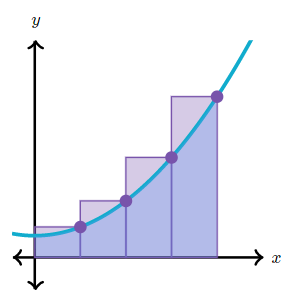
\includegraphics[width=0.25\linewidth]{images/Riemanns_sums.png}
    \label{fig:riemann-sum}
    \caption{Riemann sum}
\end{figure}

Considering the height of the rectangles, there is not much difference between choosing the left and right values, but the right value is usually chosen because it's simpler for calculation. Hence for the $k$-th subinterval $\sqbrac{\dfrac{k-1}{n}, \dfrac{k}{n}}$ where $k=1,\dots,n$, the height of rectangle is $f\brac{\dfrac{k}{n}}$. Thus the area of the $k$-th rectangle is given by
\[ \frac{1}{n} f\left(\frac{k}{n}\right).\]

Therefore, the integral is obtained by summing up the area of $n$ rectangles; that is,
\begin{equation} 
\int_{0}^{1} f(x) \dd{x} = \lim_{n \to \infty} \sum_{k=1}^{n} \frac{1}{n} f\brac{\frac{k}{n}}.
\end{equation}

\begin{exercise}
Find the values of the following expressions:
\begin{enumerate}[label=(\alph*)]
\item $\displaystyle\lim_{n\to\infty}\brac{\frac{1}{n+1}+\frac{1}{n+2}+\cdots+\frac{1}{2n}}$
\item $\displaystyle\lim_{n\to\infty}\frac{1}{n}\brac{e^\frac{1}{n}+e^\frac{2}{n}+\cdots+e^1}$
\item $\displaystyle\lim_{n\to\infty}\frac{\sqrt{n+1}+\sqrt{n+2}+\cdots+\sqrt{2n}}{n\sqrt{n}}$
\item $\displaystyle\lim_{n\to\infty}\brac{\frac{1}{\sqrt{n(n+1)}}+\frac{1}{\sqrt{n(n+2}}+\cdots+\frac{1}{\sqrt{n(4n)}}}$
\item $\displaystyle\lim_{n\to\infty}\frac{1}{n}\brac{\frac{1}{\sqrt{n^2}}+\frac{1}{\sqrt{n^2+1}}+\cdots+\frac{1}{\sqrt{2n^2}}}$
\end{enumerate}
\end{exercise}

\begin{solution} \ 
\begin{enumerate}[label=(\alph*)]
\item \begin{align*}
&\lim_{n\to\infty}\brac{\frac{1}{n+1}+\frac{1}{n+2}+\cdots+\frac{1}{2n}} \\
&= \lim_{n\to\infty}\frac{1}{n}\brac{\frac{1}{1+\frac{1}{n}}+\frac{1}{1+\frac{2}{n}}+\cdots+\frac{1}{1+\frac{n}{n}}} \\
&= \int_0^1\frac{1}{1+x}\dd{x}=\sqbrac{\ln(1+x)}_0^1=\boxed{\ln2}
\end{align*}
Note that in this case $f(x)=\dfrac{1}{1+x}$.

\item \begin{align*}
&\lim_{n\to\infty}\frac{1}{n}\brac{e^\frac{1}{n}+e^\frac{2}{n}+\cdots+e^1} \\
&= \int_0^1e^x\dd{x}=\sqbrac{e^x}_0^1=\boxed{e-1}
\end{align*}
Note that in this case $f(x)=e^x$.

\item \begin{align*}
&\lim_{n\to\infty}\frac{\sqrt{n+1}+\sqrt{n+2}+\cdots+\sqrt{2n}}{n\sqrt{n}} \\
&= \lim_{n\to\infty}\frac{1}{n}\brac{\sqrt{1+\frac{1}{n}}+\sqrt{1+\frac{2}{n}}+\cdots+\sqrt{1+\frac{n}{n}}} \\
&= \int_0^1\sqrt{1+x}\dd{x}=\sqbrac{\frac{2}{3}(1+x)^\frac{3}{2}}_0^1=\boxed{\frac{2}{3}(2\sqrt{2}-1)}
\end{align*}
Note that in this case $f(x)=\sqrt{1+x}$.

\item \begin{align*}
&\lim_{n\to\infty}\brac{\frac{1}{\sqrt{n(n+1)}}+\frac{1}{\sqrt{n(n+2}}+\cdots+\frac{1}{\sqrt{n(4n)}}} \\
&= \lim_{n\to\infty}\sum_{k=1}^{3n}\frac{1}{n}\brac{\frac{1}{\sqrt{1+\frac{k}{n}}}} \\
&= \int_0^3\frac{1}{\sqrt{1+x}}\dd{x}=\sqbrac{2\sqrt{1+x}}_0^3=\boxed{2}
\end{align*}
Note that the sum itself is the sum of $3n$ rectangles, with their heights determined by $f(x)$ from $x=0$ to $x=3$.

\item \begin{align*}
&\lim_{n\to\infty}\frac{1}{n}\brac{\frac{1}{\sqrt{n^2}}+\frac{1}{\sqrt{n^2+1}}+\cdots+\frac{1}{\sqrt{2n^2}}} \\
&= \lim_{n\to\infty}\frac{1}{n^2}\brac{\frac{1}{\sqrt{1+\frac{1}{n^2}}}+\frac{1}{\sqrt{1+\frac{2}{n^2}}}+\cdots+\frac{1}{\sqrt{1+\frac{n^2}{n^2}}}} \\
&= \int_0^1\frac{1}{\sqrt{1+x}}\dd{x}=\sqbrac{2\sqrt{1+x}}_0^1=\boxed{2\brac{\sqrt{2}-1}}
\end{align*}
Note that the interval $[0,1]$ is divided into $n^2$ subintervals.
\end{enumerate}
\end{solution}

\begin{exercise} \
\begin{enumerate}[label=(\alph*)]
\item Prove that for any positive integer $n\ge2$,
\[ 2\sqrt{n}-2<1+\frac{1}{\sqrt{2}}+\frac{1}{\sqrt{3}}+\cdots+\frac{1}{\sqrt{n}}<2\sqrt{n}-1. \]
\item Compare the sizes between $\displaystyle1+\frac{1}{\sqrt{2}}+\frac{1}{\sqrt{3}}+\cdots+\frac{1}{\sqrt{n}}$ and $2\sqrt{n}-\dfrac{3}{2}$.
\item Find the integer part of $\displaystyle1+\frac{1}{\sqrt{2}}+\frac{1}{\sqrt{3}}+\cdots+\frac{1}{\sqrt{2023}}$.
\end{enumerate}
\end{exercise}

\begin{solution} \
\begin{enumerate}[label=(\alph*)]
\item The sum $\displaystyle1+\frac{1}{\sqrt{2}}+\frac{1}{\sqrt{3}}+\cdots+\frac{1}{\sqrt{n}}$ is relevant area under the graph $y=\dfrac{1}{x}$, in the interval $[1,n]$. By integration, this area is $2\sqrt{n}-2$.

On the other hand, consider the area to be approximated by rectangles under the graph, then this approximation is $\displaystyle\frac{1}{\sqrt{2}}+\frac{1}{\sqrt{3}}+\cdots+\frac{1}{\sqrt{n}}$. Because all these rectangles are under the graph, we have
\[ \frac{1}{\sqrt{2}}+\frac{1}{\sqrt{3}}+\cdots+\frac{1}{\sqrt{n}}<2\sqrt{n}-2 \]
or
\[ 1+\frac{1}{\sqrt{2}}+\frac{1}{\sqrt{3}}+\cdots+\frac{1}{\sqrt{n}}<2\sqrt{n}-1. \]

Consider these rectangles to cover the area under the graph. The same area can be covered if we consider the slightly higher rectangles which use the $f$-value of each of the left endpoints. So we have $\displaystyle1+\frac{1}{\sqrt{2}}+\frac{1}{\sqrt{3}}+\cdots+\frac{1}{\sqrt{n-1}}>2\sqrt{n}-2$.

\item Consider the sum of trapeziums instead of just rectangles.

For each interval $[k,k+1]$, we use $f(k)$ and $f(k+1)$ for the two heights of the trapezium. Thus the area of one such trapezium is $\displaystyle\frac{1}{2}\brac{\frac{1}{\sqrt{k}}+\frac{1}{\sqrt{k+1}}}$. Hence the total area over the interval $[1,n]$ is
\[ \frac{1}{2}\cdot1+\brac{\frac{1}{\sqrt{2}}+\frac{1}{\sqrt{3}}+\cdots+\frac{1}{\sqrt{n-1}}}+\frac{1}{2}\cdot\frac{1}{\sqrt{n}}. \]
Since the graph $y=\dfrac{1}{\sqrt{x}}$ is convex, the trapeziums do in fact cover the area under its graph. Thus
\[ \frac{1}{2}\cdot1+\brac{\frac{1}{\sqrt{2}}+\frac{1}{\sqrt{3}}+\cdots+\frac{1}{\sqrt{n-1}}}+\frac{1}{2}\cdot\frac{1}{\sqrt{n}}>2\sqrt{n}-2 \]
or
\[ 1+\frac{1}{\sqrt{2}}+\cdots+\frac{1}{\sqrt{n-1}}+\frac{1}{2}\cdot\frac{1}{\sqrt{n}}>2\sqrt{n}-\frac{3}{2}. \]

\item From (b) we have
\[ 2\sqrt{n}-\frac{3}{2}<1+\cdots+\frac{1}{\sqrt{n}}<2\sqrt{n}-1. \]
Substituting $n=2025$ gives
\begin{align*}
1+\cdots+\frac{1}{\sqrt{2023}} &< 1+\cdots+\frac{1}{\sqrt{2025}} < 2(45)-1=89 \\
1+\cdots+\frac{1}{\sqrt{2023}} &= 1+\cdots+\frac{1}{\sqrt{2025}}-\frac{1}{\sqrt{2024}}-\frac{1}{\sqrt{2025}} \\
&> 2(45)-\frac{3}{2}-\frac{1}{\sqrt{2024}}-\frac{1}{\sqrt{2025}}
\end{align*}
The only thing left to do is to show that $\displaystyle\frac{1}{\sqrt{2024}}+\frac{1}{\sqrt{2025}}<\frac{1}{2}$, which is obviously true.

Hence $1+\cdots+\dfrac{1}{\sqrt{2023}}>2(45)-2=88$ so the integer part is $88$.
\end{enumerate}
\end{solution}
\pagebreak

\section{Double Integrals}
\begin{exercise}
Find the value of the sum
\[ \lim_{n\to\infty}\sum_{k,l=1}\frac{1}{n^2+kl}. \]
\end{exercise}

\begin{solution}
Consider the double integral
\[ \iint_{[0,1]\times[0,1]}f(x,y)\dd{x}\dd{y}. \]
We approximate using cuboids under the graph; split this region up by slicing horizontally and vertically into $n$ slices each. Each cuboid has side length $\frac{1}{n}$, $n^2$ cuboids in total.

Hence
\begin{align*}
&\iint_{[0,1]\times[0,1]}f(x,y)\dd{x}\dd{y} \\
&= \lim_{n\to\infty}\frac{1}{n^2}\sum_{k,l=1}^n\frac{1}{1+\frac{k}{n}\frac{l}{n}} \\
&= \iint_{[0,1]\times[0,1]}\frac{1}{1+xy}\dd{x}\dd{y} \\
&= \iint_{[0,1]\times[0,1]}\brac{1-xy+x^2y^2-x^3y^3+\cdots}\dd{x}\dd{y}
\end{align*}
Note that
\[ \iint_{[0,1]\times[0,1]}x^ky^k\dd{x}\dd{y}=\int_{[0,1]}x^k\dd{x}\int_{[0,1]}y^k\dd{y}=\frac{1}{(k+1)^2}. \]
Hence
\begin{align*}
&\iint_{[0,1]\times[0,1]}\brac{1-xy+x^2y^2-x^3y^3+\cdots}\dd{x}\dd{y} \\
&= 1-\frac{1}{2^2}+\frac{1}{3^2}-\frac{1}{4^2}+\cdots \\
&= \brac{1+\frac{1}{2^2}+\frac{1}{3^2}+\frac{1}{4^2}+\cdots}-2\brac{\frac{1}{2^2}+\frac{1}{4^2}+\cdots} \\
&= \frac{\pi^2}{6}-2\cdot\frac{1}{2^2}\cdot\frac{\pi^2}{6}=\boxed{\frac{\pi^2}{12}}
\end{align*}
where we have applied the solution for Basel's problem.
\end{solution}

Double integrals are usually calculated by integrating the terms one by one.

\begin{exercise}
Find the value of the following integral:
\[ \iint_{[-2,2]\times[-1,1]}x^2|y|^3\dd{x}\dd{y} \]
\end{exercise}

\begin{solution}
\begin{align*}
&\iint_{[-2,2]\times[-1,1]}x^2|y|^3\dd{x}\dd{y} \\
&= \int_{[-2,2]}\brac{\int_{[-1,1]}x^2|y|^3\dd{y}}\dd{x} \\
&= \int_{[-2,2]}\dd{x}\int_{[-1,1]}x^2|y|^3\dd{y} \\
&= 4\int_0^2\dd{x}\int_0^1x^2y^3\dd{y} \quad x^2|y|^3 \text{ is even wrt to both } x \text{ and } y \\
&= 4\int_0^2\sqbrac{\frac{x^2y^4}{4}}_0^1\dd{x} \\
&= \int_0^2x^2\dd{x}=\boxed{\frac{8}{3}}
\end{align*}
\end{solution}

One other simplication method: $x^2|y|^3$ is separable because it is an expression in the form $f(x)g(y)$, and the region of integration is a product set $A\times B$, then
\[ \iint_{A\times B}f(x)g(y)\dd{x}\dd{y}=\int_Af(x)\dd{x}\cdot\int_Bg(y)\dd{y} \]
\begin{proof}
\begin{align*}
&\iint_{A\times B}f(x)g(y)\dd{x}\dd{y} \\
&= \int_A\brac{\int_Bf(x)g(y)\dd{y}}\dd{x} \\
&= \int_A\brac{f(x)\int_Bg(y)\dd{y}}\dd{x} \\
&= \int_Akf(x)\dd{x} \text{ where } k=\int_Bg(y)\dd{y} \text{ is constant wrt } x \\
&= k\int_Af(x)\dd{x} \\
&= \int_Af(x)\dd{x}\cdot\int_Bg(y)\dd{y}
\end{align*}
\end{proof}

\begin{exercise}
Find the values of the following integrals:
\begin{enumerate}[label=(\alph*)]
\item $\displaystyle\int_0^{\sqrt{3}}\dd{x}\int_0^1\frac{8x}{(x^2+y^2+1)^2}\dd{y}$
\item $\displaystyle\iint_D(x+y)\dd{x}\dd{y}$, where $D$ is the region enclosed by $y=e^x$, $y=1$, $x=0$ and $x=1$.
\item $\displaystyle\iint_Dx^2y^2\dd{x}\dd{y}$, where $D$ is the region enclosed by $x^2+y^2=1$.
\end{enumerate}
\end{exercise}

\begin{exercise}
Find the volume of the region enclosed by the surfaces $z=x^2+y^2$ and $z=2x-y+2$.
\end{exercise}

\begin{exercise}
Two numbers $a$ and $b$ are chosen randomly from the interval $[0,2]$. Find the expected value of their product.
\end{exercise}

\begin{exercise}
Two points $P$ and $Q$ are chosen randomly on the line segment $AB$. Find the expected value of the volume of a cuboid of side lengths $AP$, $PQ$ and $QB$.
\end{exercise}
\pagebreak

\section*{Exercises}
\begin{prbm}[\acrshort{smo} (Open) 2020 Q10]
Find the value of 
\[ S = \lim_{n \to \infty} \sum_{k=1}^{n} \frac{1}{\sqrt{n(n+k)}} \]
\end{prbm}
    
\begin{solution}
\[ S = \lim_{n \to \infty} \sum_{k=1}^{n} \frac{1}{n} \sqrt{\frac{1}{1+\frac{k}{n}}} = \int_{0}^{1} \frac{1}{\sqrt{1+x}} \dd{x} = \boxed{2\sqrt{2}-2} \]
\end{solution}

\begin{prbm}[\acrshort{smo} (Open) 2018 Q12]
Given that
\[ S=\lim_{n\to\infty}\sum_{k=1}^n\frac{1}{n+k} \]
Find the value of $S$.
\end{prbm}

\begin{solution}
\[ S = \lim_{n\to\infty}\frac{1}{n}\sum_{k=1}^n\frac{1}{1+\frac{k}{n}} = \int_0^1\frac{1}{1+x}\dd{x} = \boxed{\ln2} \]
\end{solution}

\begin{prbm}[\acrshort{smo} (Open) 2018 Q10]
Find the smallest integer $r$ such that
\[1+\frac{1}{\sqrt{2}}+\frac{1}{\sqrt{3}}+\frac{1}{\sqrt{4}}+\cdots+\frac{1}{\sqrt{2018}}\le r\sqrt{2018}.\]
\end{prbm}

\begin{solution}
Consider Riemann sum of $y=\frac{1}{\sqrt{x}}$. Then
\begin{align*}
&1+\frac{1}{\sqrt{2}}+\frac{1}{\sqrt{3}}+\frac{1}{\sqrt{4}}+\cdots+\frac{1}{\sqrt{2018}}\\
&<\int_{0}^{2018}\frac{1}{\sqrt{x}}\dd{x}\\
&=\sqbrac{\frac{x^\frac{1}{2}}{\frac{1}{2}}}_{0}^{2018}\\
&=2\sqrt{2018}.
\end{align*}
\end{solution}

\chapter{Strategy Games}
\section*{Exercises}
\begin{prbm}[Princess Problem]
On the top floor of a castle lives a princess. The floor has $17$ bedrooms arranged in a row. Each bedroom has doors connecting to the adjoining bedrooms as well as to the outside corridor. The princess sleeps in a different bedroom each night by opening the door to an adjoining bedroom and spending the night and the next day in that room.

One day a prince arrives at the castle and is desirous of marrying the princess. The guardian angel at the castle tells him of the princess' sleeping patterns and informs him that each morning he may knock on one of the outside doors. If the princess happens to be behind that door, she will open it and consent to marry him. The prince also has a return ticket to his kingdom in $30$ days, so he can make at most $30$ attempts. Can the prince win the hand of the princess, and if so, what is his strategy?
\end{prbm}

\begin{solution}
The main idea is that the princess switches parity every day.

The strategy is the Prince should knock on the second door from one of the ends of the corridor (call it door \#2), and knock on the next adjacent door each successive day until he reaches the second door from the opposite end of the corridor (door \#16). The day after that, he should begin the same process in reverse order (meaning he will knock on the 16th door two days in a row). By the time he reaches his starting point (door \#2 on the 30th day), he will have found the princess.

Number the doors 1 thru 17.
If the princess occupies an even numbered room on the day the prince first knocks on a door (\#2), then she will either occupy the same room he knocks on or she will be an even number of rooms away. Since both move to an adjacent room each day, this will hold true so she will never be in a room adjacent to the one he knocks on, and thus never be in a position to move past him the next day. She will have nowhere else to go by the time he reaches the 16th door, and will have by then been located. If she, on the other hand, was in an odd numbered room when he began, then she will be in an even numbered room when the prince starts the process again on day 16 (when he knocks on door \#16 the second time).

To visualise this, the pink squares are rooms where the princess could be on the given day, the blue squares are where the prince knocks that day, and the black squares are rooms in which she logically cannot be. On day 30 all rooms but room 2 have been eliminated, meaning that if the prince has not found the princess already, he will find her there on day 30.

\begin{figure}[H]
    \centering
    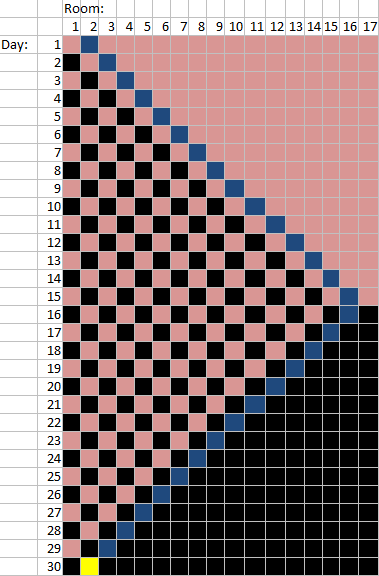
\includegraphics[width=0.5\linewidth]{images/princess-problem.png}
\end{figure}
\end{solution}

% https://cemc.uwaterloo.ca/events/mathcircles/2013-14/Fall/Junior78_Nov19.pdf
% https://www.math.cmu.edu/~mlavrov/arml/12-13/games-02-24-13.pdf
% https://math.mit.edu/research/highschool/primes/materials/2015/Ji-Park-Song.pdf
% https://mathcircle.berkeley.edu/sites/default/files/archivedocs/2015/lecture/BMC_Int2-Sep1-2015-combinatorialgames.pdf
\end{document}